\documentclass{classes/sysuthesis}

\newcommand{\xvec}{\mathbf{x}}
\newcommand{\yvec}{\mathbf{y}}
\newcommand{\Xinput}{\mathbf{X}_{\mathrm{in}}}
\newcommand{\xcommon}{\mathbf{x}_{\mathrm{common}}}
\newcommand{\xproto}{\mathbf{x}_{\mathrm{proto}}}

\newcommand{\xtraffic}{\mathbf{x}_{\mathrm{traffic}}}

\newcommand{\tildey}{\tilde{\mathbf{y}}}
\usepackage{multirow}
\usepackage{tikz}
%%
% 论文相关信息
% 盲审版已匿名化，正式版请恢复作者与导师信息。


% \ctitle{面向高负载与动态流量的5G物联网随机接入机制设计与优化}
\ctitle{物联网海量异构终端随机接入机制优化与智能适配技术研究}
% \etitle{Design and Optimization of 5G Random Access Mechanisms \\ \qquad \qquad \quad \,
	% for High-load and Dynamic Scenarios}
\etitle{Research on Random Access Mechanism Optimization and Intelligent 
\\ \qquad \qquad \quad \,
Adaptation for Massive Heterogeneous Devices in IoT  }

\cauthor{朱威龙}    % 作者中文名
\eauthor{Weilong Zhu}	%作者英文名
\degree{硕士}		%硕士or博士
\studentid{23216076}	%学号
\cschool{电子与通信工程学院}	%学院

\cmajor{信息与通信工程}	%专业名称
\emajor{Information and Communication Engineering}
% 英文专业名称

% 指导教师
\cmentor{詹文 \quad 副教授}
\ementor{Wen Zhan}



% \cauthor{XXX}    % 作者中文名
% \eauthor{XXX}	%作者英文名
% \degree{硕士}		%硕士or博士
% \studentid{XXX}	%学号
% \cschool{XXX学院}	%学院

% \cmajor{信息与通信工程}	%专业名称
% \emajor{Information and Communication Engineering}
% 	%英文专业名称

% % 指导教师
% \cmentor{XXX}
% \ementor{XXX}

     % 论文相关信息
%%
% 摘要信息
% 摘要内容应概括地反映出本论文的主要内容，主要说明本论文的研究目的、内容、方法、成果和结论。要突出本论文的创造性成果或新见解，不要与引言相 混淆。语言力求精练、准确，以 300—500 字为宜。
% 关键词是供检索用的主题词条，应采用能覆盖论文主要内容的通用技术词条(参照相应的技术术语 标准)。按词条的外延层次排列（外延大的排在前面）。


\cabstract{
随着B5G/6G网络向海量终端连接与多样化业务需求持续演进，复杂物联网场景下随机接入过程中的性能瓶颈日益凸显。传统Aloha与CSMA/LBT等接入机制普遍存在按包重复竞争开销较大、信道利用率受限以及对动态业务变化适应能力不足等问题，严重制约系统在高负载与多业务异构环境中的整体性能表现。围绕复杂物联网场景下高效、低开销且可自适应的随机接入核心需求，本文从接入机制优化与系统级决策两个维度开展系统性研究，为B5G/6G网络随机接入系统的性能提升与工程实现提供理论支撑与技术路径。

面向授权频谱短报文接入场景，针对传统Aloha机制重复竞争开销偏高、适配性不足的问题，提出连续传输增强Aloha机制。该机制在保持原有分布式接入结构不变的前提下，通过扩展单次竞争成功后的连续发送能力，有效降低单位数据传输的平均竞争开销，兼顾机制兼容性与性能提升需求。基于休假排队理论构建系统性能分析模型，对吞吐量、信令开销等关键指标进行量化刻画，并结合离散事件仿真验证机制的有效性与可行性。研究结果表明，所提机制可将系统最大吞吐量提升至0.5，突破传统机制性能上限，同时在5G小数据传输场景中显著降低信令开销，具备良好的工程兼容性与实际部署价值。

面向非授权频谱LBT接入场景，针对传统CSMA/LBT机制因频繁侦听、退避导致的系统开销过大、性能受限问题，提出连续传输增强CSMA机制。该机制在完整保留载波侦听与退避核心流程的基础上，引入连续传输策略，有效降低重复竞争带来的资源消耗与效率损失。针对信道侦听与传输时长异构的核心问题，构建基于吸收马尔可夫链的精细化分析模型，对系统吞吐量与接入公平性进行联合刻画与量化分析。理论分析与仿真验证结果表明，该机制在无需额外复杂控制逻辑的前提下，可实现约28.8\%的吞吐量提升，且在效率提升的同时稳定保持良好的系统公平性，适配非授权频谱复杂接入场景需求。

针对动态业务环境中单一接入机制难以持续适配场景变化、无法兼顾多维度性能需求的问题，构建统一的接入性能评估与自适应决策框架。通过离散事件仿真技术，生成覆盖多协议、多参数配置的大规模性能数据集，基于多任务学习模型实现吞吐量、时延、公平性及信令开销等多维性能指标的快速精准预测。在此基础上，设计面向多目标优化的效用函数，实现接入协议选择与参数配置的协同优化，提出自适应决策方法。实验结果表明，该方法在保证较低计算开销的前提下，能够实现动态场景下的快速决策与稳定性能增益，显著提升系统对动态业务环境的适配能力，具备较强的实际部署潜力。

综上，本文从机制设计与系统决策两个层面出发，构建了一套面向复杂物联网场景的低开销、高效率且具备自适应能力的随机接入解决方案，系统提升了B5G/6G 下随机接入的系统综合性能，为随机接入增强机制的工程实现与系统优化提供了重要的理论参考与技术支撑。
}
% 中文关键词(每个关键词之间用;分开,最后一个关键词不打标点符号。)
\ckeywords{5G；随机接入；Aloha；CSMA/LBT；连续传输；休假排队；多任务学习；自适应决策}

\eabstract{
With the continuous evolution of B5G/6G networks towards massive terminal connections and diverse service requirements, the performance bottlenecks in the random access process of complex Internet of Things scenarios have become increasingly prominent. Traditional access mechanisms such as Aloha and CSMA/LBT generally have problems including high overhead caused by packet-by-packet repeated contention, limited channel utilization, and insufficient adaptability to dynamic service changes, which severely restrict the overall performance of the system in high-load and multi-service heterogeneous environments. Centering on the core demand for efficient, low-overhead and adaptive random access in complex Internet of Things scenarios, this paper conducts systematic research from two dimensions: access mechanism optimization and system-level decision-making, providing theoretical support and technical paths for the performance improvement and engineering implementation of random access systems in B5G/6G networks.

For the short packet access scenario in authorized spectrum, aiming at the problems of high repeated contention overhead and insufficient adaptability of traditional Aloha mechanisms, a successive transmission enhanced Aloha mechanism is proposed. On the premise of maintaining the original distributed access structure unchanged, the mechanism effectively reduces the average contention cost of unit data transmission by extending the continuous transmission capability after a single successful contention, balancing mechanism compatibility and performance improvement requirements. A system performance analysis model is constructed based on vacation queuing theory to quantitatively characterize key indicators such as throughput and signaling overhead, and the effectiveness and feasibility of the mechanism are verified through discrete event simulation. The research results show that the proposed mechanism can increase the maximum system throughput to 0.5, break the performance upper limit of traditional mechanisms, and significantly reduce signaling overhead in 5G small data transmission scenarios, with good engineering compatibility and practical deployment value.

For the LBT access scenario in unlicensed spectrum, aiming at the problems of excessive system overhead and limited performance of traditional CSMA/LBT mechanisms caused by frequent listening and backoff, a successive transmission enhanced CSMA mechanism is proposed. On the basis of fully retaining the core processes of carrier sensing and backoff, the mechanism introduces a successive transmission strategy to effectively reduce resource consumption and efficiency loss caused by repeated contention. Aiming at the core problem of heterogeneous channel listening and transmission durations, a refined analysis model based on absorbing Markov chain is constructed to jointly characterize and quantitatively analyze system throughput and access fairness. Theoretical analysis and simulation verification results show that without additional complex control logic, the proposed mechanism can achieve a throughput improvement of about 28.8\%, and stably maintain good system fairness while improving efficiency, adapting to the needs of complex access scenarios in unlicensed spectrum.

Aiming at the problem that a single access mechanism is difficult to continuously adapt to scenario changes and cannot balance multi-dimensional performance requirements in dynamic business environments, a unified access performance evaluation and adaptive decision-making framework is constructed. Large-scale performance datasets covering multi-protocol and multi-parameter configurations are generated through discrete event simulation technology, and a multi-task learning model is used to achieve fast and accurate prediction of multi-dimensional performance indicators including throughput, delay, fairness and signaling overhead. On this basis, a utility function oriented to multi-objective optimization is designed to realize the coordinated optimization of access protocol selection and parameter configuration, and an adaptive decision-making method is proposed. Experimental results show that on the premise of ensuring low computational overhead, the method can achieve fast decision-making and stable performance gains in dynamic scenarios, significantly improve the adaptability of the system to dynamic business environments, and has strong practical deployment potential.

In summary, starting from the two levels of mechanism design and system decision-making, this paper constructs a set of low-overhead, high-efficiency and adaptive random access solutions for complex Internet of Things scenarios, systematically improving the comprehensive performance of random access systems in B5G/6G networks, and providing important theoretical reference and technical support for the engineering implementation and system optimization of random access mechanisms.
}
% 英文文关键词（关键词之间用逗号隔开，最后一个关键词不打标点符号。）
\ekeywords{ 5G; Random Access, Aloha, CSMA/LBT, Successive Transmission, Vacation Queuing Theory, Multi-Task Learning, Adaptive Decision-Making} 
     % 摘要内容

\begin{document}
    % 论文前置部分
    \frontmatter
        \pagenumbering{Roman}
        % \maketitle    % 扉页
       % \makedisclaim       % 原创性及学位论文使用授权声明
        \makeabstract       % 中英文摘要
        \maketableofcontents    % 目录        

        \makelistoffiguretable
        % 缩略语
        %列举文章中出现的专业名词缩略语对应的中文全称和英文全称，注意按首字母顺序排序

\chapter{\heiti{缩略语}}
\begin{longtable}{p{2.5cm}p{8cm}p{5cm}}
	\heiti{缩略语}		&\heiti{英文全称}		&\heiti{中文全称}        \\
	3GPP 		& 3rd Generation Partnership Project 		& 第三代合作伙伴计划 \\
    5G      &5th Generation Mobile Networks     &第五代移动网络\\
    5G NR  &5G New Radio  &5G 新无线技术\\
    ACK  &Acknowledge Character  &确认信令\\
    AWGN &Additive White Gaussian Noise &加性白噪声\\
    CSMA &Carrier Sense Multiple Access &载波侦听多址接入\\
    EDT  &Early Data Transmission &早期数据传输\\
    GSM &Global System for Mobile Communications  &全球移动通信系统\\
    HOL  packet &Head-of-line  packet &队列头包\\
    IEEE &Institute of Electrical and Electronics Engineering &美国电气与电子工程师协会\\
    IIoT &Industrial Internet of Things &工业物联网\\
    ITU     &International Telecommunication Union   &国际电信联盟\\

    LTE  &Long term Evolution  &长期演进\\
    LTE-M &Long term Evolution for Machines &机器类长期演进\\

    M2M &Machine-to-Machine Communications & 机器对机器通信\\
    mMTC &massive Machine Type Communications  &海量机器类通信\\
    MTC & Machine Type Communications & 机器类通信\\
    mURLLC  &massive Ultra Reliable and Low Latency Communications  &海量超可靠低时延通信\\

    NAK  &Negative Acknowledgment  &否定信令\\
    NB-IoT &Narrow Band Internet of Things &窄带物联网\\

    QoS &Quality of Service &服务质量\\
    RACH &Random Access Channel  &随机接入信道\\
    SNR   &Signal to Noise Ratio    &信噪比\\
    UMTS &Universal Mobile Telecommunications System &通用移动通信系统\\
    URLLC &Ultra Reliable and Low Latency Communications &超可靠低时延通信\\

										
\end{longtable} 

        % 数学符号
        % 汇总全文中出现的主要数学符号及其含义

\chapter{\heiti{数学符号}}

\begin{longtable}{p{4.0cm}p{11.0cm}}
    \toprule
        \heiti{符号} &\heiti{含义}\\
        \midrule
        \endfirsthead

        \toprule
        \heiti{符号} &\heiti{含义}\\
        \midrule
        \endhead

        \midrule
        \multicolumn{2}{r}{\small（续表）}\\
        \endfoot

        \bottomrule
        \endlastfoot

        % 第二章符号
        $n$ &网络节点总数\\
        $\lambda$，$\hat{\lambda}$  &单节点到达速率/网络平均到达率\\
        $p_{ne}$ &节点缓存非空概率\\
        
        % 第三章符号
        $B,\ V,\ C$ &节点忙期/假期/周期长度（$C=B+V$）\\
        $\lambda_{\mathrm{out}},\ \lambda_{\mathrm{out}}^a,\ \lambda_{\mathrm{out}}^d$ &系统吞吐量；接入吞吐量；数据吞吐量\\
        $\Theta,\ \theta$ &任意空闲时隙内聚合接入请求总数随机变量；接入请求速率（尝试速率，饱和时记为 $\theta_{sa}$）\\
        $q$ &节点在缓存非空时发起接入尝试的概率\\
        $A_B,\ A_V$ &节点在忙期/假期内的新到达包数\\
        $Q_t,\ P_t,\ Q,\ P$ &队列长度随机变量（时变/稳态）\\
        $G_Q(z),\ G_P(z)$ &概率生成函数（PGF）\\
        
        % 第四章符号
        $B_c,\ V_c,\ C_c$ &信道忙期/假期/周期长度（$C_c=B_c+V_c$）\\
        $\overline{B},\ \overline{V}_c,\ \sigma_B^2,\ \sigma_{V_c}^2$ &信道忙期/假期均值及其方差\\
        $p_0,\ p_1,\ p_2$ &无节点发送概率；恰有一个节点发送概率；至少两个节点发送概率\\
        $x,\ y$ &碰撞检测所需时隙数；成功传输时隙数\\
        $\tau_I,\ \tau_F,\ \tau_S$ &空闲侦听/碰撞失败/成功状态持续时间\\
        $\mathbf{P},\ \mathbf{T},\ \mathbf{R}$ &马尔可夫链转移矩阵及其分块\\
        $\mathbf{N}$ &基本矩阵（$\mathbf{N}=(\mathbf{I}-\mathbf{T})^{-1}$）\\
        $\boldsymbol{\mu},\ \mathbf{F}$ &驻留时长向量及其加权和\\
        $\eta$ &有效吞吐时间修正因子\\
        $D$ &平均数据包时延\\
        $J_T$ &公平性指标（Jain 指数）\\
        
        % 第五章符号
        $T$ &仿真或观测时隙总数\\
        $\mathbf{A},\ X(t)$ &到达矩阵（行为节点，列为时隙）；网络聚合到达序列\\
        $\mathcal{T}_i,\ \Delta t_i^{(k)}$ &节点 $i$ 的到达时刻集合；到达间隔序列\\
        $\mathrm{BI}_{\mathrm{net}},\ \mathrm{BI}_{\mathrm{node}}$ &网络突发度指标；节点突发度指标\\
        $\Psi_{\mathrm{net}},\ \Psi_{\mathrm{node}}$ &网络周期性强度；节点周期性强度\\
        $\mathrm{CV},\ \mathrm{ID}$ &变异系数；离散指数（Index of Dispersion）\\
        $\mathbf{x}_{\text{traffic}},\ \mathbf{x}_{\mathrm{common}}$ &业务流量特征向量；通用网络参数向量\\
        $\mathbf{x}_{\mathrm{proto}},\ \mathbf{m}$ &协议专属参数向量；有效性掩码向量\\
        $\mathbf{y},\ \tilde{\mathbf{y}}$ &性能指标向量；归一化后的指标向量\\
        $\hat{y}_k$ &第 $k$ 个任务的预测输出\\
        $S(\cdot)$ &统一仿真映射（从输入到性能指标的映射）\\
        $\mathrm{norm}(\cdot)$ &指标归一化算子\\
        $U(\cdot)$ &综合效用函数\\
        $w_i,\ \omega_k$ &效用加权系数；任务加权系数\\
        $a,\ \mathcal{P}$ &候选协议类型标识；候选协议集合\\
        $a^*,\ \mathbf{x}_{\mathrm{proto}}^*$ &最优协议类型；最优参数配置\\
        $\mathcal{X}_a$ &协议 $a$ 的合法参数空间\\
        $M,\ L,\ T_{\mathrm{frame}}$ &连续传输长度；副本/重传次数；帧长度\\
        $C_{\mathrm{rx}},\ I_{\mathrm{impl}}$ &接收端计算负荷；协议实现复杂度\\
        $C_{\max},\ I_{\max}$ &资源阈值（计算负荷、实现复杂度）\\
        $D_{\text{in}},\ D_{\text{hidden}}$ &神经网络输入维度；隐藏层维度\\
        $\mathbf{h}^{(\ell)},\ \mathbf{W}^{(\ell)}$ &第 $\ell$ 层的隐藏特征；第 $\ell$ 层的权重矩阵\\

        $\mathcal{L}_{\text{total}}$ &多任务总损失函数\\
        $\text{MSE},\ \text{MAE}$ &均方误差；平均绝对误差\\
        $\rho$ &归一化网络负载\\

\end{longtable}


        \newclearpage

    % 论文主体部分
        \mainmatter
        % 引言

        % 正文
        %%
% 引言或背景
% 引言是论文正文的开端,应包括毕业论文选题的背景、目的和意义;对国内外研究现状和相关领域中已有的研究成果的简要评述;介绍本项研究工作研究设想、研究方法或实验设计、理论依据或实验基础;涉及范围和预期结果等。要求言简意赅,注意不要与摘要雷同或成为摘要的注解。
\chapter{绪论}
\label{chapter1: introduction}
%定义，过去的研究和现在的研究，意义，与现有结论的区别

\section{绪论}
\label{sec:background}
% What is the problem
% why is it interesting and important
% Why is it hards, why do naive approaches fails
% why hasn't it been solved before
% what are the key components of my approach and results, also include any specific limitations，do not repeat the abstract
%contribution
%引言是论文正文的开端，应包括毕业论文选题的背景、目的和意义；对国内外研究现状和相关领域中已有的研究成果的简要评述；创新点；介绍本项研究工作研究设想、研究方法或实验设计、理论依据或实验基础；涉及范围和预期结果等。要求言简意赅，注意不要与摘要雷同或成为摘要的注解。

\subsection{选题背景}


第五代移动通信系统（5G）已经大规模商用，在推动我国经济高质量发展、提升产业水平和服务群众生活中发挥了重要作用。然而，随着海量智能终端的普及以及网络化，社会工业生产对移动通信的需求不断增长，全新的应用场景不断涌现，5G 将难以满足未来通信需求。关于超五代 (Beyond 5G, B5G) 通信网络关键技术的研究正当其时。B5G 关键技术的研发需要响应不同业务场景的需求。作为 5G/B5G/6G 的重要业务场景，在当前的5G及即将到来的B5G（Beyond 5G）场景下，物联网（IoT）技术实现了更广泛的应用，成为智能互联设备与环境的核心驱动力。5G网络凭借高带宽、低延迟、超高可靠性和大规模连接能力，显著提升了物联网设备的连接效率，为各行业的数字化转型铺平了道路。海量机器型通信（massive Machine Type communications，mMTC）是指通过在机器上安装各种传感器和控制器等器件，来赋予机器智能的属性，使得机器与机器间能在无人控制的情况下，自主的进行数据交互的技术。mMTC业务场景主要解决大规模设备连接的需求，涵盖众多物联网新兴产业，比如数字低空产业、智慧港口和智慧医疗等，均为《2024 年广东省数字经济工作要点》中所指明的广东省重点发展领域。2023 年，mMTC 也被国际电信联盟无线通信部门（Radio Communication Division of the International Telecommunication Union， ITU-R）纳入 6G 业务愿景。因此，展开针对物联网业务场景的 B5G 关键技术研发对信息技术产业发展具有重要现实意义。

与传统的以人为中心的通信（Human Type Communications, HTC）不同， mMTC 业务场景具有海量接入、零星/短包传输、电量极度受限和上行为主等新流量特征。针对业务流量新特征，NB-IoT、LTE-M 和 LoRaWAN 等新技术或者系统被提出。相比 HTC，针对 mMTC 所设计的不同通信系统虽然网络架构和硬件设计等方面存在显著差异，但共同特征是 MAC 层普遍采纳了免授权随机接入机制(Grant-Free Random Access, GFRA)。在蜂窝网络场景下，GFRA 与传统的授权随机接入（Grant-Based Random Access, GBRA）有本质区别。

\begin{itemize}
	\item GFRA是指设备间通过随机接入协议，分布式共享的时频资源，数据报文直接参与信道竞争。
	\item GBRA是指设备先通过随机接入过程与基站建立空口承载链路，然后基站运用集中式资源调度算法，分配独占的时频资源给设备传输数据。
\end{itemize}

相比GBRA，在GFRA中，基站无需获知设备数据流量特征的先验信息，利用统计复用效应，让不宽裕的时/频/码资源支撑大量潜在设备的接入需求；另一方面，由于基站不需要与每个设备建立空口承载链路，基站运算和空口信令交互开销被大幅降低。因此，GFRA已被纳入蜂窝网络标准体系，GFRA和GBRA将共存于5G/B5G/6G网络已成为业界共识。然而，随物联网业务种类愈发繁杂、流量特征和服务质量要求愈发差异化，从MAC层协议角度，5G现有的GFRA和GBRA协议越来越难以高效支撑各类物联网业务。



\subsection{研究目的及意义}
%4.总结需求并引出选题意义
针对不同物联网业务场景下的随机接入机制协议，业界和学术界围绕GFRA和GBRA展开了系统性的性能分析和对比工作。从数据传输资源的调度模式差异可以看出，采用分布式接入的GFRA适用于零星、小数据报文传输的mMTC业务场景；采用集中式控制的GBRA适用于吞吐量较大或者频繁传输数据的mMTC/HTC业务场景。\cite{bibid}从信令开销的角度，提出了GF RA和GBRA共存5G网络中的接入机制选择策略，阐明了关于数据流量特征或者服务质量要求的判决门限。然而，在有限选项中择优选取，仅能实现相对最优。当物联网流量特征处于接入机制判决门限周边的范围——即流量既非零星/短包传输，也非大吞吐/频繁传输的场景时，GFRA和GBRA均无法为物联网业务提供高效的通信服务。选择GFRA可能因数据流过于密集而导致随机接入信道严重拥堵；而GBRA则可能由于数据流量偏低，造成不必要的接入成本上升，资源浪费，能耗增加。为适应于复杂多变的物联网流量特征，亟需研发创新的MAC层接入机制，以填补现有方案的空白，优化整体网络性能。
现有5G免授权随机接入机制（GFRA）的一个关键缺陷就在于僵化的资源利用模式。以5G NR两步随机接入为例，其沿袭了时隙Aloha协议的思路。设备每个数据报文在每个时隙（或时频资源块）以一定概率传输。每次传输决策仅针对当前的时频资源、至多争用一个时频资源块。在零星小报文mMTC场景下，由于信道负载轻且设备报文少，上述模式有效、可行。如果有多个数据报文需要传输时，受制于资源利用模式和决策机制，设备需要多次决策、多次竞争，导致资源利用率低下，接入信令/能量开销过高。
在本课题的前期工作中发现，破除5G接入机制僵化的资源利用模式的一个简单、直接和有效的方法即是充分利用随机接入信道的短时可用性。大量的仿真统计结果表明，在现有GFRA体制下，由于全网设备传输行为的随机性，单个设备在占用信道一个时隙后，信道实际上会有一定的概率存在连续空闲的情况。充分利用信道的短时可用性能提高随机接入信道的利用率，使得蜂窝系统在不增加时/频/码资源、不变更物理层信号处理体制的前提下，容纳更多的物联网设备和数据，具有重要的理论和工程意义。

具体而言，本课题首先提出一种动态接入时长的免授权接入机制（Dynamic Time-GFRA, DT-GFRA）。在DT-GFRA中，物联网设备采用单次决策、连续传输的机制，即在任一时隙，以一定概率决定传输后，设备将以非独占的形式，在信道上持续传输，直至队列为空、或者因信道衰落、或者因其他节点发起传输而造成干扰中断。该机制预期将至少有如下优势:
\begin{itemize}
	\item 承接传统固定时长的免授权随机接入机制（Fixed Time-GFRA, FT-GFRA）优势，DT-GFRA也不需要设备与基站建立空口承载连接，有效降低信令开销和能耗。
	\item 相比FT-GFRA，DT-GFRA在接入策略上更加弹性和激进，以快速报文续传的模式，利用信道的短时可用性，有效提升网络容量。
	\item DT-GFRA从MAC层协议上创新，无须更改物理层设计，具有广泛的兼容性、实用性和可行性，为B5G网络接入机制设计带来重要理论启示和实现可能。
\end{itemize}

然而如同其他所有类型的随机接入协议，DT-GFRA协议下的网络性能与接入控制参数、资源配置参数等息息相关。为此，本课题将立足3GPP标准协议，围绕物联网业务场景，针对DT-GFRA机制，解决三个问题：如何分析、如何优化及如何实施。具体来说，本课题将重点研究在DT-GFRA机制下，业务流量特征参数和网络参数对MTC设备接入行为与信道占用状况影响机理；运用排队论，构建低复杂度、可优化Markov模型；在复杂物联网业务场景下，进一步引入强化学习算法，提升DT-GFRA的适用广度与能力；基于5G NR两步随机接入协议流程，从信令交互流程的角度，探讨DT-GFRA在蜂窝网络中的实施途径。
本课题旨在设计创新的DT-GFRA机制，突破传统FT-GFRA僵化的资源利用模式、提升网络能效，并构建从理论建模、性能优化到应用实施的完整的理论及技术方案，丰富B5G网络MAC层接入协议体系。


\section{国内外研究现状和相关工作}


作为蜂窝网络标准制定组织3GPP指定的5G三大业务场景之一，海量机器型通信（mMTC）已是学界和工业界研究的焦点。围绕物联网场景的接入机制研究，当前研究工作大致可以分为三类：（1）接入机制设计、（2）网络参数优化和（3）物理层改进。
\subsection{接入机制设计}

早在2010年，3GPP就启动了关于mMTC的接入网（Radio Access Network，RAN）改进项目，发布3GPP TR 37.868文档，阐述了RAN对mMTC业务承载能力的局限性，并围绕接入控制，提出了RAN改进的方向\cite{bibid}。对于4G LTE网络而言，其技术体系面向以人为中心的通信（Human Type Communications, HTC）进行设计，接入机制采用GBRA思想，其随机接入过程基于时隙Aloha协议，即用户节点在每个随机接入信道（Physical Random Access Channel, PRACH）时隙，独立的决定是否发送接入请求\cite{bibid}。由于PRACH资源有限，海量的mMTC接入请求将导致PRACH的严重拥塞和网络瘫痪。同时，mMTC接入后，往往仅传输少量的数据报文。建立空口承载所引发的信令/能耗开销超过数据报文传输量及效益，凸显了GBRA支撑mMTC的局限性\cite{bibid}。针对mMTC业务小数据报文传输的特征，3GPP在保留传统的GBRA的同时，为5G蜂窝网络引入固定时长的免授权随机接入机制（Fixed Time-GFRA, FT-GFRA），也就是四步/两步随机接入过长\cite{bibid}。GFRA制式下，设备在随机接入过程中就已经完成报文传输，不再额外需要搭建无线资源控制层（Radio Resource Control，RRC）资源连接，从而大大降低信令开销\cite{bibid}。目前GFRA被公认为是蜂窝网络支撑mMTC业务的主流范式。

除了以上由3GPP主导改进的接入机制，学者从整个蜂窝系统架构的角度提出更多新颖的策略。例如[10]-[12]提出多层汇聚接入机制，即mMTC设备首先通过非授权频段的Device-to-Device链路将数据报文汇聚至中心节点，然后再由中心节点与基站进行通信，以此大幅降低PRACH信道拥塞，提升单次接入所传输的数据量和能效。[13]-[16]设计了Tree-Splitting接入机制去灵活协调随机接入资源，即为每一个发生报文碰撞的PRACH时频资源块，调度额外的两至三个PRACH时频资源块，通过持续迭代，不断地降低单个PRACH时频资源块上的竞争用户量，直至确保每个用户成功接入。[17]-[19]考虑运用多种空口接入技术支撑mMTC业务，即除了5G蜂窝网络外，系统还可以利用其他的通信技术，例如低功耗广域网络通信技术和低轨卫星通信技术，通过增加空口接入技术冗余度，提升mMTC通信的可靠性。虽然仿真结果显示上述新颖的接入策略能明显提升蜂窝网络接入效率，但网络架构及通信协议需要大幅变更，短时内现实可行性低。

\subsection{网络参数优化}

基于给定的接入机制（包括授权接入或者是免授权接入），通过优化网络参数（包括时频资源、冲突退避和功率等）配置，提升随机接入效率是目前大部分学者所关注的主要研究方向。网络参数优化有两个重要的切入点：流量调度和资源调度。流量调度通过退避机制实现。退避参数主要是MAC层的Backoff窗口和RRC层的Access Class Barring因子。其本质都是让接入失败的UE回退一段随机的时长，再重新发起接入请求，以使海量的、突发的流量在时域上扩散平缓，降低单个时隙的接入请求数量，从而缓解拥塞。资源调度主要包括调度物理随机接入信道（Physical Random Access Channel, PRACH）的时频资源和随机接入前导序列码（Preamble）资源。为合理的调度流量和资源，针对接入性能优化，学者们提出了各种基于接入信道负载的流量调度和资源调度算法，比如根据信道环境，自适应的调整接入请求传输概率[20]、[21]、前导序列资源数目[22]-[24]，随机接入时隙资源数目[23]等。本课题组中立足3GPP MAC层标准协议，针对接入请求，构建了基于Markov状态转移的行为模型，探索了4G/5G网络随机接入信道的极限性能和最佳退避/资源参数的配置方案[25]-[27]。上述参数优化方法依赖于明确的数学模型，然而受限于复杂度，难以扩展至多业务场景或者是动态业务场景。
近年来，运用机器学习算法，特别是强化学习算法，动态优化网络参数，提升随机接入机制性能已成为研究热点。将每个设备视为一个独立的智能体，让其在每个时隙决定是否传输，是目前相关研究的主流切入点。在同构场景中，一些研究者将信道模拟为多信道结构，从频域方向解决相应的动态多信道接入问题。例如，[28]结合Q-Learning 和深度神经网络（Deep Neural Network，DNN）的方法，并提出了一种 DQN 模型。该模型以时间序列的历史观测为输入，通过预测近似的 Q 值, 指导用户如何在多信道环境中灵活切换，以优化频谱的使用。尽管如此，存在的局限性不容忽视。当涉及的信道数量增加时，模型的训练周期随之延长，这会导致实时性能下降，不利于应对快速变化的无线环境。此外，面对大规模的网络用户群体，所提方法依赖于一个集中式控制器来进行信道的分配和冲突管理。这个控制器在每个时间槽中负责选择一个最优的非正交信道子集，并为每个用户分配信道以避免潜在的信号冲突。然而，这种集中式计算策略不仅计算负荷重，而且可能需要大量的信令交互，带来了显著的通信开销，在大型或分布式网络的实际部署中仍需进一步优化以满足效率和可伸缩性的需求。近年，多智能体强化学习（Multi-Agent Reinforcement Learning，MARL）由于其解决高维决策问题以及快速收敛到协作策略的能力，被考虑应用于多址接入机制设计中。例如，[29]中采用 QMIX 算法设计的 QLBT（QMIX-advanced Listen-Before-Talk）多址接入机制，实现比 CSMA/CA 更高的吞吐量和更低的平均延迟，[30]基于多智能体深度确定性策略梯度（Multi-Agent Deep Deterministic Policy Gradient， MADDPG）算法提出了一种联合学习信道访问策略的多址接入机制，在吞吐量方面取得了良好的性能。[31]-[34]则围绕异构随机接入场景展开强化学习算法设计。课题团队在前期工作[35]提出了一种基于多智能体近端策略优化的新型MAC协议，通过在线多智能体强化学习，提升随机接入效率和公平性，同时减少通信开销。


\subsection{物理层改进技术}

通过引入massive MIMO、编码和非正交多址技术等物理层技术，提升系统容量，是目前学者们探索未来B5G/6G mMTC通信场景的一条重要技术路线。以非正交多址技术为案例，学者们分析了基于各类非正交多址接入技术的复杂接收机的性能，例如Gain Division Multiple Access (GDMA)[36], Sparse Code Multiple Access (SCMA)[37], Pattern Division Multiple Access (PDMA)[38]， Resource Spread Multiple Access (RSMA)[39] 和 Irregular Repetition Slotted Aloha [40]等。在[41]中，作者就基于经典的Bianchi模型分析了在非正交多址接入技术体系下，FT-GFRA的吞吐和时延性能，其结果显示非正交多址接入技术，相比传统的正交多址接入技术，可以大幅提升面向报文的随机接入机制。然而，非正交多址接入技术对系统信号处理能力和运算能力提出了较高的要求，不适用于以低功耗、低成本为特点的机器型通信网络，难以短期内在3GPP框架内实现应用落地。

\subsection{国内外文献分析小结}
综上所述，以提升免授权随机接入机制(Grant-Free Random Access, GFRA)性能为目标，现有文献在随机接入机制设计、网络参数优化方法和物理层改进技术等方面已经做了深入探索。然而，对极限接入性能的进一步提升往往伴随网络架构、协议体系和物理层收发信机的大幅改动，短时间内的现实可行性较低。如何在蜂窝系统框架下，通过3GPP协议扩展，设计创新性的接入机制，弥补传统固定时长的免授权随机接入机制（Fixed Time-GFRA, FT-GFRA）的缺陷，实现B5G网络对未来物联网业务的高效的支撑能力，仍是有待解决的问题。



\section{本文研究目标与内容}


\subsection{本文创新点与主要贡献}

本课题提出了一种新型的随机接入机制，即动态时长的免授权接入（DT-GFRA），并且以休假排队论以及多智能体强化学习算法为分析框架，在单/多业务场景条件下，揭示DT-GFRA的各项网络性能。此外，DT-GFRA可以很好兼容于现有的5GNRMAC层，不需要对物理层进行大幅度改动。预期创新点如下：
\begin{itemize}
\item[1.]
提出一种新型随机接入机制，即DT-GFRA。该机制可以很好兼容于现有5G NR的MAC标准，不需要大幅度改动物理层。

\item[2.]
利用休假排队模型构建对于DT-GFRA的分析框架，获得在饱和/不饱和场景下，吞吐/时延等网络指标的显式表达式。以指标表达式为基础，通过调整网络参数实现性能优化，并分析协议性能极限。

\item[3.]
利用多智能体强化学习算法，设计适应于DT-GFRA机制的强化学习框架。

\item[4.] 
能效为目标，给出现有FT-GFRA和GBRA，加上新提出的DT-GFRA三种机制在不同流量场景下的最优接入机制选择方案。

%到6G移动通信网络设计的灵活性和拓展性原则，以及
%在文献\cite{dai2012stabilitydelayofBA}的Aloha网络解析框架基础上创新性地引入了丢包机制。尽管在一定程度上对传输可靠性和能量效率造成了损失，但该机制的引入从建模层面增强了网络的时延性能表现。而重传限制$M$作为一个可调的系统参数，增加了通信系统的设计自由度，进而从性能优化层面增强了灵活性和拓展性。

\end{itemize}

\section{论文结构安排}
\label{sec:arrangement}
本文共分为六章，各章节内容安排如下：

第一章绪论。该章节系统详细地阐述了本文的选题背景意义、国内外研究现状和不足以及本文的创新点和贡献。

第二章系统建模。该章节首先给出通信网络所处的场景和假设。引入了基于吞吐量时延等概念，并给出了一种休假排队模型框架，为后续章节的分析提供基本分析视角。

第三章是基于ALoha的连续传输分析框架。

第四章是基于CSMA的连续传输分析框架。该章节在第二章建模的基础上推导出时延指标关于关键网络参数的闭式解。

第五章是实际通信系统的连续传输机制应用。该章节在前面两章基础上给出实际通信系统的应用。

第六章是本文的最后一章,总结与展望。是对本文内容的整体性总结以及对未来工作的预期。


%\begin{figure}[h]
%\centering 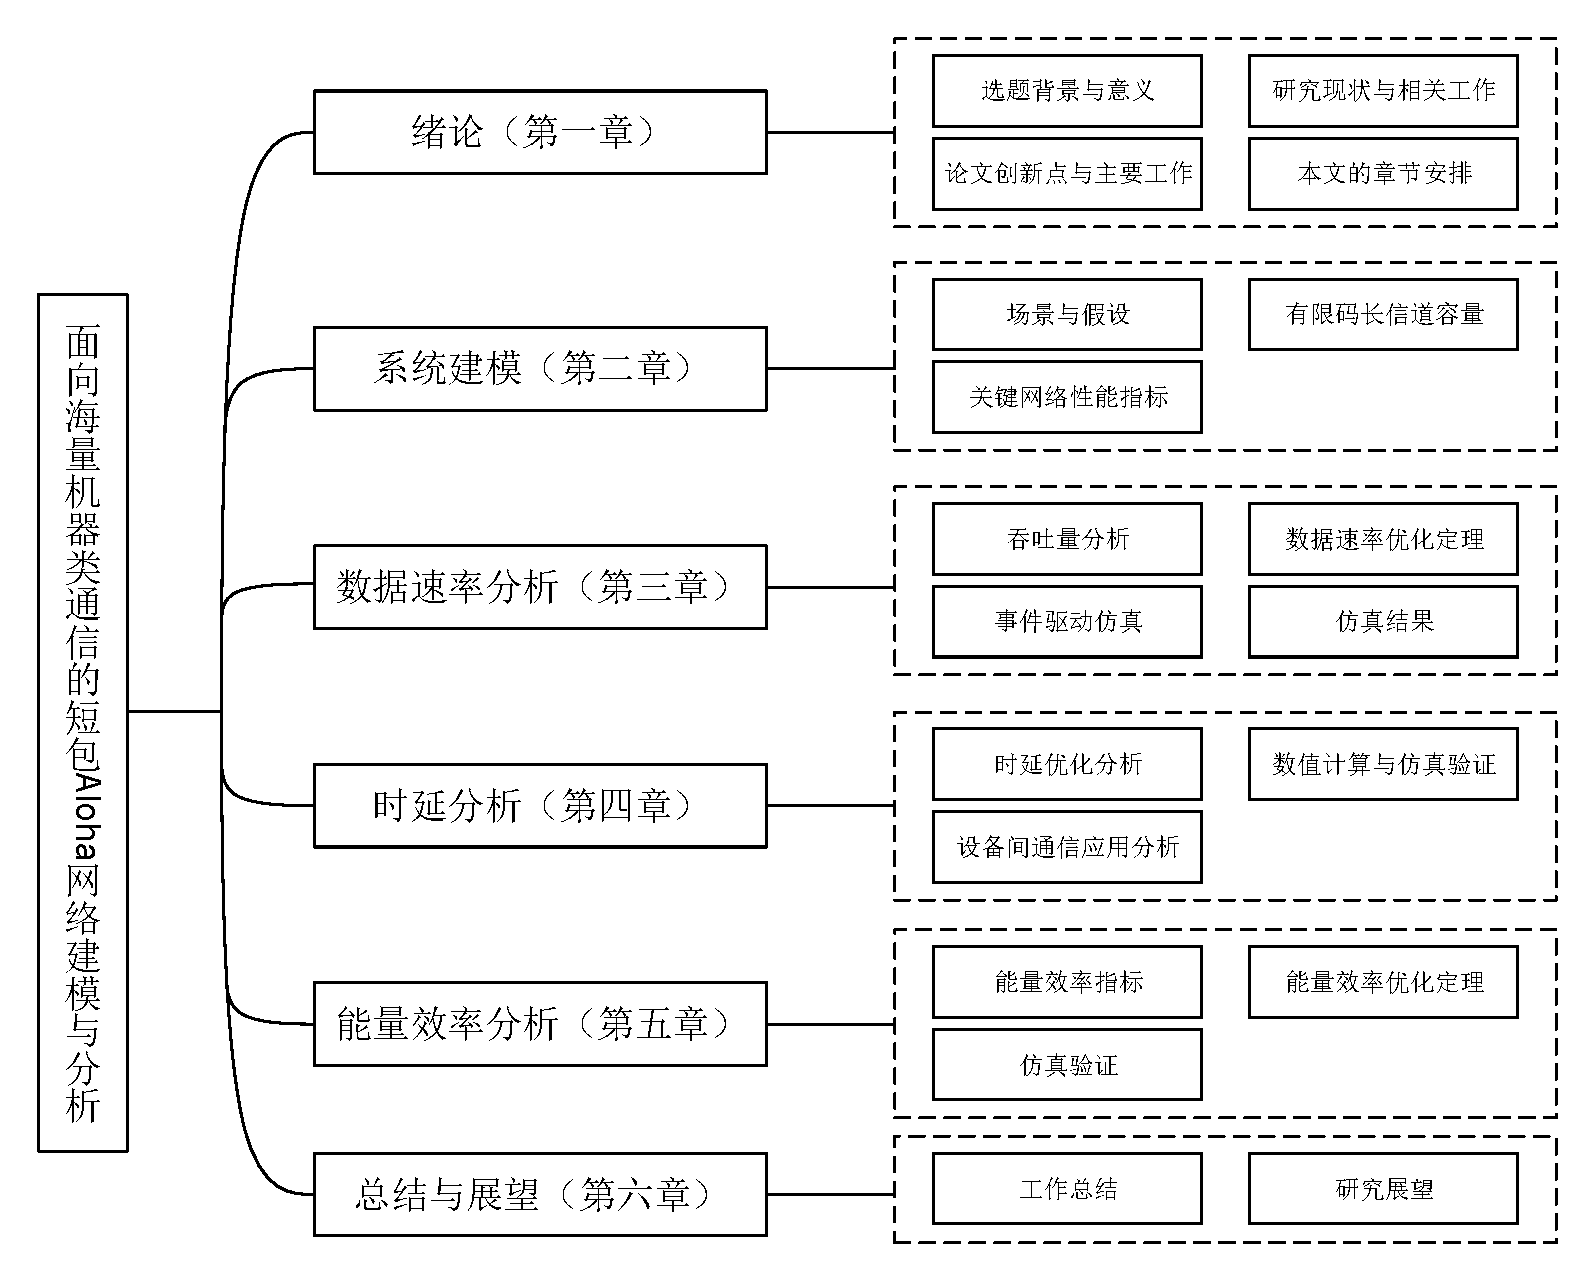
\includegraphics[angle=0,width=155mm,height=125mm]{image/weihua/structure.pdf}
%	\caption{论文章节安排}
%\label{fig:structure}
%\end{figure} 
        \newclearpage
        \chapter{随机接入网络及其建模方法}
\label{chapter2: system model}

本章旨在构建全篇论文的研究基石，对相关的理论背景、核心机制及系统模型进行系统性阐述。章节内容安排如下：首先，回顾现有的主流随机接入标准方案，重点剖析面向 5G 的概率性接入机制与面向非授权频段的载波侦听机制，在总结其技术演进路线的同时揭示现有方案的局限性，从而引出本文的研究动机；其次，深入解析连续传输机制（Successive Transmission）的基本原理，论证其在提升信道利用率方面的内在优势；接着，引入用于后续性能量化分析的核心数学工具——离散时间休假排队理论；最后，为了实现不同协议间性能的公平对比，统一构建了包含网络拓扑、信道特性及业务假设的通用系统场景模型，并定义了关键性能评估指标。

\section{典型随机接入标准方案及其演进}
\label{sec:standard_schemes}

本节从\textbf{机理分析}与\textbf{数学抽象}的视角，对现有随机接入协议的内在结构进行解构。我们不重点讨论应用场景与标准演进，而是聚焦于协议在MAC层的本质运作原理，并并建立与经典随机接入模型之间的对应关系。该抽象框架为后续连续传输机制设计（第~\ref{chapter3: SAST }、\ref{chapter4: CSMAST } 章）
以及 AI 多协议选择（第~\ref{chapter5: ai_selector} 章）提供统一理论基础。

\subsection{基于连接的5G NR随机接入过程}
\label{subsec:cba_mapping}
\begin{figure}[t]
	\centering
	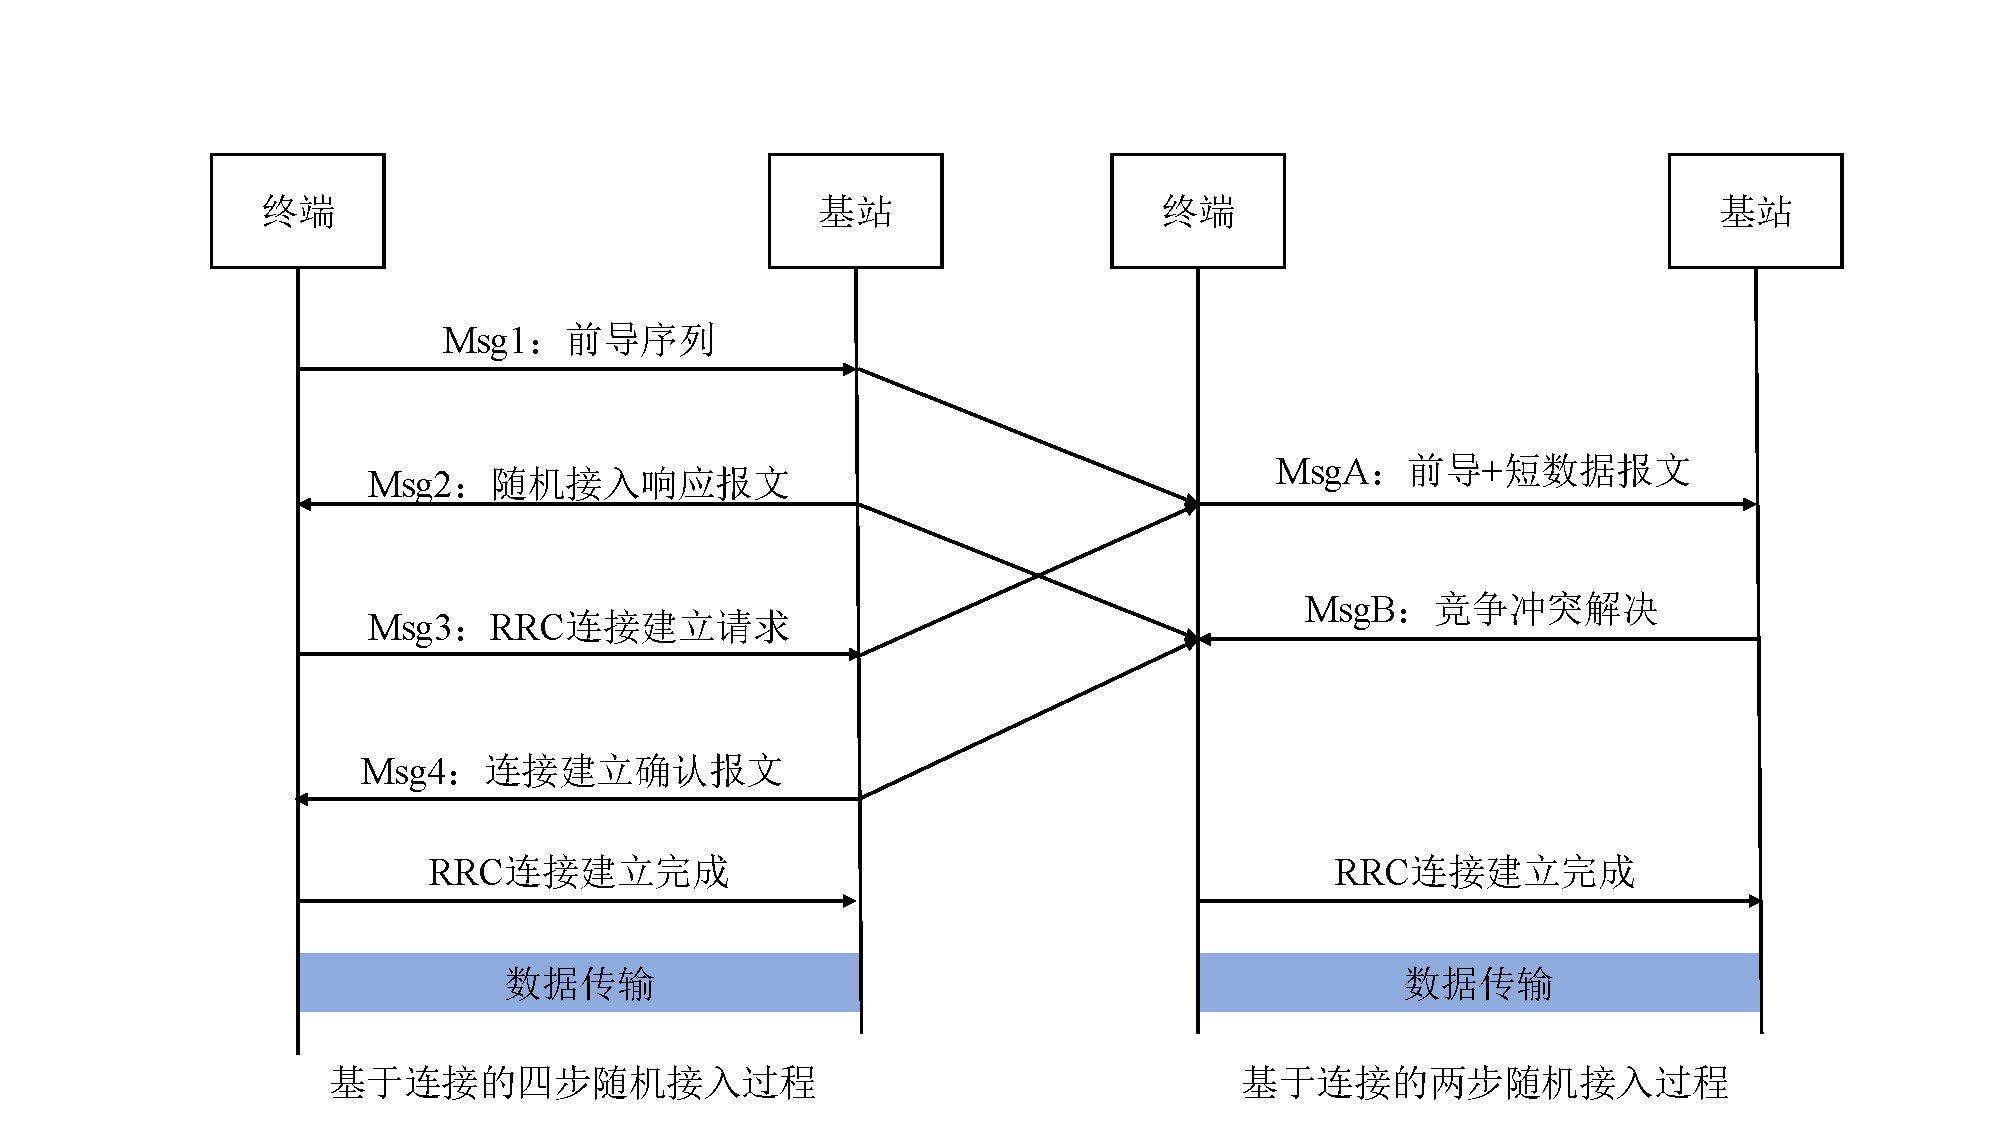
\includegraphics[width=0.95\linewidth]{figure/chap2/5G NR标准随机接入过程.pdf}
	\caption{5G NR 四步/两步标准随机接入流程示意图}
	\label{fig:cba_access}
\end{figure}

5g NR 随机接入过程，从先前的 4G LTE 随机接入过程演变而来。在 5G NR 的基于连接的数据传输模式下，终端在初始随机接入成功后，由基站分配专用无线资源，并在连接期间进行数据传输。现提出的标准方案中存在四步接入和两步接入两种流程，前者在竞争阶段包含更多的握手消息以提高可靠性，而后者则通过合并前导码与数据包来降低接入时延。两种流程图表示如\ref{fig:cba_access}所示。

从接入机理上看，无论四步还是两步，都具有明显的两阶段结构：（1）竞争建立阶段：终端通过随机接入获得资源授权；（2）独占传输阶段：终端在被分配资源上进行连续数据发送。第一阶段与 Slotted Aloha 具有相同的概率竞争特征，而第二阶段则表现为无竞争的资源独占。

因此，可将该结构抽象为一种竞争-预留模型，记为$\text{CBA}(q, M)$,其中：$q$ 为接入阶段的竞争概率；$M$ 为一次竞争成功后可连续占用的传输时隙数。当 $M=1$ 时，该模型退化为标准 Aloha；当 $M>1$ 时，竞争成本可在多个数据包之间分摊，从而提升单位数据的有效吞吐效率。
因此，5G 基于连接的数据传输机制在 MAC 层抽象上可视为 Connection-Based Aloha 的一种实现。

\subsection{面向短报文传输的5G NR随机接入机制}
\label{subsec:sdt_mapping}
\begin{figure}[t]
	\centering
	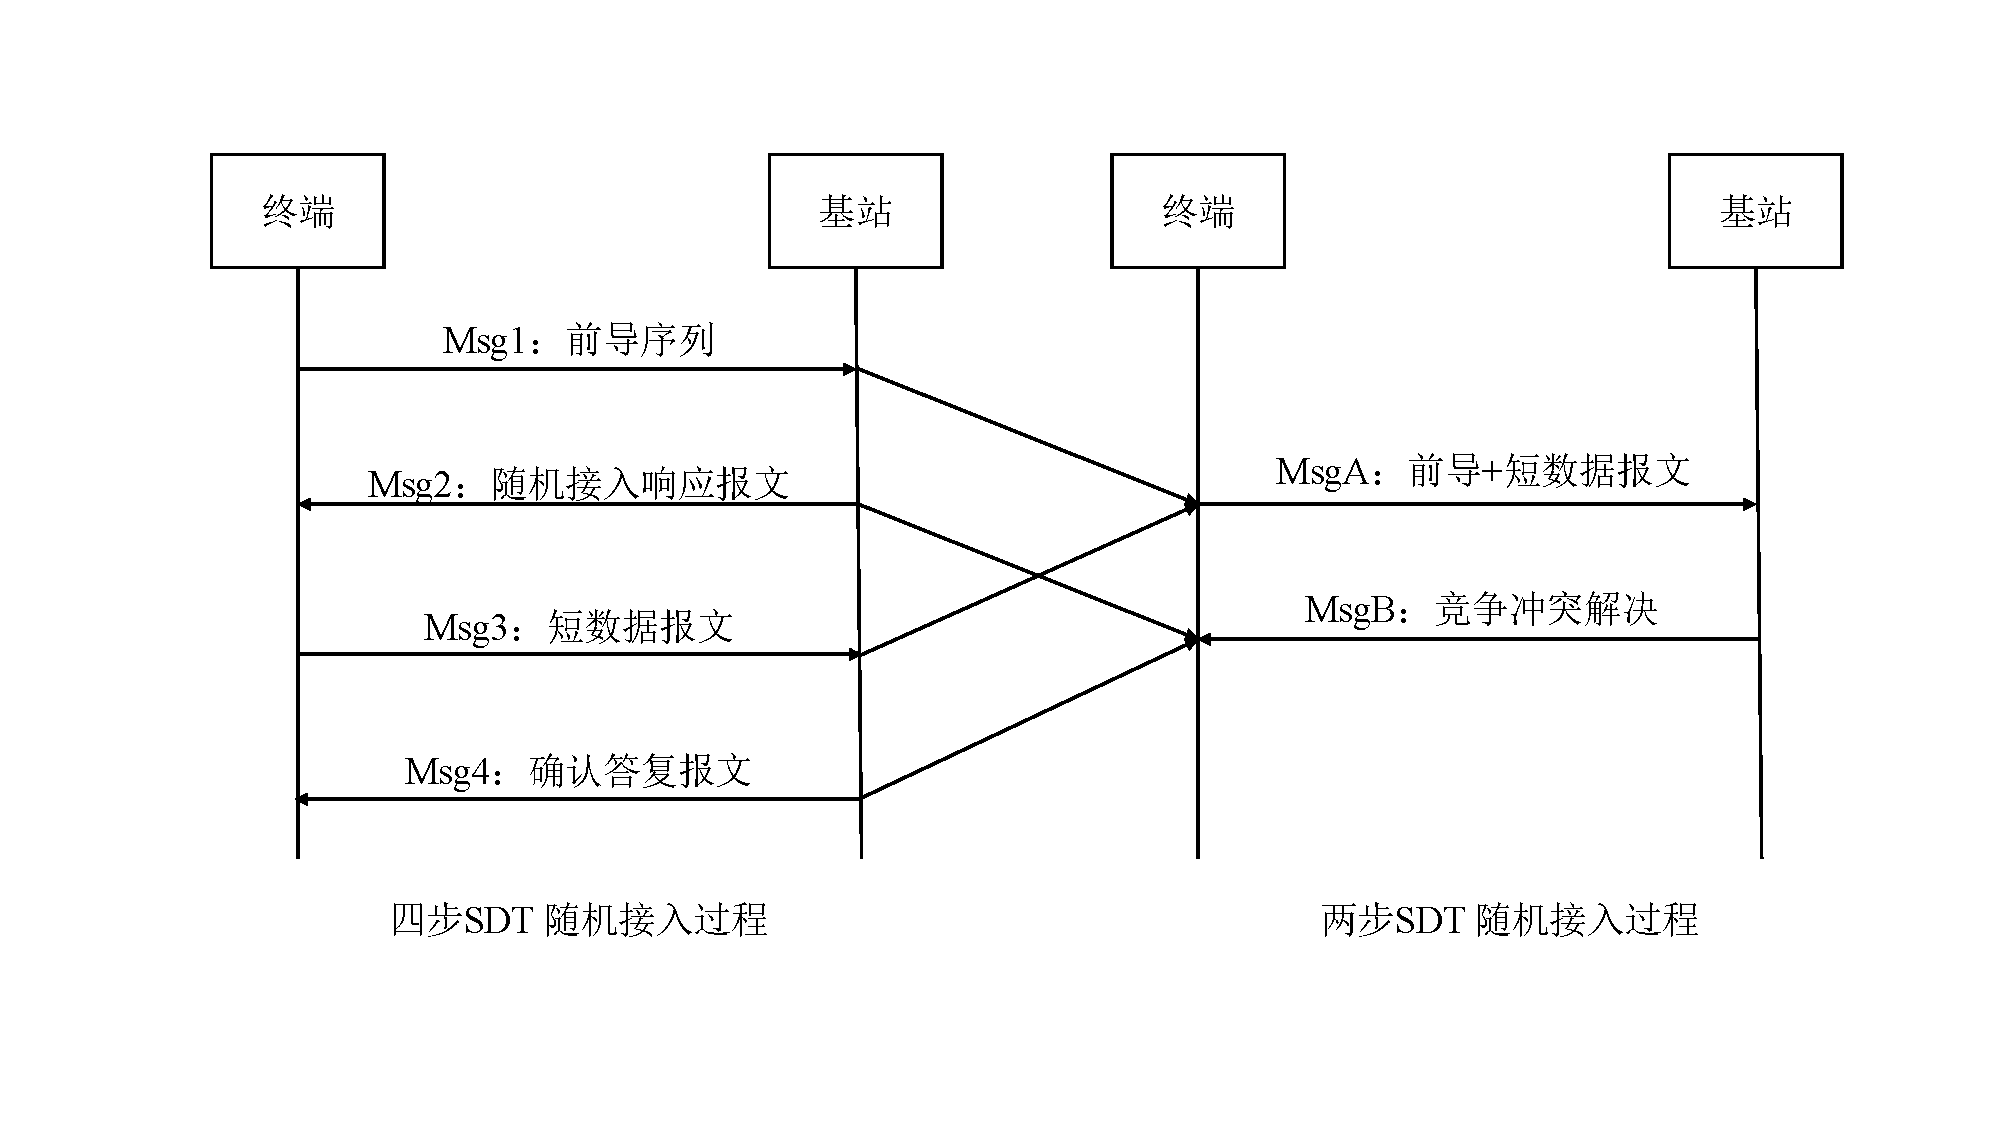
\includegraphics[width=0.95\linewidth]{figure/chap2/5G NR SDT标准随机接入过程.pdf}
	\caption{5G NR 四步/两步 SDT 标准随机接入流程示意图}
	\label{fig:sdt_access}
\end{figure}
在 5G NR 的短数据传输（Short Data Transmission, SDT）场景中，终端在无既有连接状态下，需要首先通过随机接入建立初始通信。在四步SDT标准接入方案中，终端通过发送 Msg1 前导码发起接入，在Msg3传输短报文；而在两步 SDT 标准接入方案中，终端将前导码与数据封装于 MsgA 中一并发送。
尽管信令流程存在差异，但在初始接入阶段，多个终端在离散配置的 PRACH 时隙中独立发起发送请求。两种流程图表示如\ref{fig:sdt_access} 所示。


从 MAC 层视角，每个终端在一个接入机会内仅面临两种决策：发起发送或者保持静默。
该决策可抽象为一次伯努利试验，其发送概率记为 $q \in [0,1]$。不同终端之间的发送行为在统计意义上相互独立。
因此，短报文随机接入在 MAC 抽象层面可视为一种\textbf{时隙化概率竞争机制}，其行为结构与经典的 Slotted Aloha 模型一致，也就是节点在离散时隙中以概率 $q$ 发送，
当且仅当该时隙内恰有一个节点发送时，接入成功。
因此，在不考虑物理层调制、编码等实现细节的前提下，5G 短报文随机接入的接入结构可在理论上等价映射为 Slotted Aloha。

\subsection{NR-U中基于LBT的随机接入过程}
\label{sec:csma_mapping}

在 NR-U（New Radio in Unlicensed Spectrum）场景中，终端在非授权频段发送数据前必须执行Listen-Before-Talk (LBT) 机制。这里假设设备终端已经完成初始接入过程进入到 RRC\_CONNECTED 状态，并且在后续数据传输过程中需要遵守 LBT 规则。根据 3GPP 规范\cite{3gpp38213}，LBT 可分为四种类型（Cat 1–4），其复杂程度与竞争控制能力逐级增强。
\begin{itemize}
    \item Cat 1：无需 LBT；
    \item Cat 2：固定持续时间的信道检测；
    \item Cat 3：随机退避但无指数扩展；
    \item Cat 4：带指数退避的随机退避机制。
\end{itemize}
其中，Cat 4 引入了随机退避与竞争窗口扩展，其结构最接近经典 CSMA/CA。因此，本节重点分析 Cat 4 机制的流程如图\ref{fig:lbt_process}所示，即

\begin{figure}[t]
\centering
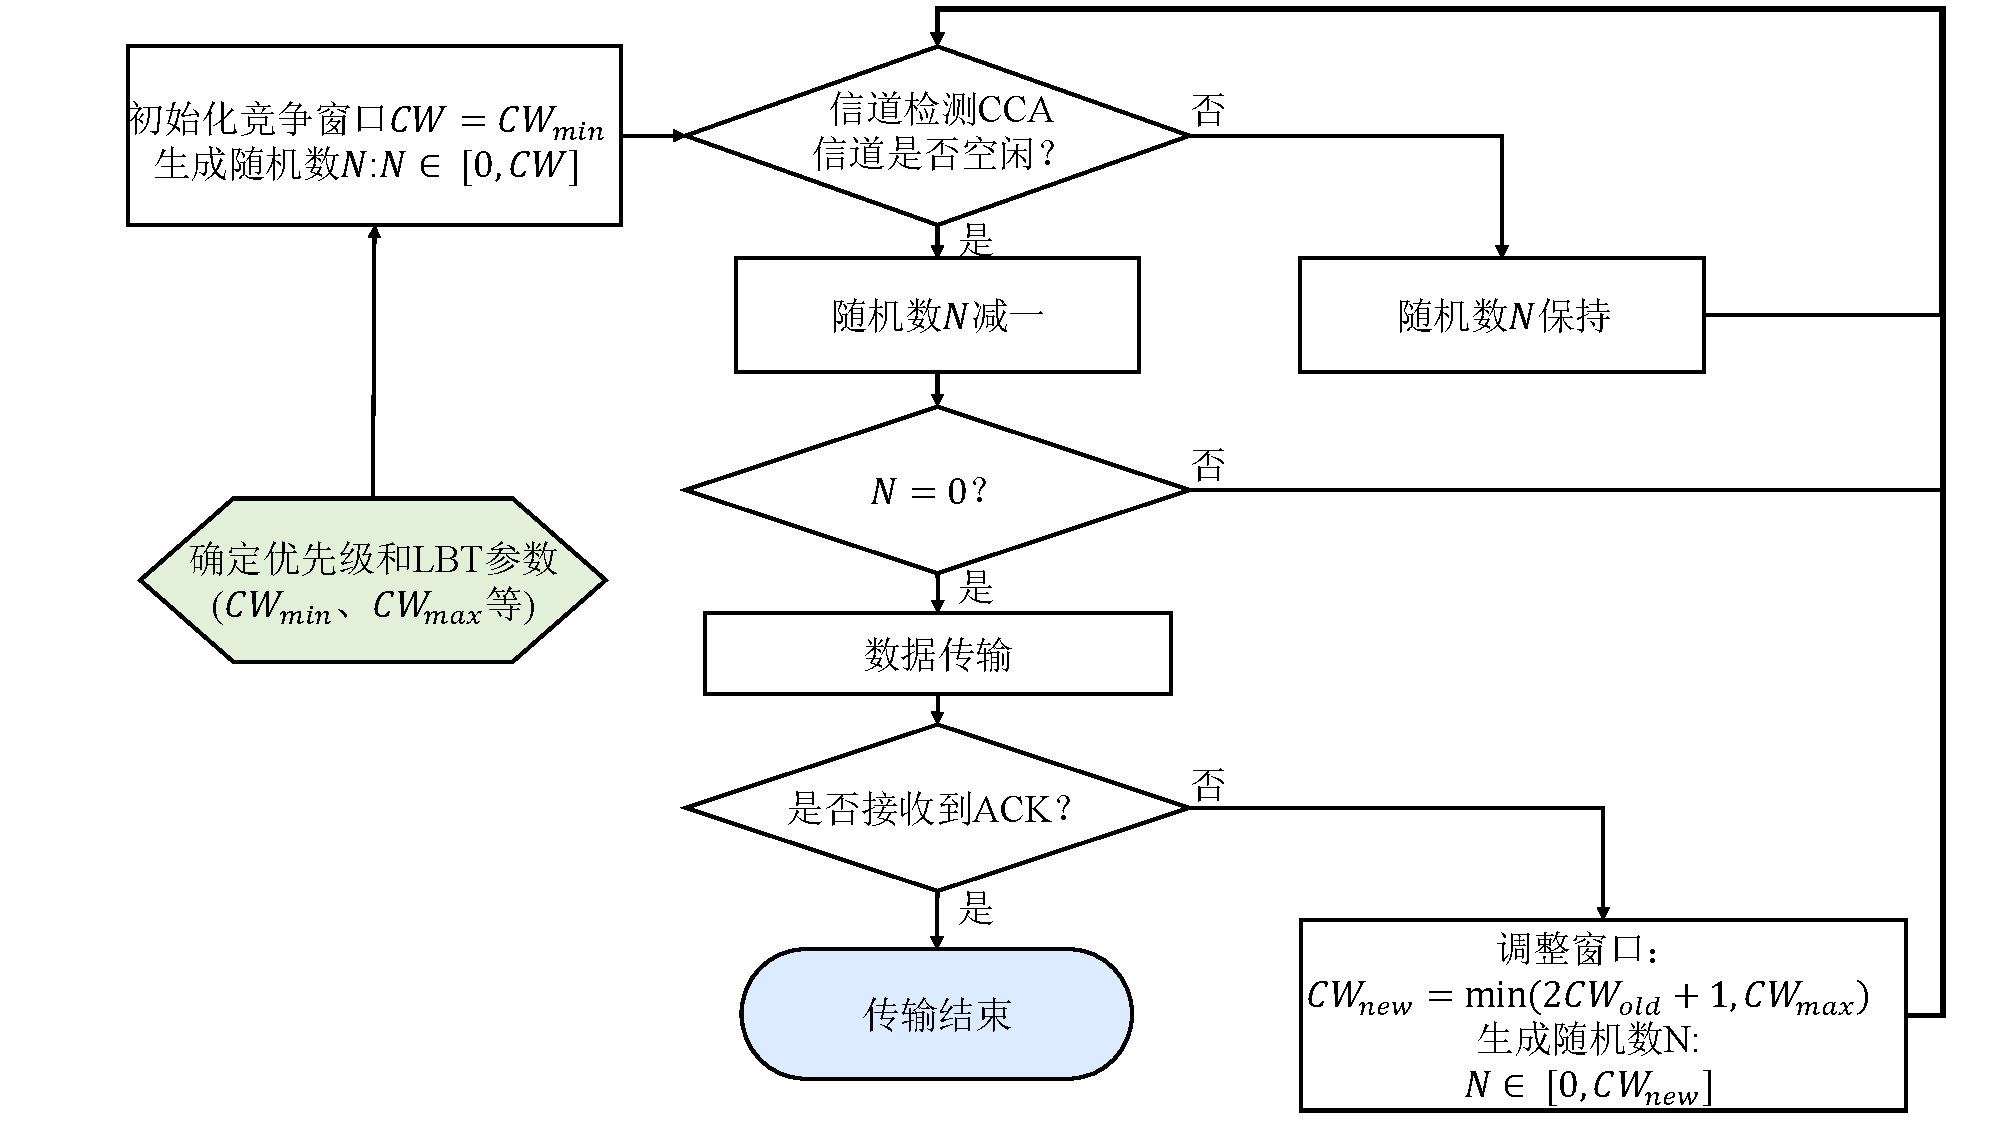
\includegraphics[width=0.9\linewidth]{figure/chap2/5G NR标准LBT过程.pdf}
\caption{NR-U中基于LBT的随机接入流程}
\label{fig:lbt_process}
\end{figure}

\begin{enumerate}[label=\textbf{步骤 \arabic*：}, leftmargin=*, itemsep=1ex]

    \item \textbf{确定信道接入优先级与参数} \\  
    终端在发起传输前，根据业务 QoS 要求选择信道接入优先级类别（Channel Access Priority Class, CAPC）。    每个 CAPC 对应一组预定义的 LBT 参数，包括延迟持续时间参数 $m_p$、竞争窗口最小值 $CW_{\min}$、最大值 $CW_{\max}$，以及最大信道占用时间（Maximum Channel Occupancy Time, MCOT）。
    MCOT 受监管约束限制，用于保证与其他系统的公平共存。

    \item \textbf{竞争窗口更新与退避计数初始化} \\  
    终端根据上一轮传输结果更新竞争窗口 $CW$：
    \begin{itemize}
        \item 若传输成功或为初始传输，则 $CW = CW_{\min}$；
        \item 若传输被判定为失败（例如未收到 HARQ-ACK 或检测到冲突），则
        $CW \leftarrow \min(2CW+1, CW_{\max})$。
    \end{itemize}
    随后在整数区间 $[0, CW]$ 内均匀随机选择退避计数值 $N$。
	
    \item \textbf{执行延迟持续时间（Defer Duration）检测} \\  
    在开始退避计数前，终端必须检测信道在连续时间$T_d = 16\mu s + m_p \times 9\mu s$
    内保持空闲（典型 5 GHz 配置）。若期间检测到信道忙，则需等待信道重新空闲，并重新执行完整的延迟持续时间检测。

    \item \textbf{退避计数与 CCA 时隙监听} \\  
    终端在 $9\mu s$ 的 CCA 时隙上执行退避计数：
    \begin{itemize}
        \item 若信道空闲，则 $N \leftarrow N-1$；
        \item 若信道忙，则冻结计数器，
        待信道重新空闲并重新满足步骤 3 的延迟持续时间要求后恢复倒计时。
    \end{itemize}
    当 $N=0$ 时，终端获得发送机会。

    \item \textbf{数据发送与 MCOT 约束} \\  
    终端在获得信道后进行数据传输，
    传输持续时间不得超过该 CAPC 对应的 $T_{mcot,p}$。
    传输结束后，
    根据成功或失败结果更新 $CW$，
    为下一次接入做准备。
\end{enumerate}

从接入机制的本质出发，Type 4 LBT 与经典 CSMA/CA 在 MAC 层具有一一对应的竞争逻辑：二者均遵循“先侦听、后发送”的信道占用原则，均通过随机退避计数分散并发发送时机，并在失败后通过竞争窗口扩展抑制后续冲突概率。因而，在以时隙化 CCA、理想碰撞信道和饱和/非饱和队列业务为前提的理论分析框架下，NR-U 的 LBT 过程可等效抽象为 CSMA 型随机接入网络。该抽象保留了影响吞吐量、时延与公平性的主要竞争行为，同时忽略物理层调制、频谱监管细节与跨系统共存策略等次要差异，因此可作为后续 CSMA 网络建模与性能推导的合理基础。

\section{连续传输机制的基本原理}
\label{sec:continuous_transmission_principle}



传统随机接入协议（如 Aloha 与 CSMA）通常采用一次竞争、发送一个数据包的工作方式：节点每完成一次发送后都需释放信道，并重新进入竞争或退避过程。该机制在中高负载下会反复消耗竞争时隙，使大量时间开销停留在侦听、退避与握手环节而非有效载荷传输。为降低这部分重复开销，本文引入连续传输（Successive Transmission, ST）机制：节点一旦竞争成功并完成队首分组发送，可在满足协议约束的条件下继续发送后续缓存分组，直到队列清空或触发释放条件，再重新进入竞争过程。

如图\ref{fig:ra_vs_st} 所示，传统机制下每个数据包通常对应一次独立竞争，竞争开销与数据包数量近似线性增长；而在 ST 机制下，一次竞争成功可支撑多个数据包连续发送，使竞争开销由“按包重复发生”转变为“按轮次分摊”。因此，ST 的核心增益在于降低单位数据包的平均竞争开销（Contention Overhead），并在不改变随机接入基本竞争框架的前提下提升有效信道利用率与系统吞吐效率。
\begin{figure}[t]
	\centering
	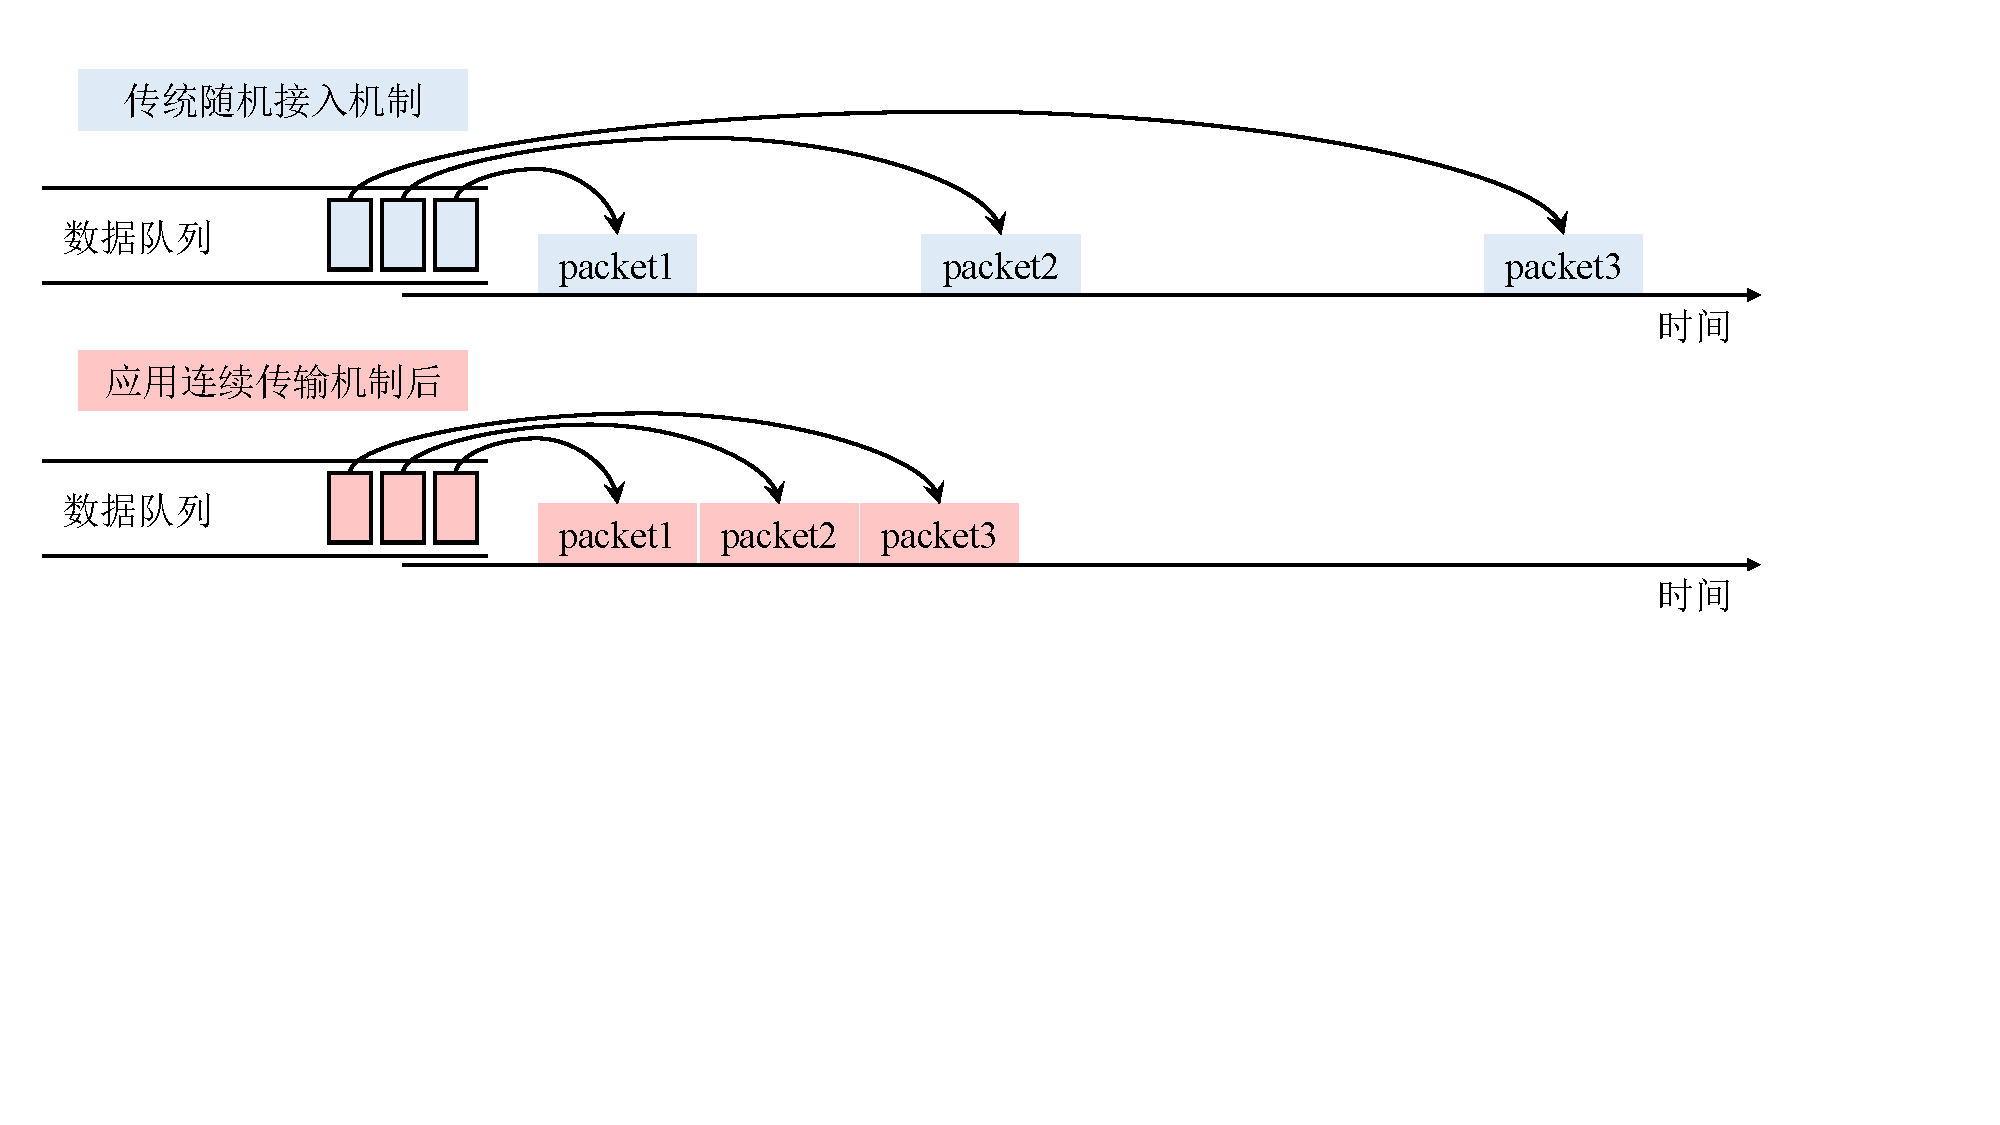
\includegraphics[width=0.95\linewidth]{figure/chap2/连续传输机制对比图.pdf}
	\caption{传统随机接入与连续传输机制的对比图}
	\label{fig:ra_vs_st}
\end{figure}
\section{通用系统场景与模型假设}
\label{sec:general_system_model}


为构建具有普适性与可扩展性的理论分析框架，并为后续章节中不同接入机制（SAST 与 CSMAST）的性能比较提供统一分析基准，本文首先建立一个抽象化的上行随机接入网络系统模型。在保证物理拓扑结构一致性的前提下，通过对节点行为机制进行差异化建模，实现对多种接入范式的统一刻画与对比分析。

本章节考虑一个包含 $n$ 个同质终端节点（User Equipment, UE）和一个中心基站（Base Station, BS，亦作为统一接收机）的上行通用无线随机接入系统，如图~\ref{fig:system_model} 所示。所有节点通过共享无线信道向同一接收机发送数据，接收机负责信号接收、译码与反馈。系统中仅接收机设计接收结构，而节点之间不存在显式协调或直接通信机制。
\begin{figure}[t]
	\centering
	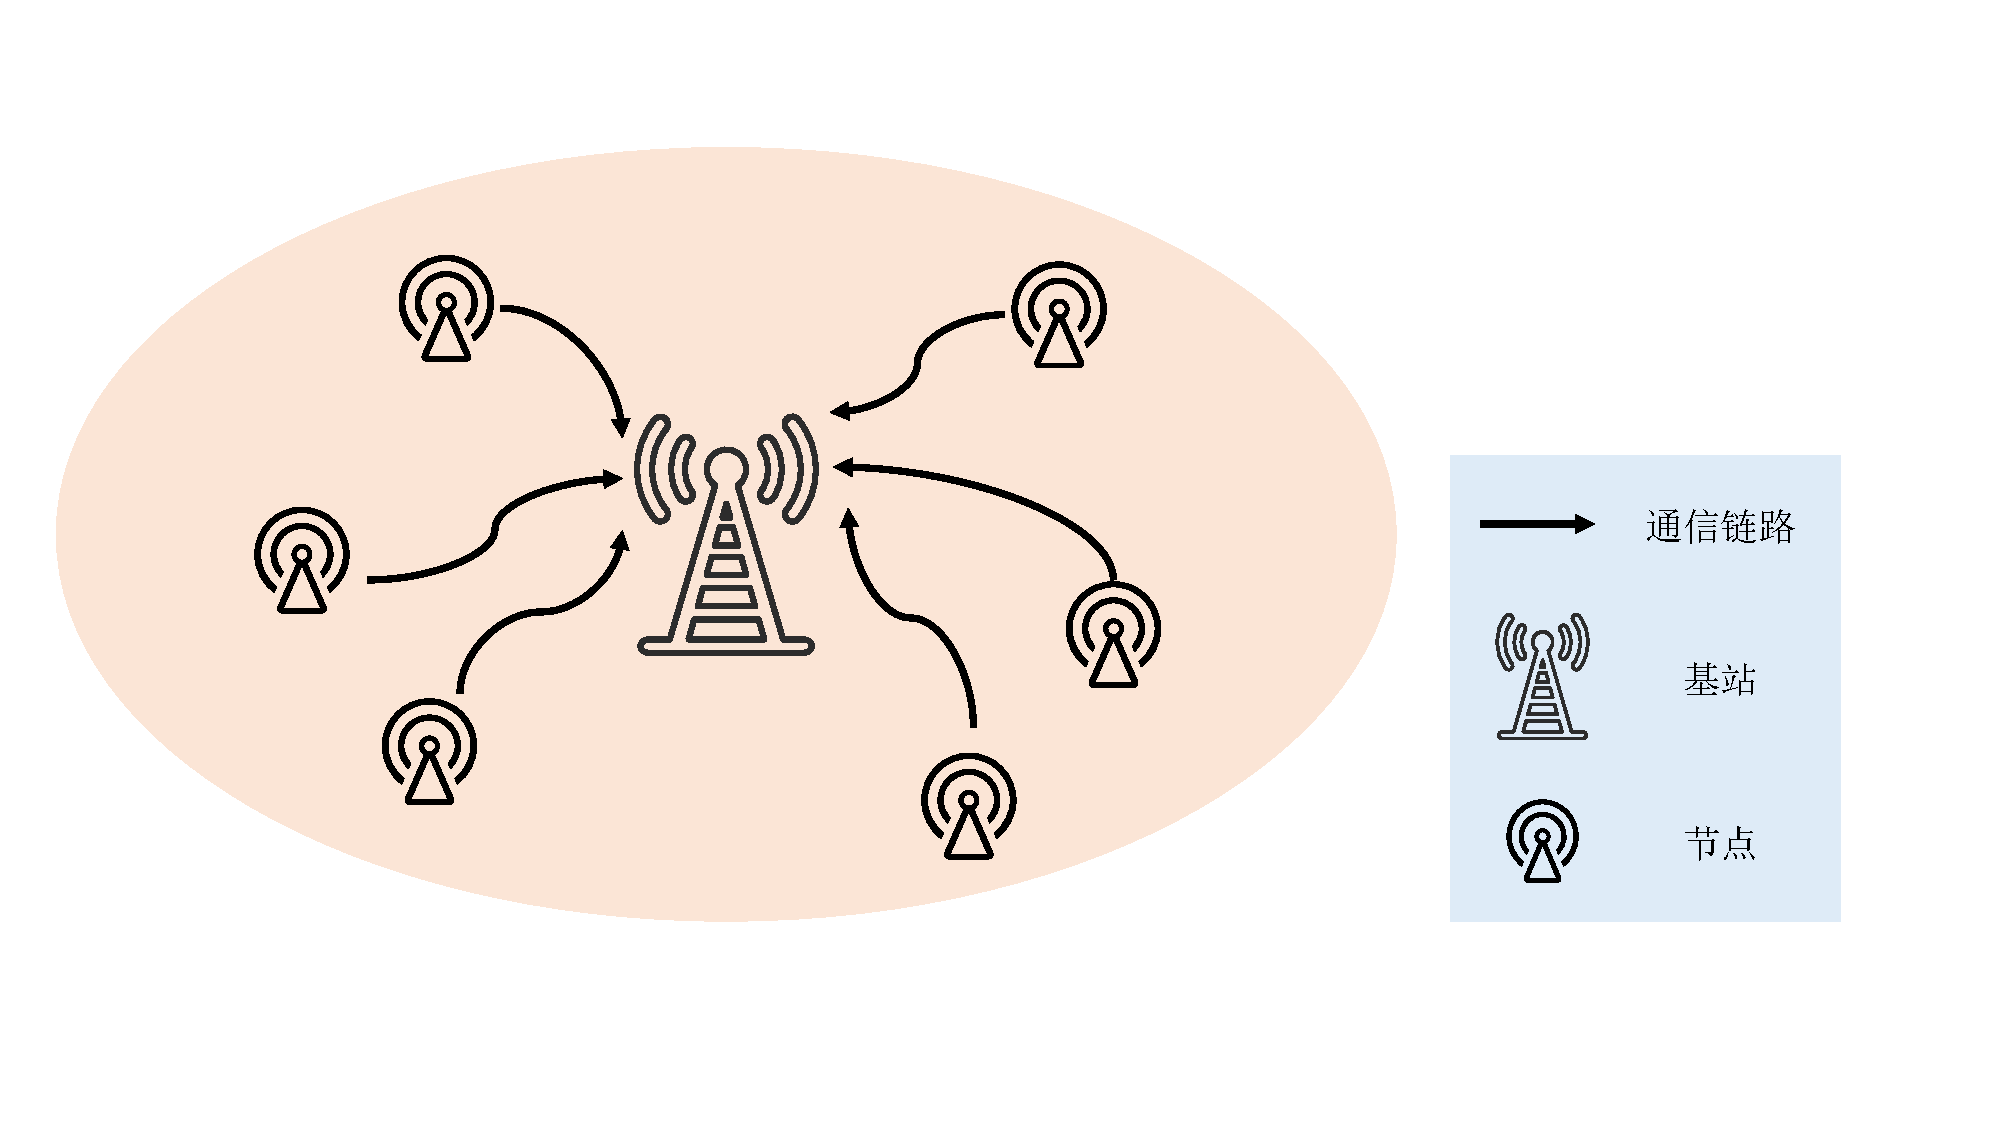
\includegraphics[width=0.9\linewidth]{figure/chap2/通用系统场景.pdf}
	\caption{通用系统场景示意图}
	\label{fig:system_model}
\end{figure}

需要特别说明的是，尽管后续各章节的分析重点不同，但“接收机—节点”物理拓扑关系在全文中保持一致。不同章节之间的差异主要体现在节点侧接入策略与控制逻辑的设计，而非系统结构本身的改变。具体而言：

\begin{itemize}
	\item 在第~\ref{chapter3: SAST }章中，基站主要承担集中接收与反馈功能，终端节点的行为建模侧重于概率发送与连续传输的传输策略，系统分析聚焦于基于连续传输的时隙 ALOHA 机制的性能刻画；
	
	\item 在第~\ref{chapter4: CSMAST }章中，基站仍作为统一接收实体，而终端节点行为进一步扩展为“侦听—退避—发送”的竞争式接入过程，系统模型引入载波监听机制和连续传输，用以刻画 CSMAST 协议的动态行为和性能分析；
	
	\item 在第~\ref{chapter5: ai_selector}章中，在保持统一拓扑结构不变的前提下，研究重点转向不同协议与参数组合下的性能评估与接入协议智能切换机制。此时节点配备有多重接入协议策略，其具体接入行为被抽象为可切换的策略集合，分析核心从单一接入协议到多接入协议策略集合的性能。
\end{itemize}

在上述通用系统场景框架下，具体系统假设如下：

\begin{itemize}
	\item \textbf{网络拓扑与流量模型}：网络由 $n$ 个统计特性相同的同质节点组成。各节点的数据包到达过程独立且同分布（i.i.d.）。
	
	为了便于第\ref{chapter3: SAST }、\ref{chapter4: CSMAST }章的排队论解析推导，本文在\textbf{理论分析模型}中假设各节点的包到达过程均服从参数为 $\lambda$ （单位：包/时隙）的伯努利过程，即每个节点在每个时隙有新数据包到达的概率为 $\lambda$，且不同时隙的到达事件相互独立，因而系统的总到达率为 $\hat{\lambda} = n\lambda$。这一简化假设使得系统动态可精确刻画为离散时间马尔可夫链，便于应用休假排队理论进行闭式求解。
	
	然而，现实通信场景中的到达过程通常具有显著的非平稳性与多尺度统计特征。为与第\ref{chapter5: ai_selector}章保持一致，本文在仿真与业务建模中采用统一流量特征向量
	$\mathbf{x}_{\text{traffic}}=[\hat{\lambda},\ \mathrm{BI}_{\mathrm{net}},\ \mathrm{BI}_{\mathrm{node}},\ \Psi_{\mathrm{net}},\ \Psi_{\mathrm{node}}]^{\top}$，
	其中网络突发度与网络周期性强度分别定义为
	$\mathrm{BI}_{\mathrm{net}}=\frac{\mathrm{ID}_{\mathrm{net}}-1}{\mathrm{ID}_{\mathrm{net}}+1}$、
	$\mathrm{ID}_{\mathrm{net}}=\frac{\mathrm{Var}(X(t))}{\mathbb{E}[X(t)]}$，以及
	$\Psi_{\mathrm{net}}=\max_{1\le\tau\le\tau_{\max}}\frac{R(\tau)}{R(0)}$。
	在该定义下，本文采用与第\ref{chapter5: ai_selector}章一致的三类典型流量形态：
	\begin{itemize}
		\item \textbf{均匀到达场景（U）}：$\mathrm{BI}_{\mathrm{net}}\approx 0$ 且 $\Psi_{\mathrm{net}}\approx 0$，对应近似泊松到达；
		\item \textbf{突发到达场景（B）}：$\mathrm{BI}_{\mathrm{net}}\in[0.3,0.7]$ 且 $\Psi_{\mathrm{net}}\in[0,0.2]$，采用 MMPP/批量到达过程刻画事件驱动型集中上报；
		\item \textbf{周期到达场景（P）}：$\mathrm{BI}_{\mathrm{net}}\in[-0.5,-0.2]$ 且 $\Psi_{\mathrm{net}}\in[0.6,0.9]$，刻画规则采样或同步上报业务。
	\end{itemize}
	
	上述流量特征的完整定义与计算公式见第\ref{chapter5: ai_selector}章表~\ref{tab:traffic_feature_def}，具体参数配置与采样策略见该章仿真实验部分。
	
	\item \textbf{时隙结构与同步}：系统采用离散时间模型，时间轴被划分为连续且等长的时隙（Time Slot）。时隙长度被标准化为传输一个固定长度数据包所需的时间。系统假定所有节点保持严格的时钟同步，因此所有数据包的传输只能在每个时隙的起始时刻发起。
	
	\item \textbf{信道模型}：假设信道为理想无噪声信道，采用标准的碰撞信道模型（Collision Model）。当且仅当一个时隙内只有一个节点进行传输时，接收机才能成功解码数据包；若多个节点在同一时隙并发传输，则发生信号叠加导致碰撞，所有涉及的数据包均传输失败且无法恢复。
	
	\item \textbf{反馈机制}：假设基站提供完美且即时的反馈。节点在每个传输时隙结束时，能够立即通过 ACK（确认）或 NACK（否定确认）信令获知该次传输是否成功。分析中忽略反馈信道的传输错误及传播延迟。
	
	\item \textbf{数据包与信令开销}：假设系统中传输的所有数据包具有固定的长度，且完整占用一个时隙。相比之下，控制信令（如 ACK/NACK）的数据量极小，其传输时间在分析中被视为瞬时完成，或已包含在时隙的保护间隔（Guard Interval）内，不额外占用数据传输资源。
	
	\item \textbf{缓存队列与网络状态}：每个节点配备容量无限大的缓冲区（Infinite Buffer），数据包在缓冲区中遵循先进先出（FIFO）原则。在此假设下，数据包不会因缓存溢出而丢失，但可能会在队列中积压。根据节点缓存的积压情况，我们将网络运行状态划分为两类用于后续分析：
	\begin{itemize}
		\item \textbf{饱和状态（Saturated State）}：假设节点缓存始终非空（即 $p_{ne}=1$），节点始终有数据包待传。此状态用于推导系统的理论吞吐量极限。
		\item \textbf{非饱和状态（Unsaturated State）}：节点缓存可能为空（即 $p_{ne} < 1$）。此状态更符合实际流量场景，用于评估系统的稳态时延与实际吞吐量。
	\end{itemize}
\end{itemize}

基于上述通用假设，后续章节将在统一场景下展开递进分析：第~\ref{chapter3: SAST }章聚焦 SAST 机制下 Aloha 型接入的吞吐量与时延等性能特性，第~\ref{chapter4: CSMAST }章分析 CSMAST 机制下的性能边界；在此基础上，第~\ref{chapter5: ai_selector}章进一步面向多业务与动态负载环境，综合吞吐量、时延、公平性与信令开销等指标，研究多协议智能切换与参数自适应优化问题。

\section{基于休假排队理论的分析方法}
\label{sec:vacation_queuing_theory}

在引入连续传输机制后，节点与信道状态呈现出显著的“服务—休假”交替特征：当节点竞争成功并占用信道时，系统进入忙期；当节点因退避、碰撞重传或队列暂空而未进行有效传输时，系统进入休假期。该过程具有明显的循环更新结构，使得仅依赖低维状态转移的传统马尔可夫描述在表达能力与可解性之间面临权衡。为此，本文采用离散时间休假排队理论（Discrete-time Vacation Queuing Theory）作为后续理论推导的统一分析框架。

在该框架中，复杂竞争行为被重构为忙期长度与休假期长度两类随机过程的耦合分析问题。前者刻画一次成功接入后连续服务的持续能力，后者刻画节点在非服务阶段经历的等待、退避与重试代价。基于这一分解，系统关键性能可由可解释的统计量统一表征：忙期主导有效数据服务能力，休假期主导竞争开销与等待时延。

进一步地，本文从“信道视角”与“节点视角”两个层面开展分析。信道视角关注聚合流量下忙期—休假期交替规律，以推导系统吞吐量及其稳定工作区间；节点视角关注单节点队列在休假期内的积压增长与忙期内的服务消减，结合概率生成函数（PGF）及其变换性质求取队列稳态分布，并据此利用 Little 定律得到平均时延表达式。由此建立的分析路径可在统一数学框架下同时覆盖 Aloha 与 CSMA 两类机制，并为第~\ref{chapter3: SAST }章、第~\ref{chapter4: CSMAST }章及第~\ref{chapter5: ai_selector}章中的性能推导、对比与策略优化提供一致且可复用的理论基础。

\section{关键性能指标定义}
\label{sec:performance_metrics}

为了全面评估所提机制的有效性，并与现有标准方案进行公平对比，本章统一定义以下关键性能指标，涵盖效率、时延、公平性与开销四个维度。

\subsection{吞吐量指标}

吞吐量是衡量系统有效传输能力的核心指标,本文细分为接入吞吐量与数据吞吐量两类：

\begin{itemize}
	\item \textbf{接入吞吐量（Access Throughput, $S_a$）}：定义为单位时间（时隙）内成功传输的队首数据包（Head-of-Line Packet）或接入请求的平均数量，单位为包/时隙。该指标反映了系统处理并发接入请求的能力，对应于信道视角下的成功接入事件率。在理论分析中，接入吞吐量可通过竞争成功概率与节点非空概率的乘积计算：
	\begin{equation}
	S_a = n \cdot p_{tx} \cdot (1 - p_{tx})^{n-1} \cdot p_{ne}
	\end{equation}
	其中 $n$ 为节点数，$p_{tx}$ 为发送概率，$p_{ne}$ 为节点非空概率。
	
	\item \textbf{数据吞吐量（Data Throughput, $S_d$）}：定义为单位时间内信道成功传输的所有数据包（包含连续传输的后续包）的平均数量，单位为包/时隙。该指标衡量系统的有效负载传输效率。对于引入连续传输的系统，数据吞吐量显著高于接入吞吐量，两者之比反映了连续传输的增益：
	\begin{equation}
	\text{Throughput Gain} = \frac{S_d}{S_a}
	\end{equation}
\end{itemize}

\subsection{时延指标}

时延直接影响用户体验与服务质量，本文区分接入时延与端到端数据包时延：

\begin{itemize}
	\item \textbf{接入时延（Access Delay, $D_a$）}：定义为一个数据包从到达队首（成为HoL包）开始，到其成功被基站接收所经历的时间，单位为时隙。该指标主要体现竞争接入的等待成本，包含碰撞重传与退避等待时间。在休假排队模型中，接入时延等于休假期长度的期望值。
	
	\item \textbf{数据包时延（Packet Delay, $D_p$）}：定义为数据包从生成时刻进入缓存队列，直到被成功传输完毕离开系统的全过程时延，单位为时隙。该指标包含排队等待时间（队列中排在该包前面的所有包的服务时间）与接入服务时间（该包自身的接入与传输时间），直接反映端到端用户体验。根据Little定律，平均数据包时延可表示为：
	\begin{equation}
	D_p = \frac{E[Q]}{\lambda_{eff}}
	\end{equation}
	其中 $E[Q]$ 为平均队列长度，$\lambda_{eff}$ 为有效到达率。
\end{itemize}

\subsection{公平性指标}

在多用户竞争环境中，资源分配的公平性直接影响系统的稳定性与用户满意度。本文采用Jain公平性指数（Jain's Fairness Index, JFI）作为统一的公平性度量：

\begin{equation}
\text{JFI} = \frac{\left(\sum_{i=1}^{n} x_i\right)^2}{n \cdot \sum_{i=1}^{n} x_i^2}
\end{equation}

其中 $x_i$ 表示第 $i$ 个节点在观测时间窗口内获得的资源份额（可以是成功传输的数据包数量、占用的时隙数、或获得的吞吐量）。JFI的取值范围为 $[1/n, 1]$，其中 $1/n$ 表示最不公平情况（仅一个节点占用全部资源），$1$ 表示完全公平（所有节点获得相同资源）。

在本文的分析中，我们特别关注\textbf{短期公平性（Short-term Fairness）}，即在数十至数百个时隙的观测窗口内的资源分配公平性。这是因为：\textbf{（1）}连续传输机制允许单个节点连续占用信道，可能导致短期内的不公平现象；\textbf{（2）}实时业务（如VoIP、视频流）对短期时延抖动敏感，长期统计公平性无法反映瞬时服务质量；\textbf{（3）}短期公平性能够捕捉协议在动态流量变化下的瞬态行为。第\ref{chapter4: CSMAST }章和第\ref{chapter5: ai_selector}章将采用滑动窗口法计算不同时间尺度下的JFI，以评估SAST与CSMAST机制在公平性方面的权衡。

\subsection{信令开销指标}

控制信令开销是随机接入系统的重要成本，直接影响能量效率与频谱利用率。本文统一采用以下度量方式：

\begin{itemize}
	\item \textbf{信令吞吐比（Signaling-to-Throughput Ratio, STR）}：定义为每成功传输一个有效数据包所需消耗的平均信令比特数，单位为比特/包。对于标准随机接入方案，信令包括前导码（Preamble）、握手消息（Handshake）、反馈信令（ACK/NACK）等。STR越低，说明系统的信令效率越高。在第\ref{chapter3: SAST }章的理论分析中，STR可表示为：
	\begin{equation}
	\text{STR} = \frac{C_{pre} + C_{hs} + C_{ack} \cdot E[N_{tx}]}{L_{data}}
	\end{equation}
	其中 $C_{pre}$、$C_{hs}$、$C_{ack}$ 分别为前导码、握手包、反馈信令的比特开销，$E[N_{tx}]$ 为平均传输次数（含重传），$L_{data}$ 为数据包长度。
	
	\item \textbf{归一化信令开销（Normalized Signaling Overhead, $S$）}：定义为信令开销与有效数据吞吐量的比值，量纲为无量纲数。该指标在第\ref{chapter5: ai_selector}章的协议选择与效用优化中作为惩罚项使用：
	\begin{equation}
	S = \frac{\text{Total Signaling Bits per Time Unit}}{\text{Data Throughput} \times L_{data}}
	\end{equation}
	归一化信令开销 $S$ 等价于每比特有效数据传输所需的信令比特数，反映了系统的频谱效率。在效用函数设计中，通过调节信令开销的权重因子，可以在吞吐量与能效之间实现灵活的权衡优化。
\end{itemize}

\textbf{度量单位的统一说明}：本文在理论分析中通常以"次数"（如接入次数、重传次数）或"归一化时隙数"作为信令开销的基本单位，便于解析求解；在仿真验证与实际对比中，则采用"比特数"或"归一化比特数"作为统一度量单位，以便与5G等标准方案进行公平对比。两种度量方式可通过信令包的固定长度进行线性转换。

通过上述四类指标的综合评估，本文能够在效率、时延、公平性与开销等多个维度全面刻画所提连续传输机制的性能特征，并为后续章节的理论分析与仿真实验提供统一的评价基准。

        \newclearpage
        \chapter{面向 Aloha 协议的连续传输机制设计与性能分析}
\label{chapter3:SAST}

上一章分析了 5G 随机接入标准框架。尽管其包含复杂的信令与协议过程，但在 2 步小数据传输场景下，可将接入过程抽象为时隙 Aloha 模型。基于此，本章回到抽象模型，在统一假设下分析接入竞争与连续传输机制。在此基础上，提出连续传输增强的时隙 Aloha 机制，即 SAST ，并依次给出机制流程、休假排队建模以及吞吐量与时延性能分析。 

\section{SAST系统模型与机制描述}
\label{sec:sast_system_model}

本章所研究的 SAST 网络环境遵循~\ref{sec:general_system_model}~节定义的通用系统模型。具体而言，考虑由 $n$ 个同质节点和单个接收机构成的分布式时隙 Aloha 网络，节点流量服从伯努利到达，信道采用碰撞模型，且具备即时无误的确认或否定确认反馈机制。

SAST 协议的核心策略可以概括为一次接入、连续占用，可打破传统 Aloha 协议中每发送一个数据包都需重新竞争的低效模式。具体而言，当节点缓存非空时，首先以概率 $q \in [0,1]$ 参与随机竞争并传输队首数据包。若接收机成功解码该数据包，则回复确认消息，节点随即进入连续传输阶段；若发生碰撞或解码失败，则回复否定确认消息，节点在下一时隙重新以概率 $q$ 尝试接入。一旦队首数据包成功传输，该节点便可视为获得了短时信道占用权。在后续若干时隙内，该节点不再进行随机退避，而是以概率 1 连续发送缓存中的剩余数据包，直到缓存清空或发生信道碰撞。

为了直观展示这一过程，图~\ref{fig:two_node_sast} 以两个节点为例，描绘了 SAST 网络中典型的竞争、连续传输及中断过程：
\begin{figure}[t]
	\centering
	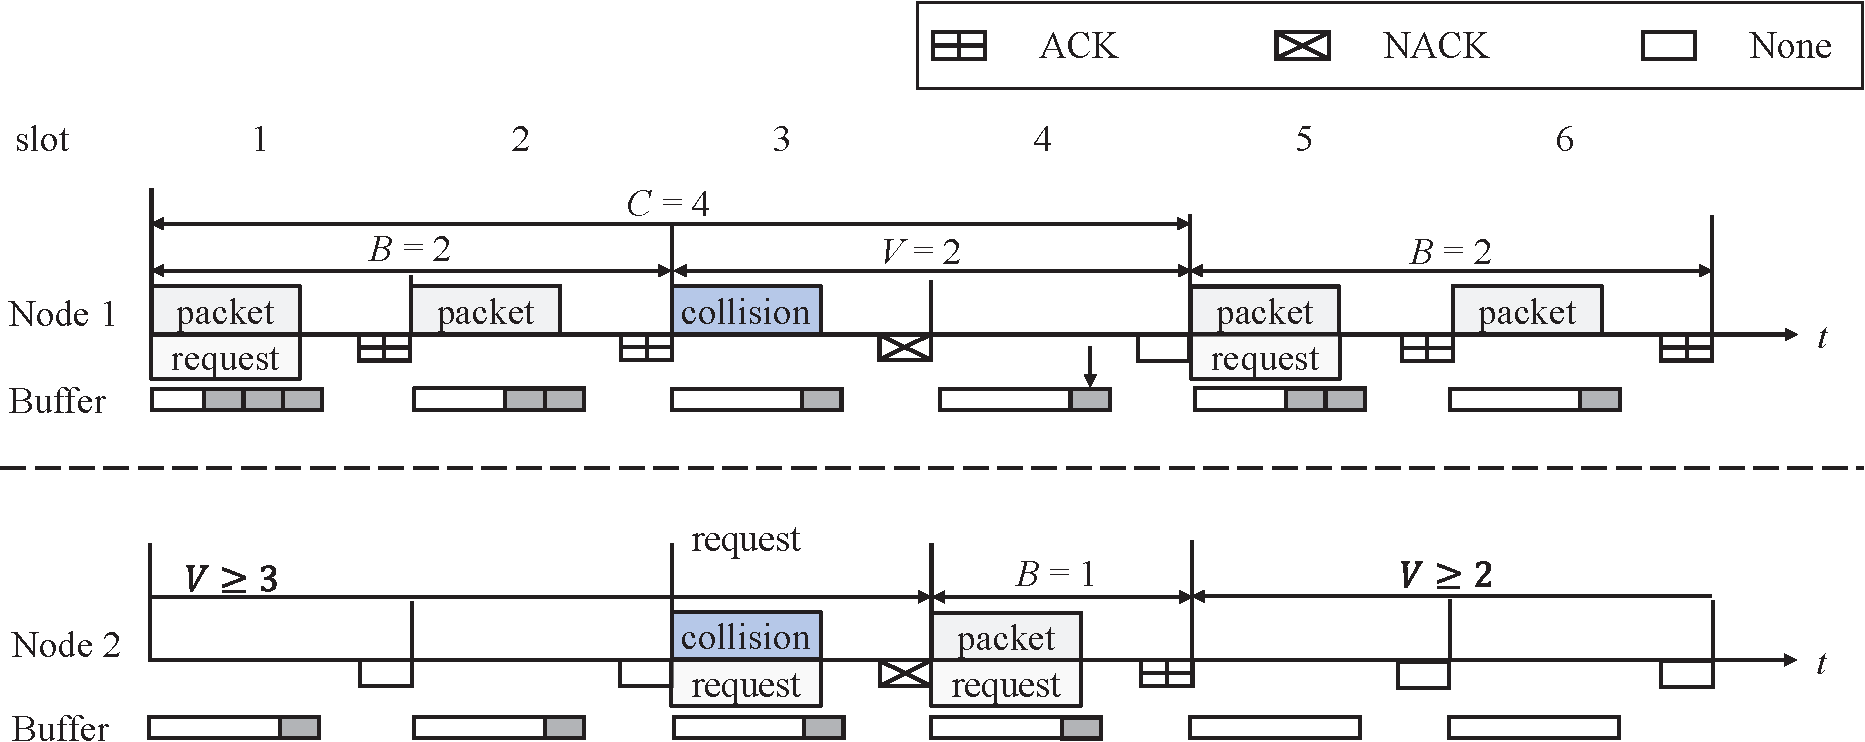
\includegraphics[width=0.9\textwidth]{figure/chap3/two_node_sast.pdf}
	\caption{两节点 SAST 网络时序示意图}
	\label{fig:two_node_sast}
\end{figure}
\begin{description}
	\item[时隙 1 （初始接入）：] 节点 1 以概率 $q$ 成功发送队首数据包，而节点 2 保持静默。节点 1 收到确认反馈后进入连续传输状态。
	\item[时隙 2 （连续传输）：] 节点 1 无需再次竞争，直接以概率 1 发送缓存中的第二个数据包并成功。
	\item[时隙 3 （碰撞中断）：] 节点 1 试图发送第三个数据包。与此同时，节点 2 恰好到达新数据包并以概率 $q$ 发起队首包传输。两者信号叠加引发碰撞，基站回复否定确认。此次碰撞强制中止了节点 1 的连续传输过程，使其退回常规竞争状态。
	\item[时隙 4 （重新竞争）：] 网络恢复到无节点占用的状态。节点 1 和节点 2 重新参与信道竞争，此时节点 2 以概率 $q$ 成功抢占信道发送队首包，而节点 1 保持静默。
\end{description}

需要特别指出的是，本章所提出的 SAST 机制在思想上虽与传统基于连接的 Aloha 或 5G 中的免调度均体现出一定的连续占用特征，但在设计范式存在本质区别。现有机制通常依赖显式预约或连接建立过程来实现信道的持续占用，SAST 采用的是一种隐式预留策略：节点无需发送专门的 RTS/RRC 等额外控制信令，而是用 5G 标准中的 MsgA 报文进行竞争；一旦基站成功解码并反馈 MsgB，后续信道占用通过连续发送数据报文自然延续，该过程是不改变现有分布式接入架构与帧结构的。
为避免与其他 Aloha 类协议混淆，这里从机制实现角度对三类 Aloha 协议作简要总结，如表~\ref{tab:aloha_compare} 所示。

\begin{table}[htbp]
\centering
\caption{SA、CBA 与 SAST 机制的核心特性对比}
\label{tab:aloha_compare}
\renewcommand{\arraystretch}{1.3} 
\begin{tabular}{l c c c}
\toprule
\textbf{对比维度} & \textbf{SA} & \textbf{CBA} & \textbf{SAST（本文）} \\
\midrule
接入机制 & 逐包独立竞争 & 显式信令预约 & 隐式预留 (复用 MsgA) \\
连续传输 & 不支持 & 静态配置 (固定 $M$) & 动态自适应 (队列驱动) \\
释放条件 & 单包传毕即放 & 预留期满释放 & 队列清空或遭遇碰撞 \\
连接管理 & 无连接态 & 需建立与维护连接 & 无连接态 \\
信令开销 & 基础反馈 & 高 (需控制信令交互) & 基础反馈 \\
中断机制 & 不适用 & 预留期内不可打断 & 碰撞即时中断并退避 \\
\bottomrule
\end{tabular}
\end{table}

\section{基于休假排队理论的系统建模}
\label{sec:sast_queuing_model}

为深入量化分析 SAST 机制的性能，本节引入离散时间休假排队理论\cite{2021_Huang}，分别从节点和信道两个互补视角对系统行为进行建模。这种建模方法能够有效地将节点的数据包到达过程与信道的传输竞争过程解耦，从而通过分析忙期与假期的统计特性推导系统的吞吐量与时延性能。

%\subsection{节点视角的休假队列模型}
\label{subsec:node_perspective}

从节点视角出发，节点在长期运行过程中可抽象为两个交替出现的阶段，即节点忙期 $B$ 与节点假期 $V$。其中，忙期 $B$ 指节点成功占用信道后以连续传输方式发送数据包的时间段。由于本章采用离散时隙模型，并以成功接入作为忙期触发事件，因此忙期 $B$ 的计数从队首数据包成功传输所在的时隙开始，从而 $B\ge 1$。随后节点进入连续传输阶段，在后续时隙中以概率 1 发送队列中的剩余数据包，直至缓存清空或发生碰撞时结束。假期 $V$ 则表示节点未能完成成功数据传输的时间段，主要包括三类情形：缓存为空、缓存非空但未发起接入，以及发起接入但发生碰撞。此外，定义节点周期 $C$ 为相邻两次忙期起始时刻之间的时间间隔，因此有 $C = B + V$。

从信道视角来看，其运行状态同样呈现出周期性交替特征。定义信道忙期 $B_c$、信道假期 $V_c$ 和信道周期 $C_c$。其中，信道忙期 $B_c$ 指信道被任意一个节点成功占用并进行数据传输的时间段，信道假期 $V_c$ 指信道上没有数据包被成功解码的时间段，即信道处于空闲状态或发生碰撞，信道周期 $C_c$ 为两个连续信道忙期起始点之间的时间间隔，即 $C_c = B_c + V_c$。
值得注意的是，由于信道忙期 $B_c$是由任意一个节点的成功接入所触发的，因此信道忙期 $B_c$ 的概率分布与单个节点的忙期 $B$ 完全一致。为简化符号，后续分析中将统一使用 $B$ 来表示忙期。

基于上述休假排队模型的符号定义，网络的接入吞吐量 $\lambda^a_{out}$和数据吞吐量 $\lambda^d_{out}$可由信道周期的统计特性推导定义。
由于在一个信道周期 $C_c$ 内，仅有一次成功的接入请求，即触发该忙期的队首数据包，接入吞吐量定义为成功接入次数与周期长度之比：
\begin{equation}
	\lambda^a_{out} = \frac{1}{\bar{C}_c} = \frac{1}{\bar{B} + \bar{V}_c}.
	\label{eq:access_throughput_def}
\end{equation}
另一方面，数据吞吐量定义为信道处于传输有效数据状态的时间比例，即平均忙期长度与周期长度之比：
\begin{equation}
	\lambda^d_{out} = \frac{\bar{B}}{\bar{C}_c} = \frac{\bar{B}}{\bar{B} + \bar{V}_c}.
	\label{eq:data_throughput_def}
\end{equation}
其中，$\bar{X}$ 表示随机变量 $X$ 的期望值（均值）。接下来的分析重点将在于如何根据系统参数（如节点数 $n$、传输概率 $q$）推导 $\bar{B}$ 和 $\bar{V}_c$ 的闭式解。


\subsection{信道休假队列分析}
\label{subsec:channel_vacation_analysis}

在对 SAST 系统的性能进行详细推导之前，首先需要对信道上的聚合请求业务流进行统计建模。令随机变量 $\Theta$ 表示在信道上任意一个空闲时隙内产生的接入请求总数。该变量聚合了系统中所有节点新生成的数据包请求以及积压的重传请求。
记 $\theta = \mathbb{E}[\Theta]$ 为 $\Theta$ 的数学期望，即系统的尝试速率。
考虑到网络中存在 $n$ 个同质节点，在任意时隙开始时，设每个节点的缓存非空概率为 $p_{ne}$。
根据 SAST 机制的设计，只有当节点缓存非空时，其才会以概率 $q$ 发起接入尝试，即发送队首数据包；否则节点保持静默。
因此，对于整个网络而言，该时隙内的并发接入请求数量 $\Theta$ 实际上服从参数为 $(n, q p_{ne})$ 的二项分布：
\begin{equation}
	\Pr \{\Theta = i\} = C_n^i (q p_{ne})^i (1 - q p_{ne})^{n-i}, \quad i = 0, 1, \dots, n.
\end{equation}

在典型的物联网场景中，通常满足节点数量 $n$ 较大且单节点传输概率 $q$ 较小的特征。
根据极限定理，上述二项分布可以近似为参数为 $\theta$ 的泊松分布\footnote{泊松近似在海量随机接入系统的性能分析中被广泛采用，其有效性已在多篇文献中得到验证。}。
此时，接入请求数量的概率质量函数可表示为：
\begin{equation}
	\label{eq:poisson_prob}
	\Pr \{\Theta = i\} \approx \frac{e^{-\theta} \theta^i}{i!}, \quad i = 0, 1, \dots, \infty,
\end{equation}
其中，尝试速率 $\theta$ 由下式给出：
\begin{equation}
	\label{eq:theta_general}
	\theta = n q p_{ne}.
\end{equation}
当网络处于饱和状态时，节点缓存始终非空，即 $p_{ne} = 1$，此时尝试速率简化为 $\theta_{sa} = nq$；当网络处于非饱和状态时，节点缓存可能为空，即 $0 < p_{ne} < 1$，此时尝试速率 $\theta$ 取决于系统的稳态运行点。基于此泊松近似模型，我们将在下文中利用尝试速率 $\theta$，分别推导信道假期和信道忙期的统计特性。

先讨论信道假期平均长度 $\overline{V}_c$。根据 SAST 机制，当信道处于假期时，所有积压节点会在每个时隙以竞争方式尝试接入。基于前述的泊松近似，在任意时隙内，恰好有一个节点发送请求的概率为 $\theta e^{-\theta}$；反之，没有节点发送或多个节点发送的概率为 $1 - \theta e^{-\theta}$。另一方面，由于每个时隙的竞争结果相互独立，信道从假期状态转变为忙期状态的过程可视为一系列独立的伯努利试验，直至出现第一次成功接入。这决定了假期的持续时间本质上服从参数为 $\theta e^{-\theta}$ 的几何分布。具体分布形式取决于上一个忙期的结束方式，可归纳为以下两种情形：
\begin{itemize}
	\item 情形一对应缓存清空触发。当前占用信道的节点成功发送完所有数据包后，缓存清空并主动释放信道。此时，信道在当前时隙结束后立即对所有节点可用。若在紧接着的下一个时隙立即发生一次成功接入，概率为 $\theta e^{-\theta}$，则信道无缝切换至下一个忙期，物理上的假期时间为 0。因此，该情形下 $V_c$ 服从定义域包含 0 的几何分布：
	\begin{equation}
		\Pr \{ V_c = i \mid \text{情形1} \} = (1 - \theta e^{-\theta})^i \theta e^{-\theta}, \quad i = 0, 1, \ldots
	\end{equation}
	
	\item 情形二对应碰撞中断触发。当前忙期由于节点在传输过程中遭遇其他节点的并发传输而被迫中止。值得注意的是，发生碰撞的那个时隙本身既没有成功传输数据，也无法被利用，因此该时隙必须计入随后的假期中。这意味着，即使在碰撞后的下一个时隙立即成功接入，假期总长度也至少为 1。因此，该情形下 $V_c$ 服从定义域从 1 开始的移位几何分布：
	\begin{equation}
		\Pr \{ V_c = i \mid \text{情形2} \} = (1 - \theta e^{-\theta})^{i-1} \theta e^{-\theta}, \quad i = 1, 2, \ldots
	\end{equation}

\end{itemize}
综合上述两种情形，并利用几何分布的期望性质，可推导得到信道假期的平均长度 $\overline{V}_c$ 为：
\begin{equation}
	\label{eq:mean_vc_derived}
	\overline{V}_c = p_0 \underbrace{\frac{1 - \theta e^{-\theta}}{\theta e^{-\theta}}}_{\mathbb{E}[V_c \mid \text{情形1}]} + (1 - p_0) \underbrace{\frac{1}{\theta e^{-\theta}}}_{\mathbb{E}[V_c \mid \text{情形2}]} = \frac{e^{\theta}}{\theta} - p_0,
\end{equation}
其中 $p_0$ 表示节点在一个忙期内清空缓存的概率，该关键参数由后续分析给出。


接下来，我们将分析信道忙期平均长度 $\overline{B}$。与假期取决于竞争何时成功不同，忙期持续时间取决于传输何时被中断或数据缓存何时被传输完毕。这一过程直接受限于网络或节点的负载状态，因此也分两种情况讨论：
\begin{itemize}
	\item 非饱和情况： 
	当网络处于非饱和状态时，网络下节点的数据队列可能为空。此时，忙期既可能因碰撞结束，也可能因节点发完数据（$p_0 > 0$）而结束，其分布较为复杂。
	为简化推导，我们利用网络流量守恒定理进行说明。在稳态下，系统能够及时处理所有到达的业务流量，即系统的平均数据吞吐量 $\lambda_{out}^d$ 必须等于网络的聚合输入速率 $\hat{\lambda} = n\lambda$。
	回顾前述数据吞吐量的定义式 $\lambda_{out}^d = \frac{\overline{B}}{\overline{B} + \overline{V}_c}$，我们有：
	\begin{equation}
		\frac{\overline{B}_{unsa}}{\overline{B}_{unsa} + \overline{V}_c} = \hat{\lambda}.
	\end{equation}
	通过代数变换，可直接反解出非饱和情况下的平均忙期长度，建立其与信道假期 $\overline{V}_c$ 的线性关系：
	\begin{equation}
		\overline{B}_{unsa} = \frac{\hat{\lambda}}{1 - \hat{\lambda}} \overline{V}_c.
	\end{equation}

	\item 饱和情况： 
	在此状态下，假设网络处于重负载，所有节点缓存始终非空（即 $p_{ne}=1$），这意味着节点永远不会因为没数据发而主动释放信道，同时也可以推断出缓存清空概率 $p_0 = 0$，尝试速率恒定为 $\theta_{sa} = nq$。
	
	根据 SAST 机制，一旦节点进入忙期，它将以概率 1 连续发送数据包。该过程仅在发生碰撞时被迫终止。在忙期内的任意时隙，除当前传输节点外的其他 $n-1$ 个节点均可能发起接入。基于泊松近似，该时隙未发生碰撞的概率为 $e^{-\theta_{sa}}$，发生碰撞（即至少有一个其他节点接入）的概率为 $1 - e^{-\theta_{sa}}$\footnote{这里认为当节点数量$n$很大的时候，$n-1$近似为$n$。}。
	由于每个时隙的碰撞事件相互独立，忙期的维持过程同样可视为一系列参数为 $1 - e^{-\theta_{sa}}$ 的伯努利试验。因此，饱和忙期长度 $\overline{B}_{sa}$ 服从几何分布，其均值为碰撞概率的倒数：
	\begin{equation}
		\overline{B}_{sa} = \frac{1}{1 - e^{-\theta_{sa}}} = \frac{1}{1 - e^{-nq}}.
	\end{equation}
	

\end{itemize}

通过上述信道视角的分析，我们成功推导了 $\overline{V}_c$ 和 $\overline{B}$ 的表达式。然而，可以观察到这些表达式均依赖于关键参数：尝试速率 $\theta$（或等价为节点缓存非空概率 $p_{ne}$以及忙期内缓存清空概率 $p_0$）。这些参数由节点内部的数据包到达以及节点数据服务过程所决定。为获得闭式解，我们需要进一步从节点视角对休假排队模型进行分析。


\subsection{节点休假队列分析}

\label{subsec:node_vacation_analysis}

前一小节已经表明，系统性能的关键在于尝试速率 $\theta$ 与缓存清空概率 $p_0$。为进一步确定这两个参数，本节将分析视角由信道转向节点，重点刻画单节点休假排队过程及其队列长度演化规律。从节点层面看，其运行过程仍然可被视为忙期 $B$ 与假期 $V$ 的交替循环。而队列长度的变化则由数据包到达与服务过程共同决定。基于此，本文定义 $A_B$ 为节点在一个忙期内的新到达包数，$A_V$ 为节点在一个假期内的新到达包数。下面将分别推导二者的统计分布。

先分析忙期内到达过程 $A_B$。当一个节点处于忙期时，其正在连续传输数据包。在此期间，新数据包的到达服从参数为 $\lambda$ 的伯努利过程。
为了推导忙期内到达数 $A_B$ 的统计特性，我们采用概率生成函数的方法。首先，假设忙期长度固定为 $j$ 个时隙，即 $B=j$。由于每个时隙的数据包到达相互独立，该段时间内的到达总数服从参数为 $(j, \lambda)$ 的二项分布，其条件概率生成函数可表示为 $ \mathbb{E}[z^{A_B} \mid B=j] = (\lambda z + 1 - \lambda)^j $。利用全概率公式，对忙期长度 $B$ 的所有可能取值进行加权求和，可得到 $A_B$ 的无条件概率生成函数：
	$ G_{A_B}(z) = \sum_{j=1}^{\infty} \Pr \{B = j\} (\lambda z + 1 - \lambda)^j $。
观察上式形式，根据 $G_B(z) = \sum \Pr\{B=j\} z^j$ 的定义，可以发现 $G_{A_B}(z)$ 本质上是忙期长度概率生成函数PGF的复合函数：
\begin{equation}
	\label{eq:G_AB_exact}
	G_{A_B}(z) = G_B(\lambda z + 1 - \lambda).
\end{equation}

虽然式 (\ref{eq:G_AB_exact}) 给出了准确表达式，但在复杂的排队分析中直接求解较为困难。考虑到在大规模物联网场景中，节点数量 $n$ 较大，而系统总负载有限，因此单个节点的输入速率 $\lambda$ 通常为一个远小于1的量，即 $\lambda \ll 1$。基于此特性，我们可以对 $G_{A_B}(z)$ 在 $z=1$ 附近进行一阶泰勒展开近似。令 $y = \lambda z + 1 - \lambda$，当 $\lambda \to 0$ 时，$y \to 1$。根据 PGF 的性质 $G_B(1)=1$ 且 $G_B'(1)=\overline{B}$，我们有：
\begin{equation}
	\begin{aligned}
		G_{A_B}(z) & \approx G_B(1) + G_B'(1)(y - 1) + o(\lambda) \\
		& = 1 + \overline{B} (\lambda z - \lambda) + o(\lambda) \\
		& = 1 - \lambda \overline{B} + \lambda \overline{B} z.
	\end{aligned}
	\label{eq:G_AB_approx}
\end{equation}
这一近似结果具有明确的物理意义：在单节点低负载条件下，一个忙期内到达的数据包数量主要集中在 0 个或 1 个。具体而言，式中常数项 $1 - \lambda \overline{B}$ 近似表示忙期内没有新包到达的概率，而一次项系数 $\lambda \overline{B}$ 近似表示忙期内恰好到达 1 个新包的概率。忽略高阶项即到达 2 个及以上数据包的情况，极大简化了后续稳态分布的求解过程。


再分析假期内到达过程 $A_V$。当忙期结束时，节点切换至假期 $V$。根据假期开始时刻节点缓存状态的不同，节点的行为模式可分为两类。我们分别定义 $A_{V_1}$ 和 $A_{V_0}$ 为这两类假期内的数据包到达数量：
\begin{itemize}
	\item 类型 1 假期对应非空启动。这种情况发生在上一忙期因碰撞而被迫中断时，假期开始时刻节点缓存非空。此时，节点无需等待，立即参与信道竞争。其持续时间等同于从发起请求到成功接入的等待时间。基于节点在每一时隙的竞争成功概率 $q e^{-\theta}$，我们可以推导出 $A_{V_1}$ 的 PGF 为：
	\begin{equation}
		\label{eq:G_AV1}
		G_{A_{V_1}}(z) = \frac{q e^{-\theta} (1 - \lambda + \lambda z)}{1 - [1 - q e^{-\theta} + (G_{A_B}(z) - 1)(1 - q) \theta e^{-\theta}](1 - \lambda + \lambda z)}.
	\end{equation}
	证明见附录\ref{app:proof_lemma1}。
	\item 类型 0 假期对应空启动。这种情况发生在上一忙期节点成功清空缓存时，假期开始时刻节点缓存为空。此时，节点必须处于静默状态等待新数据包到达。该过程由两部分组成：一是等待新数据包到达的时间，其服从几何分布；二是数据包到达后节点转入竞争状态，即经历一个类型 1 假期。因此，类型 0 假期的到达数恒等于类型 1 假期的到达数加 1，即触发该假期的那个新到达包，$A_{V_0} = 1 + A_{V_1}$。相应地，其 PGF 满足 $G_{A_{V_0}}(z) = z G_{A_{V_1}}(z)$。
\end{itemize}
综合上述分析，节点在一个节点假期 $V$ 内的到达数 $A_V$ 取决于节点是否清空了缓存。
% 结合缓存清空概率 $p_0$，整体到达数 $A_V$ 的 PGF 可表示为两者的加权和。
当节点数量 $n$ 很大时，$ G_{A_{V}}(z) $ 可表示为：
% \begin{equation}
% 	\label{eq:G_AV_combined}
% 	G_{A_V}(z) = (1 - p_0) G_{A_{V_1}}(z) + p_0 G_{A_{V_0}}(z) = [ (1 - p_0) + p_0 z ] G_{A_{V_1}}(z).
% \end{equation}

\begin{equation}
\label{eq:G_AV_combined}
G_{A_{V}}(z) =
\begin{cases}
	\dfrac{\beta}{1-(1-\beta) z}(1-\lambda+\lambda z)+o\left(\dfrac{1}{n}\right), & 1-p_{0} \\[10pt]
	\dfrac{\beta}{1-(1-\beta) z}(1-\lambda+\lambda z)z+o\left(\dfrac{1}{n}\right), & p_{0}
\end{cases}
\end{equation}
其中，$ p_{0} $ 表示在一个忙周期内，传输节点能够清空其缓存的概率，且
\begin{equation}
\label{eq:beta_defination}
\beta = \frac{q e^{-\theta}}{q e^{-\theta}+\lambda\left[1-q e^{-\theta}+\bar{B}(1-q)\theta e^{-\theta}\right]}.
\end{equation}
至此，我们建立了节点新包到达过程与系统参数之间的解析关系，为后续求解尝试率 $\theta$ 及缓存队列被清空概率 $p_0$ 做好铺垫。

\subsection{尝试速率$\theta$与概率$p_0$分析}
\label{subsec:attempt_rate_analysis}

在前两小节中，我们分别建立了信道和节点的休假排队模型，其性能指标的闭式解均依赖于系统的尝试速率 $\theta$ 以及节点在忙期结束时清空缓存的概率 $p_0$。本节将结合稳态排队分析，推导这两个关键参数的解析表达式，从而闭合整个分析框架。

先讨论尝试速率 $\theta$ 与缓存清空概率 $p_{0}$ 的联系。尝试速率 $\theta$ 和概率 $p_0$ 是决定忙期平均长度 $\overline{B}$、节点假期平均长度 $\overline{V}$、忙期内到达数据包数量 $A_B$ 和节点假期内到达数据包数量 $A_V$ 的关键参数。在一个完整的节点周期 $C$ 中，节点缓存被清空的事件以概率 $p_0$ 发生。一旦缓存清空，节点将保持静默直至新数据包到达。由于数据包到达服从参数为 $\lambda$ 的伯努利过程，节点的平均空闲等待时间为 $1/\lambda$ 个时隙。因此，在统计平均意义下，一个节点周期 $C$ 内缓存为空的平均时长为 $p_0 / \lambda$。由此，节点缓存非空概率 $p_{ne}$ 可视为节点处于积压状态的时间比例，即
对于非饱和网络，系统处于稳态，根据流量守恒原理，节点周期内新到达的平均数据包数量应等于该周期内成功传出的数据包数量。	$ \lambda \overline{C} = \overline{B} $。
结合尝试速率的定义 $\theta = n q p_{ne}$，可得尝试速率与忙期长度及清空概率之间的关系：
\begin{equation}
	\label{eq:theta_relation}
	\theta = n q \left( 1 - \frac{p_0}{\overline{B}} \right).
\end{equation}
上式表明，求解 $\theta$ 的关键在于确定 $\overline{B}$ 和 $p_0$。其中 $\overline{B}$ 已在前文建立了其与 $\theta$ 和 $p_0$ 的函数关系，因此问题的核心转化为求解概率 $p_0$。

接下来我们继续分析 $p_0$ 的求解及节点缓存队列的稳态分布。为得到概率 $p_0$，需要分析节点队列长度的稳态分布。令 $Q_t$ 和 $P_t$ 分别表示节点在第 $t$ 个忙期开始时刻和结束时刻的队列长度。当系统趋于稳态时，$t \to \infty$，设 $Q$ 和 $P$ 分别为对应的稳态随机变量，其概率生成函数记为 $G_Q(z)$ 和 $G_P(z)$。

一方面，根据 SAST 机制，忙期开始时的队列长度 $Q$ 由上一忙期结束时的剩余队列 $P$ 加上随后假期内新到达的数据包 $A_V$ 叠加构成。即满足线性关系 $Q = P + A_V$。为了推导 $Q$ 的概率生成函数 $G_Q(z)$，我们根据 $P$ 的状态对 $A_V$ 的分布进行条件展开：
\begin{equation}
	\begin{aligned}
		G_Q(z) &= \mathbb{E}\left[ z^{P + A_V} \right] \\
		&= \mathbb{E}\left[ z^{P + A_V} \mid P = 0 \right] \Pr\{P = 0\} + \sum_{j=1}^{\infty} \mathbb{E}\left[ z^{P + A_V} \mid P = j \right] \Pr\{P = j\}.
	\end{aligned}
\end{equation}
根据节点假期的定义，当 $P=0$ 时，节点经历类型0假期，到达数 $A_V$ 服从 $A_{V_0}$ 的分布；当 $P=j \ge 1$ 时，节点经历类型1假期，到达数 $A_V$ 服从 $A_{V_1}$ 的分布，且此时新到达过程独立于积压数量 $j$。因此上式可化简为：
\begin{equation}
	\begin{aligned}
		G_Q(z) &= z^0 G_{A_{V_0}}(z) p_0 + G_{A_{V_1}}(z) \sum_{j=1}^{\infty} z^j \Pr\{P = j\} \\
		&= p_0 G_{A_{V_0}}(z) + G_{A_{V_1}}(z) \left[ G_P(z) - p_0 \right],
	\end{aligned}
	\label{eq:GQ_GP_relation}
\end{equation}
其中队列缓存清空概率$ p_0 $可以写成另一个形式 $p_0 = \Pr\{P=0\} = G_P(0)$。同时，上式建立了忙期首尾队列分布之间的第一个耦合关系。



另一方面，忙期过程本质上是对缓存队列的服务与截断过程。从忙期开始时刻的队列 $Q$ 演变为结束时刻的队列 $P$，取决于节点的数据传输成功概率以及碰撞发生的时机。
在 SAST 机制下，一旦节点成功接入进入忙期，它将以概率 1 连续发送数据包。对于忙期内的每一个时隙，若系统中其他 $n-1$ 个节点以总体概率 $e^{-\theta}$ 保持静默，则其队列会发生变化，并且当前节点会保持在忙期；反之，若有任意其他节点发起接入导致碰撞，对应概率为 $1-e^{-\theta}$，则忙期立即强制终止，此时节点剩余的缓存队列长度即为 $P$。除此之外，我们还得考虑节点的新包到达过程，以分析节点的在忙期缓存队列长度的演变。
为准确刻画这一动态随机过程，我们构建了一个具有吸收态的马尔可夫链\cite{2008_Markov_absorb}，如图\ref{fig:absorbing_markov}所示。在该模型中，忙期内持续的数据传输状态被建模为瞬态，而碰撞导致的忙期结束事件被建模为吸收态。通过求解该马尔可夫链的转移概率矩阵及吸收概率，可以建立 $Q$ 与 $P$ 的概率生成函数之间的映射关系。
具体的数学推导过程详见附录\ref{app:proof_appendix2}。在此，我们直接给出这一关系的最终解析表达式：
\begin{equation}
	\label{eq:GP_derived}
	G_P(z) = G_Q(e^{-\theta}) + \frac{1 - e^{-\theta}}{e^{-\theta} - z} \left[ G_Q(e^{-\theta}) - G_Q(z) \right].
\end{equation}
式中，$e^{-\theta}$ 项反映了忙期在每个时隙得以延续的概率。该式与前述的式 (\ref{eq:GQ_GP_relation}) 共同构成了描述节点队列稳态分布的方程组。理论上，联立这两个方程即可通过迭代法求解出 $G_Q(z)$ 和 $G_P(z)$ 的数值解，进而确定 $p_0 = G_P(0)$。
尽管前文建立的PGF耦合方程组（式 \ref{eq:GQ_GP_relation} 和 式 \ref{eq:GP_derived}）理论上完备准确，但在大规模网络中，直接数值迭代求解计算量大，且难以直观揭示参数间的物理关联。
当网络节点数 $n$ 较大时，单节点输入速率 $\lambda = \hat{\lambda}/n$ 趋近于零。在大系统极限下，节点队列稳态分布呈明显几何分布特征，据此我们将关键结论总结为如下定理。

\begin{theorem}
	\label{thm:geometric_Q}
	当节点数量 $n$ 较大且系统处于稳态时，忙期开始时刻的节点队列长度 $Q$ 近似服从参数为 $\alpha$ 的几何分布，其概率生成函数可表示为：
	\begin{equation}
		G_Q(z) \approx \frac{\alpha z}{1 - (1 - \alpha) z}, \quad \text{其中 } \alpha = 1 - \frac{\theta}{n q}.
	\end{equation}
	基于此分布，节点在一个忙期内成功清空缓存的概率 $p_0$ 具有如下闭式解：
	\begin{equation}
		\label{eq:p0_closed_form_1}
		p_0 = \frac{1 - \frac{\theta}{n q}}{1 - \frac{\theta e^{-\theta}}{n q}}.
	\end{equation}
\end{theorem}

\begin{proof}
该定理的详细证明过程及参数 $\alpha$ 的推导详见附录\ref{app:proof_theorem_fixed_point}。
\end{proof}

定理 \ref{thm:geometric_Q} 的核心价值在于规避概率生成函数（PGF）的复杂迭代求解过程，进而简化系统稳态特性的推导流程。将式 (\ref{eq:p0_closed_form_1}) 中的稳态空闲概率 $p_0$，代入前文推导得到的信道忙期 $\overline{B}$ 与信道假期 $\overline{V}_c$ 表达式，结合非饱和状态下的流量守恒关系 $\theta = n q (1 - p_0/\overline{B})$，经代数化简后，可得到描述系统稳态工作点的核心方程，具体总结如下定理。
\begin{theorem}
	\label{thm:fixed_point_theta}
	在 SAST 网络中，系统的尝试速率 $\theta$ 是以下超越方程的根：
	\begin{equation}
		\label{eq:theta_fixed_point}
		\frac{e^{\theta}}{\theta} + \frac{\theta}{n q} - \frac{1}{n q} = \frac{1}{\hat{\lambda}},
	\end{equation}
	其中 $\hat{\lambda} = n\lambda$ 为网络的聚合输入速率，$n$ 为节点总数，$q$ 为传输概率。
\end{theorem}

\begin{proof}
% 	由流量守恒，在非饱和稳态下尝试速率 $\theta$ 满足
% \begin{equation}
% 	\theta = n q \left( 1 - \frac{p_0}{\overline{B}} \right).
% \end{equation}
利用信道忙期与信道假期的关系 $\overline{B} = \frac{\hat{\lambda}}{1 - \hat{\lambda}} \overline{V}_c$，以及信道假期公式 $\overline{V}_c = \frac{e^{\theta}}{\theta} - p_0$，我们可以将 $\overline{B}$ 表示为：
\begin{equation}
	\overline{B} = \frac{\hat{\lambda}}{1 - \hat{\lambda}} \left( \frac{e^{\theta}}{\theta} - p_0 \right).
\end{equation}

将上述 $\overline{B}$ 和 $p_0$ 的表达式代入 $\theta$ 的定义式中：
\begin{equation}
	\frac{\theta}{n q} = 1 - \frac{p_0 (1 - \hat{\lambda})}{\hat{\lambda} (\frac{e^{\theta}}{\theta} - p_0)}.
\end{equation}
经移项、通分和化简，消去 $p_0$ 的分母项。最终得到关于 $\theta$ 的隐函数方程。
\end{proof}
式 (\ref{eq:theta_fixed_point}) 揭示了 SAST 机制下系统负载 $\hat{\lambda}$ 与尝试速率 $\theta$ 之间的一一映射关系。方程左侧是关于 $\theta$ 的单调函数，右侧为常数。因此，对于给定的网络配置，可以通过二分法或牛顿迭代法快速求得唯一的解 $\theta$。一旦 $\theta$ 确定，系统的所有宏观性能指标以及中间变量都可通过前述公式直接计算得出。

\begin{figure}[t]
	\centering
	\begin{subfigure}{0.495\textwidth}
		\centering
		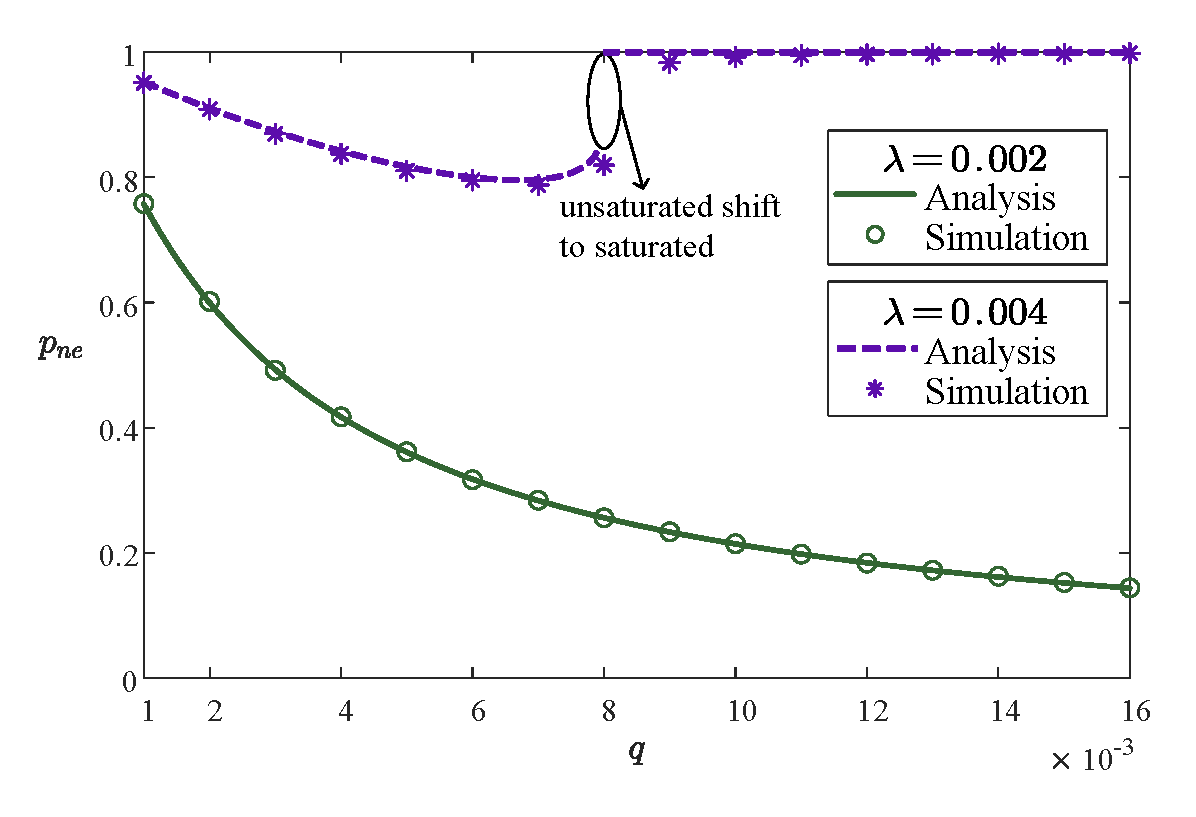
\includegraphics[width=\linewidth]{figure/chap3/p_ne_vs_q.pdf}
		\caption{节点缓存非空概率$p_{ne}$}
		\label{fig:p_ne}
	\end{subfigure}
	\hfill
	\begin{subfigure}{0.485\textwidth}
		\centering
		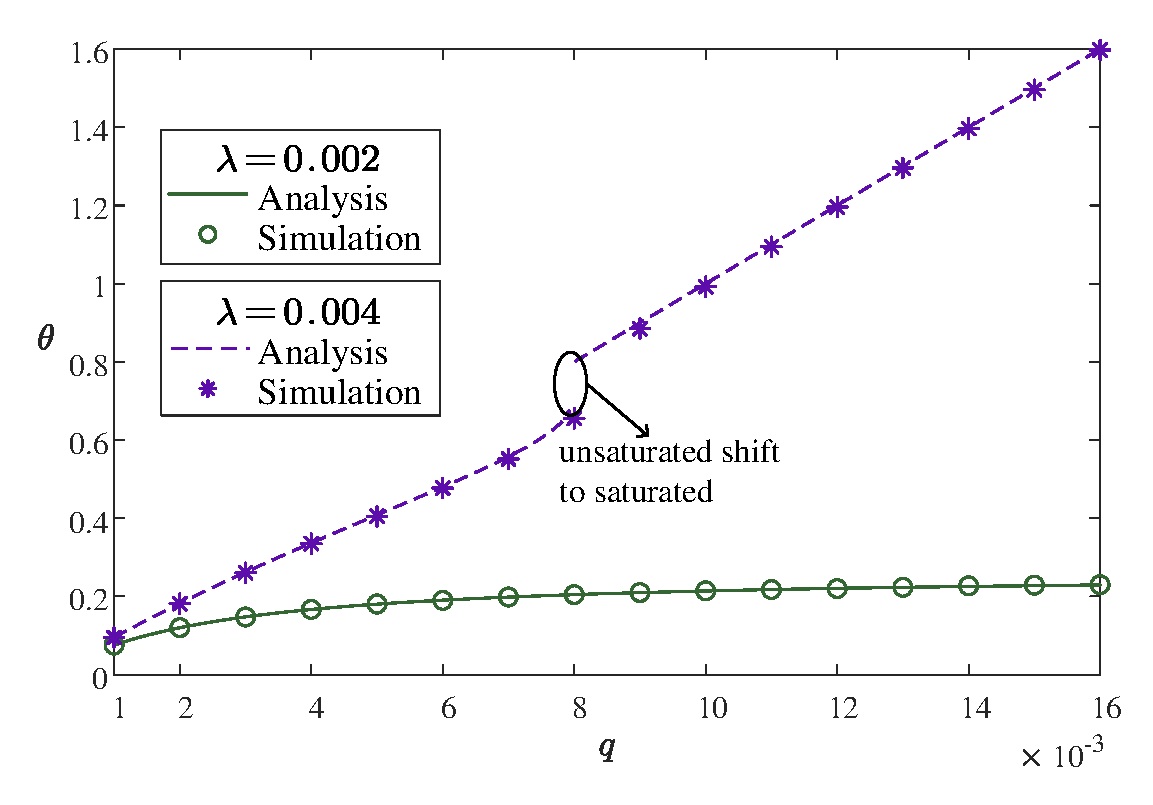
\includegraphics[width=\linewidth]{figure/chap3/theta_vs_q.pdf}
		\caption{尝试速率$\theta$}
		\label{fig:theta}
	\end{subfigure}
	
	\begin{subfigure}{0.495\textwidth}
		\centering
		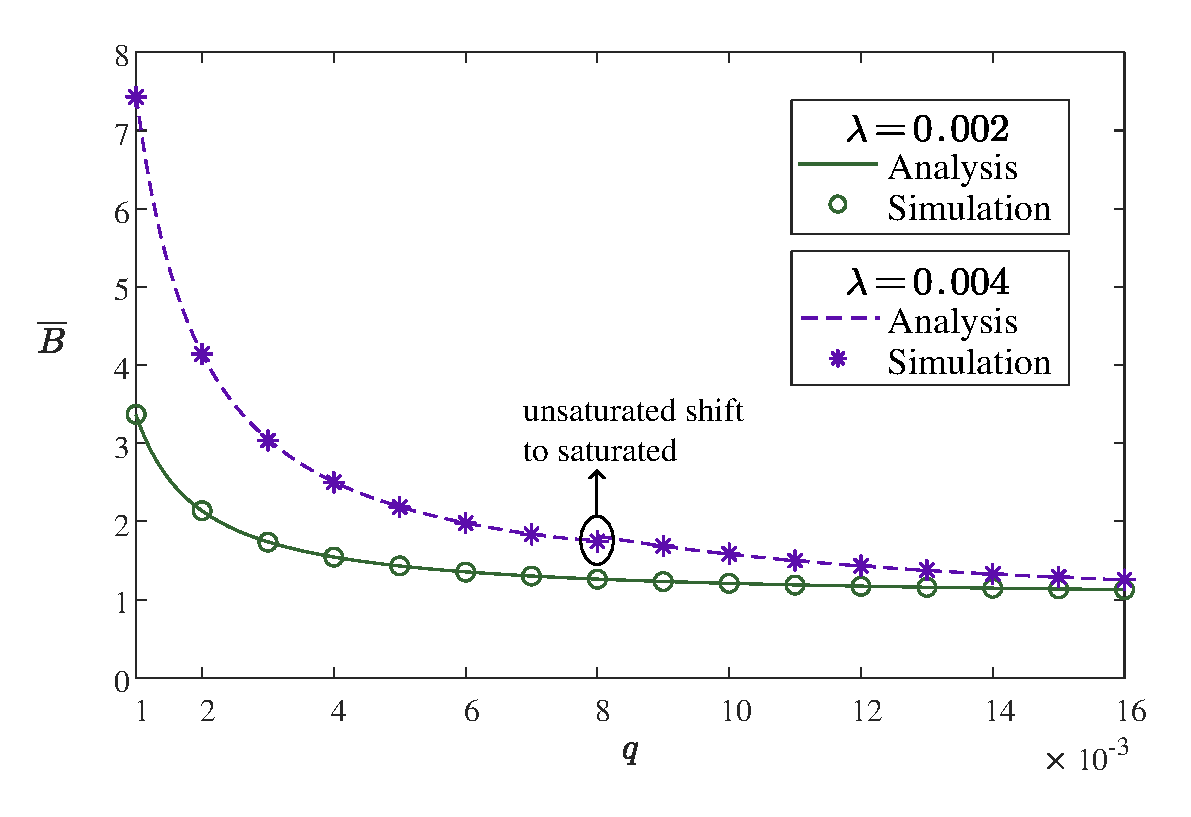
\includegraphics[width=\linewidth]{figure/chap3/mean_B_vs_q.pdf}
		\caption{信道忙期平均长度$\overline{B}$}
		\label{fig:mean_B}
	\end{subfigure}
	\hfill
	\begin{subfigure}{0.485\textwidth}
		\centering
		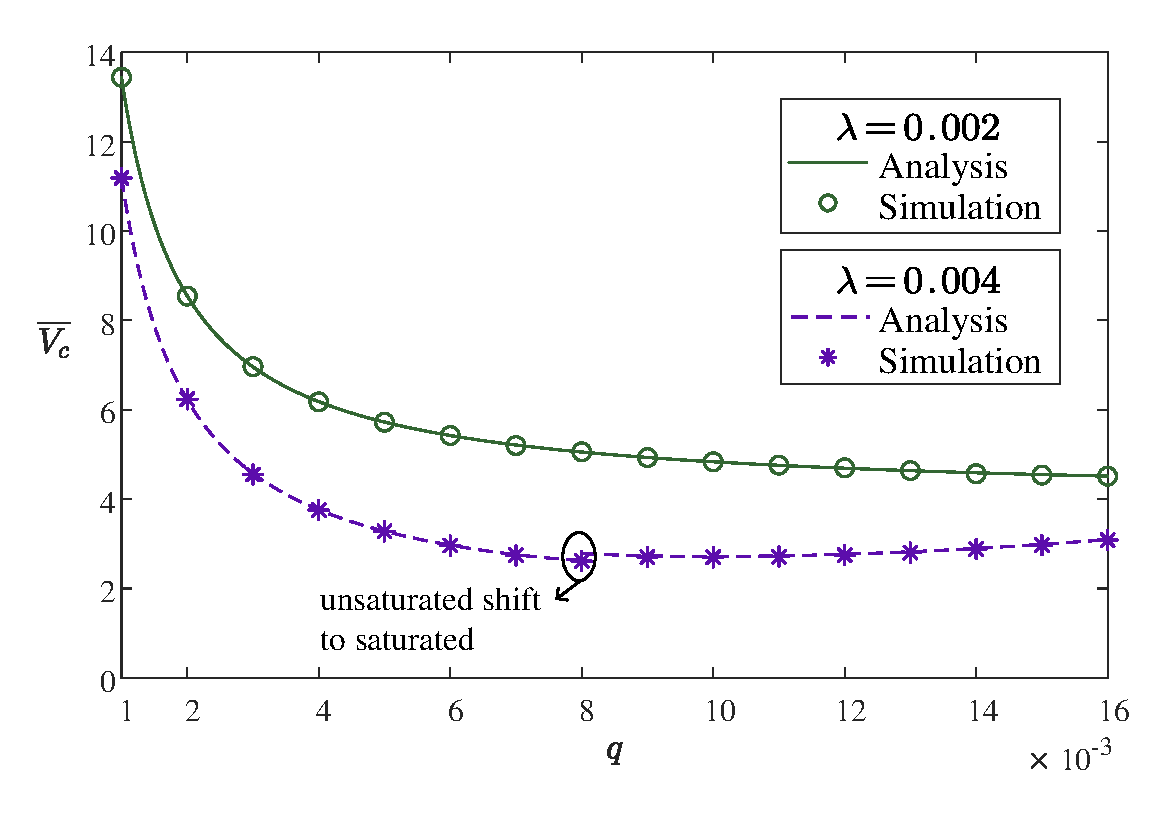
\includegraphics[width=\linewidth]{figure/chap3/mean_Vc_vs_q.pdf}
		\caption{信道假期平均长度$\overline{V}_c$}
		\label{fig:mean_Vc}
	\end{subfigure}
	\caption{系统参数随传输概率$q$的变化情况，$n=100$，$\lambda = \hat{\lambda}/n \in \{0.002, 0.004\}$}
	\label{fig:system_parameters}
\end{figure}

图 \ref{fig:p_ne} 至图 \ref{fig:mean_Vc} 展示了系统关键参数随传输概率 $q$ 的变化趋势。根据节点输入速率的不同，网络表现出两种截然不同的行为模式。首先，在轻负载条件下，例如 $\lambda=0.002$，网络始终处于非饱和稳态。随着传输概率 $q$ 的增加，尝试速率 $\theta$ 随之上升，表明接入竞争更加频繁。然而，由于信道资源尚有富余，较高的发送概率加速了数据包传输，使得节点能够更快地清空缓存。因此，节点缓存非空概率 $p_{ne}$、平均忙期 $\overline{B}$ 以及平均信道假期 $\overline{V}_c$ 均呈现单调递减趋势。
相比之下，在重负载条件下，例如 $\lambda=0.004$，系统行为出现明显差异。如图 \ref{fig:theta} 所示，随着 $q$ 的增加，曲线出现了一个明显转折点，标志着网络从非饱和状态向饱和状态转变。
其原因在于，当 $q$ 过大时，剧烈的信道竞争导致碰撞率飙升，系统的有效吞吐量开始低于数据包的到达速率。这导致数据包在节点缓存中迅速积压，使得节点缓存非空概率 $p_{ne}$ 迅速攀升并锁定在 1，网络随即陷入饱和。
在此饱和区域内，系统的尝试速率不再满足非饱和定点方程（式 \ref{eq:theta_fixed_point}），而是转由饱和条件下的线性关系 $\theta_{sa} = nq$ 主导。此外，图 \ref{fig:mean_B} 和图 \ref{fig:mean_Vc} 分别记录了该相变过程对平均忙期 $\overline{B}$ 和平均假期 $\overline{V}_c$ 的影响。可以观察到，尽管网络状态发生了根本性切换，这两个指标在饱和区的数值变化幅度相对平缓。



\section{吞吐量性能分析}
\label{sec:throughput_analysis}

本节基于前文休假排队模型分析 SAST机制下的吞吐量。为了探究 SAST 机制的性能极限，我们考虑网络处于饱和状态这一场景。在这一场景中，节点缓存始终非空（$p_{ne}=1$）、缓存清空概率为零（$p_0=0$），因此尝试速率为 $\theta_{sa}=nq$。将上述条件代入式 (\ref{eq:mean_vc_derived}) 与 $\overline{B}_{sa}$ 的表达式，可得饱和状态下的平均周期参数分别为	$ \overline{V}_{c,sa} = \frac{e^{nq}}{nq}, \quad \overline{B}_{sa} = \frac{1}{1 - e^{-nq}} $。
在将该结果代入吞吐量定义式，可得吞吐量的表达式为：
\begin{equation}
	\label{eq:access_throughput_sa}
	\lambda_{out}^a = \frac{nq (1 - e^{-nq})}{nq + e^{nq} - 1},
\end{equation}

\begin{equation}
	\label{eq:data_throughput_sa}
	\lambda_{out}^d = \frac{nq}{nq + e^{nq} - 1}.
\end{equation}
基于上述闭式解，我们可以通过调节传输概率 $q$ 来优化系统性能。以下两个定理分别给出了接入吞吐量和数据吞吐量的理论极限。
\begin{theorem}[最大接入吞吐量]
	\label{thm:max_access_throughput}
	当网络处于饱和状态时，SAST 机制的最大接入吞吐量约为 0.2384。该最大值当且仅当传输概率 $q$ 满足特定最优条件时取得：
	\begin{equation}
		\max_{q} \lambda_{out}^a \approx 0.2384, \quad \text{条件：} q^* \approx \frac{1.2515}{n}.
	\end{equation}
\end{theorem}

\begin{proof}
	令 $x = nq$，构造函数 $f(x) = \lambda_{out}^a(x)$。对 $f(x)$ 求导并令 $f'(x) = 0$，可得关于 $x$ 的超越方程。通过数值方法求解该方程，可得极值点位于 $x_0 \approx 1.2515$ 处，对应的函数极大值为 $f(x_0) \approx 0.2384$。
%	详细的导数推导及数值求解过程参见\textbf{附录 D}。
\end{proof}
\begin{theorem}[最大数据吞吐量]
	\label{thm:max_data_throughput}
	当网络处于饱和状态时，数据吞吐量 $\lambda_{out}^d$ 是关于总负载 $nq$ 的单调递减函数。SAST 机制的理论最大数据吞吐量为 0.5，且在传输概率趋近于 0 时取得：
	\begin{equation}
		\lambda_{max}^d = \lim_{nq \to 0} \lambda_{out}^d = \frac{1}{2}.
	\end{equation}
\end{theorem}

\begin{proof}
	令 $x = nq$，构造函数 $g(x) = \lambda_{out}^d(x) = \frac{x}{x + e^x - 1}$。对 $g(x)$ 求导，可证在 $x > 0$ 的区间内 $g'(x) < 0$ 恒成立，即数据吞吐量随负载增加而单调递减。
	为了求取最大值，利用洛必达法则对 $x \to 0$ 处求极限：
	\[
	\lim_{x \to 0} \frac{x}{x + e^x - 1} = \lim_{x \to 0} \frac{1}{1 + e^x} = \frac{1}{2}.
	\]
%	详细的单调性证明过程参见\textbf{附录 D}。
\end{proof}
%定理 \ref{thm:max_data_throughput} 揭示了 SAST 机制的核心优势：通过降低传输概率 $q$（即 $nq \to 0$），虽然成功接入的频次降低，但单次接入后的平均忙期长度 $\overline{B}_{sa}$ 显著增加，从而能够极其高效地填充信道，突破了传统 Aloha 协议 $e^{-1} \approx 0.368$ 的性能瓶颈。
\begin{figure}[t]
	\centering
	% --- 子图 (a): 接入吞吐量 ---
	\begin{subfigure}[b]{0.495\textwidth}
		\centering
		% 请替换为您实际的图片文件名
		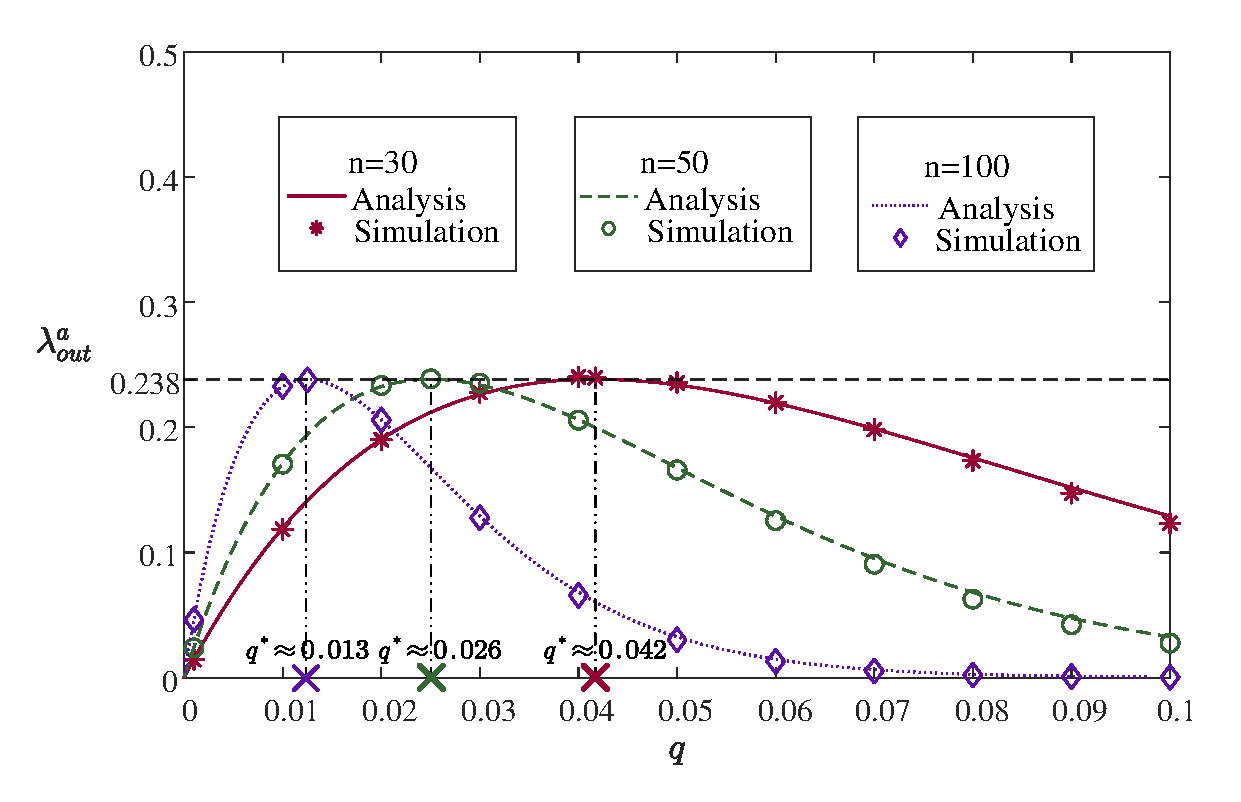
\includegraphics[width=\textwidth]{figure/chap3/access_throughput_vs_q.pdf}
		\caption{接入吞吐量 $\lambda_{out}^a$}
		\label{fig:sub_access}
	\end{subfigure}
	\hfill % 在两个子图之间添加弹性间距
	% --- 子图 (b): 数据吞吐量 ---
	\begin{subfigure}[b]{0.495\textwidth}
		\centering
		% 请替换为您实际的图片文件名
		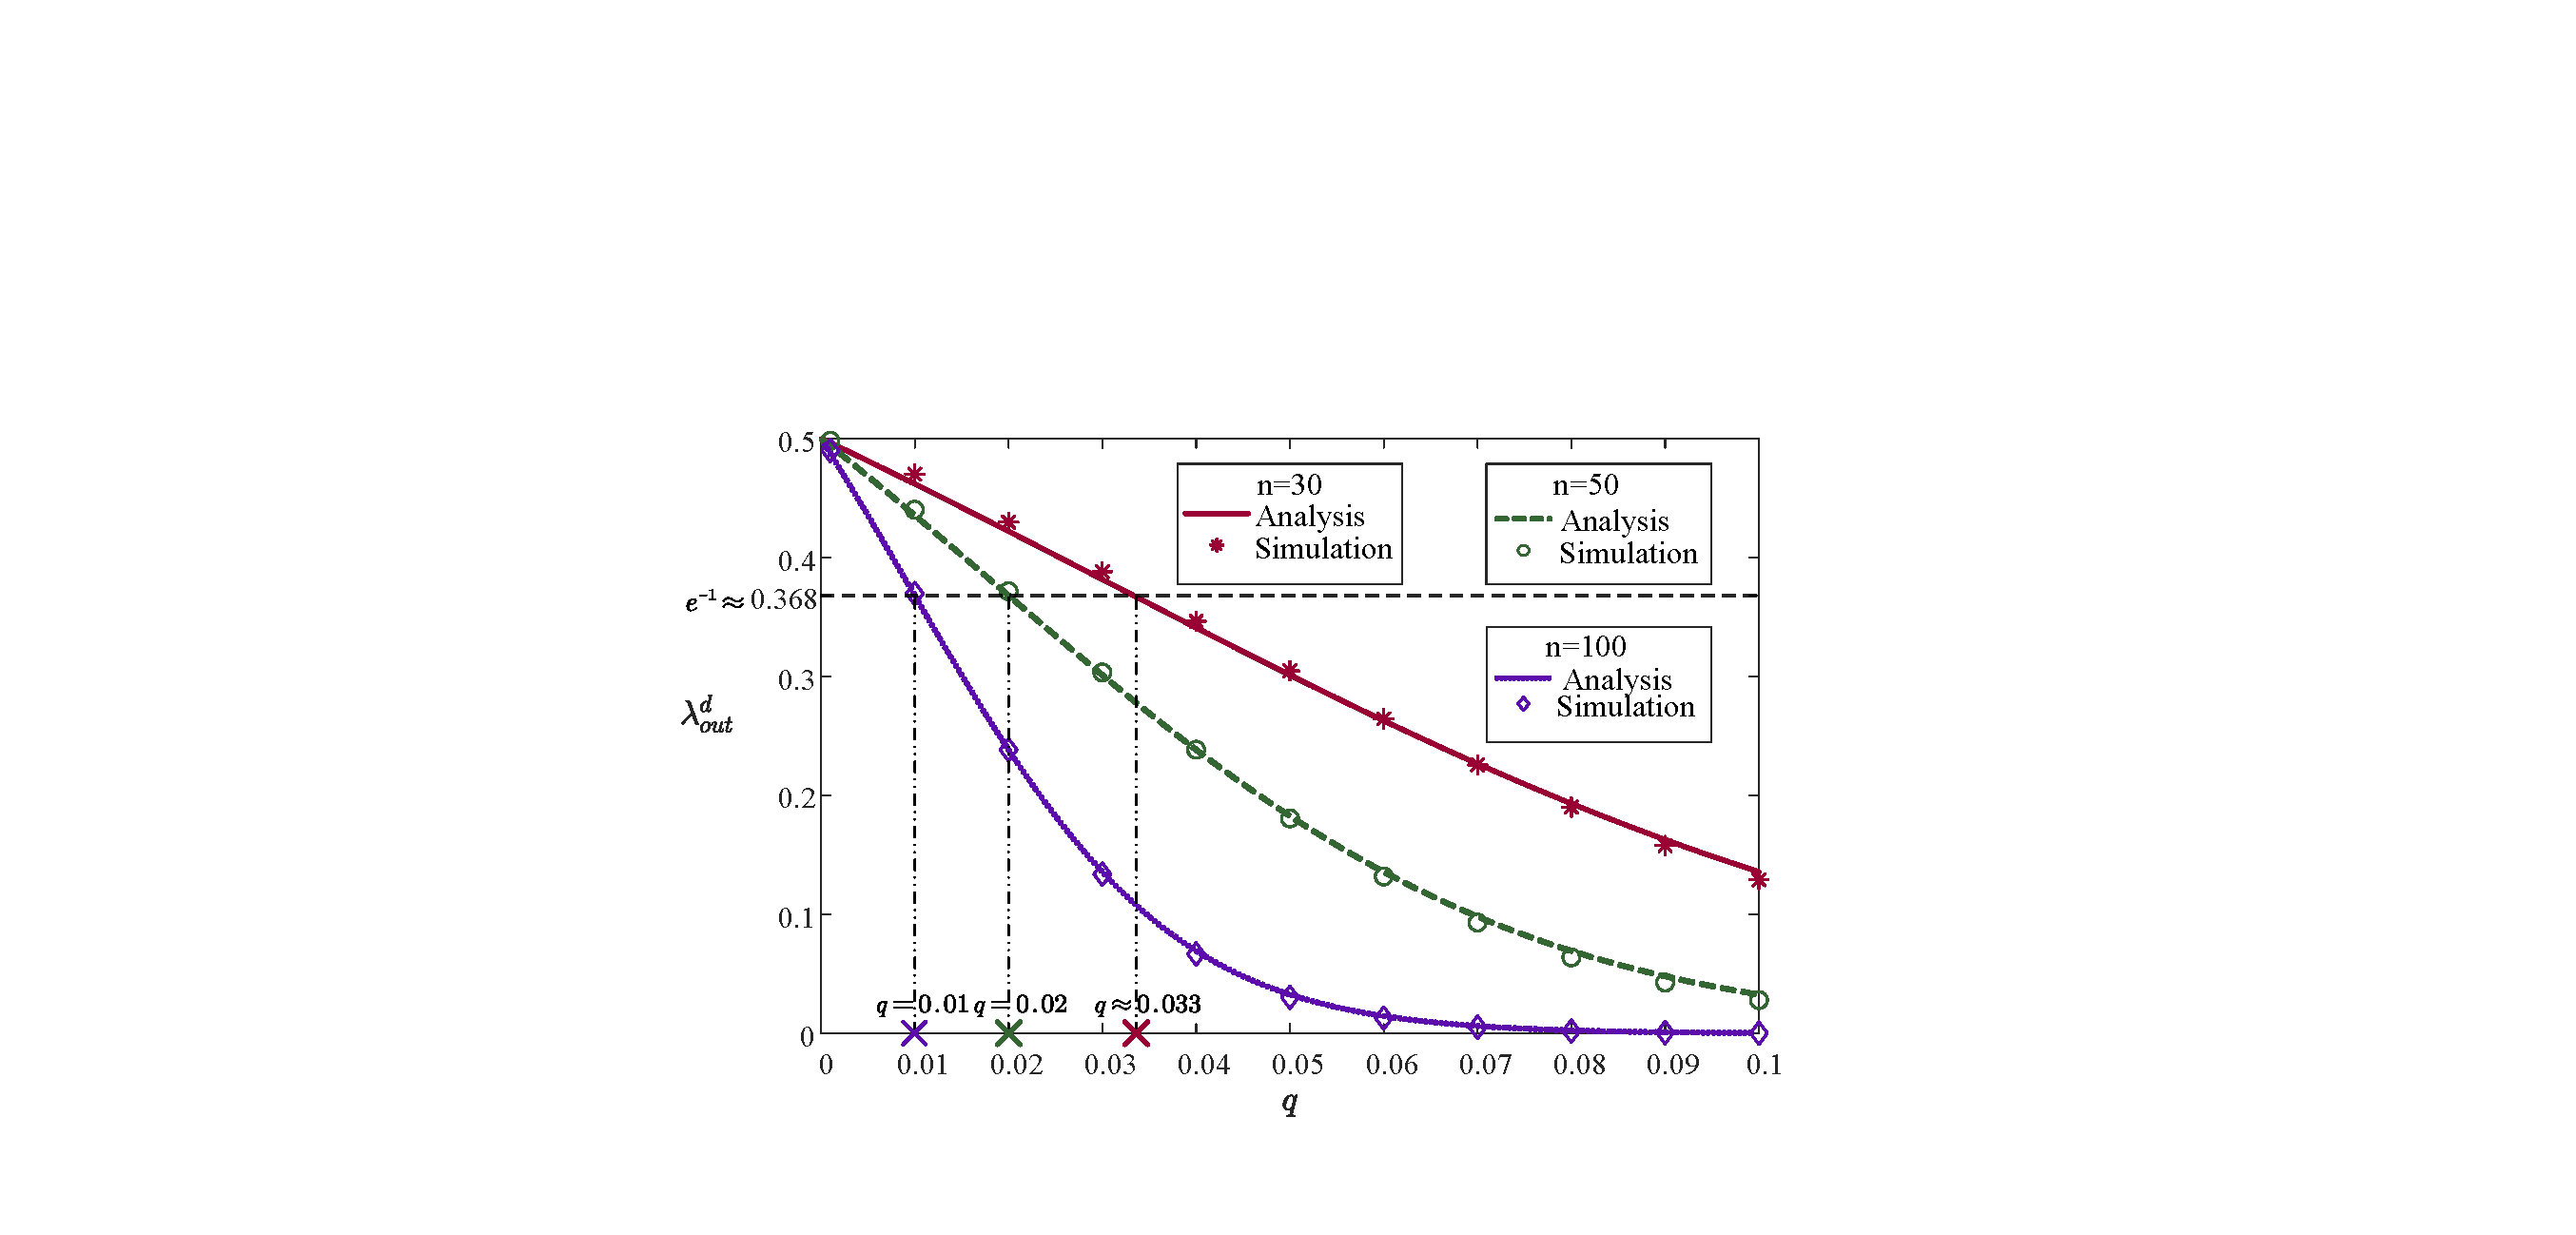
\includegraphics[width=\textwidth]{figure/chap3/data_throughput_vs_q.pdf}
		\caption{数据吞吐量 $\lambda_{out}^d$}
		\label{fig:sub_data}
	\end{subfigure}
	
	\caption{饱和状态下的吞吐量性能随传输概率 $q$ 的变化，$n \in \{30, 50, 100\}$}
	\label{fig:throughput_vs_q}
\end{figure}


为了验证上述理论推导的准确性，图 \ref{fig:throughput_vs_q} 展示了在饱和状态下，接入吞吐量 $\lambda_{out}^a$ 和数据吞吐量 $\lambda_{out}^d$ 随传输概率 $q$ 的变化情况。仿真中设置节点数量 $n \in \{30, 50, 100\}$。
如图~\ref{fig:sub_access} 所示，接入吞吐量随接入概率 $q$ 呈现出典型的先增后减的凸函数特征。在较小的 $q$ 区域内，节点发起接入的概率较低，系统整体处于轻载状态，此时信道竞争较弱，多数时隙处于空闲或仅有少量节点参与竞争的状态，虽然单次接入成功概率较高，但由于单位时间内的接入尝试次数有限，成功接入事件的总体数量受到限制，从而使接入吞吐量维持在较低水平。随着 $q$ 的逐步增大，参与竞争的节点数量增加，系统中的接入尝试频率提升，在碰撞尚未成为主导因素之前，成功接入事件的发生频率随之增加，从而推动接入吞吐量不断上升。当 $q$ 进一步接近最优点 $q^*$ 时，系统达到接入尝试频率与碰撞概率之间的平衡状态，此时单位时隙内平均参与竞争的节点数量处于一个最优水平，使得接入吞吐量达到峰值。随着 $q$ 超过该临界值，系统逐渐进入高竞争区域，大量节点在同一时隙内同时发起接入请求，导致碰撞概率迅速上升，而随机接入成功要求恰有一个节点发送，因此多节点同时发送会使成功概率呈指数形式下降，尽管接入尝试频率仍在增加，但绝大多数尝试由于碰撞而失效，信道被大量无效竞争占用，最终导致接入吞吐量快速下降。此外也可以观察到，其最优接入概率 $q^*$ 也不是 $\frac{1}{n}$，而是 $\frac{1.2515}{n}$；其根本原因在于连续传输机制导致最优点发生了偏移。



另一方面，图~\ref{fig:sub_data} 展示了数据吞吐量随接入概率 $q$ 的变化规律。可以观察到，随着 $q$ 的增大，数据吞吐量整体呈现单调递减趋势。以经典时隙 Aloha 的最大吞吐量 $e^{-1} \approx 0.368$ 作为基准线，当系统总负载满足 $nq < 1$ 时，SAST 机制的数据吞吐量始终高于该基准，并可接近 0.5。这一现象源于接入频率与碰撞概率之间的权衡关系，即较小的 $q$ 虽然降低了节点发起接入的频率，但同时抑制了多节点同时发送所引发的碰撞概率，从而使节点一旦成功接入信道，能够维持较长的连续传输过程，使平均忙期长度 $\overline{B}$ 增加，并通过更长时间的信道占用来承载更多数据传输。
随着 $q$ 的增大，系统竞争强度逐渐增强，碰撞概率上升，不仅降低了接入成功概率，更会频繁打断已经建立的连续传输过程，从而导致忙期长度缩短。尽管更大的 $q$ 在一定程度上有利于增加成功接入事件的发生次数，但由于连续传输阶段被频繁打断，使单次成功接入所能传输的数据包数量减少，且这种下降速度快于接入频率提升所带来的收益增长，因此系统整体吞吐量呈现出持续下降的趋势。
特别地，这一单调下降特性与经典时隙 Aloha 中的凸性规律本质不同，其根本原因在于系统吞吐量的主导因素发生了转变。系统性能主要由单位时隙内的成功接入概率决定，因此在较小的 $q$ 区域内，随着节点发送概率的提高，成功发送事件的发生频率增加，从而带来吞吐量的提升；而当 $q$ 进一步增大时，多用户竞争导致的碰撞概率迅速上升并逐渐占据主导地位，最终使吞吐量下降，形成典型的凸形变化趋势。然而在 SAST 机制中，数据吞吐量不仅取决于接入成功的发生频率，还与单次成功接入后所能维持的连续传输时长，即忙期长度$\overline{B}$ 密切相关，系统整体性能可以理解为接入成功过程与连续占用信道过程的共同结果。



\section{时延性能分析}
\label{sec:delay_analysis}
除了吞吐量之外，时延是衡量随机接入机制性能的另一项关键指标。本节将分别对接入时延 $D_A$ 和数据包时延 $D_P$ 进行推导。

\subsection{接入时延 $D_A$ 推导与分析}

接入时延 $D_A$ 定义为节点生成的队首数据包从进入队首开始，到成功被基站接收并收到确认反馈为止所经历的平均时长。
从前文节点休假模型可知，接入过程本质上对应于类型 1 假期，即节点在缓存非空的情况下不断竞争信道直至成功的时段。因此，接入时延在数值上等同于类型 1 假期的平均长度：
\begin{equation}
	D_A = \overline{V}_1.
\end{equation}

结合前文关于类型 1 假期的新包到达过程 $A_{V_1}$ 的推导以及节点输入的伯努利特性，根据排队论中的 Little 定律，可得 $D_A = \overline{V}_1 = \frac{\overline{A}_{V_1}}{\lambda}$。
将前文推导的 $\overline{A}_{V_1}$ 闭式解代入，可得非饱和情况下，接入时延的通用表达式：
\begin{equation}
	\label{eq:access_delay_general}
	D_A = \frac{\theta}{n q \lambda \left(1 - \frac{\theta}{n q} e^{-\theta}\right)}.
\end{equation}

特别地，当网络处于饱和状态时，我们从单节点的接入吞吐量与其平均接入时延之间的关系出发。注意，此时节点的所有假期都为类型1假期。
单节点的接入吞吐量可以表示为 $\lambda_{out}^a / n = \frac{1}{\overline{ B }+ \overline{V_{1,sa}}}= \frac{q(1 - e^{-nq})}{nq+e^{nq}-1}$。由此可得饱和状态下的平均接入时延为
\begin{equation}
	\label{eq:access_delay_sa}
	D_{A,sa} = \overline{V}_{1,sa} = \frac{e^{nq} + nq - 1 - q}{q(1 - e^{-nq})}.
\end{equation}
该式表明，在饱和状态下，接入时延主要受总负载 $nq$ 的指数增长项主导。


\subsection{数据包时延 $D_P$ 推导与分析}
数据包时延 $D_P$ 定义为数据包从生成时刻起到成功传输完毕离开系统所需的平均时长，该指标由排队等待时间和传输服务时间两部分组成。
需要说明的是，数据包时延的稳态分析仅在网络处于非饱和状态，即数据吞吐量等于输入速率 $\lambda_{out}^d = n\lambda$ 时有效。若网络处于饱和状态，节点缓存队列长度发散，导致理论上的平均包时延趋于无穷大。

为了求解 $D_P$，我们借助排队论中的 Little 定律 $D_P = \frac{\overline{L}}{\lambda}$，其中 $\overline{L}$ 为节点缓存队列的平均长度。因此，问题的核心转化为求解稳态下的平均队长 $\overline{L}$。
为此，我们引入一个二维马尔可夫链 $(L_t, K_t)$ 来刻画节点队列的动态行为，如图 \ref{fig:markov_chain} 所示。其中，$L_t \in \{0, 1, \dots\}$ 表示时隙 $t$ 开始时的队列长度，$K_t \in \{0, 1\}$ 为状态指示变量，$K_t=1$ 表示节点处于忙期，$K_t=0$ 表示节点处于假期。

\begin{figure}[t]
	\centering
	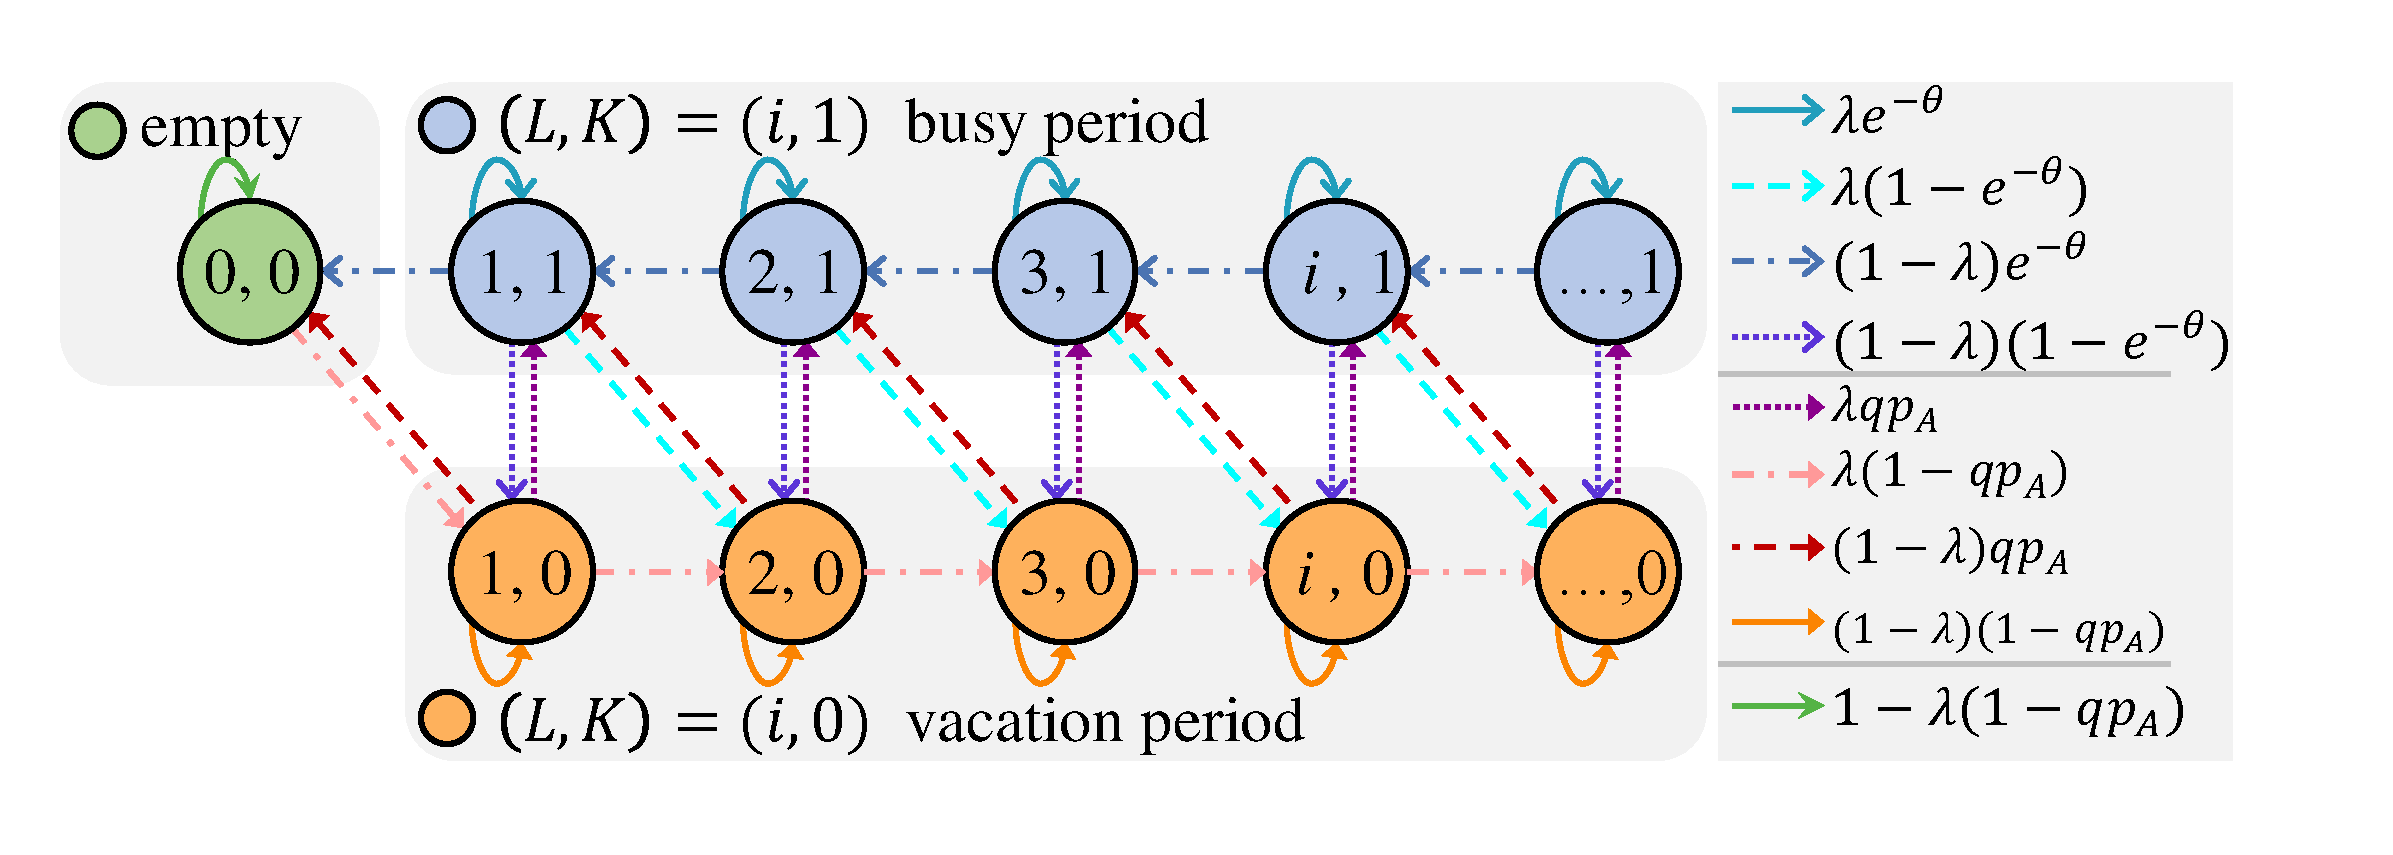
\includegraphics[width=0.95\textwidth]{figure/chap3/2Dmarkov_chain.pdf}
	\caption{节点队列长度在时隙 $t$ 的状态转移马尔可夫链 $(L_t, K_t)$}
	\label{fig:markov_chain}
\end{figure}
通过求解该马尔可夫链的平衡方程，可得其稳态概率分布 $\pi_{i,k} = \lim_{t\to\infty} \Pr\{L_t=i, K_t=k\}$ 如下：
\begin{equation}
	\label{eq:steady_state_prob}
	\begin{cases}
		\pi_{10} = \left( \dfrac{1}{1 - \frac{\lambda}{1-\lambda}\gamma} + \dfrac{\lambda}{1-\lambda} - 1 + \dfrac{1}{1-\gamma} + \dfrac{(1-\lambda)p_A + \lambda e^{-\theta}}{\lambda(1-p_A)} \right)^{-1} \\
		\pi_{00} = \dfrac{(1-\lambda)p_A + \lambda e^{-\theta}}{\lambda(1-p_A)} \pi_{10} \\
		\pi_{11} = \dfrac{\lambda}{1-\lambda} \pi_{10} \\
		\pi_{i0} = \gamma^{i-1} \pi_{10}, \quad i \geq 2 \\
		\pi_{i1} = \dfrac{\lambda}{1-\lambda} \pi_{i0} = \left( \dfrac{\lambda}{1-\lambda} \gamma \right)^{i-1} \pi_{10}, \quad i \geq 2
	\end{cases}
\end{equation}
式中，参数 $\gamma$ 定义为
$ 	\gamma = \frac{\lambda[\lambda(1-e^{-\theta}) + (1-\lambda)(1-p_A)]}{(1-\lambda)(\lambda e^{-\theta} + (1-\lambda)p_A)}$。 $p_A$ 定义为接入请求概率。
基于稳态分布，节点缓存队列的平均长度可由期望公式计算得出：$\overline{L} = \mathbb{E}[\pi] = \sum_{i=1}^{\infty} (\pi_{i0} + \pi_{i1}) i$。

在 SAST 机制中，队首数据包成功接入的前提是信道处于可用状态且其余节点未同时竞争。信道可用包含两种互斥情况：一是信道处于休假状态，其概率为 $1 - \lambda_{out}^{d}$；二是信道处于忙期的最后一个时隙，且当前传输节点在该忙期结束时恰好清空缓存。后一事件在每个信道周期中至多出现一次，因此对应概率可写为 $p_0 / \overline{C}_c$。进一步结合其余 $n-1$ 个节点的静默概率 $e^{-\theta}$，可得接入成功概率 $p_A$ 为：
\begin{equation}
	\label{eq:pA_expression}
	p_A = \left(1 - \frac{\lambda \theta}{q}\right) e^{-\theta}
\end{equation}
将 $p_A$ 代入稳态分布并求和，得到节点缓存队列平均长度 $\overline{L}$ 的闭式解：
\begin{equation}
	\label{eq:mean_queue_length}
	\overline{L} = \frac{ \frac{1}{1-\lambda} + \frac{\gamma(2-\gamma)}{(1-\gamma)^2} + \frac{\frac{\lambda\gamma}{1-\lambda} \left(2 - \frac{\lambda\gamma}{1-\lambda}\right)}{\left(1 - \frac{\lambda\gamma}{1-\lambda}\right)^2} }{ \frac{1}{1 - \frac{\lambda\gamma}{1-\lambda}} + \frac{\lambda}{1-\lambda} - 1 + \frac{1}{1-\lambda} + \frac{(1-\lambda)p_A + \lambda e^{-\theta}}{\lambda(1-p_A)} }.
\end{equation}
最终，将式 \eqref{eq:mean_queue_length} 除以输入速率 $\lambda$，即可得到非饱和状态下的平均数据包时延 $D_P$：
\begin{equation}
	\label{eq:mean_packet_delay}
	D_P = \frac{ \frac{1}{1-\lambda} + \frac{\gamma(2-\gamma)}{(1-\gamma)^2} + \frac{\frac{\lambda\gamma}{1-\lambda} \left(2 - \frac{\lambda\gamma}{1-\lambda}\right)}{\left(1 - \frac{\lambda\gamma}{1-\lambda}\right)^2} }
	{ \lambda ( \frac{1}{1 - \frac{\lambda\gamma}{1-\lambda}} + \frac{\lambda}{1-\lambda} - 1 + \frac{1}{1-\lambda} + \frac{(1-\lambda)p_A + \lambda e^{-\theta}}{\lambda(1-p_A)} )} .
\end{equation}
尽管式 \eqref{eq:mean_packet_delay} 形式较为复杂，但它建立了时延与系统参数（$n, q, \lambda$）之间的准确关系，为后续的时延性能优化提供了理论依据。
\begin{figure}[t]
	\centering
	\begin{subfigure}{0.495\textwidth}
		\centering
		% 请确保路径和文件名正确
		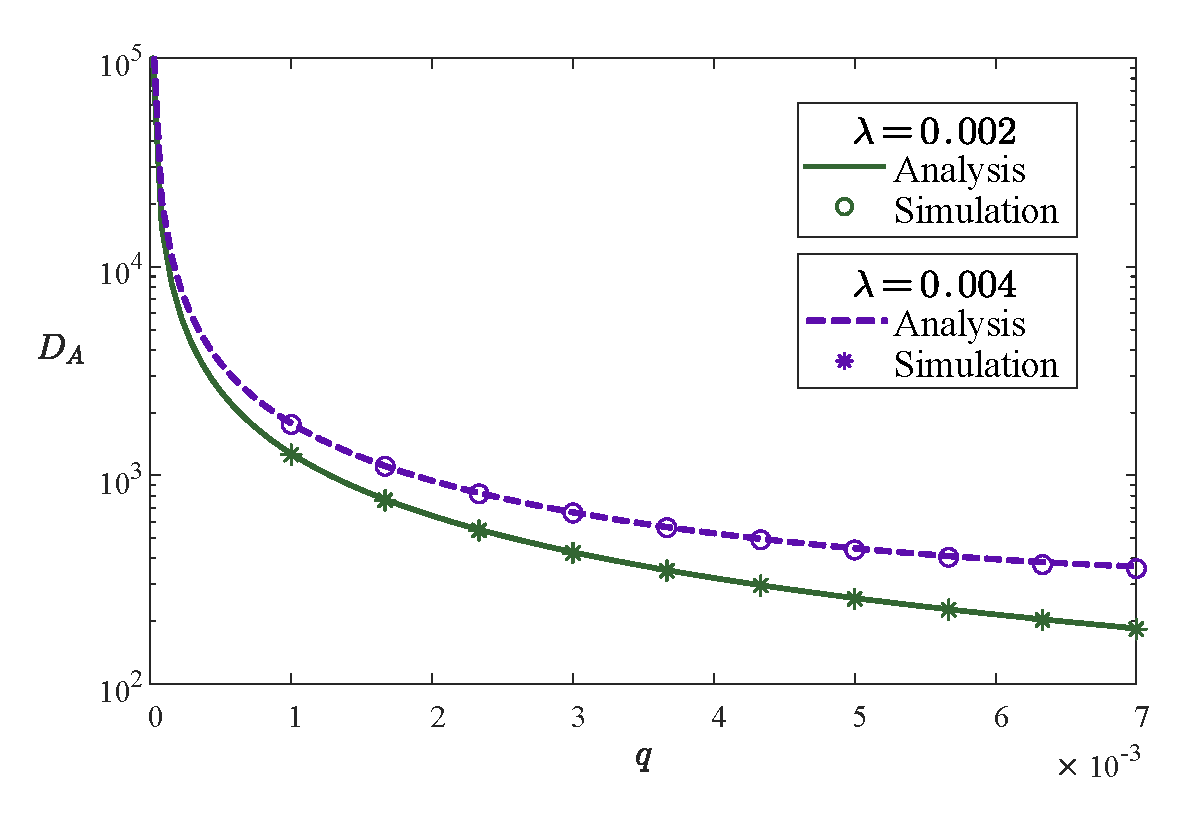
\includegraphics[width=\linewidth]{figure/chap3/access_delay_unsaturated.pdf}
		\caption{非饱和情况下平均接入时延 $D_A$}
		\label{fig:access_delay_unsaturated}
	\end{subfigure}
	\hfill
	\begin{subfigure}{0.495\textwidth}
		\centering
		% 请确保路径和文件名正确
		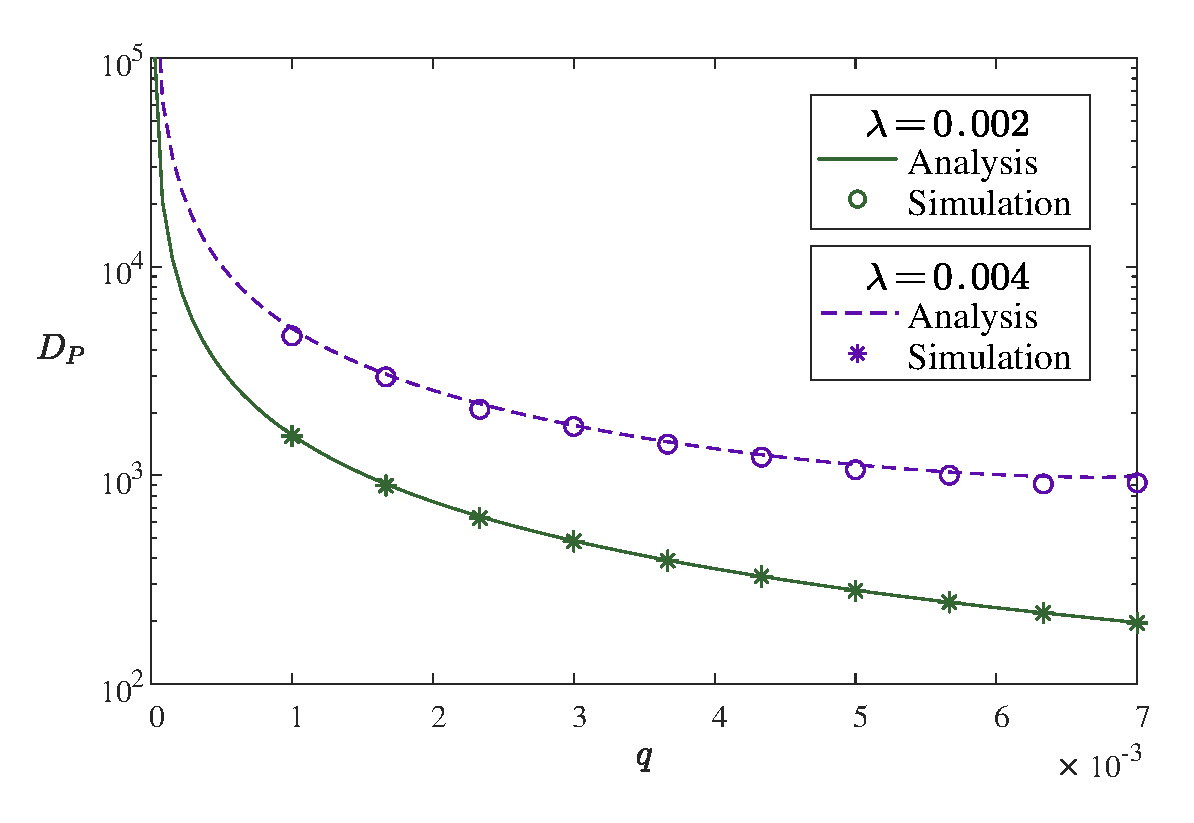
\includegraphics[width=\linewidth]{figure/chap3/packet_delay_unsaturated.pdf}
		\caption{非饱和情况下平均数据包时延 $D_P$}
		\label{fig:packet_delay_unsaturated}
	\end{subfigure}
	
	\begin{subfigure}{0.495\textwidth}
		\centering
		% 请确保路径和文件名正确
		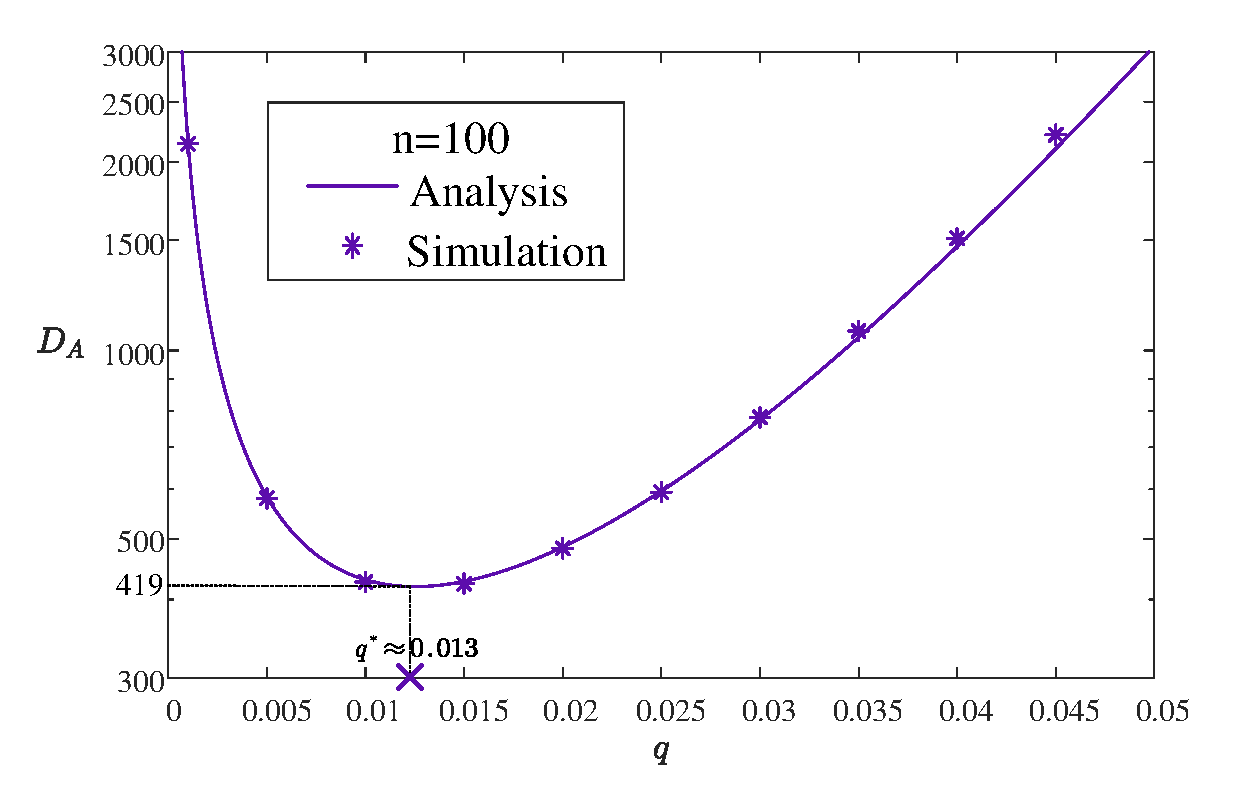
\includegraphics[width=\linewidth]{figure/chap3/access_delay_saturated.pdf}
		\caption{饱和情况下平均接入时延 $D_{A,sa}$}
		\label{fig:access_delay_saturated}
	\end{subfigure}
	\caption{时延随传输概率$q$的变化情况，$n=100$，$\lambda = \hat{\lambda}/n \in \{0.002, 0.004\}$}
	\label{fig:delay_vs_q}
\end{figure}


为了展示 SAST 机制的时延特性，图 \ref{fig:delay_vs_q} 给出了接入时延和数据包时延随传输概率 $q$ 的变化曲线。
如图 \ref{fig:access_delay_unsaturated} 和图 \ref{fig:packet_delay_unsaturated} 所示，当网络处于非饱和状态时，平均接入时延 $D_A$ 和平均包时延 $D_P$ 均随着传输概率 $q$ 的增加而单调递减。
这一现象的原因在于，在轻载（$\lambda=0.002$）或中载（$\lambda=0.004$）条件下，信道资源相对充裕，碰撞并非主要瓶颈。此时，增加 $q$ 使得节点在有数据包到达时能够更积极地尝试接入信道，从而减少了在队列头部的空闲等待时间，实现了数据包的快速发送。
图 \ref{fig:access_delay_saturated} 展示了饱和状态下接入时延 $D_{A,sa}$ 的变化趋势。与非饱和状态截然不同，$D_{A,sa}$ 随 $q$ 呈现出先减后增的凹函数特性。当 $q$ 较小时，增加传输概率有助于利用空闲信道，从而降低时延；当 $q$ 超过一定阈值，对应于最优负载点 $q^*$ 后，信道内的碰撞加剧。此时，节点频繁遭遇传输失败并退避，导致队首数据包滞留时间急剧增加。
对比前文的吞吐量分析可知，饱和接入时延取得最小值的点，恰好对应于接入吞吐量 $\lambda_{out}^a$ 取得最大值的点。这表明在饱和网络中，通过优化 $q$ 可以同时实现接入效率的最优和接入时延的最小化。


\section{SAST 机制在5G小数据传输中的性能评估}
\label{sec:5g_case_study}

\begin{figure}[t]
	\centering
	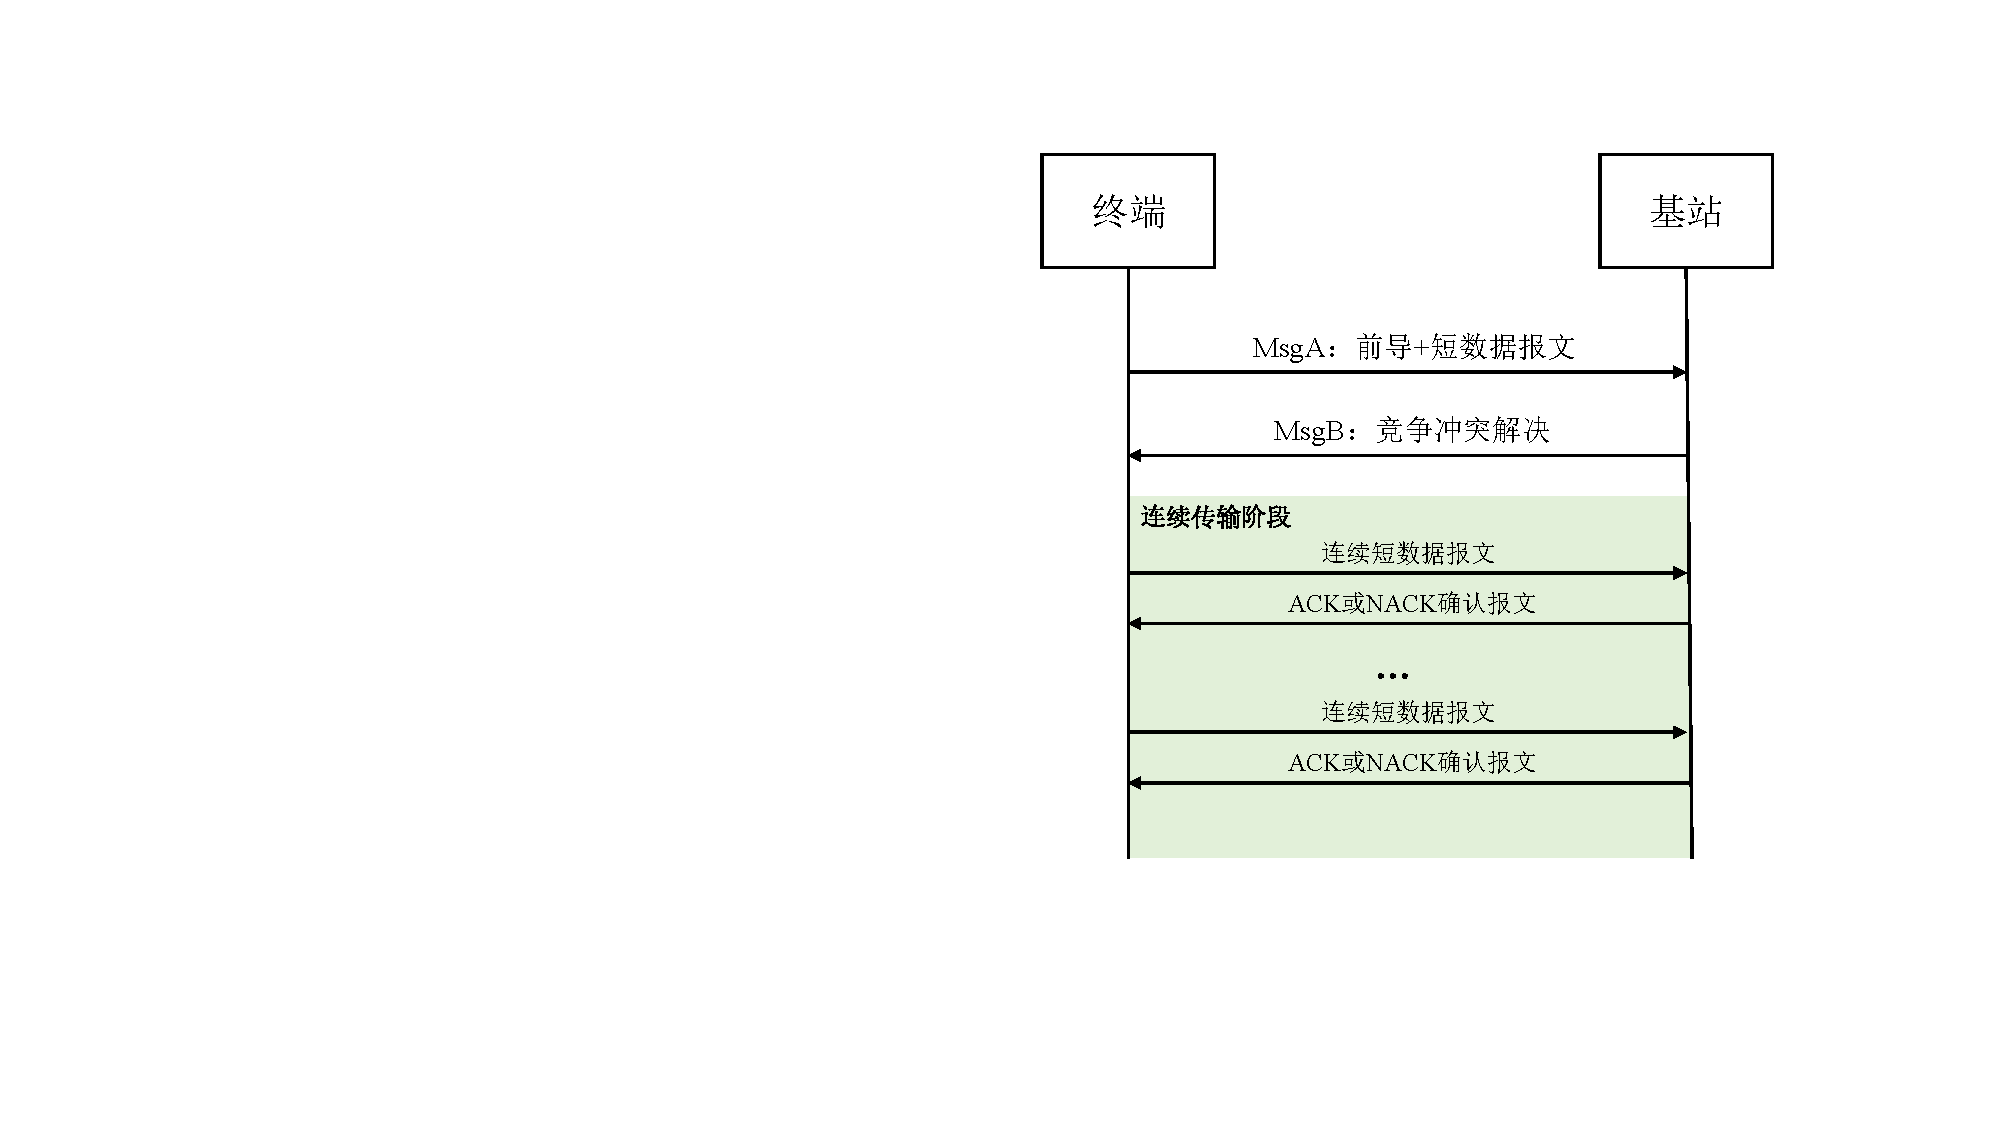
\includegraphics[width=0.65\textwidth]{figure/chap3/sast_scheme.pdf}
	\caption{SAST 方案下，用户与基站间的信令交互流程}
	\label{fig:signaling_process}
\end{figure}

	为了验证 SAST 机制在实际通信系统中的应用潜力，本节将其与 3GPP Release 17 标准中定义的 2 步小数据传输方案作为基准进行对比。为量化两者在控制信令开销方面的差异，本文引入信令吞吐比 $\mathrm{STR}$ 作为核心评估指标。

	\subsection{2 步小数据传输方案}

为克服传统蜂窝网络中 RRC 连接建立过程对小数据包传输造成的效率瓶颈，3GPP R17 标准引入了 2 步小数据传输方案。如图 \ref{fig:sdt_access} 中的 2 步小数据传输过程所示，该方案的核心机制是将物理随机接入信道前导码与上行共享信道的数据载荷合并封装于 MsgA 中发送。基站接收后回复包含竞争解决标识的 MsgB，以确认传输成功；若发生碰撞或解码失败，终端则需退避并重新发起 MsgA 传输。

从信令开销角度看，无论单次接入尝试是否成功，系统物理层都需要承担 MsgA 与 MsgB 两次信令交互的开销。设每次信令交互的平均大小为 $s$ 比特，若系统平均接入成功概率为 $p_A$，则成功传输一个数据包在统计上平均需要 $1/p_A$ 次尝试。据此，2 步小数据传输方案的信令吞吐比可表示为：
\begin{equation}
	\mathrm{STR}_{\mathrm{SDT}} = \frac{2s}{p_A}.
\end{equation}
其中，$p_A$ 可由文献\cite{2012_DaiAloha} 计算得到。这一指标直观地反映了在低接入成功率场景下，标准方案面临的信令效率急剧下降问题。

\subsection{SAST 机制在 5G 中的实现与信令分析}

SAST 机制在 5G 系统中的部署具有较强兼容性，可以复用 3GPP R17 的 2 步小数据传输流程完成初始接入，并在此基础上扩展连续传输能力以提升信令效率。
如图~\ref{fig:signaling_process} 所示，具体流程如下：节点首先将队首数据包封装在包含前导码的 MsgA 中发送，这与标准 2 步小数据传输过程一致。一旦收到基站反馈的 MsgB 并确认接入成功，节点随即进入连续传输阶段。与标准方案不同的是，后续数据包可直接在 PUSCH 信道发送，而无需再次携带前导码。基站对每个后续数据包逐一反馈确认消息；若成功传输一个报文，基站会回馈确认消息；若发生碰撞并收到否定确认消息，节点退回竞争状态。若节点缓存队列清空，则可通过最后一个数据报文中的结束标记告知基站传输即将结束，至此本轮传输自然结束。



为了量化上述机制带来的信令增益，下面分析其信令吞吐比 $\mathrm{STR}$。在 SAST 的一个成功接入周期内，平均可连续传输 $\overline{B}$ 个数据包。除队首数据包外，后续 $\overline{B}-1$ 个数据包的信令开销取决于忙期的结束方式：若传输因缓存清空而正常结束，概率为 $p_0$，则仅消耗对应的确认消息开销；若因碰撞而异常中断，概率为 $1-p_0$，则最后一个失败数据包还会额外消耗一次发送与一次否定确认的信令资源。
综合考虑队首数据包的初始接入与后续传输开销，SAST 的信令吞吐比可推导为：
\begin{equation}
	\mathrm{STR}_{\mathrm{SAST}} = s + \frac{s}{\overline{B}} \left( \frac{2}{p_A} + 1 - 2p_0 \right).
\end{equation}
特别地，在网络处于饱和极限状态下（此时 $p_0=0$ 且 $\theta=nq$），该指标可进一步简化为：
\begin{equation}
	\mathrm{STR}_{\mathrm{SAST}, sa} = s (2e^{nq} + 2nq - e^{-nq}).
\end{equation}
该式表明，在饱和状态下，SAST 通过一次前导码开销换取了多次数据传输机会，从而在理论上降低了单位数据的信令成本。

\subsection{信令开销性能对比}

\begin{figure}[t]
	\centering
	\begin{subfigure}[b]{0.48\textwidth}
		\centering
		% 对应 TCOM Fig. 8a
		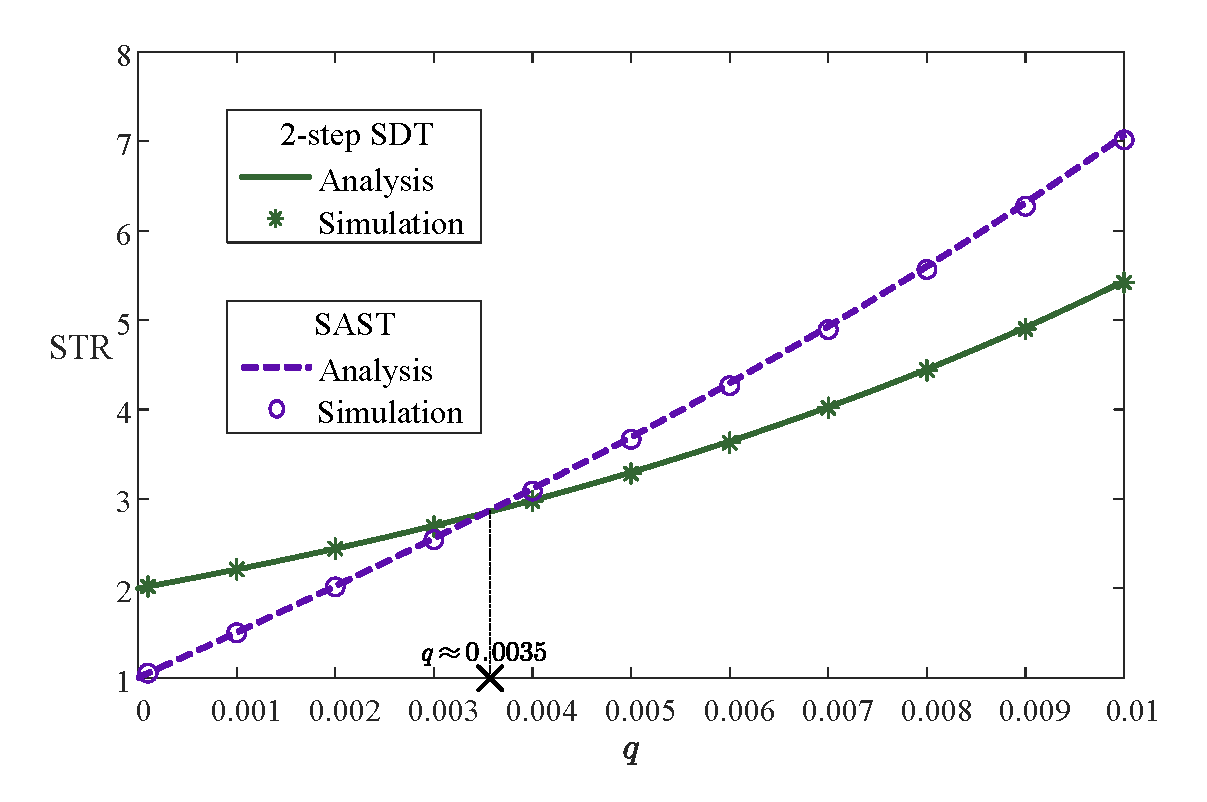
\includegraphics[width=\textwidth]{figure/chap3/str_vs_q_saturated.pdf}
		\caption{饱和状态下的 STR 对比}
		\label{fig:str_sat}
	\end{subfigure}
	\hfill
	\begin{subfigure}[b]{0.49\textwidth}
		\centering
		% 对应 TCOM Fig. 8b
		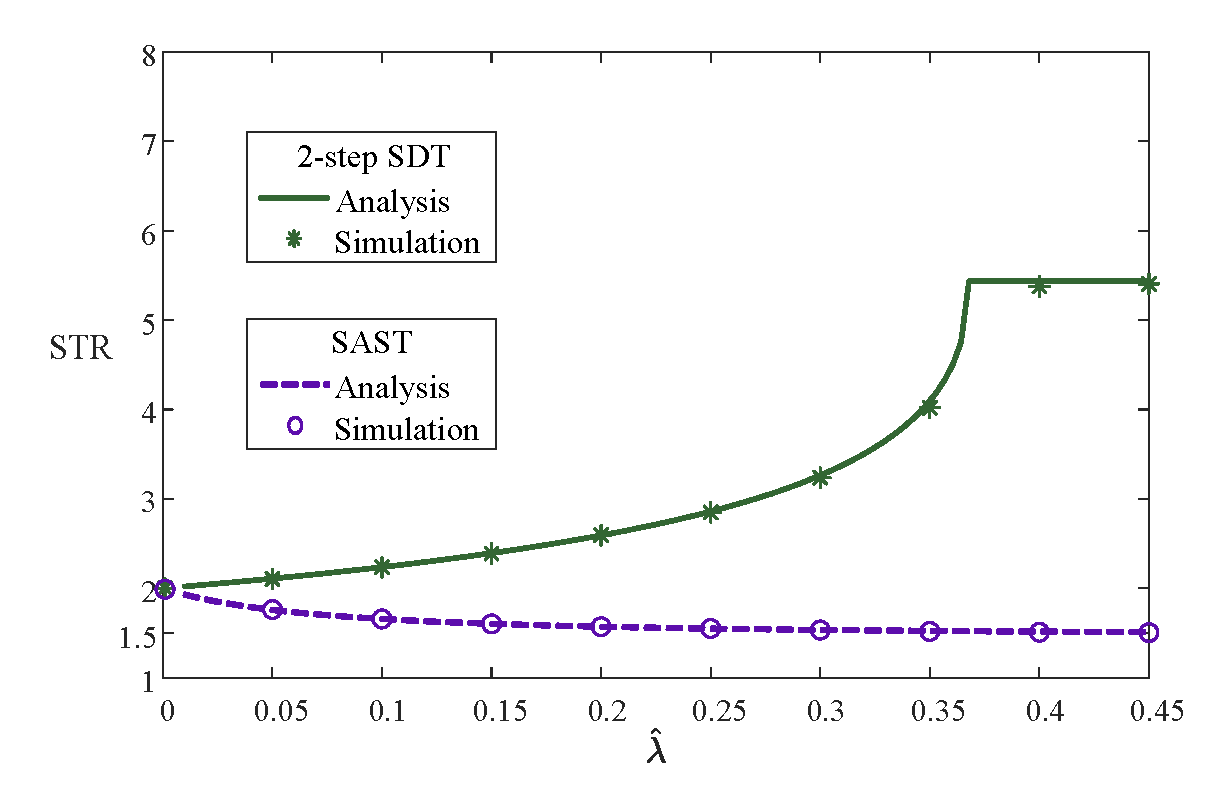
\includegraphics[width=\textwidth]{figure/chap3/str_vs_lambda_unsaturated.pdf}
		\caption{非饱和状态下的 STR 对比}
		\label{fig:str_unsat}
	\end{subfigure}
	\caption{SAST 与 2 步小数据传输方案的信令吞吐比性能对比，$n=100, s=1$}
	\label{fig:str_comparison}
\end{figure}

为直观展示两种方案性能差异，图 \ref{fig:str_comparison} 对比了不同负载条件下 STR 随传输概率 $q$ 的变化。
图~\ref{fig:str_sat} 给出了饱和状态下两种机制的信令吞吐比对比结果。在较小的接入概率 $q$ 区域内，SAST 方案的信令吞吐比明显低于 2 步小数据传输方案，其优势来源于信令分摊，即节点成功接入后可连续传输多个数据包，均摊了前导码与交互信令开销，从而降低单位数据信令消耗。该区域系统竞争较弱、碰撞概率较小，平均忙期长度 $\overline{B}$ 较高。理论上，当 $q \to 0$ 时，SAST 的单位数据信令开销可降至 2 步小数据传输方案的一半左右。
本质上，SAST 的性能提升以一定程度的信道访问公平性下降为代价，即一旦节点成功获得信道，其可在较长时间内持续占用信道并分摊信令开销，而其他节点则需等待下一轮竞争。
随着 $q$ 增大，参与竞争的节点增多，既降低接入成功率，又打断连续传输，使 $\overline{B}$ 缩短，削弱 SAST 的信令分摊能力。在这一过程中，SAST 的性能逐渐低于 2 步小数据传输方案。当 $q$ 继续增大时，连续传输难以维持，SAST 因接入失败频繁发送否定确认消息，其性能不再优于标准方案，甚至可能劣化。
另一方面，图~\ref{fig:str_unsat} 给出了非饱和状态下两种机制的信令吞吐比结果，可以观察到在稳定工作区间内，SAST 方案始终表现出更低的信令吞吐比。在非饱和条件下，整体竞争强度较低，碰撞概率小，使得成功接入后的连续传输过程能够稳定存在，可持续发挥信令开销分摊的优势。随着归一化输入率 $\hat{\lambda}$ 的增加，2 步小数据传输方案由于每个数据包均需独立完成接入过程，其信令开销随负载增加近似线性增长，而 SAST 由于能够在单次接入后完成多包传输，其信令开销增长更为缓慢，两者之间的差距明显。特别是在典型负载点附近，例如 $\hat{\lambda} = e^{-1}$，SAST 的信令吞吐比仅为对比方案的约 30\%。 

\section{本章小结}
\label{sec:sast_conclusion}

本章围绕 SAST 机制完成了三部分工作。一是基于信道与节点双视角建立休假排队模型，推导接入吞吐量与数据吞吐量关于网络参数的闭式表达式，并通过适当调整传输概率进一步优化这些吞吐指标。二是构建节点视角下的二维马尔可夫链，基于此分析了接入时延和数据包时延，为评估 SAST 机制的时延性能提供理论基础。三是将 5G 蜂窝网络中的 2 步小数据传输方案作为比较基准，推导了标准方案与本文 SAST 机制的信令吞吐比表达式，说明 SAST 机制在保持标准兼容性的同时具有信令开销优势。



        \newclearpage
        \chapter{面向 CSMA 协议的连续传输机制设计与性能分析}
\label{chapter4:CSMAST}

在前一章验证了连续传输机制在时隙 Aloha 协议中的性能增益后，本章进一步将其扩展至具备载波侦听能力的 CSMA 协议，提出 CSMAST 接入机制。与 Aloha 协议中基于等长离散时隙的建模假设不同，CSMA 协议中空闲、碰撞与成功传输的状态持续时长并不完全等同为单位时隙，从而给系统的理论建模带来了新的挑战。
为此，本章首先结合物理层侦听特性，对系统模型与协议流程进行重构；
在此基础上，引入休假排队理论方法，构建能够刻画状态持续时间非对称性的分析模型；
最后，基于所建模型推导饱和状态下的网络吞吐量与公平性两个性能指标，从而揭示 CSMAST 机制在该类网络环境下的特有性能演化规律。

\section{CSMAST 系统模型与机制描述}
\label{sec:csmast_system_model}

本章的研究工作建立在\ref{sec:general_system_model}节所述通用上行通信网络模型的基础之上，并针对 CSMA 协议中物理层与 MAC 层之间紧密交互的特性进行具体化建模与扩展。为探究连续传输机制在 CSMA 网络中的性能极限，本章进一步假设系统始终处于饱和状态，即网络中 $n$ 个同质节点的数据包缓冲队列始终非空，所有节点持续处于信道竞争状态。
下一小节将重点介绍 CSMA 网络中信道状态时长的非对称性；接着给出 CSMAST 协议的机制描述。

\subsection{信道状态与非对称时长特性}

在本章研究的 CSMA 网络中，时间轴仍被划分为连续的离散时隙，单位时隙长度定义为信号在网络中的最大传播时延与硬件侦听处理时延之和。同时，单个时隙也是系统可实现侦听的最小时间单位。
与时隙 Aloha 协议中各类信道状态固定占用一个单位时隙不同，CSMA 网络中的信道占用时长由具体信道状态决定，各类状态的持续时间呈现出明显的非对称性。
在 CSMA 网络中，节点通常处于持续侦听信道的状态，并根据信道是否空闲决定是否发起接入。当节点尝试接入信道时，其竞争结果可归纳为两类：成功传输与碰撞失败。由于两类事件对应的物理过程不同，其持续时间亦存在明显差异。
对于碰撞情形，受信号叠加效应及传播时延的影响，节点无法在发送瞬间立即检测到冲突。
本文假设在节点侧需要经过 $x$ 个时隙（$x \ge 1$）来检测到碰撞信号并终止无效传输，这意味着一次失败的竞争将导致信道被无效占用 $x$ 个传输时隙。
对于成功传输情形，节点在成功占用信道后完成数据包发送，其过程通常包括数据传输、传播时延以及接收端确认反馈等阶段，全程耗时 $y$ 个时隙，且通常满足 $y \ge x$。
此外，为确保信道感知的准确性，节点在每次信道占用结束后（无论是成功发送还是碰撞事件）都需经历一个额外的侦听时隙，以确认信道状态。

综上所述，从信道占用的视角来看，系统在时间域上可抽象为三类基本信道状态：
\begin{enumerate}
	\item 空闲状态（Idle, I），持续时间为 $\tau_I = 1$ 个时隙，表示当前信道未被任何节点占用，仅包含必要的侦听开销；
	\item 失败状态（Failure, F），持续时间为 $\tau_F = x + 1$ 个时隙，表示多节点并发接入导致传输失败，信道在碰撞被检测并恢复侦听之前处于无效占用状态；
	\item 成功状态（Success, S），持续时间为 $\tau_S = y + 1$ 个时隙，表示单节点成功完成数据包传输并获得确认反馈。
\end{enumerate}
这种状态时长的非对称性（即 $\tau_S \neq \tau_F \neq \tau_I$）是 CSMA 与 Aloha 协议的本质区别，也极大增加了后续理论建模的复杂度。

\subsection{CSMAST 协议机制描述}

在此异构时间模型下，本章提出了一种应用连续传输机制的 CSMA 增强方案，即 CSMAST。该协议的核心设计思想在于：通过一次成功的信道竞争，获取后续多次连续传输的机会，从而有效降低重复竞争所带来的接入开销。
从 CSMAST 机制流程上看，其遵循竞争接入、连续占用、退避重置的闭环逻辑。具体而言，当网络节点侦听到信道处于空闲状态（状态 I），或成功状态 S、失败状态 F 的最后一个时隙时，节点会在下一时隙起始时刻，依据预设概率 $q\in[0,1]$ 执行随机接入决策。
当节点根据随机接入策略选择不发送时，其将继续保持信道侦听状态，并在后续时隙中等待下一次接入机会；当节点选择发送时，则可能出现以下两种情况：
\begin{itemize}
	\item \textbf{成功传输与连续传输阶段}：节点发起传输且未发生冲突，顺利将队首数据包传输至基站，对应信道完整经历成功状态 $S$ 的前 $y$ 个时隙。随后，基站立即反馈确认消息，节点已知此时的信道状态，并进入连续传输阶段。注意，在这前 $y$ 个时隙内，信道处于繁忙状态，期间其他节点在侦听到信道繁忙后会保持静默，不会打断该节点的传输。
	为保证 CSMA 机制下先听后说的基本原则，并保留其他节点的接入机会，连续传输节点在发送后续数据包前仍需执行一次标准的信道侦听。然而，与初始接入不同，该节点可跳过后续随机接入流程，以概率 1 发送缓存中的下一个数据包，从而继续参与下一轮竞争。
	\item \textbf{碰撞冲突与退避重置机制}：节点在发送过程中（包括初始接入或连续传输阶段）与其他节点传输引发碰撞，信道进入状态 F 并经历前 $x$ 个时隙，基站返回否定确认消息或不返回有效反馈。所有参与冲突的节点（包括处于连续传输阶段的节点）均需立即终止当前传输，退避回到常规竞争态。在后续信道恢复空闲后，各节点将以概率 $q$ 重新发起接入。
\end{itemize}
相较于传统 CSMA 机制，CSMAST 不以消除竞争为目标，而是通过发送概率为 $1$ 的连续传输机制，使一次成功接入即可为后续多个数据包提供连续传输的机会，从而将初始空闲等待时长 $\tau_I$ 和碰撞损失时长 $\tau_F$ 的开销分摊至多个数据包。
随着连续传输长度的增加，单位数据包所承担的接入开销逐步下降，系统整体吞吐量也能得到提升。

从信道接入机制看，传统 CSMA 在单个数据包成功传输后即释放信道，节点重新进入侦听与随机退避过程，信道占用情况呈单包之间的离散分布；CSMAST 在保留载波侦听与碰撞退避规则不变的情况下，使成功节点在后续时隙经必要侦听后继续发送队列中的数据包，直到发生碰撞或队列清空，从而在物理层形成连续的信道占用区间。基于此，CSMAST 的核心区别在于不改变竞争判决过程，仅通过成功后的连续发送改变信道占用方式。

此外，CSMAST 机制在设计上区别于 IEEE 802.11e 中广泛采用的发送机会（TXOP）机制。TXOP 通常为节点分配一个固定的最大信道占用时间（MCOT），而 CSMAST 中的连续传输长度并非静态分配，而是由节点本地的队列积压状态与网络中其他节点的碰撞行为动态联合驱动的。当网络轻载时，节点可充分利用信道清空队列；当网络拥塞、发生并发碰撞时，连续传输会被即时打断并退回竞争态。这种动态反馈机制在缺乏中心调度的突发物联网场景中，具备更优的弹性与自适应能力。

\subsection{基于休假排队模型的 CSMAST 机制分析}
\label{subsec:csmast_mechanism_analysis}
\begin{figure}[t]
	\centering
	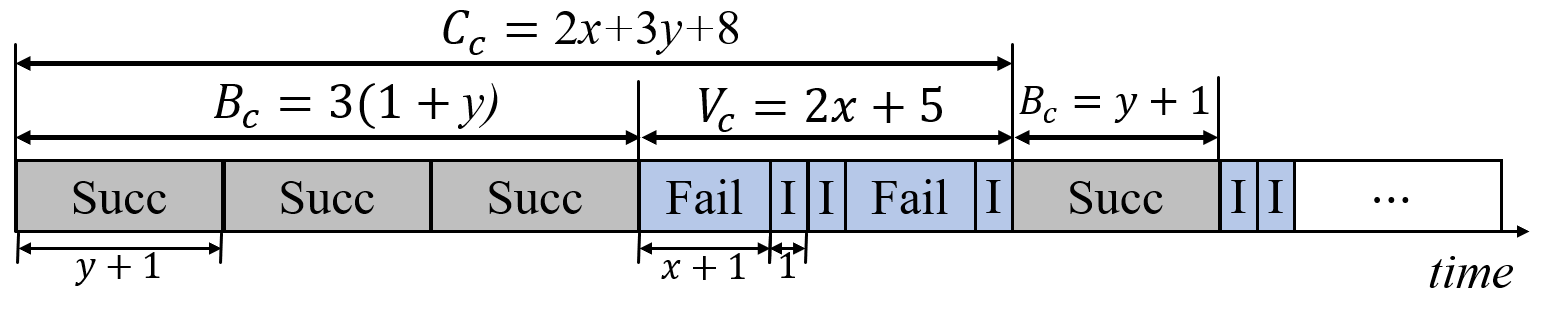
\includegraphics[width=0.9\textwidth]{figure/chap4/csmast_channel.png}
	\caption{CSMAST 方案中的信道状态演变示意图（$B$、$V_c$ 和 $C_c$ 分别表示信道的忙期、假期和周期时间）}
	\label{fig:csmast_channel}
\end{figure}

为了对 CSMAST 机制进行系统的定量分析，本小节引入离散时间休假排队理论作为建模基础。首先，我们将分析视角聚焦于信道的状态演变。从时间维度出发，CSMAST 网络中信道状态在连续占用与空闲/竞争阶段之间交替演化，呈现出明显的周期性特征。
图 \ref{fig:csmast_channel} 直观展示了 CSMAST 机制下的信道时序演化过程。基于上述信道时序演化过程的观察与抽象，对信道忙期与信道假期的概念作如下形式化定义：
\begin{itemize}
	\item \textbf{信道忙期 $B_c$}: 对应于图中连续出现的成功状态 S。在该阶段，某一节点成功占用信道，并通过连续传输机制持续发送数据包。从系统角度来看，该阶段对应于信道被有效利用以完成数据传输的过程。
	
	\item \textbf{信道假期 $V_c$}: 对应于图中碰撞状态 $F$ 与空闲状态 $I$ 的随机交替序列。
	该阶段刻画了上一忙期结束后，各节点为竞争下一次信道占用权所经历的接入过程。无论是由于多节点并发导致碰撞进入状态 $F$，还是由于无节点发送而处于状态 $I$，该阶段均对应于获取下一次成功接入所付出的时间开销与信令代价。
\end{itemize}
基于上述定义，将一次信道忙期与其后紧随的信道假期共同构成一个完整的信道周期，记为 $C_c$，即 $C_c = B_c + V_c$。
由于信道忙期由任一节点的成功接入所触发，且忙期一旦开始即由该节点独占信道并持续传输，因此从统计特性上看，信道层面的忙期与单节点视角下的忙期在概率分布上是等价的。为简化符号表示，后续分析中统一使用 $B$ 表示信道忙期。下文使用 $\overline{B} \triangleq \mathbb{E}[B]$ 和 $\overline{V}_c \triangleq \mathbb{E}[V_c]$ 分别表示信道忙期与信道假期的平均持续时长。具体的概率分布推导及性能指标计算将在下一节中进一步展开。

\section{基于休假排队理论的建模分析}
在进行具体推导之前，本节首先定义三个常用概率。根据第 ~\ref{subsec:channel_vacation_analysis}~节的分析，在饱和网络条件下，当节点数量 $n$ 较大且接入概率 $q$ 较小时，系统中的接入请求总数可近似建模为参数为 $\theta = nq$ 的泊松随机变量。在任意空闲时隙中，网络内发起接入请求的节点数量刻画了系统的瞬时竞争程度，并决定了下一时隙的信道状态转移。基于此，定义如下三个概率：
\begin{itemize}
	\item $p_0 = e^{-\theta}$：表示无节点发起接入请求的概率，即信道保持空闲状态。
	\item $p_1 = \theta e^{-\theta}$：表示恰有一个节点发起接入请求的概率，此时该节点成功占用信道并完成一次成功传输。
	\item $p_2 = 1 - p_0 - p_1$：表示至少有两个节点同时发起接入请求的概率，此时发生碰撞，对应信道进入失败状态。
\end{itemize}
下文将充分使用这三个概率，在所建立的休假排队模型中详细阐述忙期和假期分布规律。

\subsection{信道忙期 $B$ 分布的推导分析}
\label{subsec:B_analysis}
与第~\ref{chapter3:SAST}章所述的 SAST 机制类似，CSMAST 中的信道忙期分布取决于两个关键因素：一是当前占用节点是否持续发送，二是是否有其他节点发起接入请求并引发竞争。
在饱和网络假设下，当前已经成功接入的节点缓存始终非空，因此其在完成当前数据包传输后，将以概率 $1$ 持续发送后续数据包。
这意味着，信道忙期一旦开始，其终止不再依赖于发送节点的行为，而仅由其他节点发起接入请求所引发的碰撞事件所决定。
具体而言，一个信道忙期由若干个连续的成功传输状态 $S$ 构成，每个成功状态的持续时间为 $\tau_S$。在每个成功状态结束前的最后一个时隙（即侦听时隙）内，其余 $n-1$ 个节点对信道进行侦听，并据此判断得出信道将转入空闲态，从而可能发起新的接入请求。
根据前述的泊松近似，在该侦听时隙之后的下一时隙，网络中无其他节点发起接入请求的概率为$p_0 = e^{-\theta}$。此时系统可能出现以下两种情况：
\begin{itemize}
	\item 以概率 $p_0$，无其他节点发起接入请求，当前占用节点得以继续传输，信道状态由成功状态 $S$ 延续为新的成功状态，忙期持续。
	\item 以概率 $1 - p_0$，至少有一个其他节点发起接入请求，与当前节点的下一次传输发生冲突并引发碰撞，信道状态由成功状态 $S$ 转变为失败状态 $F$，从而终止当前忙期。
\end{itemize}
基于上述状态转移机制，忙期内连续成功传输的次数可建模为服从参数为 $1 - p_0$ 的几何分布，其中终止事件对应于碰撞的发生。考虑到每次成功传输的持续时间固定为 $\tau_S$，并且假设各成功状态之间的延续与终止事件相互独立，信道忙期的期望长度 $\overline{B}$可表示为：
\begin{equation}
	\overline{B} = \frac{\tau_S}{1 - p_0} = \frac{\tau_S}{1 - e^{-nq}}.
\end{equation}
进一步地，为评估系统服务过程的稳定性并支撑后续公平性分析，需要刻画信道忙期长度的波动特性。
基于前述几何分布建模结果，利用其方差表达式，信道忙期长度的方差 $\sigma_B^2$ 可表示为：
\begin{equation}
	\sigma^2_B = \tau_S^2 \cdot \frac{p_0}{(1 - p_0)^2} = \frac{ \tau_S^2 e^{-nq} }{(1 - e^{-nq})^2}.
\end{equation}
上述期望与方差从平均水平与波动程度两方面刻画了信道忙期特性。本质上，两者均由概率 $p_0$ 所主导。当 $p_0$ 较大时，节点在成功接入后更容易维持连续传输，平均占用信道的时间增加且波动性增强；反之，当 $p_0$ 较小时，忙期频繁终止，占用信道的时间更短且分布更集中。


\subsection{信道假期 $V_c$ 分布的推导与分析}
\label{subsec:Vc_analysis}
\begin{figure}[t]
	\centering
	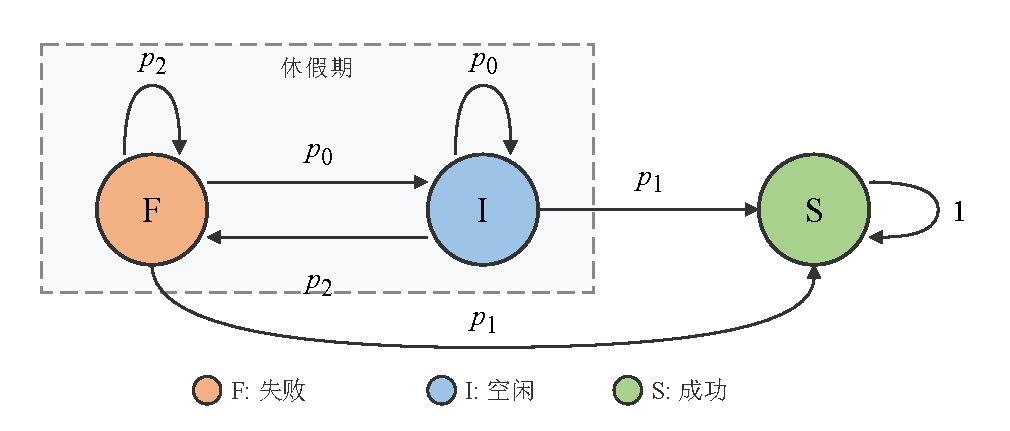
\includegraphics[width=0.95\textwidth]{figure/chap4/markov_model.pdf}
	\caption{描述信道假期 $V_c$ 内状态转移过程的吸收马尔可夫链模型（状态 F 和 I 为可转移态，状态 S 为吸收态）}
	\label{fig:csmast_markov_absorption}
\end{figure}

相较于仅包含成功传输的信道忙期，信道假期 $V_c$ 的演化更为复杂。
假期通常始于一次导致忙期终止的碰撞事件，此后信道在空闲与碰撞失败状态之间随机切换，直至某一时隙产生唯一成功传输，从而结束当前假期并开启新的信道忙期。
另一方面，空闲状态时长 $\tau_I$ 与碰撞状态时长 $\tau_F$ 并不相等，一般情况下 $\tau_F > \tau_I$。
因此，假期总时长不仅取决于状态转移情况，还与系统在不同状态下的驻留时间密切相关。
由于状态持续时间的非均匀性，基于独立同分布假设的几何分布模型难以准确刻画该过程的统计特性。
为推导信道假期分布特性，本文将在一个信道假期 $V_c$ 内，信道状态的演化过程建模为一个具有吸收态的马尔可夫链。该模型通过引入吸收态描述假期的终止事件，并刻画空闲状态与碰撞失败状态之间的随机转移关系，其状态转移结构如图 \ref{fig:csmast_markov_absorption} 所示。为形式化描述上述吸收马尔可夫链模型，本文首先构建其状态空间与转移概率矩阵，具体定义如下：

\begin{itemize}
	\item 模型包含三个状态。其中，碰撞状态 F 和空闲状态 I 构成瞬时状态集合，表示假期仍在持续；成功状态 S 是唯一的吸收态，一旦进入该状态，意味着某个节点竞争成功，假期结束并转入忙期。
	\item 在任意非忙期时隙，即状态 I 的时隙或状态 F 的最后一个侦听时隙，网络中发起接入请求总次数决定了下一时刻的状态跳转，有以下三个情况：
	\begin{enumerate}
		\item 无任何节点接入的概率为 $p_0 = e^{-\theta}$，此时信道保持静默，并进入空闲状态 I。
		\item 恰有一个节点发起接入的概率为 $p_1 = \theta e^{-\theta}$，此时信道进入成功状态 S，过程被吸收。
		\item 有多个节点同时接入的概率为 $p_2 = 1 - p_0 - p_1$，此时发生碰撞，信道进入碰撞状态 F。
	\end{enumerate}
\end{itemize}
基于上述转移逻辑，其状态转移概率矩阵 $\mathbf{P}$ 可表示为如下的标准分块形式：
\begin{equation}
	\mathbf{P} = 
	\begin{pmatrix}
		p_2 & p_0 & p_1 \\
		p_2 & p_0 & p_1 \\
		0 & 0 & 1
	\end{pmatrix}
	=
	\begin{pmatrix}
		\mathbf{T} & \mathbf{R} \\
		\mathbf{0} & \mathbf{I}
	\end{pmatrix},
\end{equation}
其中，$\mathbf{T} = \begin{pmatrix} p_2 & p_0 \\ p_2 & p_0 \end{pmatrix}$ 描述了瞬态之间的转移概率，$\mathbf{R} = \begin{pmatrix} p_1 \\ p_1 \end{pmatrix}$ 描述了进入吸收态的概率。
根据马尔可夫吸收理论\cite{2008_Markov_absorb}，相关性能指标的计算依赖于基本矩阵 $\mathbf{N} = (\mathbf{I} - \mathbf{T})^{-1}$。其中，矩阵 $\mathbf{N}$ 中的元素 $N_{ij}$ 表示过程从瞬时状态 $i$ 开始，在被吸收之前访问到瞬时状态 $j$ 的期望次数。本节中，矩阵 $\mathbf{N}$ 的行、列索引按顺序分别对应状态 F 和状态 I。
首先计算矩阵 $(\mathbf{I} - \mathbf{T})$：
\begin{equation}
	\mathbf{I} - \mathbf{T} = 
	\begin{pmatrix} 1 & 0 \\ 0 & 1 \end{pmatrix} - \begin{pmatrix} p_2 & p_0 \\ p_2 & p_0 \end{pmatrix} 
	= \begin{pmatrix} 1-p_2 & -p_0 \\ -p_2 & 1-p_0 \end{pmatrix}.
\end{equation}
其行列式为 $\det(\mathbf{I} - \mathbf{T}) = (1-p_2)(1-p_0) - p_0 p_2 $。
结合概率归一化关系 $p_0 + p_1 + p_2 = 1$，求解基本矩阵 $\mathbf{N}$为
\begin{equation}
	\mathbf{N} = \frac{1}{p_1} \begin{pmatrix} 1-p_0 & p_0 \\ p_2 & 1-p_2 \end{pmatrix}.
\end{equation}

在饱和网络条件下，信道假期均由碰撞状态触发，因而仅需关注从碰撞状态 $F$ 出发的期望访问次数。根据基本矩阵定义，$N_{FF} = (1-p_0)/p_1$ 表示在吸收之前访问碰撞状态 $F$ 的期望次数，对应假期内经历的平均碰撞次数，$N_{FI} = p_0/p_1$ 为空闲状态 $I$ 的期望次数，对应假期内经历的平均空闲次数。
令列向量 $\boldsymbol{\mu} = [\tau_F, \tau_I]^T$ 表示各瞬时状态的单次驻留时长，则从各瞬态出发至吸收态的期望总时间向量 $\mathbf{F}$ 可表示为 $\mathbf{F} = \mathbf{N} \boldsymbol{\mu}$。
取向量 $\mathbf{F}$ 的第一个分量，对应初始状态 F。代入 $p_0 = e^{-\theta}$、$p_1 = \theta e^{-\theta}$ 以及 $\theta = nq$，即可得到信道假期的期望长度为：
\begin{equation}
	\overline{V}_c = [\mathbf{F}]_1 = [\mathbf{N} \boldsymbol{\mu}]_1 = \frac{1-p_0}{p_1}\tau_F + \frac{p_0}{p_1}\tau_I = \frac{(1 - e^{-nq})\tau_F + e^{-nq}\tau_I}{nq e^{-nq}}.
\end{equation}

为了分析公平性，还需计算假期长度 $V_c$ 的二阶统计量。根据吸收马尔可夫链理论，从各瞬态出发至吸收态的总时间二阶矩向量 $\mathbf{G}$ 满足
\begin{equation}
	\mathbf{G} = \mathbf{N} ( \mathbf{m}_2 + 2 \cdot \text{diag}(\boldsymbol{\mu}) \cdot \mathbf{T} \mathbf{F} ),
\end{equation}
其中 $\mathbf{m}_2 = [\tau_F^2, \tau_I^2]^T$ 为各瞬态单次驻留时间的二阶矩向量，$\text{diag}(\boldsymbol{\mu})$ 为以 $\boldsymbol{\mu}$ 为对角元素的对角矩阵。
提取向量 $\mathbf{G}$ 的第一个分量，可以得到从状态 F 出发至吸收态的假期长度的二阶原点矩 $\mathbb{E}[V_c^2] = \mathbf{G}_1$。因此，信道假期的方差 $\sigma^2_{V_c}$ 由公式 $\sigma^2_{V_c} = \mathbf{G}_1 - (\overline{V}_c)^2$ 给出：
\begin{equation}
	\sigma^2_{V_c} =
	\frac{\left[(1 - p_0)\tau_F + p_0\tau_I\right]^2}{p_1^2} - \frac{(1 - p_0)\tau_F^2 + p_0\tau_I^2}{p_1}.
\end{equation}


\subsection{信道周期 $C_c$ 与节点周期 $C$ 的推导与分析}
\label{subsec:cycle_analysis}

基于前文对信道忙期 $B$ 和信道假期 $V_c$ 的独立分析，下面推导完整信道周期 $C_c$ 以及节点周期 $C$ 的统计特性。这一推导能够表征系统的时间演化规律，周期长度的方差将直接决定系统的短期公平性性能。

首先分析信道周期 $C_c$ 的均值与方差。根据休假排队模型定义，一个完整的信道周期 $C_c$ 由一个忙期 $B$ 和随后的一个假期 $V_c$ 构成，满足关系式 $C_c = B + V_c$。
在 CSMAST 机制下，信道忙期长度取决于当前占用节点的连续发送意愿以及碰撞发生概率，信道假期长度取决于碰撞和空闲状态跳转。需要注意的是，假期开始意味着上一次忙期的状态记忆被完全重置，碰撞会使得所有节点重新参与信道竞争，因此在系统平稳情况下，随机变量 $B$ 与 $V_c$ 可被视为相互独立。

依据概率论中独立随机变量和的基本性质，信道周期的均值$\overline{C}_c$和方差$\sigma^2_{C_c}$ 可由其组成部分的统计量线性叠加得到，即
\begin{equation}
	\overline{C}_c = \overline{B} + \overline{V}_c,
\end{equation}
\begin{equation}
	\sigma^2_{C_c} = \sigma^2_B + \sigma^2_{V_c}.
\end{equation}
式中$\overline{B}$和$\sigma^2_B$在\ref{subsec:B_analysis}节已经得出，$\overline{V}_c$和$\sigma^2_{V_c}$在\ref{subsec:Vc_analysis}节中推导。该结果完整刻画了信道资源在占用状态与争夺状态之间切换的时间特征。

然后分析节点周期$C$及其方差$\sigma^2_C$的映射关系。
为刻画节点间的公平性特征，本文将分析视角由信道转向单节点。与第~\ref{chapter3:SAST}章类似，定义节点周期 $C$ 为某一特定节点两次连续接入信道并开启忙期之间的时间间隔。
在包含 $n$ 个同质节点的饱和网络中，各节点具有一致的统计特性，且传输概率 $q$ 相同。每一次成功接入对应一个完整的信道周期 $C_c$，并以相同概率 $1/n$ 归属于任意一个节点。对于某一指定节点而言，其成功接入信道的过程可等效视为在信道周期序列上进行一次以 $1/n$ 为采样概率的随机稀疏采样过程。
换言之，对于任一给定节点，其平均需要经历约 $n$ 个信道周期后才能成功接入信道。因此，节点周期的均值 $\overline{C}$ 与信道周期均值 $\overline{C}_c$ 之间满足如下线性比例关系：
\begin{equation}
	\overline{C} = n \overline{C}_c.
\end{equation}

结合更新过程理论中关于点过程稀疏化的相关结论，当网络节点规模 $n$ 较大且信道周期之间的相关性较弱时，节点周期的方差 $\sigma^2_C$ 与信道周期方差 $\sigma^2_{C_c}$ 之间存在近似关系：
\begin{equation}
	\label{eq:node_cycle_variance}
	\sigma^2_C \approx n^2 \sigma^2_{C_c} - (1 - n)n\overline{C}_c \approx n^2 \sigma^2_{C_c}.
\end{equation}
上式中的近似 $\sigma^2_C \approx n^2 \sigma^2_{C_c}$ 是基于 $n$ 较大时第一项占主导地位而得到的。

该结论表明，节点周期的波动性会随着信道周期的波动而发生变化，并被网络规模 $n$ 的平方放大。结合前文分析结论，当传输概率 $q$ 取值较小时，信道忙期的方差 $\sigma^2_B$ 数值较大，存在节点长时占用信道的可能，进而导致信道周期方差 $\sigma^2_{C_c}$ 增大，再通过上述方差映射关系放大节点周期的波动幅度。这种较大的服务间隔波动，从数学上揭示了 CSMAST 机制在提升系统吞吐量的同时可能牺牲节点间公平性的内在原因，也为下一节推导 Jain 公平性指数奠定了理论基础。


\section{吞吐量与公平性指标的推导与分析}
\label{sec:csmast_performance}

基于前文构建的休假排队模型及信道与节点周期的统计特性，本节将推导 CSMAST 网络在饱和状态下的两个核心性能指标，即网络吞吐量与 Jain 公平性指数。这不仅能够定量评估该机制的传输效率，还能揭示连续传输策略在系统效率与用户公平之间的内在权衡关系。

\subsection{网络吞吐量指标的推导与分析}

网络吞吐量 $\lambda^{net}_{out}$ 定义为单位时间内信道成功传输的有效数据数量，以包/时隙为单位。
在计算该指标时，必须考虑成功状态 S 的特殊性。虽然成功状态持续 $\tau_S$ 个时隙，但其中仅有 $y$ 个时隙用于实际数据包传输，剩余的 1 个时隙被用于必要的信道侦听。因此，信道忙期 $\overline{B}$ 并不能完全代表有效吞吐时间，需引入修正因子 $\frac{\tau_S - \tau_I}{\tau_S} = \frac{y}{y+1}$。
结合前文推导的 $\overline{B}$ 和 $\overline{V}_c$ 表达式，饱和状态下的网络吞吐量可表示为：
\begin{equation}
	\lambda^{net}_{out} = \frac{\tau_S - \tau_I}{\tau_S} \cdot \frac{\overline{B}}{\overline{B} + \overline{V}_c}.
\end{equation}
将 $p_0 = e^{-nq}$ 及 $\overline{B}, \overline{V}_c$ 关于网络参数的表达式代入，得到 CSMAST 网络吞吐量的闭式表达式为
\begin{equation}
	\label{eq:throughput_csmast}
	\lambda^{net}_{out} = \frac{nq(\tau_S - \tau_I)}{nq\tau_S + e^{nq}(1 - e^{-nq})^2 \tau_F + (1 - e^{-nq})\tau_I}.
\end{equation}
基于上述结果，进一步给出 CSMAST 吞吐量极限的如下定理：

\begin{theorem}[CSMAST 最大网络吞吐量]
	\label{thm:csmast_max_throughput}
	在饱和状态下，CSMAST 的网络吞吐量是关于参数 $nq$ 的单调递减函数。其理论最大吞吐量在接入概率 $q \to 0$ 时取得：
	\begin{equation}
		\lambda_{max}^{net} = \lim_{nq \to 0} \lambda^{net}_{out} = \frac{\tau_S - \tau_I}{\tau_S + \tau_I}.
	\end{equation}
\end{theorem}

\begin{proof}
	对于单调性，令 $x = nq$。饱和网络吞吐量可表示为 $g(x) = \frac{C x}{x \tau_S + F(x)}$，其中 $C = \tau_S - \tau_I > 0$，分母中的信道假期相关项为 $F(x) = \tau_F e^x (1 - e^{-x})^2 + \tau_I (1 - e^{-x})$。
	对 $g(x)$ 求导，其导数的符号完全取决于分子部分的判别式 $T(x) \triangleq F(x) - x F'(x)$。将 $F(x)$ 及其导数代入，并利用基本不等式 $1 - e^{-x} \le x$ 和 $e^{-x} \le 1$（对于 $x > 0$），可以证明在通常的系统参数设定下（即 $\tau_F \ge \tau_I$），判别式满足 $T(x) \le 0$。
	由于 $g'(x)$ 与 $T(x)$ 同号，因此 $g'(x) \le 0$ 在定义域内恒成立。这证明了 CSMAST 的网络吞吐量是关于 $nq$ 的单调递减函数。
	
	对于最值，利用洛必达法则对式 (\ref{eq:throughput_csmast}) 在 $nq \to 0$ 处求极限。注意到分母中 $e^{nq}(1-e^{-nq})^2 \approx (nq)^2$ 为高阶小量，主要项为 $(1-e^{-nq})\tau_I \approx nq \tau_I$。分子近似为 $nq(\tau_S - \tau_I)$。分子分母约去 $nq$ 后，第一项 $nq\tau_S$ 趋于 0，剩余部分即为极限值 $\frac{\tau_S - \tau_I}{\tau_S + \tau_I}$。
\end{proof}

定理 \ref{thm:csmast_max_throughput} 给出了 CSMAST 的最大理论吞吐量。以典型参数配置 $\tau_S=5, \tau_F=3, \tau_I=1$ 为例，CSMAST 的理论极限吞吐量可达 $4/6 \approx 0.667$，而相同参数下的经典 CSMA 仅能达到约 0.518，对应约 28.8\% 的吞吐量提升。这表明 CSMAST 通过连续传输机制，将空闲侦听 $\tau_I$ 和碰撞退避 $\tau_F$ 的时间成本分摊到连续多个数据包传输过程中，从而降低单位数据包的平均接入成本。

值得指出的是，本文所构建的基于吸收马尔可夫链的休假排队模型具有良好的扩展性与统一性。CSMAST 机制的性能增益本质上来源于连续传输机制增加了平均信道忙期 $\overline{B}$。作为该模型的一种特例，若在分析中约束节点在完成单个数据包传输后必须立即释放信道，即将忙期退化为确定性常数 $\overline{B} = \tau_S$，则所建立的模型可自然退化为对经典 CSMA 协议的性能刻画。在该情形下，系统不再具备连续占用信道的能力，其信道接入行为与传统 CSMA 机制一致。因此，经典 CSMA 协议可视为本文模型在特定参数约束下的一个退化情形。
关于经典 CSMA 在本章相同模型框架下的详细推导及最大吞吐量计算，详见附录\ref{app:classic_csma}。综上，该理论联系不仅验证了所提模型在不同接入机制下的一致性与通用性，同时也为后续性能对比分析提供了统一的数学基准。

\subsection{公平性指标的推导与分析}

尽管连续传输机制提升了系统吞吐量，但其一旦接入便持续占用信道的特性不可避免地对节点间的公平性构成挑战。为了量化这一影响，本节采用短期 Jain 公平性指数 $J_T$ 作为评估指标，并基于前文推导其闭式解。

设 $\lambda_{out, i}^T$ 为节点 $i$ 在给定观测时间窗 $T$ 内的短期归一化吞吐量。Jain 公平性指数定义为
\begin{equation}
	J_T = \frac{\left(\sum_{i=1}^n \lambda_{out, i}^T\right)^2}{n \sum_{i=1}^n \left(\lambda_{out, i}^T\right)^2}.
\end{equation}
由于网络中所有节点是同质的，$\lambda_{out, i}^T$ 可视为一组独立同分布的随机变量。根据大数定律，当节点数量 $n$ 足够大时，上述定义表达式可以写成
\begin{equation}
	\label{eq:jain_moment_form}
	J_T \approx \frac{\mathbb{E}[\lambda_{out, i}^T]^2}{\mathbb{E}[(\lambda_{out, i}^T)^2]} = \frac{1}{1 + \frac{\text{Var}(\lambda_{out, i}^T)}{\mathbb{E}[\lambda_{out, i}^T]^2}}.
\end{equation}
因此，求解 $J_T$ 的关键在于推导短期内节点吞吐量的均值 $\mathbb{E}[\lambda_{out, i}^T]$ 和方差 $\text{Var}(\lambda_{out, i}^T)$。

在 CSMAST 饱和网络中，节点 $i$ 的成功接入过程构成一个更新过程。令 $N_i(T)$ 表示节点 $i$ 在时间 $T$ 内成功完成的节点周期数，即节点经历的忙期次数。节点的短期吞吐量可表示为单位时间内传输的数据包总量：
\begin{equation}
	\lambda_{out, i}^T \approx \frac{N_i(T) \cdot \overline{B}}{T}.
\end{equation}
当观测时间 $T$ 充分长，即 $T \gg \overline{C}$ 时，根据更新理论的渐近性质\cite{1996_Gausian}，计数过程 $N_i(T)$ 近似服从正态分布，其均值和方差分别为：
\begin{equation}
	\mathbb{E}[N_i(T)] \approx \frac{T}{\overline{C}}, \quad \text{Var}(N_i(T)) \approx \frac{\sigma^2_C}{\overline{C}^3} T.
\end{equation}
基于此，短期吞吐量的统计特征总结为：
\begin{equation}
	\mathbb{E}[\lambda_{out, i}^T] = \frac{\overline{B}}{\overline{C}}, \quad \text{Var}(\lambda_{out, i}^T) = \left( \frac{\overline{B}}{T} \right)^2 \times \text{Var}(N_i(T)) = \frac{\overline{B}^2 \sigma^2_C}{\overline{C}^3 T}.
\end{equation}
将上述均值和方差代入式 (\ref{eq:jain_moment_form})，化简并展开可得到 Jain 公平性指数的闭式表达式：
\begin{equation}
	\label{eq:jain_explicit}
	J_T \approx \frac{1}{1 + \frac{n}{T} \cdot \frac{n^2 q^2 \tau_S^2 e^{nq} + (e^{nq}-1)^2 \tau_F^2 + 2(e^{nq}-1)\tau_F \tau_I + \tau_I^2}{nq \tau_S e^{nq} + (e^{nq}-1)^2 \tau_F + (e^{nq}-1)\tau_I}}.
\end{equation}
\section{仿真验证与结果分析}
\label{sec:simulation_results}


本节通过蒙特卡洛仿真从三个层面验证前文结论：理论一致性、与经典 CSMA 的对比增益、以及机制层面的性能权衡。仿真平台基于 MATLAB 构建，严格遵循第 4.1 节定义的异构时隙结构与碰撞信道模型。在所有仿真中，网络处于饱和状态，节点仅在侦听到信道可用时才以概率 $q$ 在下一时隙发起接入。
在仿真中，网络吞吐量按
$\lambda^{net}_{out}=\frac{N_{succ}(\tau_S-\tau_I)}{T}$
计算，其中 $N_{succ}$ 表示观测窗口内总体成功接入次数，$T$ 为总仿真时长。
短期公平性由各节点短期吞吐量按 Jain 指数标准定义计算，即
$J_T=\frac{\left(\sum_{i=1}^{n}\lambda_{out,i}^{T}\right)^2}{n\sum_{i=1}^{n}(\lambda_{out,i}^{T})^2}$。
其中节点 $i$ 的短期吞吐量按
$\lambda_{out,i}^{T}=\frac{N_{succ,i}(\tau_S-\tau_I)}{T}$
计算，$N_{succ,i}$ 表示节点 $i$ 在观测窗口内的成功数据包数量。
% 除非另有说明，本节采用基准参数 $n=100$、$T=10^6$、$x=2$、$y=4$，即 $\tau_I=1,\tau_F=3,\tau_S=5$，并在图注中明确对应的观测窗口。

\subsection{网络吞吐量 $\lambda^{net}_{out}$ 的仿真验证与分析}

\begin{figure}[t]
	\centering
	\begin{subfigure}{0.49\textwidth}
		\centering
		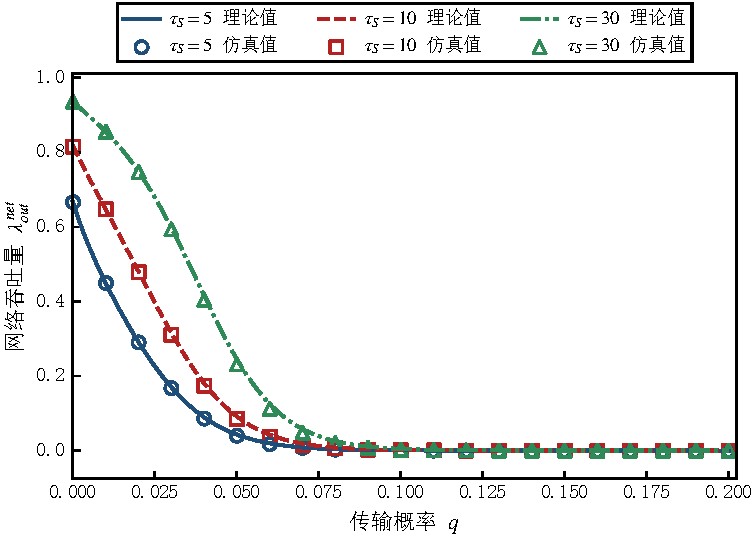
\includegraphics[width=\linewidth]{figure/chap4/thu_vs_q_CSMAST_multi_taus.pdf}
		\caption{不同 $\tau_S$ 下 $\lambda^{net}_{out}$ 随接入概率 $q$ 的变化情况}
		\label{fig:csmast_throughput_vs_q_taus}
	\end{subfigure}
	\hfill
	\begin{subfigure}{0.49\textwidth}
		\centering
		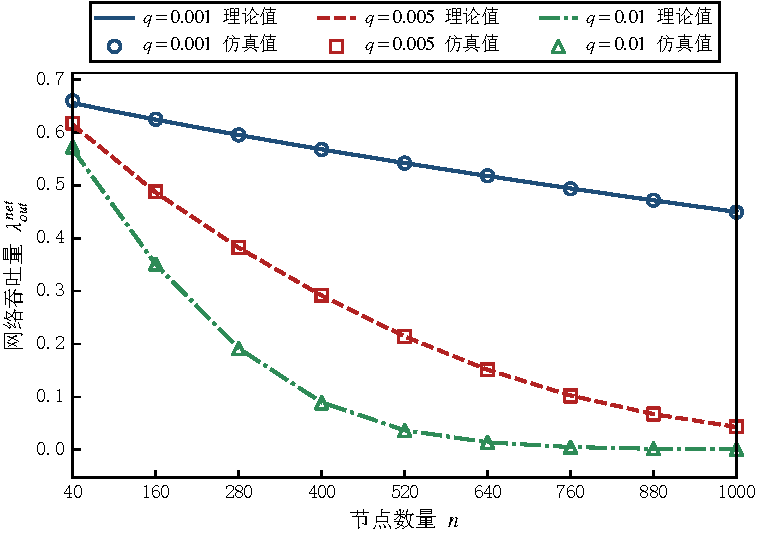
\includegraphics[width=\linewidth]{figure/chap4/thu_vs_n_CSMAST_multi_q.pdf}
		\caption{网络吞吐量 $\lambda^{net}_{out}$ 随节点数量 $n$ 的变化情况}
		\label{fig:csmast_throughput_vs_n}
	\end{subfigure}
	\caption{CSMAST 机制下吞吐量随系统参数变化情况}
	\label{fig:csmast_throughput_group}
\end{figure}

图 \ref{fig:csmast_throughput_vs_q_taus} 给出了不同成功传输时长 $\tau_S$ 条件下，网络吞吐量 $\lambda^{net}_{out}$ 随接入概率 $q$ 变化的曲线趋势。实验参数设置为节点数 $n=100$、碰撞时长 $\tau_F=3$、空闲时长 $\tau_I=1$、观测时间窗口 $T=10^6$，并取 $\tau_S\in\{5,10,30\}$。结果显示，在相同接入概率 $q$ 下，$\tau_S$ 越大，吞吐量曲线整体越高。该现象说明成功传输阶段越长，单位成功发送的数据包所经历的时间开销越低，从而提升了网络吞吐量。随着 $q$ 增大，三组曲线均持续下降，原因在于并发接入概率上升导致碰撞频率增加，有效传输时间占比下降。在较大 $q$ 区域，曲线间距逐步收敛，表明系统性能主要受高冲突过程主导，$\tau_S$ 带来的增益受到削弱。理论曲线与仿真结果在全区间内保持一致，验证了理论对该参数变化规律的准确性。

\begin{figure}[t]
	\centering
	\begin{subfigure}{0.49\textwidth}
		\centering
		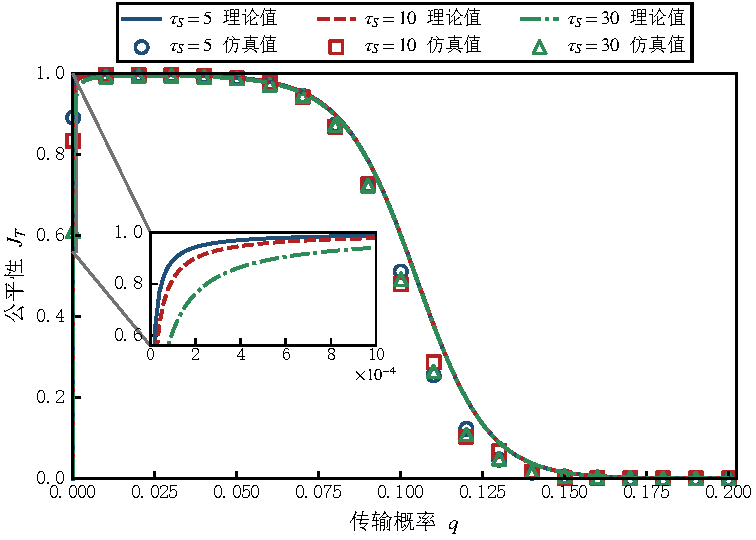
\includegraphics[width=\linewidth]{figure/chap4/jt_vs_q_CSMAST_multi_taus.pdf}
		\caption{不同 $\tau_S$ 下公平性 $J_T$ 随接入概率 $q$ 的变化情况}
		\label{fig:csmast_jain_vs_q_taus}
	\end{subfigure}
	\hfill
	\begin{subfigure}{0.49\textwidth}
		\centering
		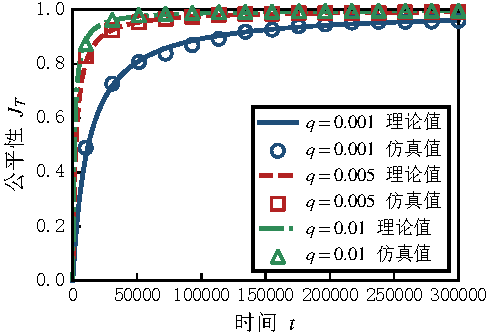
\includegraphics[width=\linewidth]{figure/chap4/jt_vs_t_CSMAST_multi_q.pdf}
		\caption{不同 $q$ 下短期公平性 $J_T$ 随观测时间窗口 $T$ 的变化情况}
		\label{fig:csmast_jain_vs_t_multi_q}
	\end{subfigure}
	\caption{CSMAST 机制下公平性关于系统参数的变化情况}
	\label{fig:csmast_fairness_group}
\end{figure}

为考察网络规模影响，图~\ref{fig:csmast_throughput_vs_n} 给出了不同接入概率 $q$ 条件下网络吞吐量 $\lambda^{net}_{out}$ 随节点数量 $n$ 变化的趋势。实验参数设置为成功传输时长 $\tau_S=5$、碰撞时长 $\tau_F=3$、空闲时长 $\tau_I=1$、观测时长 $T=10^6$。结果显示，在任一固定 $q$ 下，$n$ 增大将提高总体竞争强度，并增加碰撞与侦听带来的时间开销，使吞吐量整体下降；在任一固定 $n$ 下，较小 $q$ 往往对应更高吞吐量，但也会伴随更明显的公平性代价。
% 理论与仿真曲线的总体一致性说明该模型在不同负载区间均具有较好解释力。

\subsection{公平性 $J_T$ 的仿真验证与分析}


图 ~\ref{fig:csmast_jain_vs_q_taus} 进一步给出了不同 $\tau_S$ 下短期公平性 $J_T$ 随接入概率 $q$ 的变化趋势。实验参数设置为节点数 $n=100$、碰撞时长 $\tau_F=3$、空闲时长 $\tau_I=1$，观测时长 $T=10^6$，并取 $\tau_S\in\{5,10,30\}$。该图表明，在低接入概率区间，$\tau_S$ 越大，$J_T$ 越低，说明连续忙期越长，节点间短时服务差异越明显。随着 $q$ 增大，碰撞对信道连续占用的中断效应增强，增加了信道占用权在节点之间的轮转，$J_T$ 因而逐步上升。进入高接入概率区间后，$J_T$ 逐渐下降并且不同 $\tau_S$ 下的公平性曲线逐渐收敛，说明公平性主要由竞争过程主导，而忙期长度差异的影响相对减弱。
% 理论曲线与仿真点在全区间保持一致，进一步验证了第 4.3 节公平性模型的有效性。

\begin{figure}[t]
	\centering
	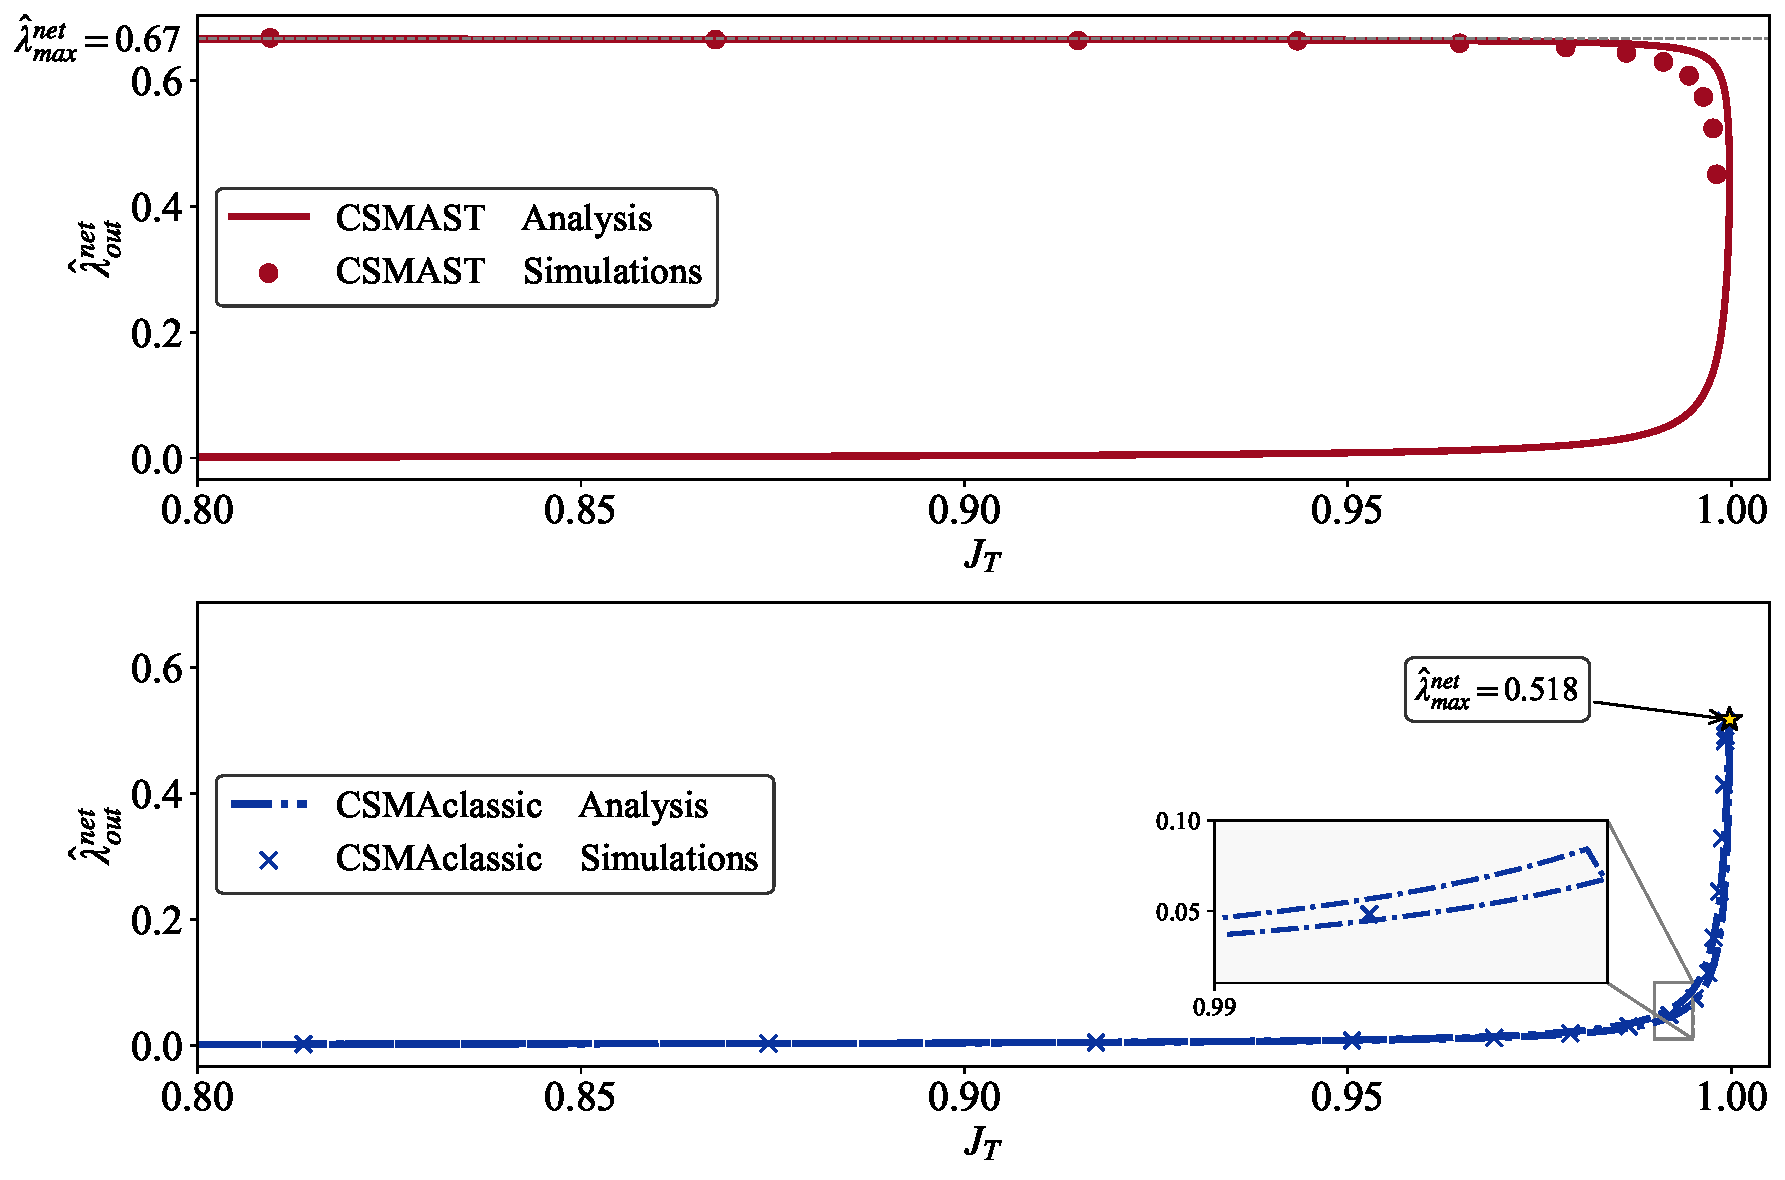
\includegraphics[width=0.7\textwidth]{figure/chap4/throughput_fairness_tradeoff.pdf}
	\caption{CSMAST 与经典 CSMA 机制的吞吐量-公平性轨迹对比（$n=100,\tau_S=5,\tau_F=3,\tau_I=1,T=10^6$）}
	\label{fig:comparison_classic}
\end{figure}

图~\ref{fig:csmast_jain_vs_t_multi_q} 进一步展示了不同接入概率 $q$ 下短期公平性 $J_T$ 随观测时间窗口 $T$ 的变化。实验参数设置为节点数 $n=100$、成功传输时长 $\tau_S=5$、碰撞时长 $\tau_F=3$、空闲时长 $\tau_I=1$。不同 $q$ 条件下理论曲线与仿真结果保持一致。结果表明，随着观测窗口增大，$J_T$ 整体上升并逐步趋于稳定，这与式 \ref{eq:jain_explicit} 中公平性随 $T$ 增大而改善的理论相符。可见，较短观测窗口内统计量更易受到连续忙期波动影响，节点间服务差异更明显；当观测窗口扩展后，碰撞重分配与多轮接入过程得到充分平均，短时不公平被逐步平滑。

\subsection{CSMAST 与 CSMA 机制的性能对比与分析}

图 \ref{fig:comparison_classic} 进一步展示了 CSMAST 与经典 CSMA 方案在吞吐量与公平性二维平面上的性能轨迹对比。对比实验采用统一参数设置：节点数 $n=100$、成功传输时长 $\tau_S=5$、碰撞时长 $\tau_F=3$、空闲时长 $\tau_I=1$，观测时长 $T=10^6$。经典 CSMA 的性能曲线基于附录\ref{app:classic_csma} 中推导的理论公式所绘制，保证两者是在完全相同的时隙结构参数 $x, y$ 以及统一分析框架下进行比较。通过遍历传输概率 $q$，可以得到两种方案在不同工作点下的性能包络。对比结果表明，在同等公平性水平下，CSMAST 的吞吐量高于经典 CSMA。具体而言，经典 CSMA 的最大理论吞吐量约为 0.518，而 CSMAST 可提升至 0.667，对应约 28.8\% 的吞吐量提升。

进一步分析可知，在低吞吐量区间（$\lambda^{net}_{out}<0.518$，对应较大 $q$）两种机制轨迹近乎重合。其原因是强竞争使信道在空闲与碰撞状态间高频切换，从而令两者的假期基本一致；此时性能差异主要由忙期 $\overline{B}$ 决定。随着 $q$ 减小，CSMAST 通过连续传输拉长 $\overline{B}$ 并提升吞吐量；随着 $q$ 增大，碰撞使忙期退化至近单包时长，机制行为趋近经典 CSMA。连续传输会在短时间尺度放大服务不对称现象并影响瞬时公平性，但其对假期的分布特性的影响有限，因此在长期统计意义下，两种机制的 Jain 指数保持接近。综上，CSMAST 可通过较小 $q$ 在可控公平代价下获得吞吐量增益。

\section{本章小结}

本章针对载波侦听接入网络的性能瓶颈，提出了基于连续传输的 CSMAST 机制。考虑到 CSMA 协议的状态时长异构性，本章引入吸收马尔可夫链理论，构建休假排队分析框架，成功推导了饱和状态下网络吞吐量与 Jain 公平性指数的闭式解。
理论与仿真分析表明，在一组相同配置条件下，CSMAST 相比传统 CSMA 实现了约 28.8\% 的吞吐量提升，同时还能保持较好的公平性。


        \newclearpage
        \chapter{基于监督学习的智能协议与参数联合选择方法}

\label{chapter5: ai_selector}
现代无线网络，尤其是物联网场景，业务需求呈现出显著的多样性与动态性。不同业务在接入密度、数据包长度及时延敏感度等方面差异明显，使得单一随机接入协议难以在复杂多变的网络条件下始终保持最优性能。传统基于固定协议与静态参数配置的设计，难以同时兼顾吞吐量、时延、公平性、信令开销多维性能指标，存在明显局限。
不同随机接入协议在吞吐性能、时延特性、信令开销方面表现各异。表~\ref{tab:protocol_comparison} 对 SA、SAST、CBA三种协议进行定性对比，可以看出，协议机制的增强虽可显著提升系统吞吐，但同时也可能带来更高的信令开销，进一步表明难以依靠单一协议适应所有场景。

\begin{table}[htbp]
\centering
\caption{不同随机接入协议的定性性能对比}
\label{tab:protocol_comparison}
% \renewcommand{\arraystretch}{1.2}
\begin{tabular}{c|c|c|c}
\hline
\textbf{协议} & \textbf{吞吐性能} & \textbf{时延特性} & \textbf{信令开销} \\
\hline
SA & 低 & 低 & 中 \\
\hline
SAST & 中 & 中 & 低 \\
\hline
CBA & 高 & 中-高 & 高 \\
\hline
\end{tabular}
\end{table}
因此，依据场景特征动态选择接入协议并联合优化其关键参数，是提升系统整体性能的有效途径。围绕这一需求，本章研究如何在多协议共存的统一框架下，根据业务流量状态智能决策最优协议及其参数配置。
针对此问题，本文提出一种面向动态业务场景的、基于监督学习的协议与参数联合选择方法，实现接入策略由静态向与数据驱动转变，从而在吞吐量、时延与公平性等多维性能之间取得更优平衡。

\section{问题建模与统一接入框架设计}
本节给出统一问题建模与接入框架。核心目标是在动态流量下实现协议与参数的联合自适应选择，以提升系统整体性能。
具体地，\ref{subsec:problem_formulation}小节给出联合优化问题建模，\ref{subsec:unified_input}小节构造统一输入特征，\ref{subsec:sim_mapping_utility}小节定义仿真映射与效用函数，\ref{subsec:equiv_constrained_opt}小节给出等价约束优化形式。


% 该统一框架的核心目标是将各类随机接入协议抽象为若干可调度、可配置的统计接入模式，并以网络的统计特征，尤其是业务流量的时序与分布属性，作为驱动信号，决策协议类型及其关键参数的自适应调整。通过将接入机制的设计从传统的协议逻辑层提升到统计建模与决策层，本框架为后续引入监督学习等数据驱动的方法提供了统一、可扩展的理论支撑与工程实现路径。

\subsection{问题建模}
\label{subsec:problem_formulation}

为便于后续章节统一叙述，这里首先对问题进行简要建模。对于任意网络场景，我们用统一输入向量 $\mathbf{X}_{\mathrm{in}}$ 表征其关键配置与状态特征，包括业务流量特征、网络规模以及可选接入协议的候选范围及协议参数等。
在给定 $\mathbf{X}_{\mathrm{in}}$ 后，我们通过统一仿真器或由监督学习方法构建的性能预测模型评估该配置下的系统性能。记该评估过程为一个映射 $S(\cdot)$，其输出为多维性能指标向量 $\mathbf{y}=S\big(\mathbf{X}_{\mathrm{in}}\big)$。为便于跨场景与跨协议比较性能，引入归一化算子 $\mathrm{norm}(\cdot)$，得到归一化后的指标向量 $\tilde{\mathbf{y}}=\mathrm{norm}(\mathbf{y})$。在此基础上，用综合效用函数 $U(\cdot)$ 将 $\tilde{\mathbf{y}}$ 映射为单一的效用得分。

在上述定义下，我们希望从若干候选接入协议及其允许的参数配置中，选出使综合效用最大的那一组。该联合选择问题可形式化表述为：
\begin{equation}
\label{eq:chap5_overview}
\mathbf{x}_{\mathrm{proto}}^*
=\arg\max_{\mathbf{x}_{\mathrm{proto}}}
U\!\left(\mathrm{norm}\!\left(S\big(\mathbf{X}_{\mathrm{in}}\big)\right)\right),
\end{equation}
其中决策变量为统一参数向量 $\mathbf{x}_{\mathrm{proto}}$，其首个分量为协议类型标识符，其余分量为对应协议参数。记 $\mathbf{x}_{\mathrm{proto}} = [a, \mathbf{x}_p]$，其中 $a \in \mathcal{P}$ 表示从候选集合中选取的协议类型，$\mathbf{x}_p \in \mathcal{X}_p$ 为该协议的参数向量，$\mathcal{X}_a$ 为协议 $a$ 的合法参数空间。图~\ref{fig:chap5_framework} 给出了统一接入框架及协议选择流程的示意，后续内容将围绕式~\eqref{eq:chap5_overview} 分别展开统一输入构造、性能指标与效用定义以及数据驱动决策方法的设计。
\begin{figure}[t]
\centering
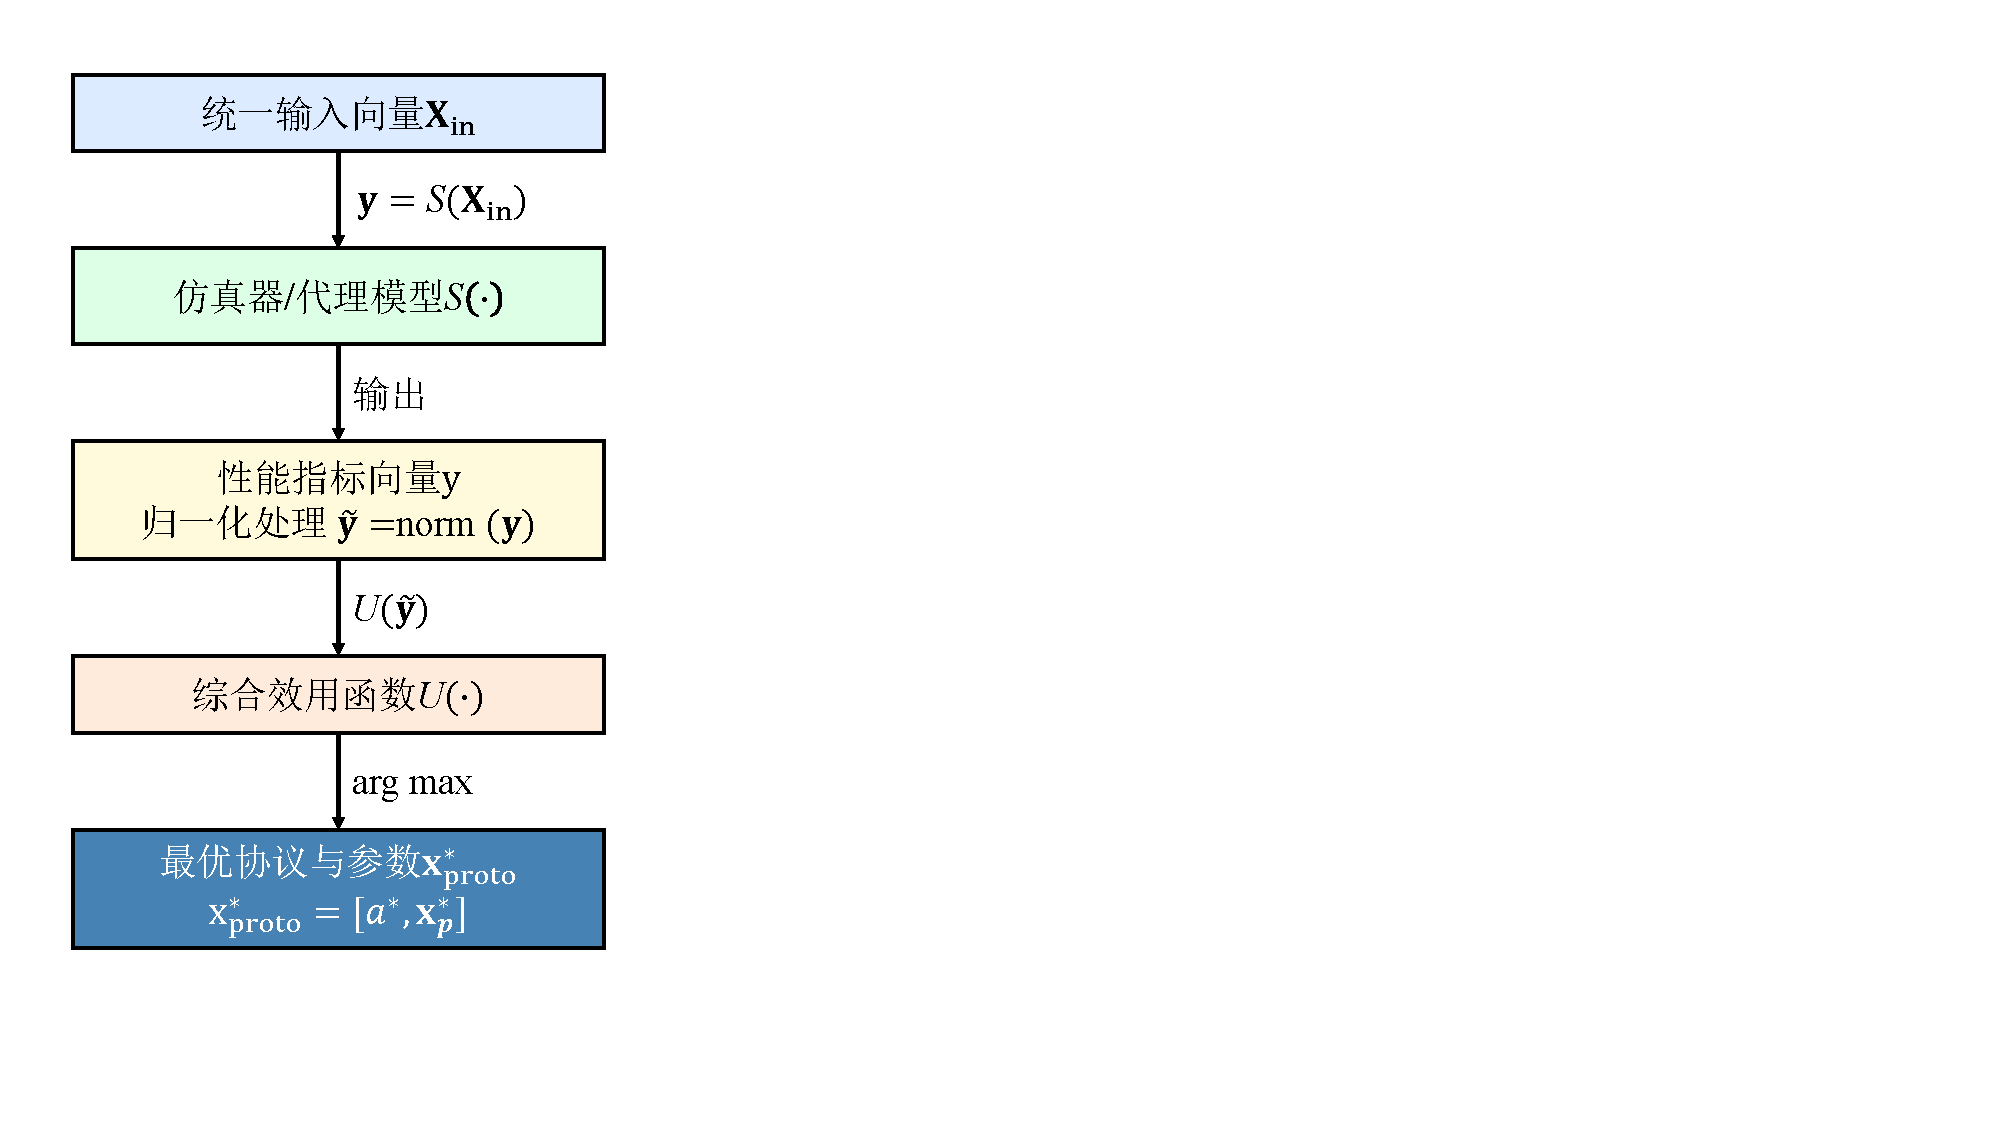
\includegraphics[width=0.95\textwidth]{figure/chap5/model1.pdf}
\caption{统一接入框架与协议选择流程}
\label{fig:chap5_framework}
\end{figure}


\subsection{输入特征标准化与统一接口}
\label{subsec:unified_input}
为实现式~\eqref{eq:chap5_overview} 所需的输入表达，本小节给出统一输入 $\mathbf{X}_{\mathrm{in}}$ 的可实现构造方法。本文将特征划分为三类：通用网络参数 $\mathbf{x}_{\mathrm{common}}$，业务流量特征参数 $\mathbf{x}_{\text{traffic}}$，以及协议专属参数 $\mathbf{x}_{\mathrm{proto}}$ 及其有效性掩码 $\mathbf{m}$。

对于通用网络参数 $\mathbf{x}_{\mathrm{common}}$，将其定义为包含网络规模与仿真配置的向量：
$\mathbf{x}_{\mathrm{common}} = [n,\ T]$,
其中 $n \in \mathbb{N}^+$ 表示网络节点总数，$T \in \mathbb{N}^+$ 表示仿真或观测的时隙总数。上述参数既用于构建仿真场景，也作为后续学习模型的输入特征，共同刻画系统的整体运行条件。

对于业务流量特征 $\mathbf{x}_{\text{traffic}}$，为准确刻画业务到达的多尺度时空统计特性，本文从网络层与节点层两个层级，分别提取负载强度、突发性与周期性三类特征。具体地，定义五维流量特征向量 $\mathbf{x}_{\text{traffic}} = [\hat{\lambda},\ \mathrm{BI}_{\mathrm{net}},\ \mathrm{BI}_{\mathrm{node}},\ \Psi_{\mathrm{net}},\ \Psi_{\mathrm{node}}]$。

设到达矩阵 $\mathbf{A} \in \{0,1\}^{n \times T}$，其中 $A_{i,t}$ 表示节点 $i$ 在时隙 $t$ 是否有包到达。记网络聚合到达序列为 $X(t) = \sum_{i=1}^{n} A_{i,t}$，节点 $i$ 的到达时刻集合为 $\mathcal{T}_i = \{t : A_{i,t} = 1\}$，到达间隔序列为 $\{\Delta t_i^{(k)}\}$，其中 $\Delta t_i^{(k)}$ 为节点 $i$ 第 $k$ 次与第 $k+1$ 次到达的时间间隔。基于此，五维特征定义如下：

\begin{table}[htbp]
\centering
\caption{业务流量特征参数$\mathbf{x}_{\text{traffic}}$的定义与表征含义}
\label{tab:traffic_feature_def}
\renewcommand{\arraystretch}{1.25}
\small
\begin{tabular}{p{2.6cm}|p{1.4cm}|p{6.2cm}|p{4.2cm}}
\toprule
\textbf{名称} & \textbf{变量} & \textbf{计算公式} & \textbf{表征含义} \\
\midrule

归一化网络平均到达率 
& $\hat{\lambda}$ 
& $\hat{\lambda}=\frac{1}{nT}\!\sum_{t=1}^{T}\sum_{i=1}^{n}A_{i,t}$ 
& 表征系统整体流量强度，反映平均活跃节点占比 \\
\hline

网络突发度指标 
& $\mathrm{BI}_{\mathrm{net}}$ 
& $\mathrm{BI}_{\mathrm{net}}
=\frac{\mathrm{ID}_{\mathrm{net}}-1}{\mathrm{ID}_{\mathrm{net}}+1},\;
\mathrm{ID}_{\mathrm{net}}
=\frac{\mathrm{Var}(X(t))}{\mathbb{E}[X(t)]}$ 
& 刻画网络聚合流量的突发性 \\
\hline

节点突发度指标 
& $\mathrm{BI}_{\mathrm{node}}$ 
& $\mathrm{BI}_{\mathrm{node}}
=\frac{\overline{\mathrm{CV}}-1}{\overline{\mathrm{CV}}+1},\;
\overline{\mathrm{CV}}
=\frac{1}{n}\sum_{i=1}^{n}
\frac{\sqrt{\mathrm{Var}(\Delta t_i)}}{\mathbb{E}[\Delta t_i]}$ 
& 刻画单节点到达间隔的突发性 \\
\hline

网络周期性强度 
& $\Psi_{\mathrm{net}}$ 
& $\Psi_{\mathrm{net}}
=\max_{1\le\tau\le\tau_{\max}}
\frac{R(\tau)}{R(0)},
R(\tau)
=\frac{1}{T}\sum_{t=1}^{T-\tau}
\tilde{X}(t)\tilde{X}(t+\tau)$ 
& 网络聚合到达序列的周期性强度 \\
\hline

节点周期性强度 
& $\Psi_{\mathrm{node}}$ 
& $\Psi_{\mathrm{node}}
=\frac{1}{n}\sum_{i=1}^{n}
\max\!\left(0,1-
\frac{\mathrm{Var}(\Delta t_i)}
{(\mathbb{E}[\Delta t_i])^{2}}\right)$ 
& 单节点到达间隔的周期性强度 \\
\bottomrule

\end{tabular}
\end{table}

对于协议专属参数 $\mathbf{x}_{\mathrm{proto}}$，本文采用统一参数超集与掩码的表示方案，以在多协议共存场景下建立统一的输入接口。设候选接入协议集合为 $\mathcal{P} = \{a_1, a_2,  a_3\}$，包括 SA、SAST、CBA协议。每一种协议 $a \in \mathcal{P}$ 对应一组可调参数集合 $\mathcal{X}_p$。
为消除因协议参数维度不一致而产生的维度非对齐问题，本文将候选协议集合中所有参数的并集统一放入一个高维参数向量 $\mathbf{x}_{\mathrm{proto}} \in \mathbb{R}^{d_{\max}}$，其中 $d_{\max} = 1 + \max_{a  \in \mathcal{P}} |\mathcal{X}_p|$ 为统一向量维度，包含协议标识符及所有协议参数的超集。该向量的第一个分量为协议类型标识符 $a \in \mathcal{P}$，其余分量包含接入概率 $q$、连续传输长度 $M$等所有可能的协议参数；当某一协议不涉及其中部分参数时，对应维度仍保留作为占位符。统一参数向量的完整形式为：
$\mathbf{x}_{\mathrm{proto}} = [a, q,\ M, \ldots]$, 
其中省略号对应除列示参数外的其余占位分量。

为严格刻画占位参数在当前协议下的有效性，我们引入与 $\mathbf{x}_{\mathrm{proto}}$ 同维的二值掩码向量 $\mathbf{m} \in \{0,1\}^{d_{\max}}$。在预处理与模型输入阶段，对应掩码为零的参数分量通过元素级乘积 $\mathbf{x}_{\mathrm{proto}} \odot \mathbf{m}$ 被统一置零或屏蔽，从而在保留统一维度表示的同时，防止无效参数对后续学习与优化过程造成干扰。输入特征与性能指标的摘要见表~\ref{tab:input_features}。
完整标准化输入向量表示为
\begin{equation}
\mathbf{X}_{\mathrm{in}} = \big[\mathbf{x}_{\text{traffic}},\ \mathbf{x}_{\mathrm{common}},\ \mathbf{x}_{\mathrm{proto}},\ \mathbf{m}\big].
\end{equation}


\begin{table}[t]
	\centering
	\caption{标准化输入与性能指标摘要}
	\label{tab:input_features}
	\renewcommand{\arraystretch}{1.2}
	\begin{tabular}{@{}l | l | p{9cm}@{}}
	\toprule
		特征组 & 符号 & 含义 / 备注 \\
		\midrule
		$\mathbf{x}_{\text{traffic}}$ & $\hat{\lambda}$ & 归一化网络平均到达率，范围 $[0, 1]$。\\
		& $\mathrm{BI}_{\mathrm{net}}$ & 网络突发度指标，范围 $(-1,1)$。\\
		& $\mathrm{BI}_{\mathrm{node}}$ & 节点突发度指标，范围 $(-1,1)$。\\
		& $\Psi_{\mathrm{net}}$ & 网络周期性强度，范围 $[0,1]$。\\
		& $\Psi_{\mathrm{node}}$ & 节点周期性强度，范围 $[0,1]$。\\
		\midrule
		$\mathbf{x}_{\mathrm{common}}$ & $n$ & 节点数量。\\
		& $T$ & 时隙数量。\\
		\midrule
		$\mathbf{x}_{\mathrm{proto}}$ & $a$ & 协议类型标识，$a\in\mathcal{P}$（向量第一个分量）。\\
		& $q$ & 接入概率。\\
		& $M$ & 连续传输长度。\\
		\midrule
		$\mathbf{m}$ & $m_k$ & 有效性掩码：$m_k=1$ 若第 $k$ 个协议参数在当前协议下有效，否则为 $0$。\\
		\midrule
		$\mathbf{y}$ & $\lambda_{\mathrm{out}}$ & 吞吐量。\\
		& $D$ & 平均时延。\\
		& $J_T$ & 公平性。采用 Jain 指数并做归一化。\\
		& $S$ & 信令开销 \\
		\bottomrule
	\end{tabular}
\end{table}

\subsection{统一仿真映射与效用构造}
\label{subsec:sim_mapping_utility}

在统一输入接口 $\mathbf{X}_{\mathrm{in}}$ 确定后，需要进一步给出从输入到性能度量的可复现映射。为此，本文构建统一的离散事件仿真映射$S(\cdot)$，输入为统一输入向量 $\mathbf{X}_{\mathrm{in}}$，仿真器据此生成对应网络场景并执行随机接入过程，最终输出性能—资源指标向量
\begin{equation}
	\mathbf{y}=S\!\left(\mathbf{X}_{\mathrm{in}}\right)
	=\big[\lambda_{\mathrm{out}},\ D,\ J_T,\ S,\big],
\end{equation}
其中 $\lambda_{\mathrm{out}}$ 表示系统吞吐量，$D$ 表示平均数据包时延，$J_T$ 表示公平性（采用 Jain 指数刻画），$S$ 表示信令开销。上述指标集合兼顾业务性能与代价，便于在多协议、多参数配置下进行统一评估与对比。
为消除不同指标量纲与数值尺度差异对比较与决策造成的影响，并保证跨协议评估的一致性，本文在同一对比组内对各维指标采用最小最大归一化，并将所有指标统一转换为效用型指标。记第 $k$ 个指标 $y_k$ 在对比组内的取值范围为 $[y_k^{\min}, y_k^{\max}]$，则归一化后的指标 $\tilde{y}_k$ 定义为
\begin{equation}
	\tilde{y}_k =
	\begin{cases}
	\dfrac{y_k-y_k^{\min}}{y_k^{\max}-y_k^{\min}}, & y_k \ \text{为效用型指标},\\[10pt]
	1-\dfrac{y_k-y_k^{\min}}{y_k^{\max}-y_k^{\min}}, & y_k \ \text{为成本型指标},
	\end{cases}
\end{equation}
其中效用型指标是指数值增大表示性能提升的指标，如吞吐量 $\lambda_{\mathrm{out}}$ 和公平性 $J_T$；成本型指标是指数值减小表示性能改善的指标，如时延 $D$ 与信令开销 $S$。该归一化方法将所有指标映射至 $[0,1]$ 区间，并保证归一化后的指标均满足数值越大性能越优的单调关系。由此得到归一化指标向量
\begin{equation}
	\tilde{\mathbf{y}}=\mathrm{norm}(\mathbf{y})
	=\big[\tilde{\lambda}_{\mathrm{out}},\ \tilde{D},\ \tilde{J}_T,\ \tilde{S}\big].
\end{equation}

在此基础上，为将多维指标映射为单一可优化目标，本文采用加权线性效用函数
\begin{equation}
	U\big(\tilde{\mathbf{y}}\big)=
	w_{\lambda}\tilde{\lambda}_{\mathrm{out}}
	+w_{D}\tilde{D}
	+w_{J}\tilde{J}_T
	+w_{S}\tilde{S},
\end{equation}
其中 $w_i\ge 0$ 且 $\sum_i w_i=1$。权重向量 $\{w_i\}$ 用于表征业务对吞吐、时延、公平性以及信令开销的偏好，可依据应用需求设定；同时，可通过改变权重进行敏感性分析，以检验联合选择结论的稳健性。

\subsection{等价资源约束下的联合优化问题}
\label{subsec:equiv_constrained_opt}
为便于后续性能预测模型训练与快速优化算法中目标计算、约束检查与可行域投影的统一实现，本节将式~\eqref{eq:chap5_overview} 所述问题改写为标准约束优化形式。该表述与原问题在决策变量、优化目标及约束条件上完全等价，区别仅在于将隐式关系显式展开，以适配标准优化求解器的输入要求。

优化问题的标准形式表述如下：
\begin{equation}\label{eq:chap5_constrained}
	\begin{aligned}
		\max_{\,\mathbf{x}_{\mathrm{proto}}\in\mathcal{X}} \quad 
		& U\big( \tilde{\mathbf{y}} \big) \\[6pt]
		\text{s.t.}\quad
		& \mathbf{X}_{\mathrm{in}}=\big[\mathbf{x}_{\text{traffic}},\ \mathbf{x}_{\mathrm{common}},\ \mathbf{x}_{\mathrm{proto}},\ \mathbf{m}\big],\\[3pt]
		& \tilde{\mathbf{y}} = \mathrm{norm}\!\left(\mathbf{y}\right),\ \mathbf{y} = S\!\left( \mathbf{X}_{\mathrm{in}} \right), \\[4pt]
		& S\big(\mathbf{x}_{\mathrm{proto}}\big) \le S_{\max}.
	\end{aligned}
\end{equation}
式~\eqref{eq:chap5_constrained} 的决策变量为统一参数向量 $\mathbf{x}_{\mathrm{proto}}$，其第一个分量 $\mathbf{x}_{\mathrm{proto}}[1]$ 为协议标识符，其余分量为各协议参数。决策变量需满足所选协议的合法参数空间约束，通过掩码 $\mathbf{m}$ 界定有效参数维度。第一行约束显式构建统一输入向量，第二行约束定义从输入到归一化性能指标的映射关系。第三行约束限定信令开销不超过系统资源阈值 $S_{\max}$。
可以看到，该优化问题的解为满足全部约束的最优统一参数向量 $\mathbf{x}_{\mathrm{proto}}^*$，其中包含了最优协议类型及其对应参数。


% =========================================================
% 第 5.2 节：仿真数据生成与性能分析
% =========================================================

\section{基于离散事件仿真的接入协议数据集构建与仿真结果分析}
\label{sec:simulation_data}

为训练能够准确预测不同协议配置下网络性能的模型，需要构建高质量的训练数据集。本节首先阐述参数空间的采样策略，随后在\ref{subsec:unified_simulator}小节介绍统一仿真器 $S(\cdot)$ 的设计与实现，接着详细说明基于仿真器的数据集生成流程，最后通过可视化分析展示不同协议在典型场景下的性能差异，为后续性能预测模型的构建提供数据基础与性能基准。

\subsection{两阶段参数空间采样策略}
\label{subsec:grid_sampling}

训练数据质量取决于参数空间覆盖与关键区域分辨率。为兼顾两者，本文在混合空间 $\{\mathbf{x}_{\text{traffic}},\mathbf{x}_{\mathrm{proto}}\}$ 上采用“两阶段采样”策略：第一阶段做全局粗采样，第二阶段做峰值与转折区细采样。采样维度分为流量强度 $\hat{\lambda}$、流量形态、协议参数三类，其中流量形态在两个阶段均固定为三类场景并保持一致遍历，以保证跨协议、跨阶段结果可比。图~\ref{fig:dataset_sampling_strategy} 给出流程示意。

\begin{figure}[t]
	\centering
	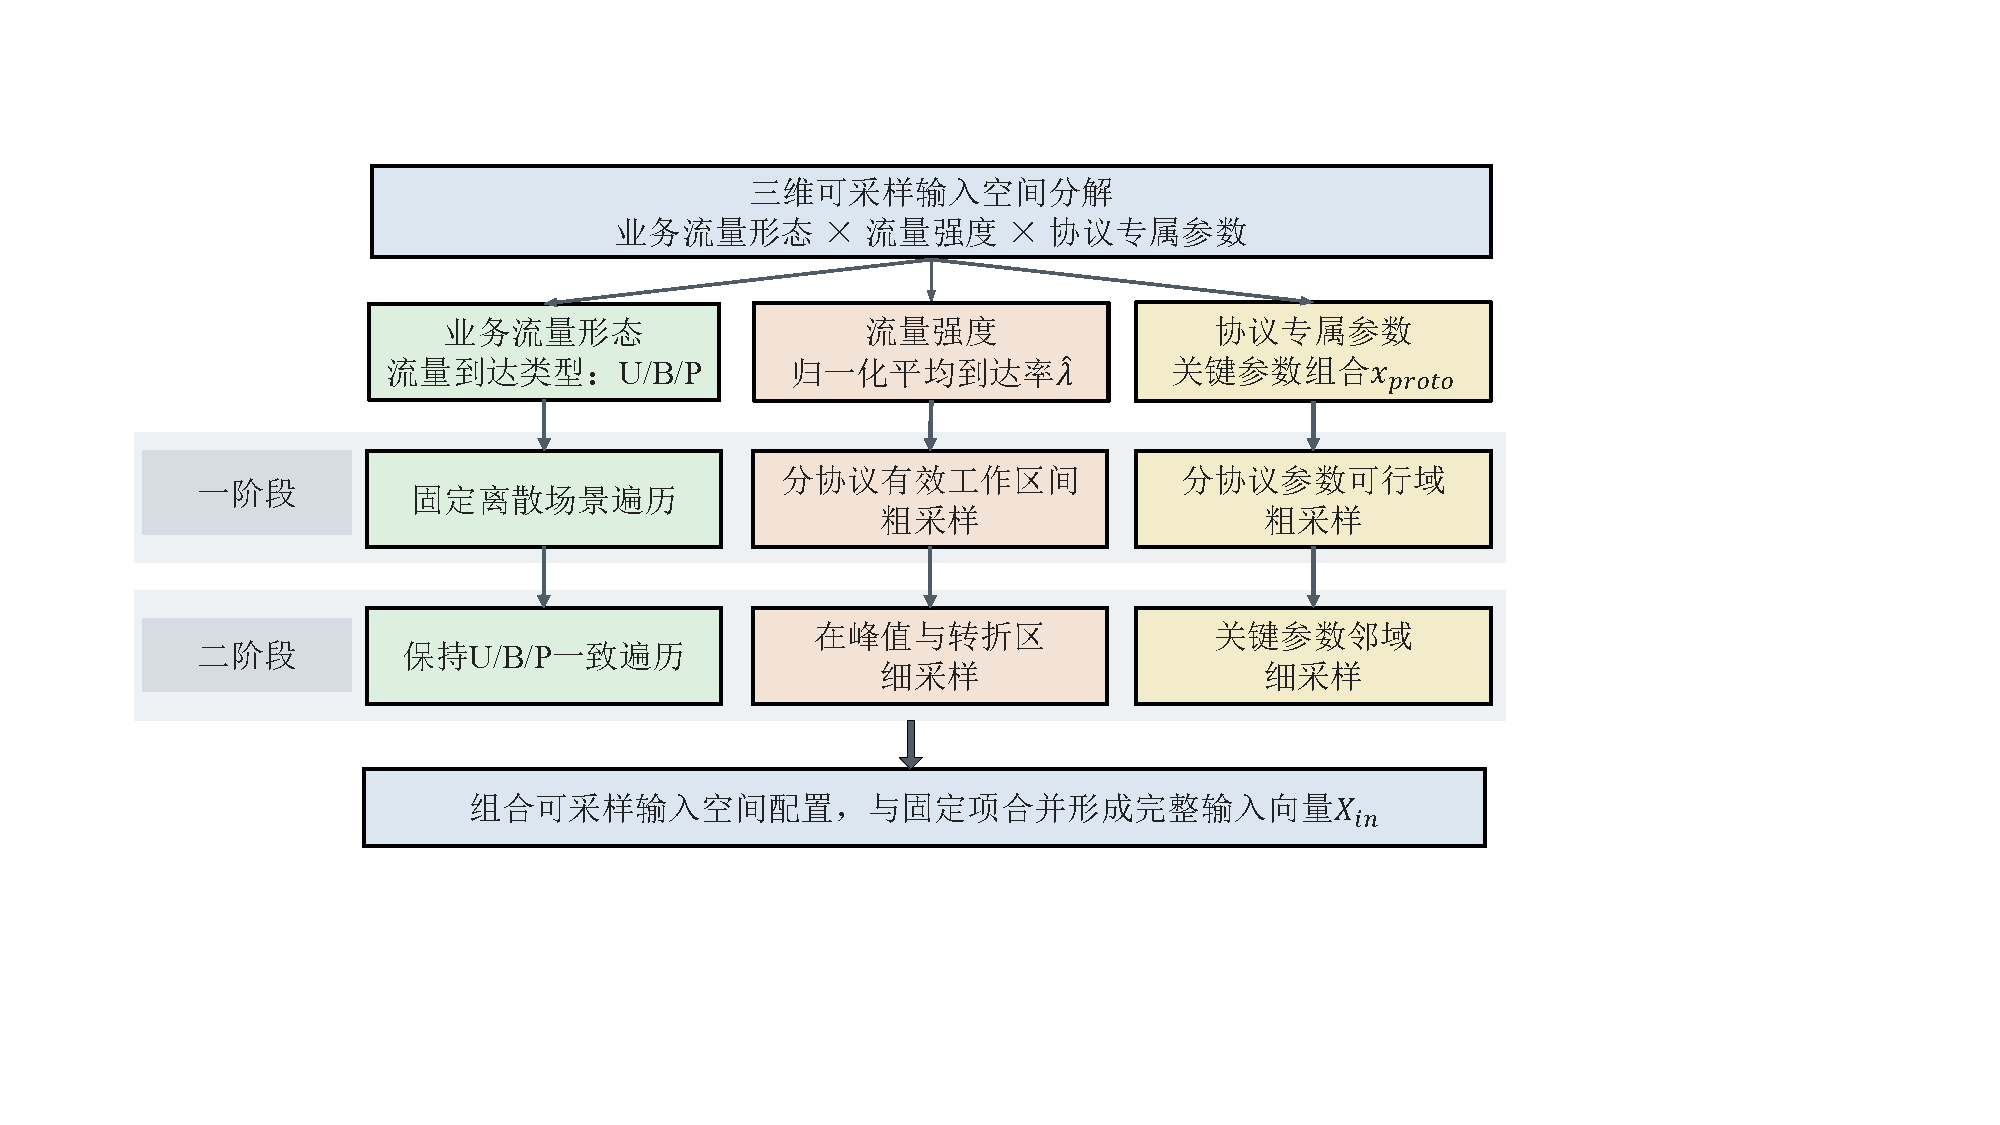
\includegraphics[width=0.99\textwidth]{figure/chap5/数据集采样策略.pdf}
	\caption{两阶段参数空间采样策略流程图}
	\label{fig:dataset_sampling_strategy}
\end{figure}
流量形态维度采用三类离散场景：均匀到达（U）、突发到达（B）、周期到达（P）。在第一阶段与第二阶段中，任一 $\hat{\lambda}$ 与任一协议参数组合都必须在 U/B/P 三类流量下分别仿真一次，确保每阶段数据集都包含三类流量样本。

% 其流量特征为 $\mathrm{BI}_{\mathrm{net}} \approx 0$ 且 $\Psi_{\mathrm{net}} \approx 0$，对应近似泊松到达过程。
% 其流量特征为 $\mathrm{BI}_{\mathrm{net}} \in [0.3, 0.7]$ 且 $\Psi_{\mathrm{net}} \in [0, 0.2]$，表征中等至强突发性。
% 其流量特征为 $\mathrm{BI}_{\mathrm{net}} \in [-0.5, -0.2]$ 且 $\Psi_{\mathrm{net}} \in [0.6, 0.9]$，体现规则周期结构。

第一阶段为粗粒度均匀采样，其目标是在较低计算成本下获取各协议性能曲线的全局轮廓。核心原则是按协议有效工作区间设置差异化 $\hat{\lambda}$ 采样范围，而非统一范围。
具体而言，SA 的理论最大吞吐约为 $1/e\approx0.368$，因此其采样点应主要落在 $[0,1/e]$；仅保留少量 $>1/e$ 的样本点用于刻画饱和边界。SAST 的有效高吞吐区通常延伸至约 0.5，采样上限应相应提高。CBA 在较高负载下仍可能保持较好吞吐，其上限可进一步放宽，但仍以可工作区间为准，避免无效超载样本。
对于每个粗采样点，均在 U/B/P 三类流量下生成样本，从而可在相同平均到达率下直接比较不同流量形态对协议性能的影响。
协议参数亦采用针对各协议的专属粗采样：连续参数（如 $q$）作稀疏均匀取点，离散参数（如 $M$）遍历典型可行值，二者的笛卡尔积构成第一阶段配置集合。综上，第一阶段样本由协议类型、流量强度粗网格、协议参数粗网格与三类流量形态共同组成。基于该阶段结果，可进一步定位各协议在不同流量形态下的峰值区与性能转折区。

第二阶段为峰值及转折区域细采样，从而进一步提高采样分辨率。具体实现方法为：根据第一阶段结果，为每种协议在每类流量形态下确定峰值区间与转折区间，在该区间内以更小步长对 $q$ 进行局部加密采样，以提升最优工作点邻域的采样分辨率。第二阶段的样本量根据各协议关键区间的宽度自适应确定。
最终将两阶段样本合并形成训练集：第一阶段保证全局覆盖，第二阶段强化关键区域。与全空间均匀细采样相比，该策略在控制样本规模的同时提高了最优工作点附近的建模精度。

% 为便于后续统一补充实验数据，表~\ref{tab:two_stage_sampling_template} 给出两阶段采样配置总表模板。

% \begin{table}[htbp]
% \centering
% \caption{两阶段采样配置总表（模板，待补充）}
% \label{tab:two_stage_sampling_template}
% \renewcommand{\arraystretch}{1.2}
% \setlength{\tabcolsep}{3pt}
% \small
% \begin{tabular}{p{0.9cm} p{1.0cm} p{1.3cm} p{2.2cm} p{1.0cm} p{3.2cm} p{3.0cm}}
% \toprule
% 协议 & 阶段 & 流量形态 & $\hat{\lambda}$采样区间 & 步长 & 协议参数采样设置 & 样本统计（单形态/三形态/有效） \\
% \midrule
% SA & 粗采样 & U/B/P & [\ ,\ ] & [\ ] & $q:\,$[\ ] & [\ ] / [\ ] / [\ ] \\
% SA & 细采样 & U/B/P & [\ ,\ ] & [\ ] & $q:\,$[\ ] & [\ ] / [\ ] / [\ ] \\
% SAST & 粗采样 & U/B/P & [\ ,\ ] & [\ ] & $q:\,$[\ ] & [\ ] / [\ ] / [\ ] \\
% SAST & 细采样 & U/B/P & [\ ,\ ] & [\ ] & $q:\,$[\ ] & [\ ] / [\ ] / [\ ] \\
% CBA & 粗采样 & U/B/P & [\ ,\ ] & [\ ] & $q:\,$[\ ], $M:\,$[\ ] & [\ ] / [\ ] / [\ ] \\
% CBA & 细采样 & U/B/P & [\ ,\ ] & [\ ] & $q:\,$[\ ], $M:\,$[\ ] & [\ ] / [\ ] / [\ ] \\
% \midrule
% \multicolumn{6}{r}{总计} & [\ ] / [\ ] / [\ ] \\
% \bottomrule
% \end{tabular}
% \end{table}



\subsection{统一仿真器的设计与实现}
\label{subsec:unified_simulator}

统一仿真器 $S(\cdot)$ 是连接输入配置与性能指标的核心映射模块，其设计需同时满足多协议支持、精确性与可扩展性要求。本文基于离散事件仿真框架采用模块化设计实现该仿真器，通过各模块的协调完成对三种随机接入协议的统一建模与性能评估。
统一仿真器采用分层模块化架构，包含以下核心组件：

\begin{itemize}[leftmargin=*]
	\item \textbf{配置解析模块}：解析统一输入向量 $\mathbf{X}_{\mathrm{in}}$，提取网络参数 $\mathbf{x}_{\text{common}}$、流量特征向量 $\mathbf{x}_{\text{traffic}}$ 以及协议专属参数向量 $\mathbf{x}_{\mathrm{proto}}$。其中 $\mathbf{x}_{\text{traffic}}$ 的可配置项为归一化平均到达率 $\hat{\lambda}$。此外，还需单独指定流量类型标识 $\text{traffic\_type}$ 以确定流量生成模型。

	\item \textbf{流量生成与特征提取模块}：依据流量类型标识 $\text{traffic\_type}$ 选择相应的到达过程模型，即均匀到达采用泊松过程、突发到达采用马尔可夫调制泊松过程、周期到达采用确定性周期同步过程，各类型模型的内部生成参数均预先设定。在给定归一化平均到达率 $\hat{\lambda}$ 下，为各节点按时隙生成到达包序列。由于生成参数固定，所得流量序列仅覆盖有限组预定义的突发强度与周期强度，从而保证不同实验配置间的可复现性。在此基础上，基于生成的到达包序列计算并输出 $\mathbf{x}_{\text{traffic}}$ 中除 $\hat{\lambda}$ 外的特征指标 $\mathrm{BI}_{\mathrm{net}}$、$\mathrm{BI}_{\mathrm{node}}$、$\Psi_{\mathrm{net}}$ 与 $\Psi_{\mathrm{node}}$。

	\item \textbf{协议执行与仿真模块}：协议策略由协议专属参数向量 $\mathbf{x}_{\mathrm{proto}}$ 参数化，其首个分量为协议类型标识 $a$，其余分量为对应协议的参数配置。仿真器在运行前根据协议标识 $a$ 加载相应的协议执行引擎，并在每个时隙依据参数策略完成发送决策与队列状态更新，同时与信道仿真子模块协同完成并行发送的冲突检测。各协议的核心接入机制封装如下：
	\begin{itemize}[leftmargin=*, itemsep=0.2em]
		\item \textbf{SA}：时隙Aloha协议，节点有数据包时以固定接入概率 $q$ 尝试发送。
		\item \textbf{SAST}：连续传输时隙Aloha协议，当上一时隙发送成功时接入概率置1并连续传输，否则恢复以概率 $q$ 随机接入。
		\item \textbf{CBA}：基于连接的Aloha协议，当节点缓存队列中数据包数量不小于 $M$ 时，以概率 $q$ 尝试建立连接，连接建立成功后无竞争地连续发送 $M$ 个数据包。
	\end{itemize}

	\item \textbf{性能统计模块}：实时记录成功发送包数、累计时延、各节点吞吐、信令开销等统计量，在仿真完成后计算最终的吞吐量 $\lambda_{\mathrm{out}}$、平均时延 $D$、公平性指数 $J_T$、信令开销 $S$。
\end{itemize}

上述模块通过统一接口在离散事件仿真框架下协同运行，从而实现对多协议、多参数配置的统一评估。仿真器的整体执行流程遵循初始化、时隙迭代与结果汇总三个阶段，如图~\ref{fig:unified_simulator_main} 所示。
\begin{figure}[t]
\centering
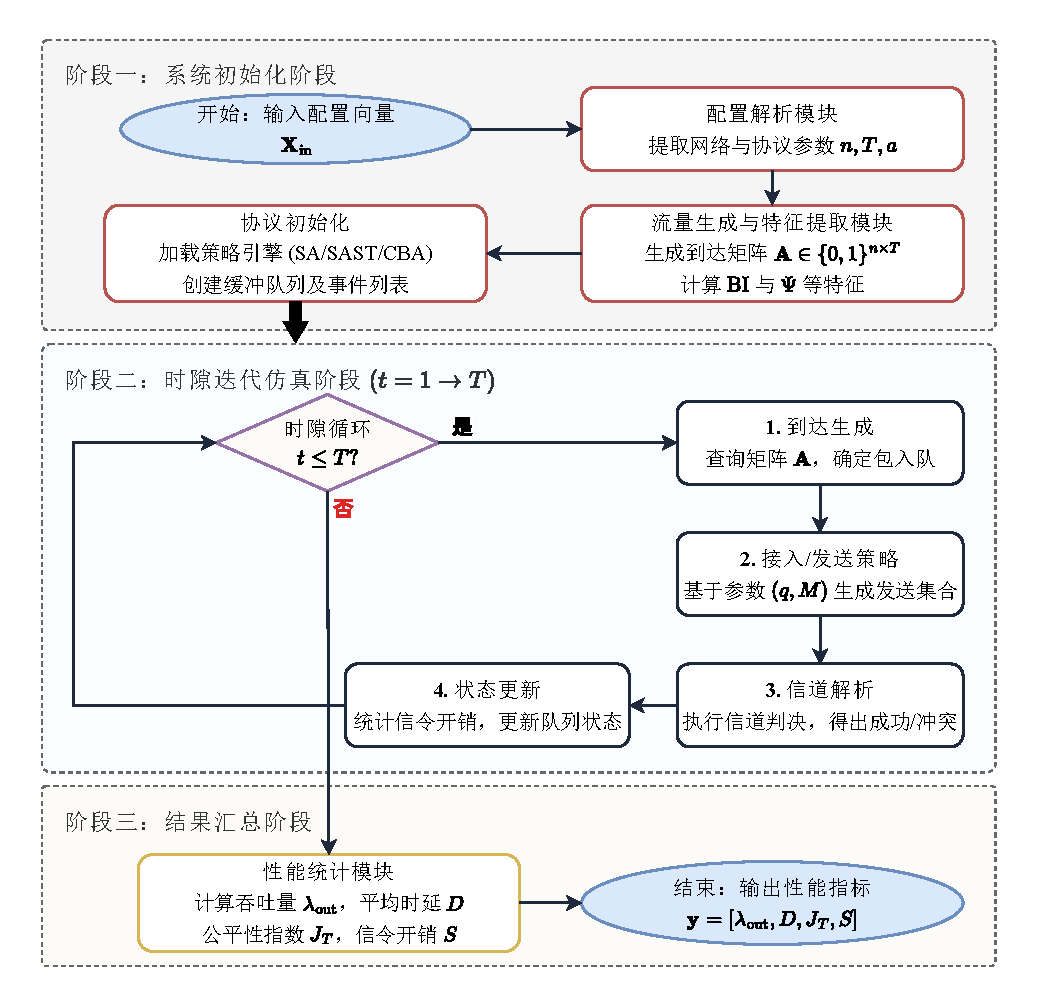
\includegraphics[width=0.95\textwidth]{figure/chap5/仿真器实现流程框图.pdf}
\caption{统一仿真器设计与实现流程图}
\label{fig:unified_simulator_main}
\end{figure}



% \begin{algorithm}[htbp]
% 	\caption{统一仿真器执行流程}
% 	\label{alg:unified_simulator_main}
% 	\KwIn{配置参数 $\mathbf{X}_{\text{in}} = (\mathbf{x}_{\mathrm{common}}, \mathbf{x}_{\text{traffic}}, \mathbf{x}_{\mathrm{proto}}, \mathbf{m})$, \text{traffic\_type} }
% 	\KwOut{性能指标 $\mathbf{y} = [\lambda_{\mathrm{out}}, D, J_T, S]$}
	
% 	配置解析模块：$n, T, \text{traffic\_type}, \hat{\lambda}, \mathbf{x}_{\mathrm{proto}} \leftarrow \text{Parse}(\mathbf{X}_{\text{in}})$\\
% 	协议标识提取：$a \leftarrow \mathbf{x}_{\mathrm{proto}}[1]$\\
% 	系统初始化：创建 $n$ 个节点的缓冲队列、信道状态记录、事件队列\\
% 	流量生成与特征提取：基于 $\text{traffic\_type}$ 和归一化网络平均到达率 $\hat{\lambda}$ 选择到达过程（参数预设），生成到达矩阵 $\mathbf{A}\in\{0,1\}^{n\times T}$，并计算更新 $\mathrm{BI}_{\mathrm{net}}$、$\mathrm{BI}_{\mathrm{node}}$、$\Psi_{\mathrm{net}}$、$\Psi_{\mathrm{node}}$\\
% 	加载协议引擎以及参数：根据$a$加载协议执行引擎，根据$\mathbf{x}_{\mathrm{proto}}$加载协议策略\\

% 	性能统计初始化：$\text{success\_counter} \leftarrow 0, \text{delay\_counter} \leftarrow 0, \text{signaling\_cost} \leftarrow 0$\\
% 	\For{$t = 1$ \textbf{to} $T$}{
% 		1. 到达生成：由到达矩阵$\mathbf{A}\in\{0,1\}^{n\times T}$确定各节点的包入队情况\;
		
% 		2. 接入/发送策略：根据协议规则与协议参数生成发送集合\;
		
% 		3. 信道解析：执行信道判决，得到并行发送导致的成功/冲突结果\;
		
% 		4. 统计信令开销：根据协议机制统计本时隙信令相关操作（如连接建立、预约、反馈等）\;
		
% 		5. 根据成功结果更新队列/协议内部状态，并更新统计量\;
% 	}
% 	计算吞吐量：$\lambda_{\mathrm{out}} \leftarrow \text{success\_counter} / T$\\
% 	计算平均时延：$D \leftarrow \text{sum\_delay} / \text{success\_counter}$\\
% 	计算公平性指数：$J_T \leftarrow \text{Jain}(\text{node\_throughputs})$\\
% 	计算信令开销：$S \leftarrow \text{sum\_signaling\_cost} / T$\\
% 	组织输出：$\mathbf{y} \leftarrow [\lambda_{\mathrm{out}}, D, J_T, S]$\\
% 	\Return $\mathbf{y}$
% \end{algorithm}

% 通过上述设计，统一仿真器能够高效、准确地评估不同协议配置下的网络性能，为数据集构建提供可靠的性能标签。仿真配置与数据统计信息在表~\ref{tab:dataset_summary}中统一汇总。

\subsection{数据集构建与预处理}
\label{subsec:dataset_construction}

基于两阶段采样策略与统一仿真器，本文构建了覆盖三种协议、多种流量强度与参数配置的综合性能数据集。数据集构建过程如下：
\begin{enumerate}[leftmargin=*]
	\item \textbf{采样执行}：针对候选协议集合 $\mathcal{P} = \{\text{SA, SAST, CBA}\}$，依照前述网格搜索策略生成参数组合。各采样变量与仿真器关键参数一一对应，主要参数与统计结果统一汇总于表~\ref{tab:dataset_summary}。以SA协议为例，主要参数包括归一化网络平均到达率$\hat{\lambda}$和接入概率 $q$，分别在设定区间内均匀采样，最终形成多组参数配置。

	\item \textbf{仿真执行}：对每组参数配置，调用统一仿真器开展仿真实验。仿真器在固定网络规模与仿真时隙数下运行并输出各项性能指标。为降低随机性影响，每组配置重复进行多次独立实验，以各项性能指标的均值作为该配置的性能标签。

	\item \textbf{数据清洗}：对仿真结果进行筛查，剔除仿真失败或出现异常值的样本，并对极端异常值进行标记。清洗后保留有效样本，并保留可用于协议比较的完整标签记录。

	\item \textbf{归一化处理}：对连续型特征保持在定义域内，流量特征已在特征提取阶段归一化至特定区间。离散型特征采用适当的编码方式。性能指标采用最小最大归一化处理，以提升后续模型训练的效率和稳定性。

	\item \textbf{数据划分}：将数据集划分为训练集、验证集和测试集。为保证协议类型在各子集中分布均衡，采用分层随机划分策略，确保数据划分的科学性和代表性。
\end{enumerate}


\begin{table}[t]
\centering
\caption{仿真数据集关键配置与统计信息}
\label{tab:dataset_summary}
\renewcommand{\arraystretch}{1.25}
\setlength{\tabcolsep}{5.5pt}
\small
\begin{tabular}{@{}p{2.7cm} p{6cm} p{6.5cm}@{}}
\toprule
\textbf{类别} & \textbf{参数范围 / 统计值} & \textbf{说明} \\
\midrule

\multicolumn{3}{c}{\textit{数据集规模（Dataset Overview）}} \\

样本总数 
& 16940 
& 离散事件仿真生成的有效样本总数。 \\

输入特征结构 
& 28 个数值特征 + 2 个类别特征 
& 包括协议参数、流量特征等。 \\

% 特征覆盖率 
% & 平均覆盖率 $95.8\%$ 
% & 大部分字段在所有样本中均存在，部分 CBA 参数仅在对应协议下生效。 \\

\midrule
\multicolumn{3}{c}{\textit{协议配置空间（Protocol Space）}} \\

候选协议集合 
& $\mathcal{P}=\{\mathrm{SA},\mathrm{SAST},\mathrm{CBA}\}$ 
& 分别表示三种协议。 \\

发送概率参数 
& $q\in[0,0.02]$ \quad (mean $0.00756$) 
& 协议发送概率或接入控制参数。 \\

CBA协议参数 
& $M\in\{1,2,4\}$,\quad $\delta=1$ 
& $M$为连续传输数据包，$\delta$为信令的时间开销，仅在该协议下启用。 \\

\midrule
\multicolumn{3}{c}{\textit{流量配置空间（Traffic Space）}} \\

流量类型 
& $\{U,B,P\}$ 
& 分别表示均匀流量（Uniform）、突发流量（Bursty）和周期流量（Periodic）。 \\

归一化到达率 
& $\hat{\lambda}\in\{0.1,0.3,0.5,1\}$ \quad (mean $0.00475$) 
& 网络整体到达强度。 \\


流量特征 
& $\Psi_{\text{net}}\in[0.0026,0.9997]$ 
& 描述网络层流量突发性。 \\

\midrule
\multicolumn{3}{c}{\textit{仿真环境配置（Simulation Settings）}} \\

节点数量 
& $n=100$ 
& 网络中竞争随机接入的终端节点数量。 \\

仿真时隙长度 
& $T=3\times10^{5}$ 
& 每次仿真运行的总时隙数。 \\

样本索引范围 
& $[0,16939]$ 
& 数据集样本编号范围。 \\

\midrule
\multicolumn{3}{c}{\textit{输出标签统计（Output Labels）}} \\

系统吞吐量 
& $\lambda_{\mathrm{out}}\in[0,0.520]$ \quad (mean $0.218$) 
&  \\


公平性指标 
& $J_T\in[0,1)$ \quad (mean $0.9796$) 
&  \\

平均时延 
& $D\in[0,1.62\times10^{5}]$ \quad (mean $5.72\times10^{4}$) 
&  \\

信令开销 
& $S\in[0,5.546]$ \quad (mean $1.158$) 
&  \\

\midrule
\multicolumn{3}{c}{\textit{归一化标签（Learning Targets）}} \\

归一化时延 
& $\tilde{D}\in[0,1]$ \quad (mean $0.502$) 
&归一化后的时延指标。 \\

% 归一化公平性 
% & $\tilde{J}_T\in[0,1]$ \quad (mean $0.980$) 
% & 归一化后的公平性指标。 \\

归一化信令开销 
& $\tilde{S}\in[0,1]$ \quad (mean $0.613$) 
& 归一化后的信令开销指标。 \\

\bottomrule
\end{tabular}
\end{table}
表~\ref{tab:dataset_summary}汇总了数据集中与实验可复现性相关的关键配置，包括仿真环境设置、协议参数空间及主要输出标签的统计范围。基于上述流程，本文构建了一个覆盖多协议、多参数配置及多类流量形态的仿真数据集。所有标签均由统一仿真器在一致的网络规模与统计口径下生成，保证了数据的可比性与可复现性。该数据集既可用于后续性能预测模型的训练与验证，也为不同随机接入协议的性能对比提供统一的数据基础。


% \subsection{仿真性能验证与对比}
% \label{subsec:protocol_performance_comparison}
% 为在性能预测模型训练之前建立可复现的性能基准，并验证多协议共存框架的必要性，本小节直接基于\ref{subsec:dataset_construction}节构建的数据集开展对比分析。具体而言，本文将数据集按流量形态与协议类型进行分组，并在每一组内设置参数配置作为对比切片。在保持网络规模、统计口径与标签生成方式一致的条件下，通过绘制吞吐量、时延、公平性与信令开销等指标随归一化网络平均到达率 $\hat{\lambda}$和 传输概率$q$ 变化的曲线，展示不同协议在典型场景下的性能演化规律，从而形成后续性能预测模型训练与预测结果的基准参照。

% \textbf{吞吐量对比。} 
% 图~\ref{fig:protocol_throughput_comparison} 给出了不同协议随 $\hat{\lambda}$ 变化的输出吞吐量 $\lambda_{\mathrm{out}}$ 曲线。
% \begin{figure}[t]
% 	\centering
% 	\subfloat[均匀场景]{
% 		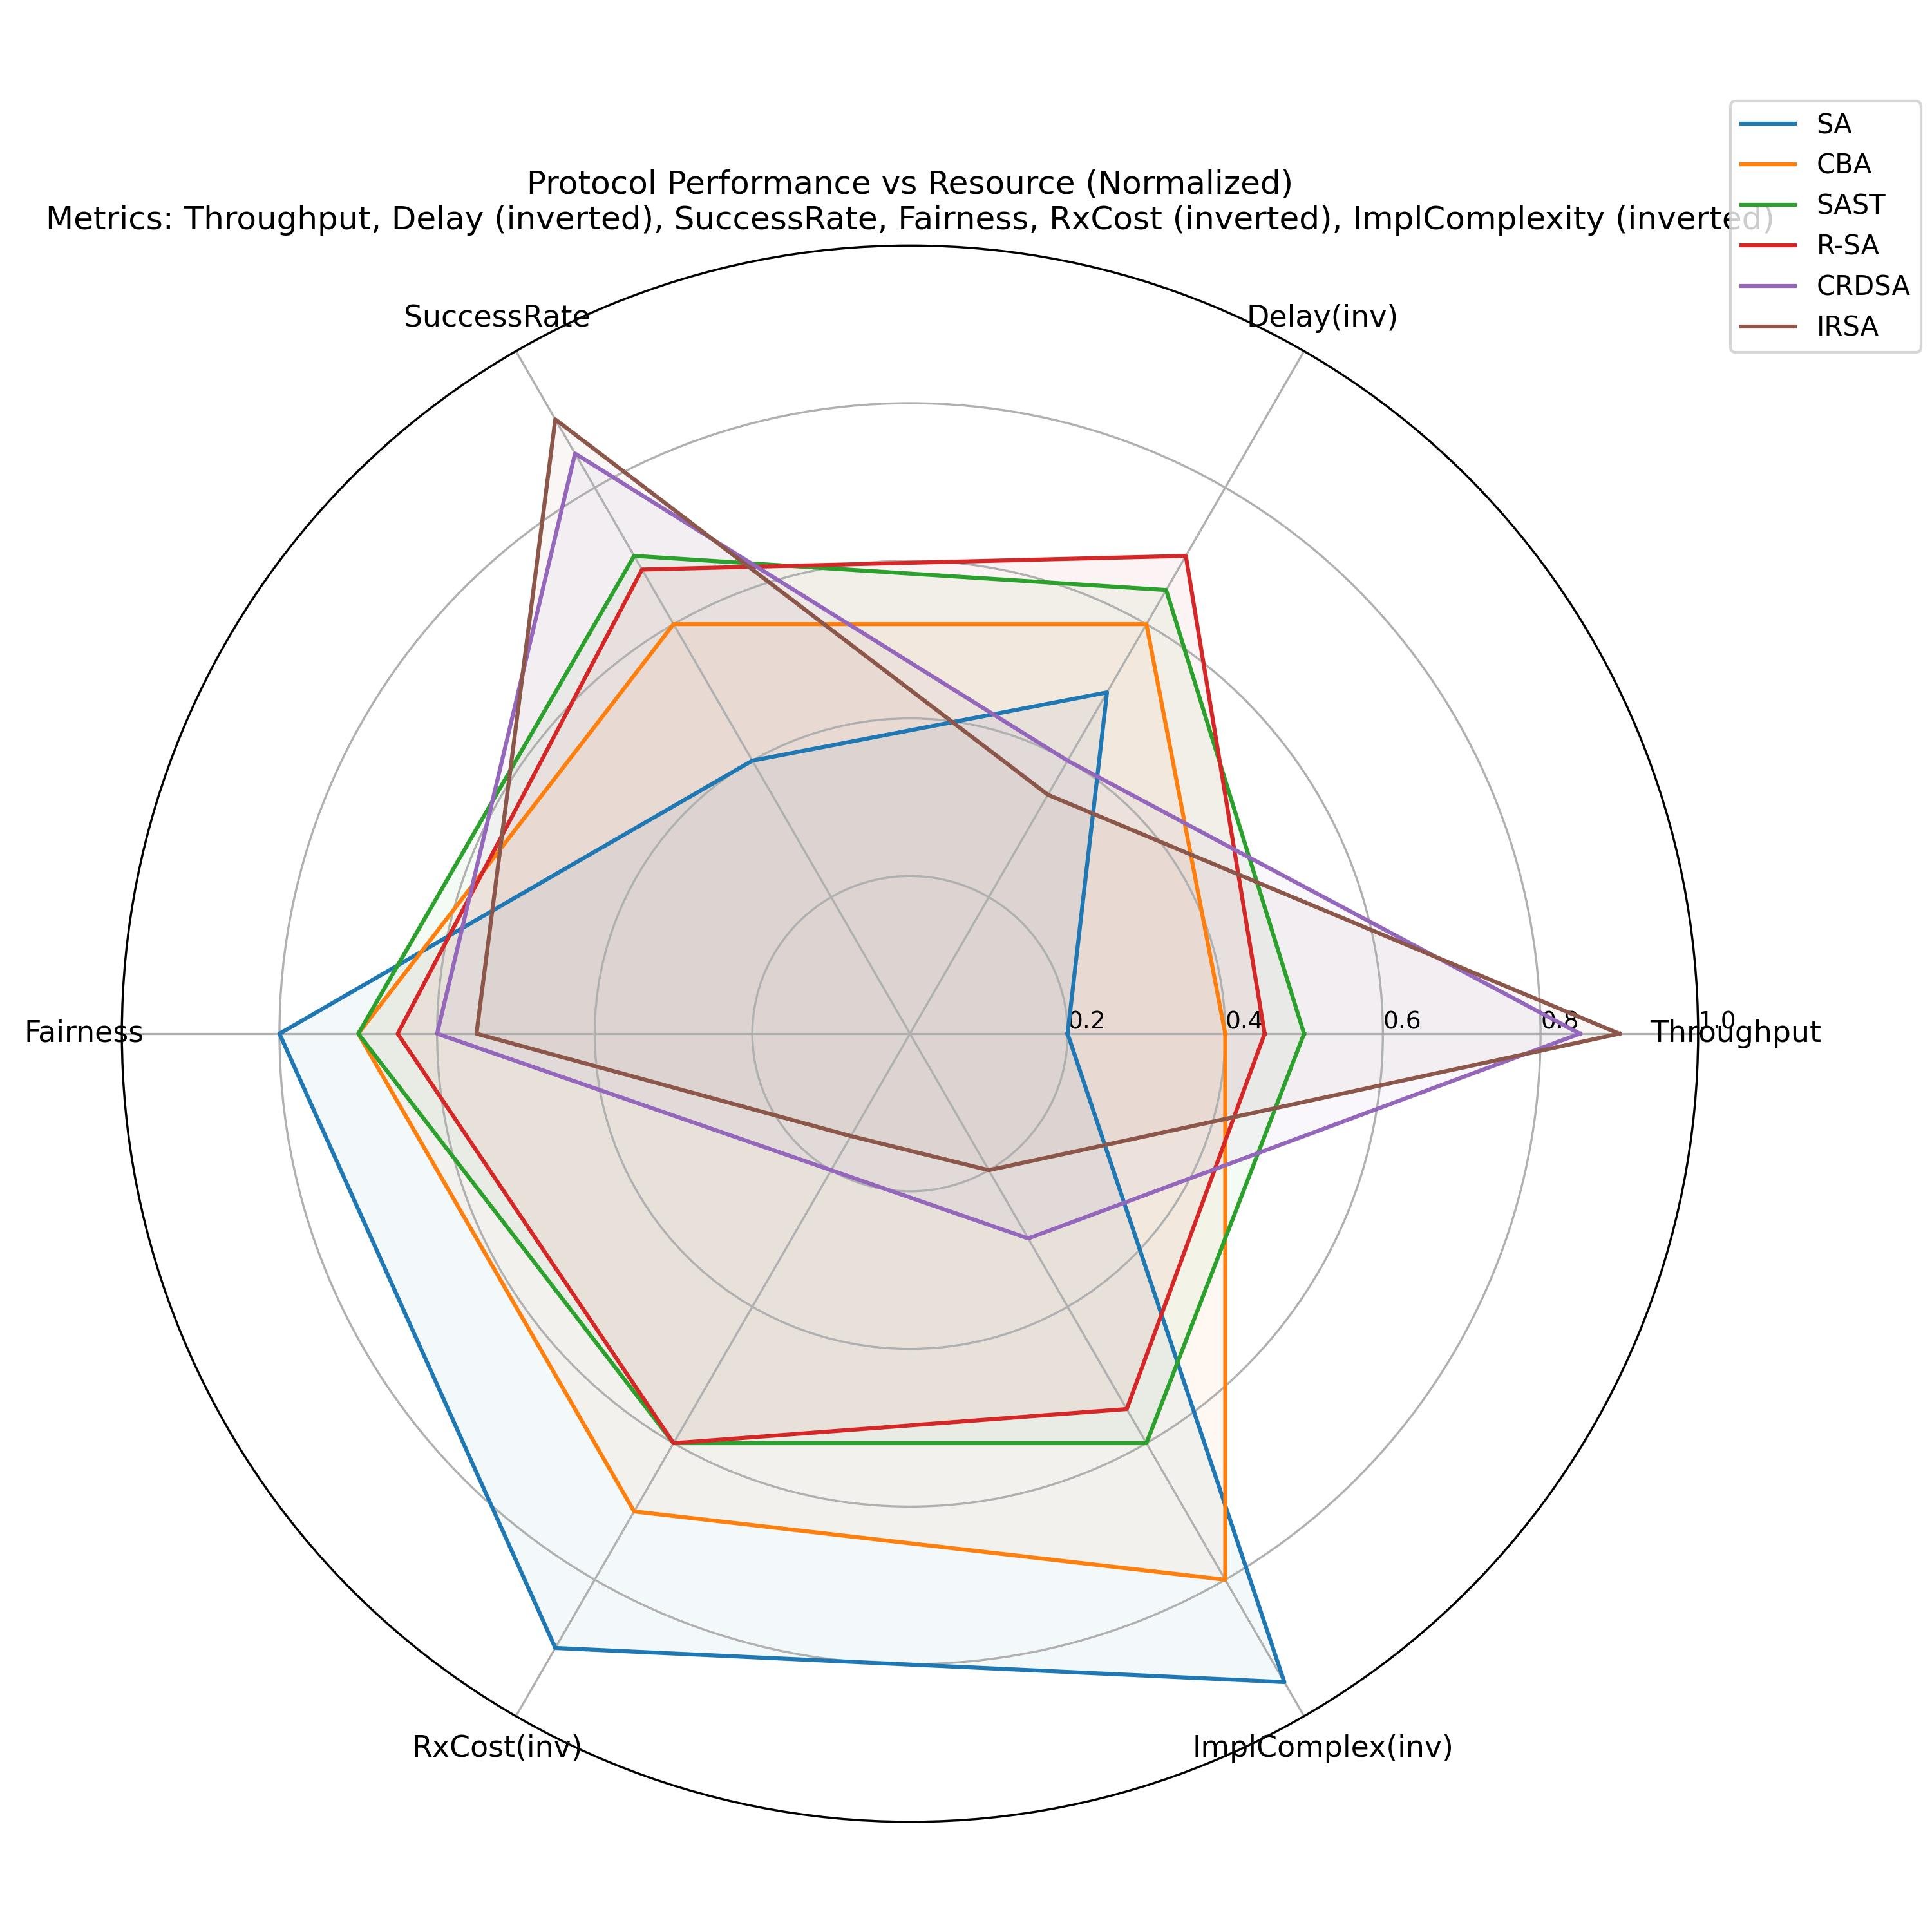
\includegraphics[width=0.3\textwidth]{figure/chap5/Sim11.jpg}
% 		\label{fig:protocol_throughput_comparison1}
% 	}
% 	\hfill
% 	\subfloat[突发场景]{
% 		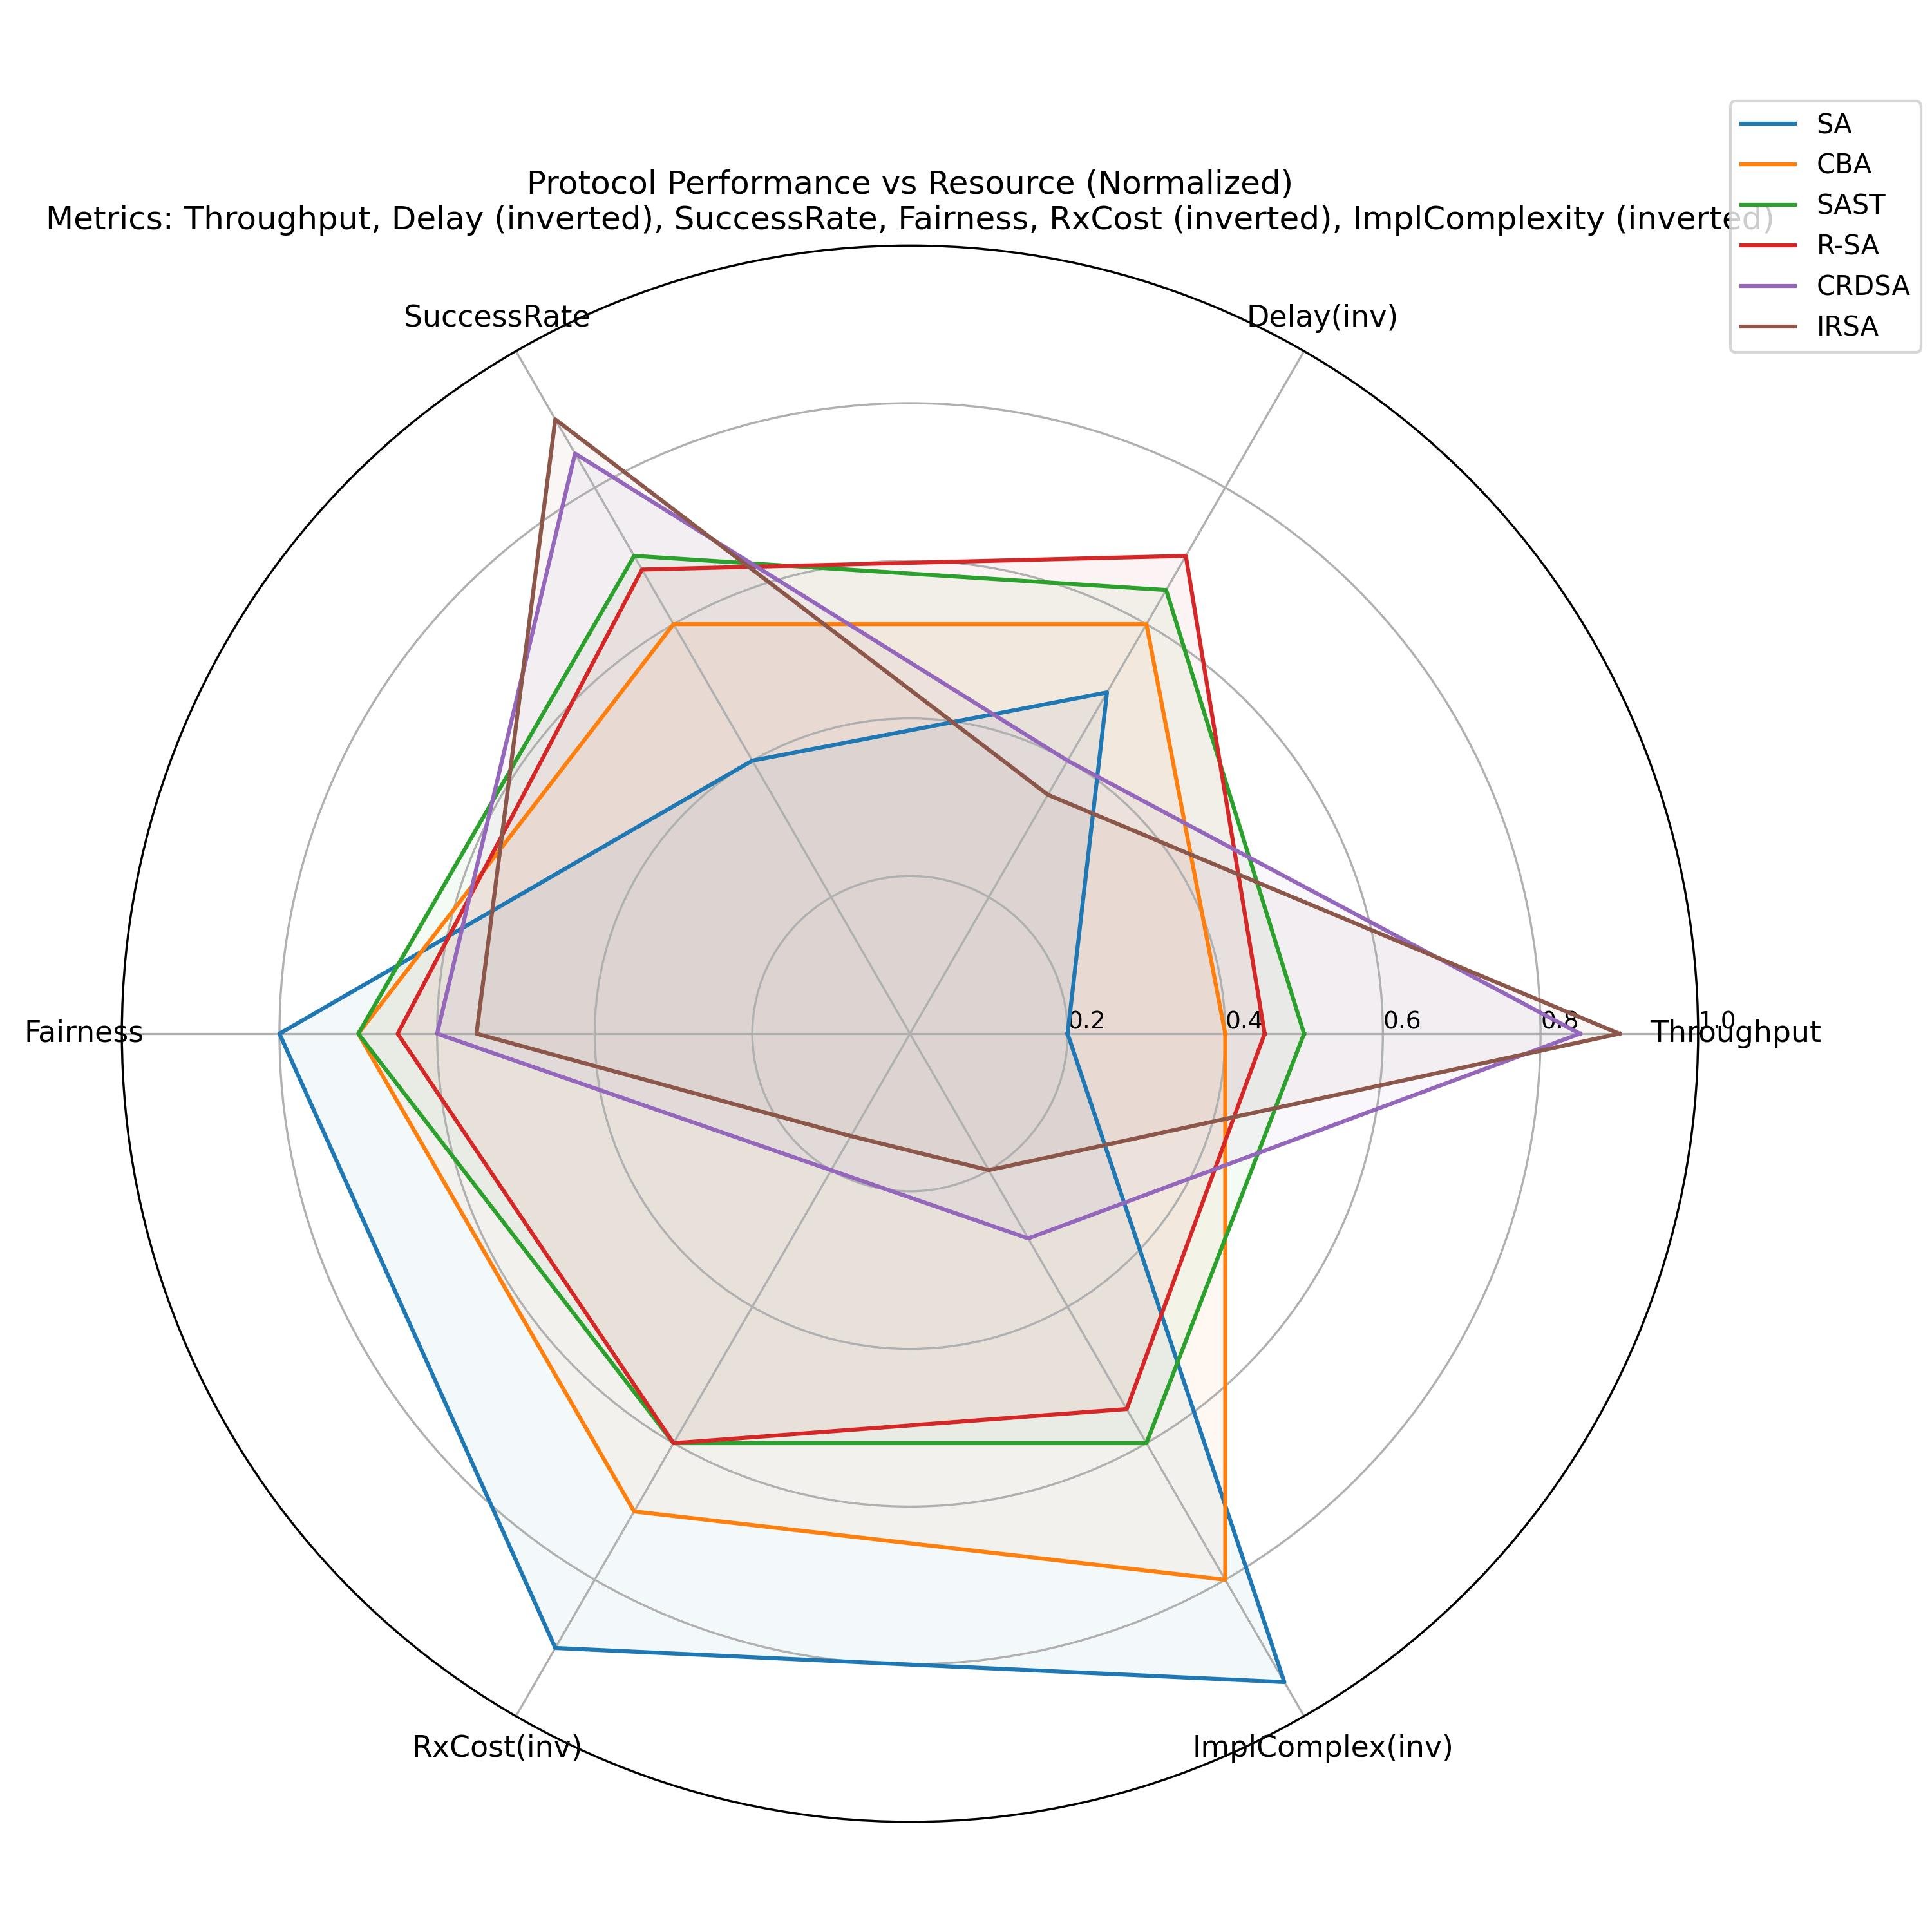
\includegraphics[width=0.3\textwidth]{figure/chap5/Sim12.jpg}
% 		\label{fig:protocol_throughput_comparison2}
% 	}
% 	\hfill
% 	\subfloat[周期场景]{
% 		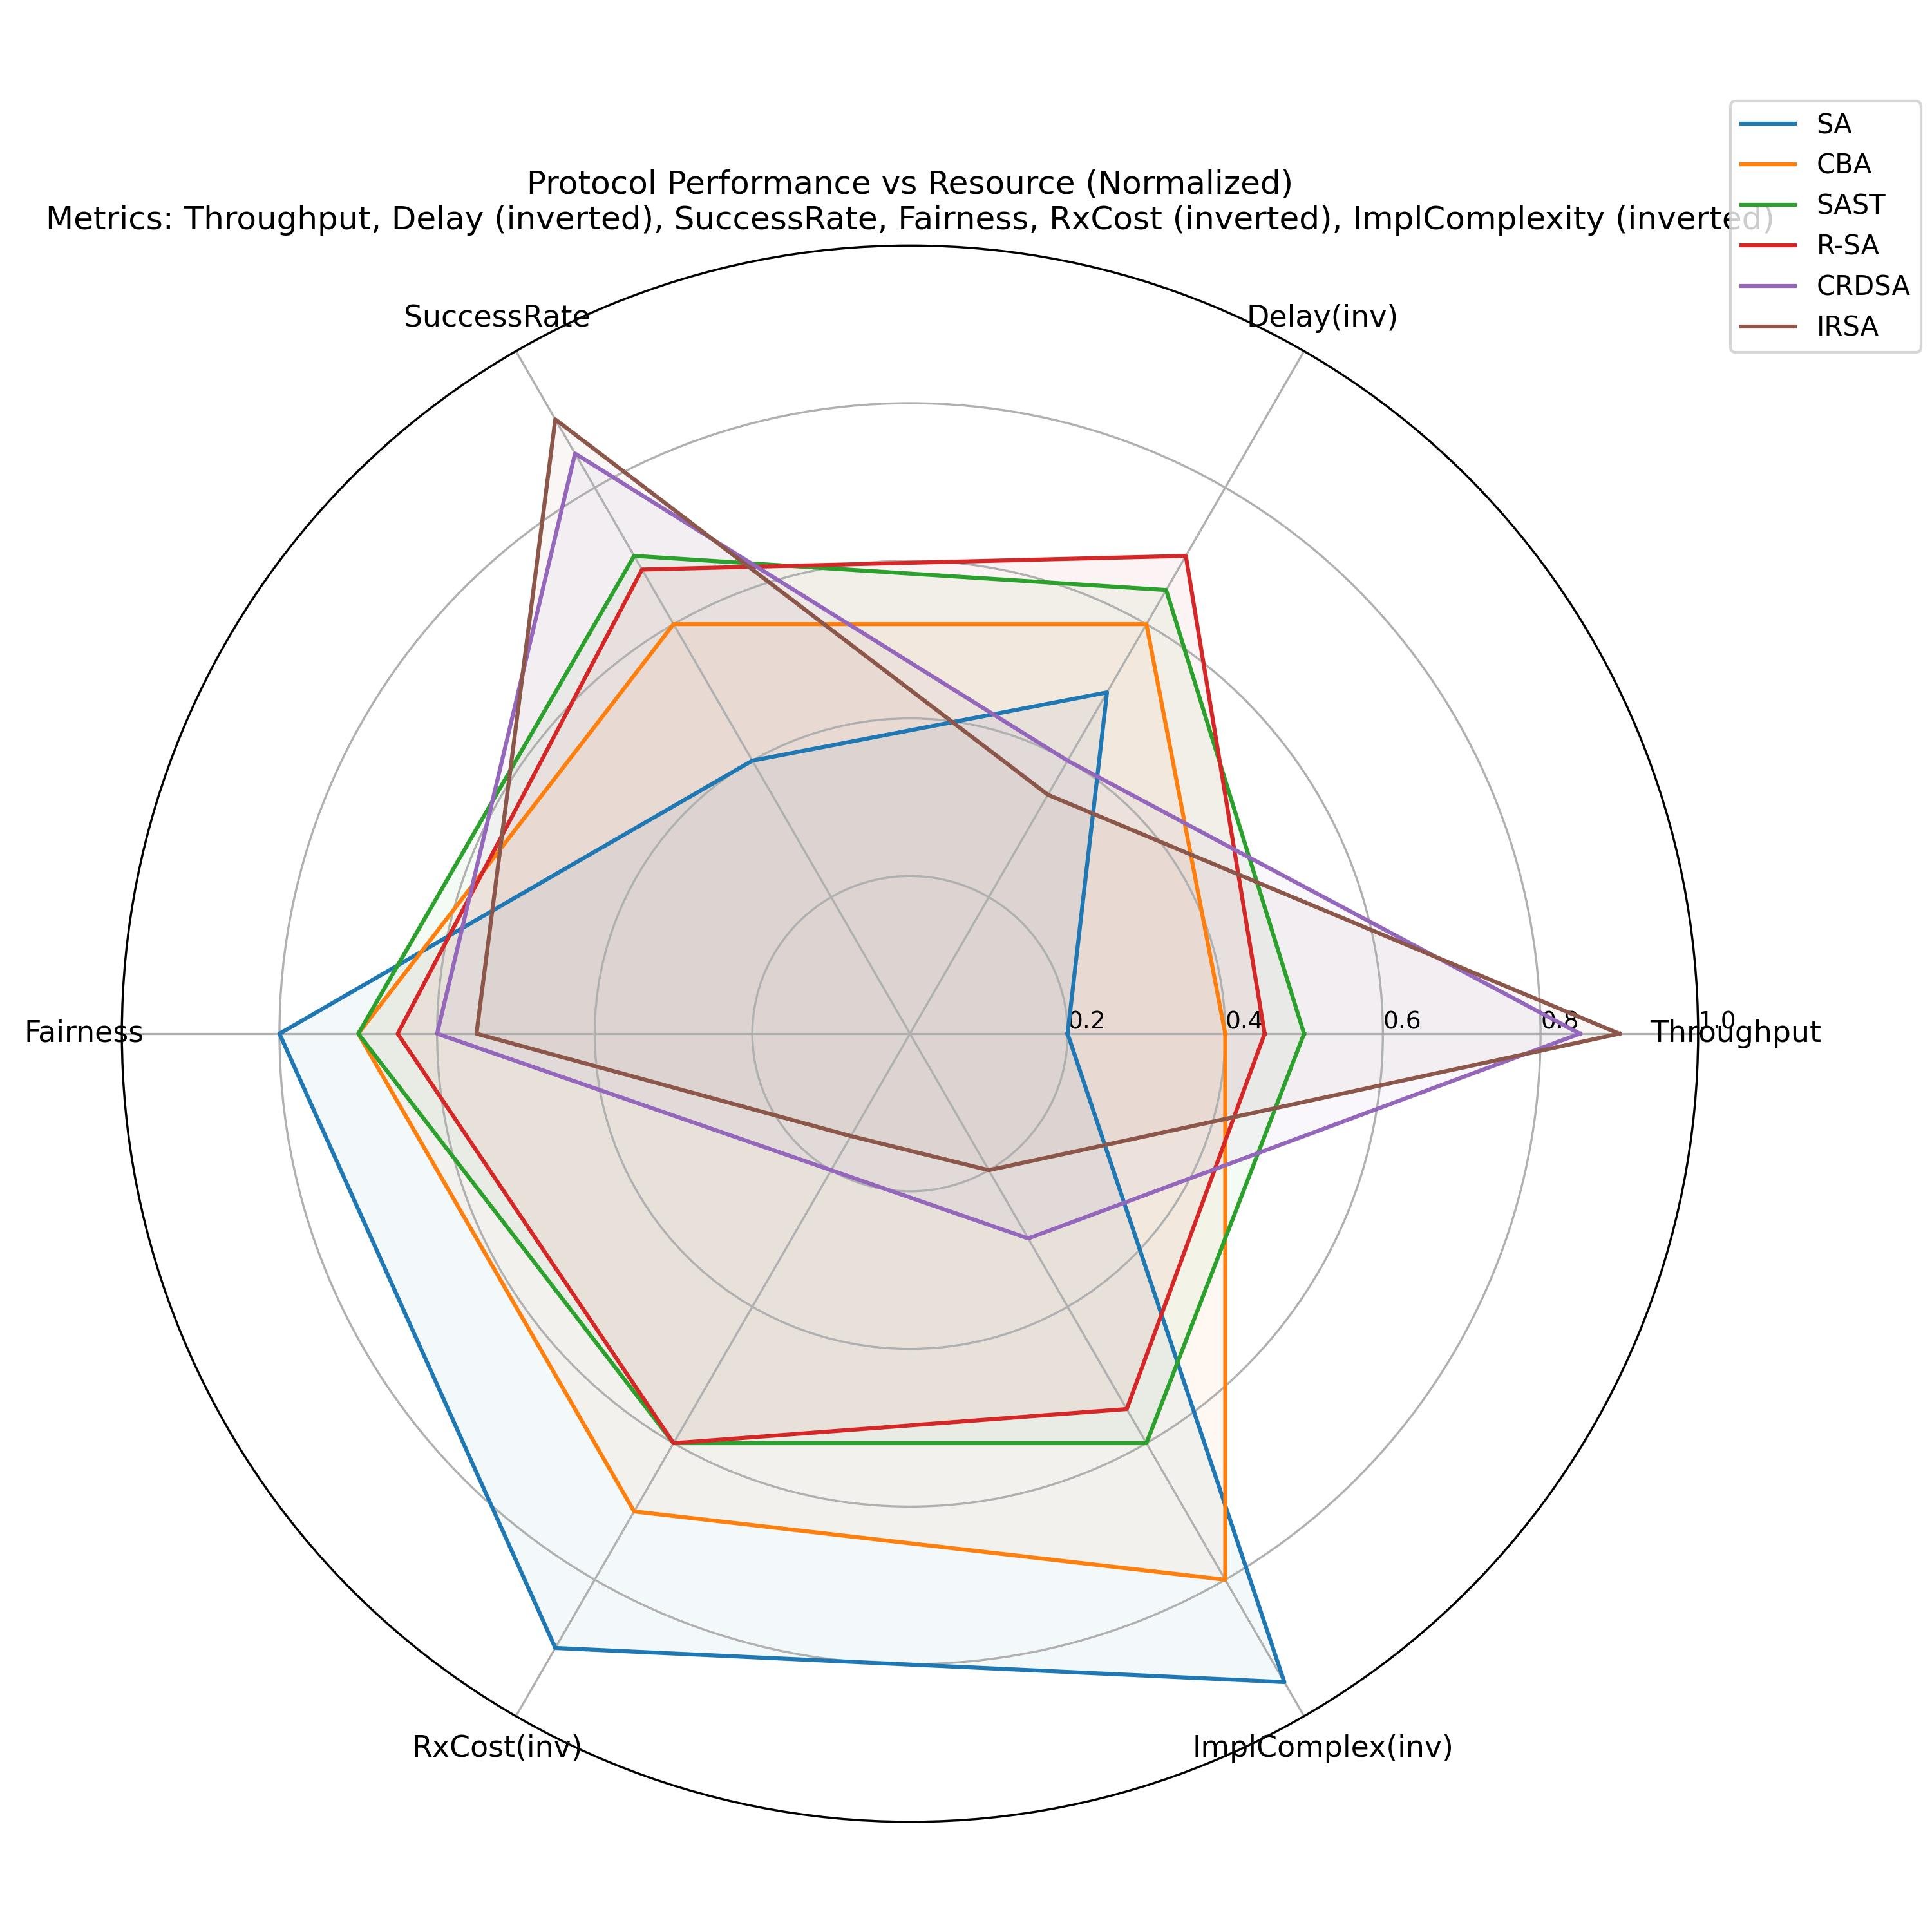
\includegraphics[width=0.3\textwidth]{figure/chap5/Sim13.jpg}
% 		\label{fig:protocol_throughput_comparison3}
% 	}
% 	\caption{不同协议在传输概率变化下的吞吐量对比（固定平均到达率为 $\hat{\lambda}=0.3$）。}
% 	\label{fig:protocol_throughput_comparison}
% \end{figure}

% \textbf{时延对比。} 
% 图~\ref{fig:protocol_delay_comparison} 展示了平均时延 $D$ 随 $\hat{\lambda}$ 的变化趋势。

% \begin{figure}[t]
% 	\centering
% 	\subfloat[均匀场景]{
% 		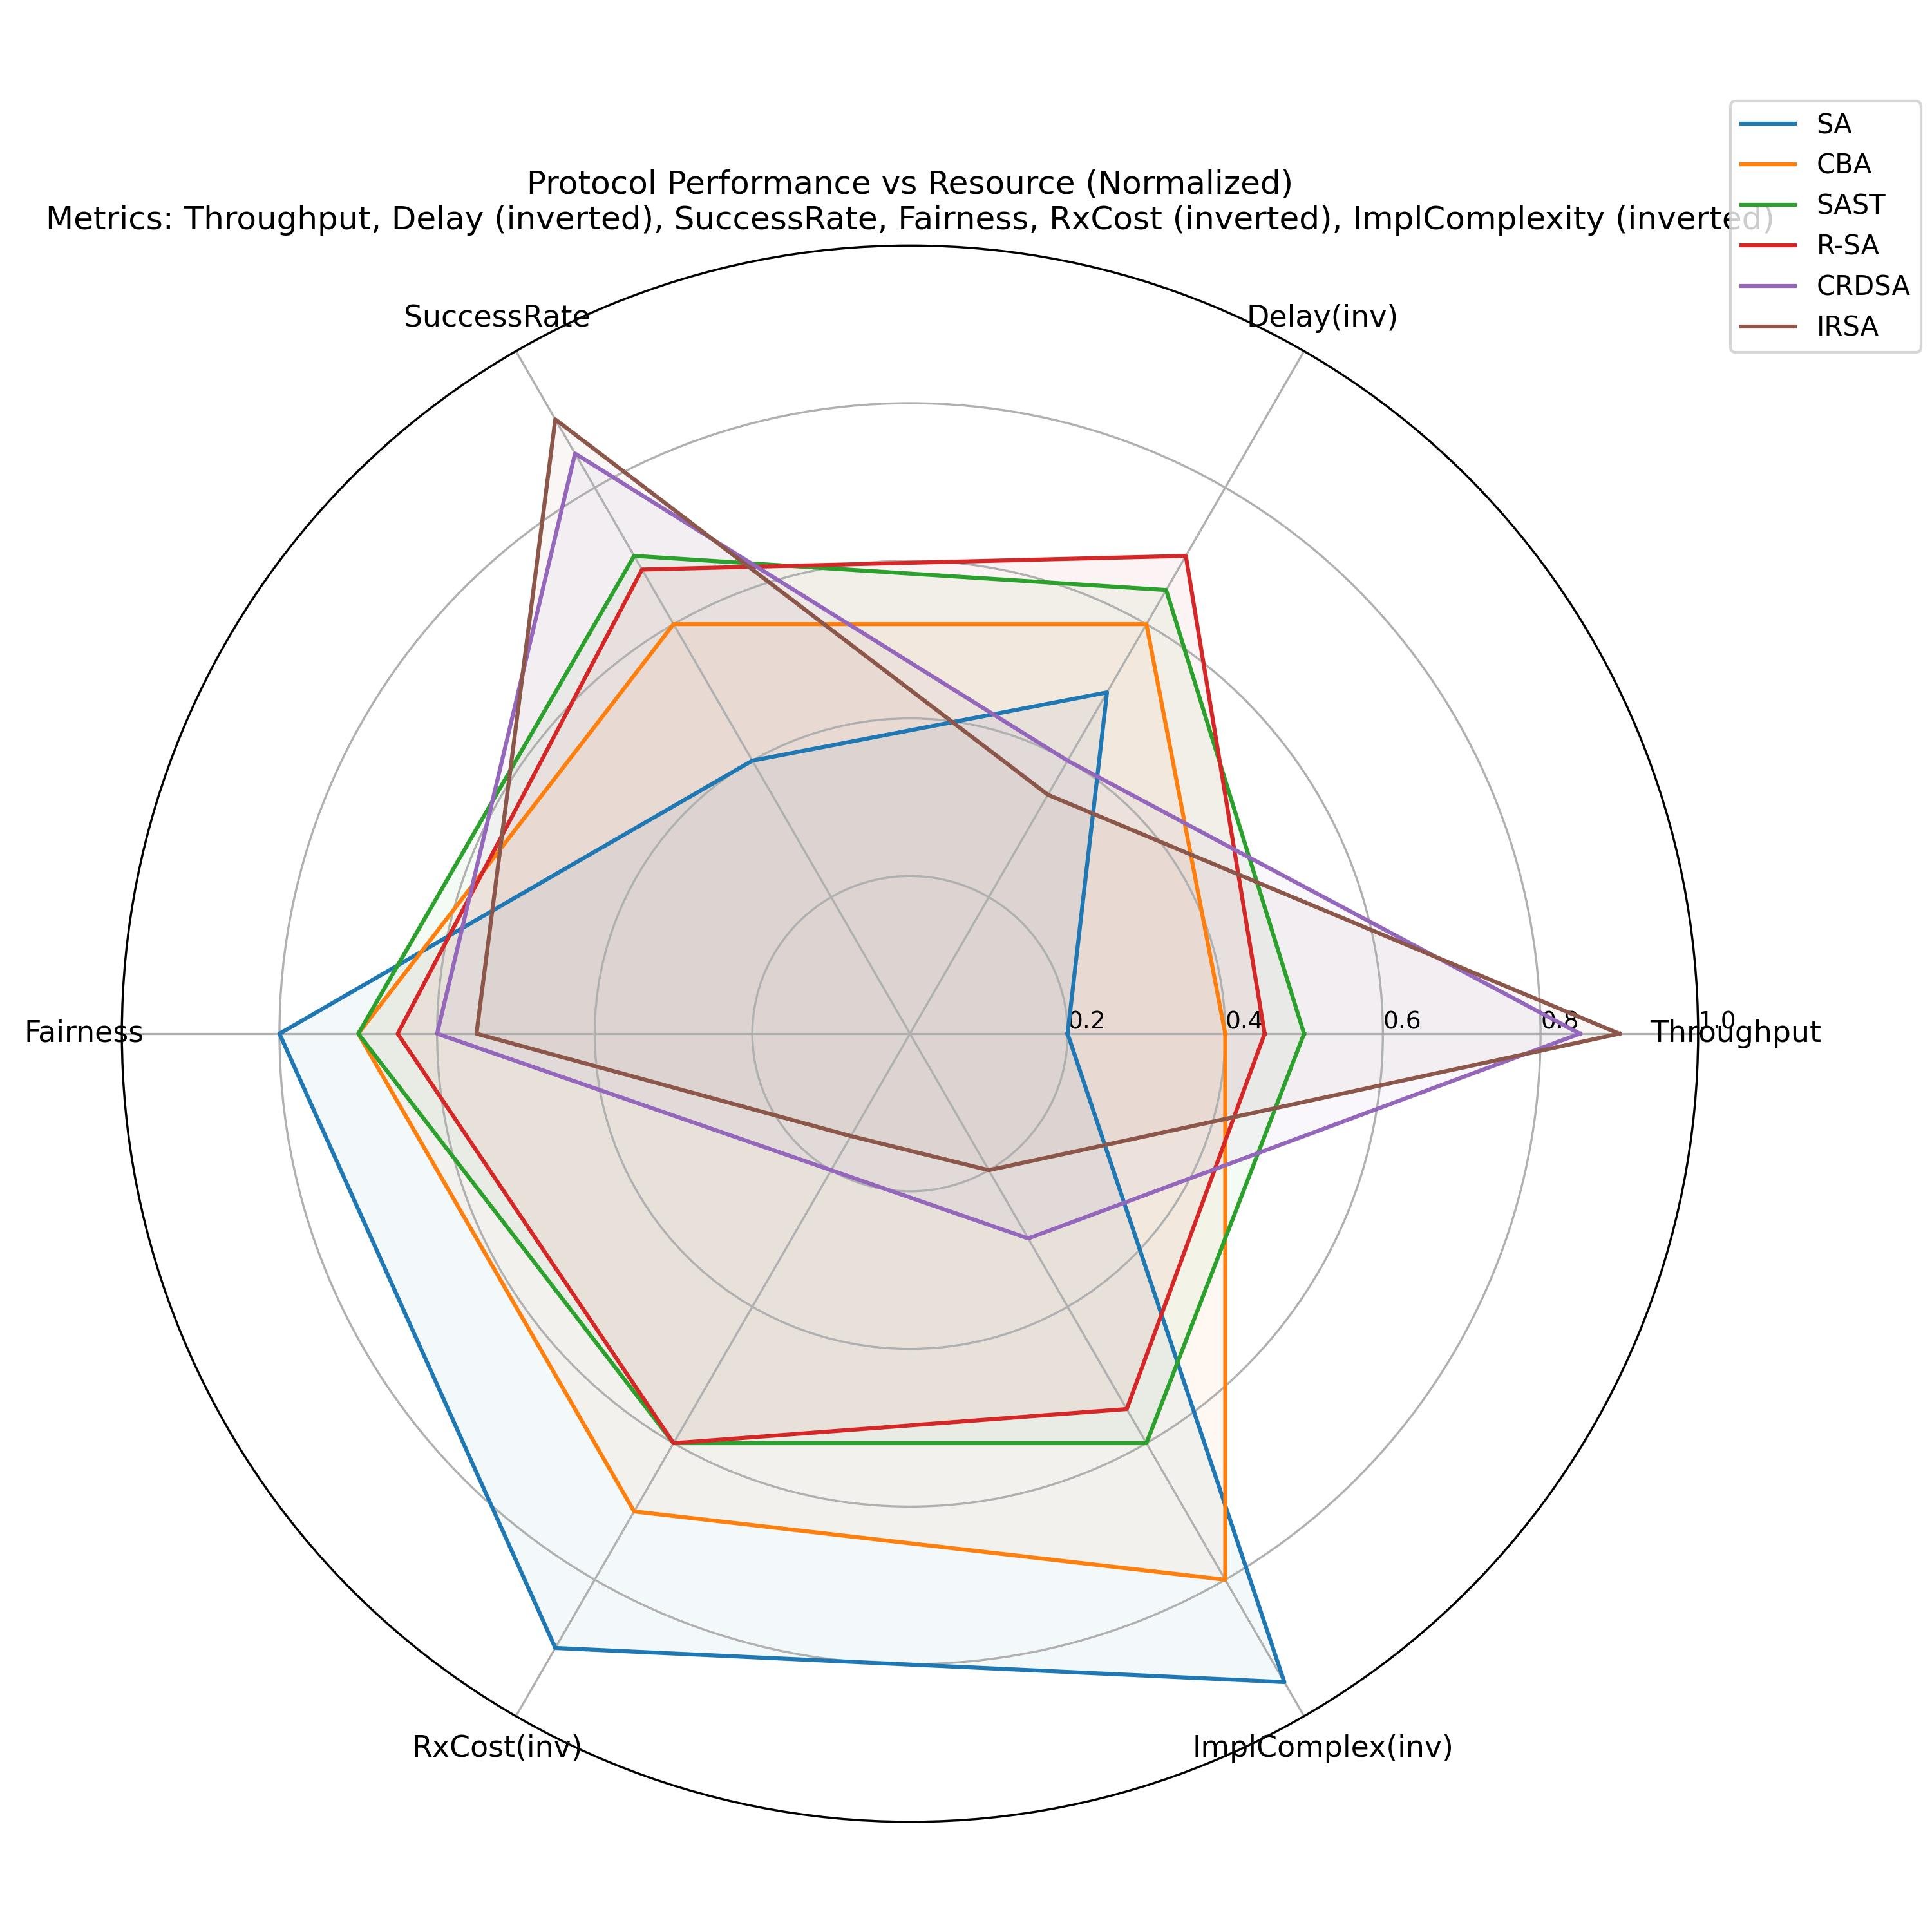
\includegraphics[width=0.3\textwidth]{figure/chap5/Sim21.jpg}
% 		\label{fig:protocol_delay_comparison1}
% 	}
% 	\hfill
% 	\subfloat[突发场景]{
% 		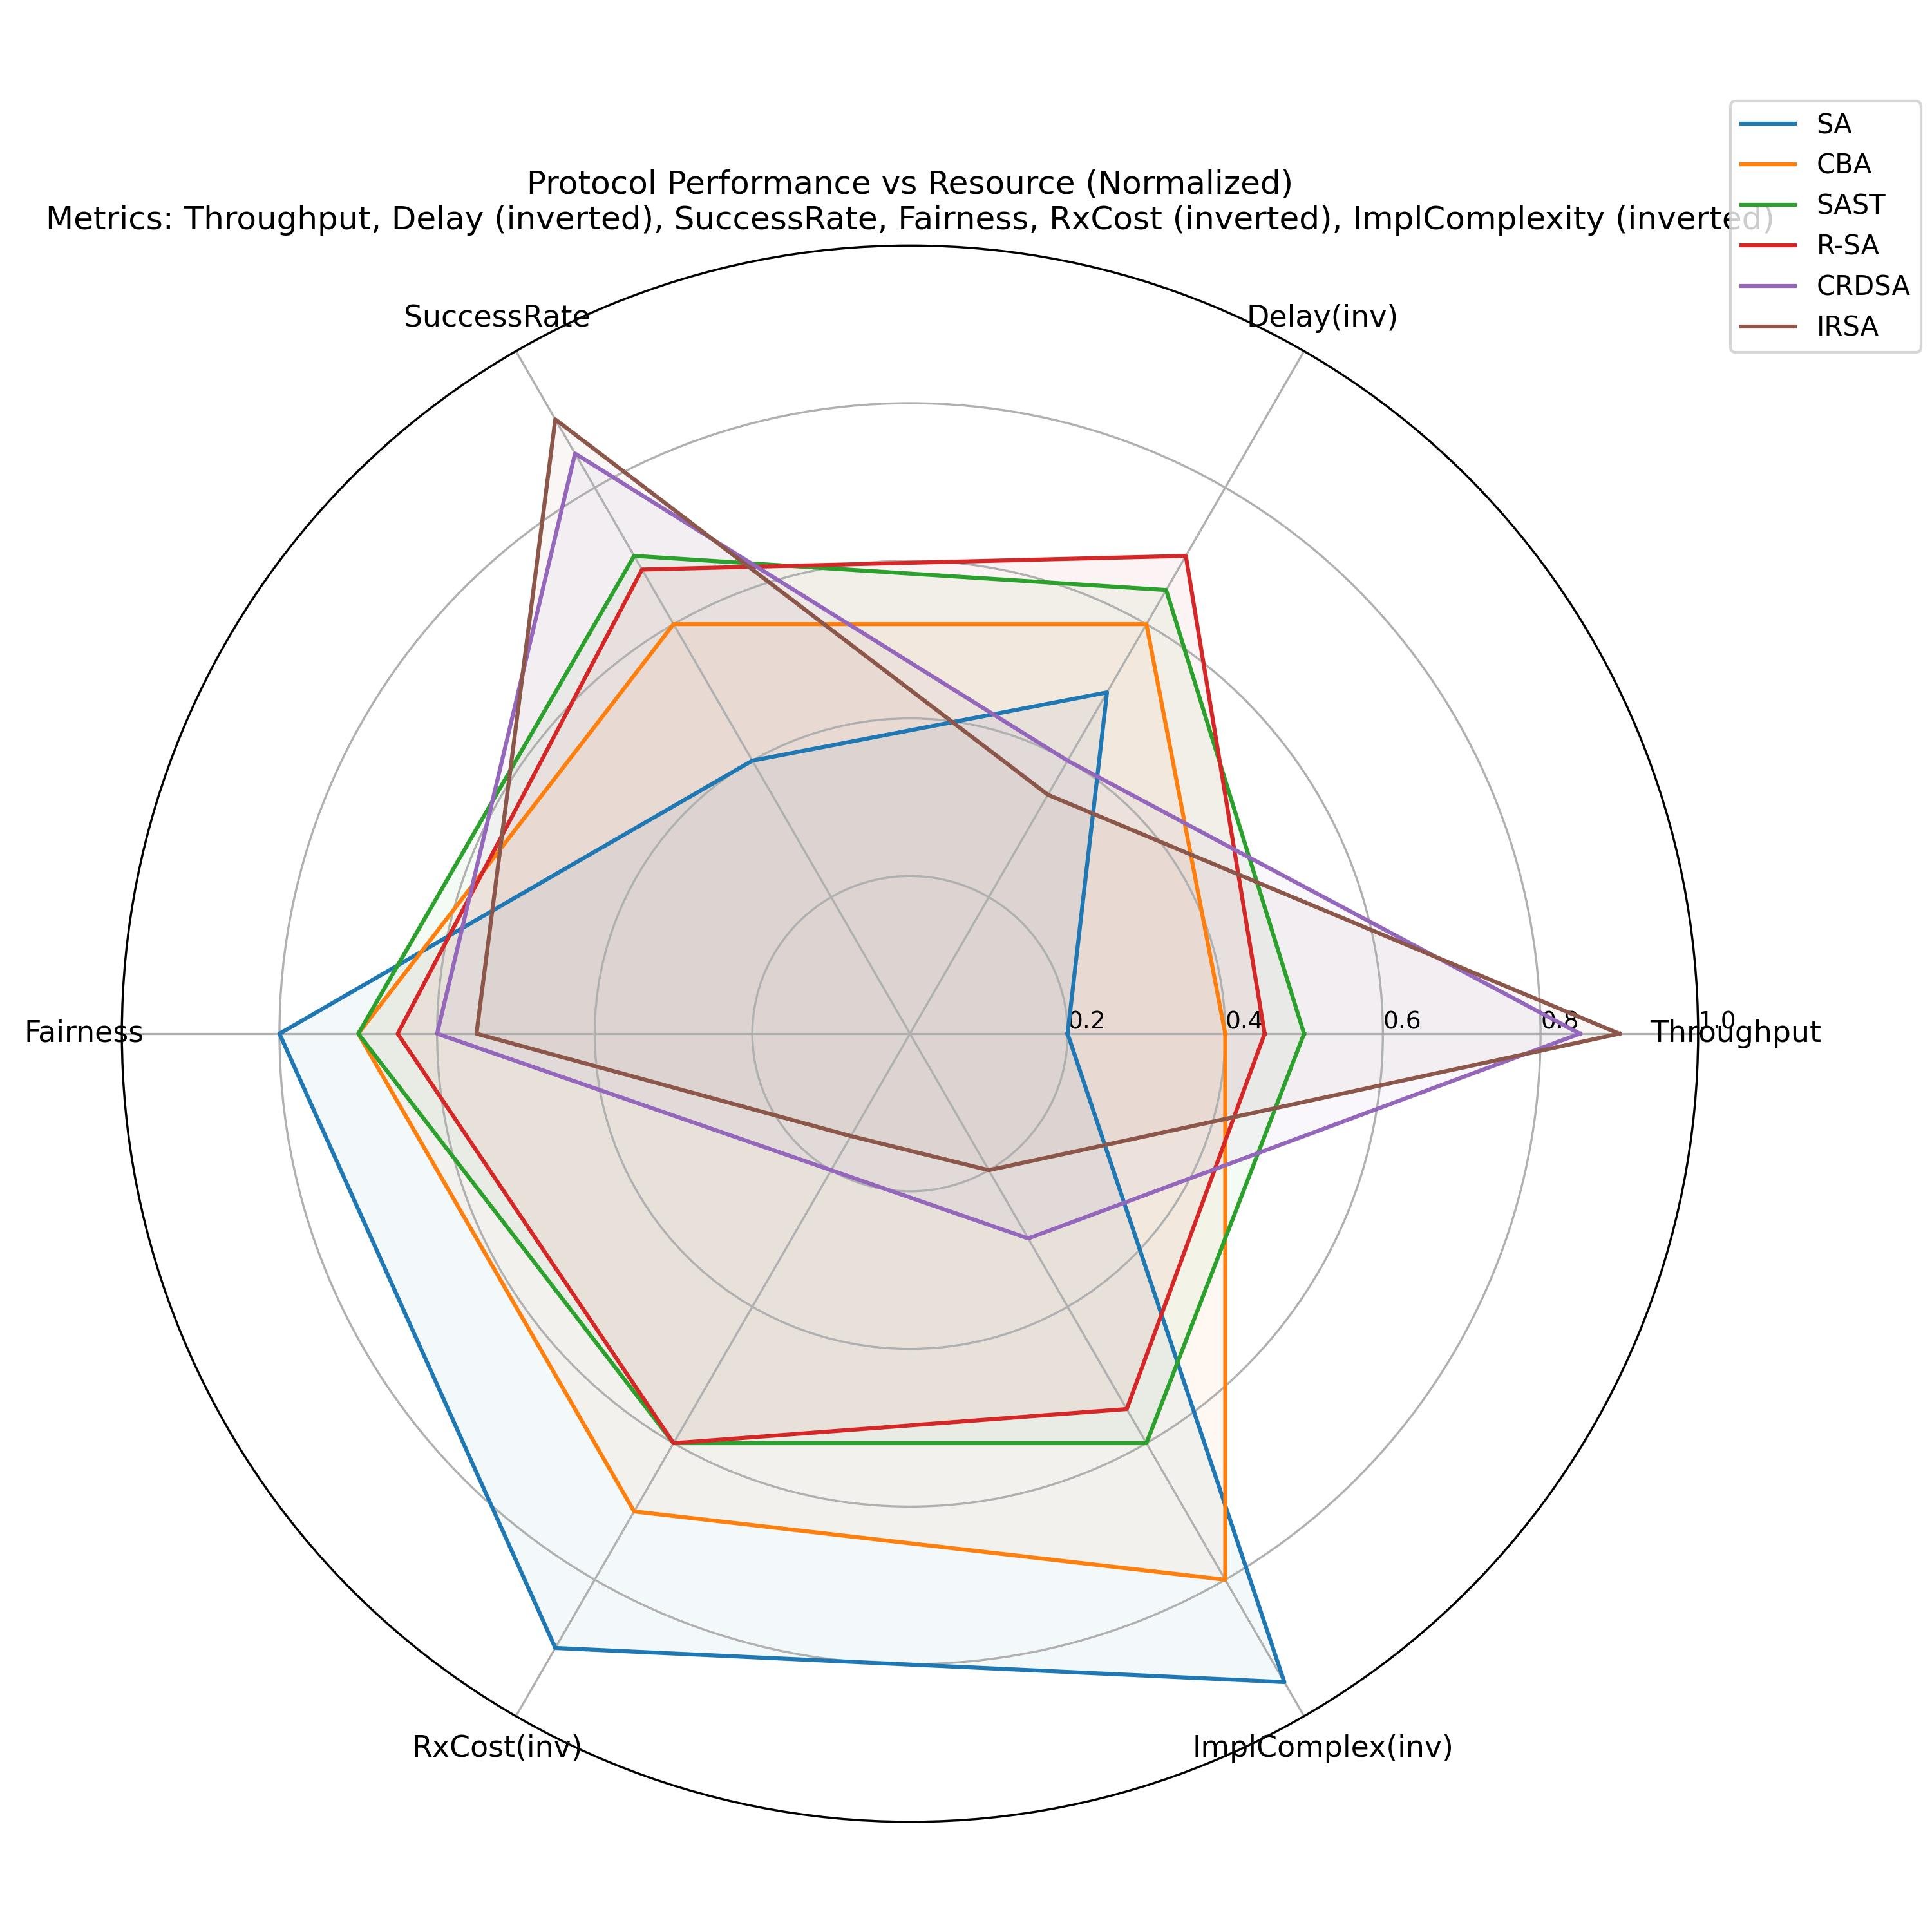
\includegraphics[width=0.3\textwidth]{figure/chap5/Sim22.jpg}
% 		\label{fig:protocol_delay_comparison2}
% 	}
% 	\hfill
% 	\subfloat[周期场景]{
% 		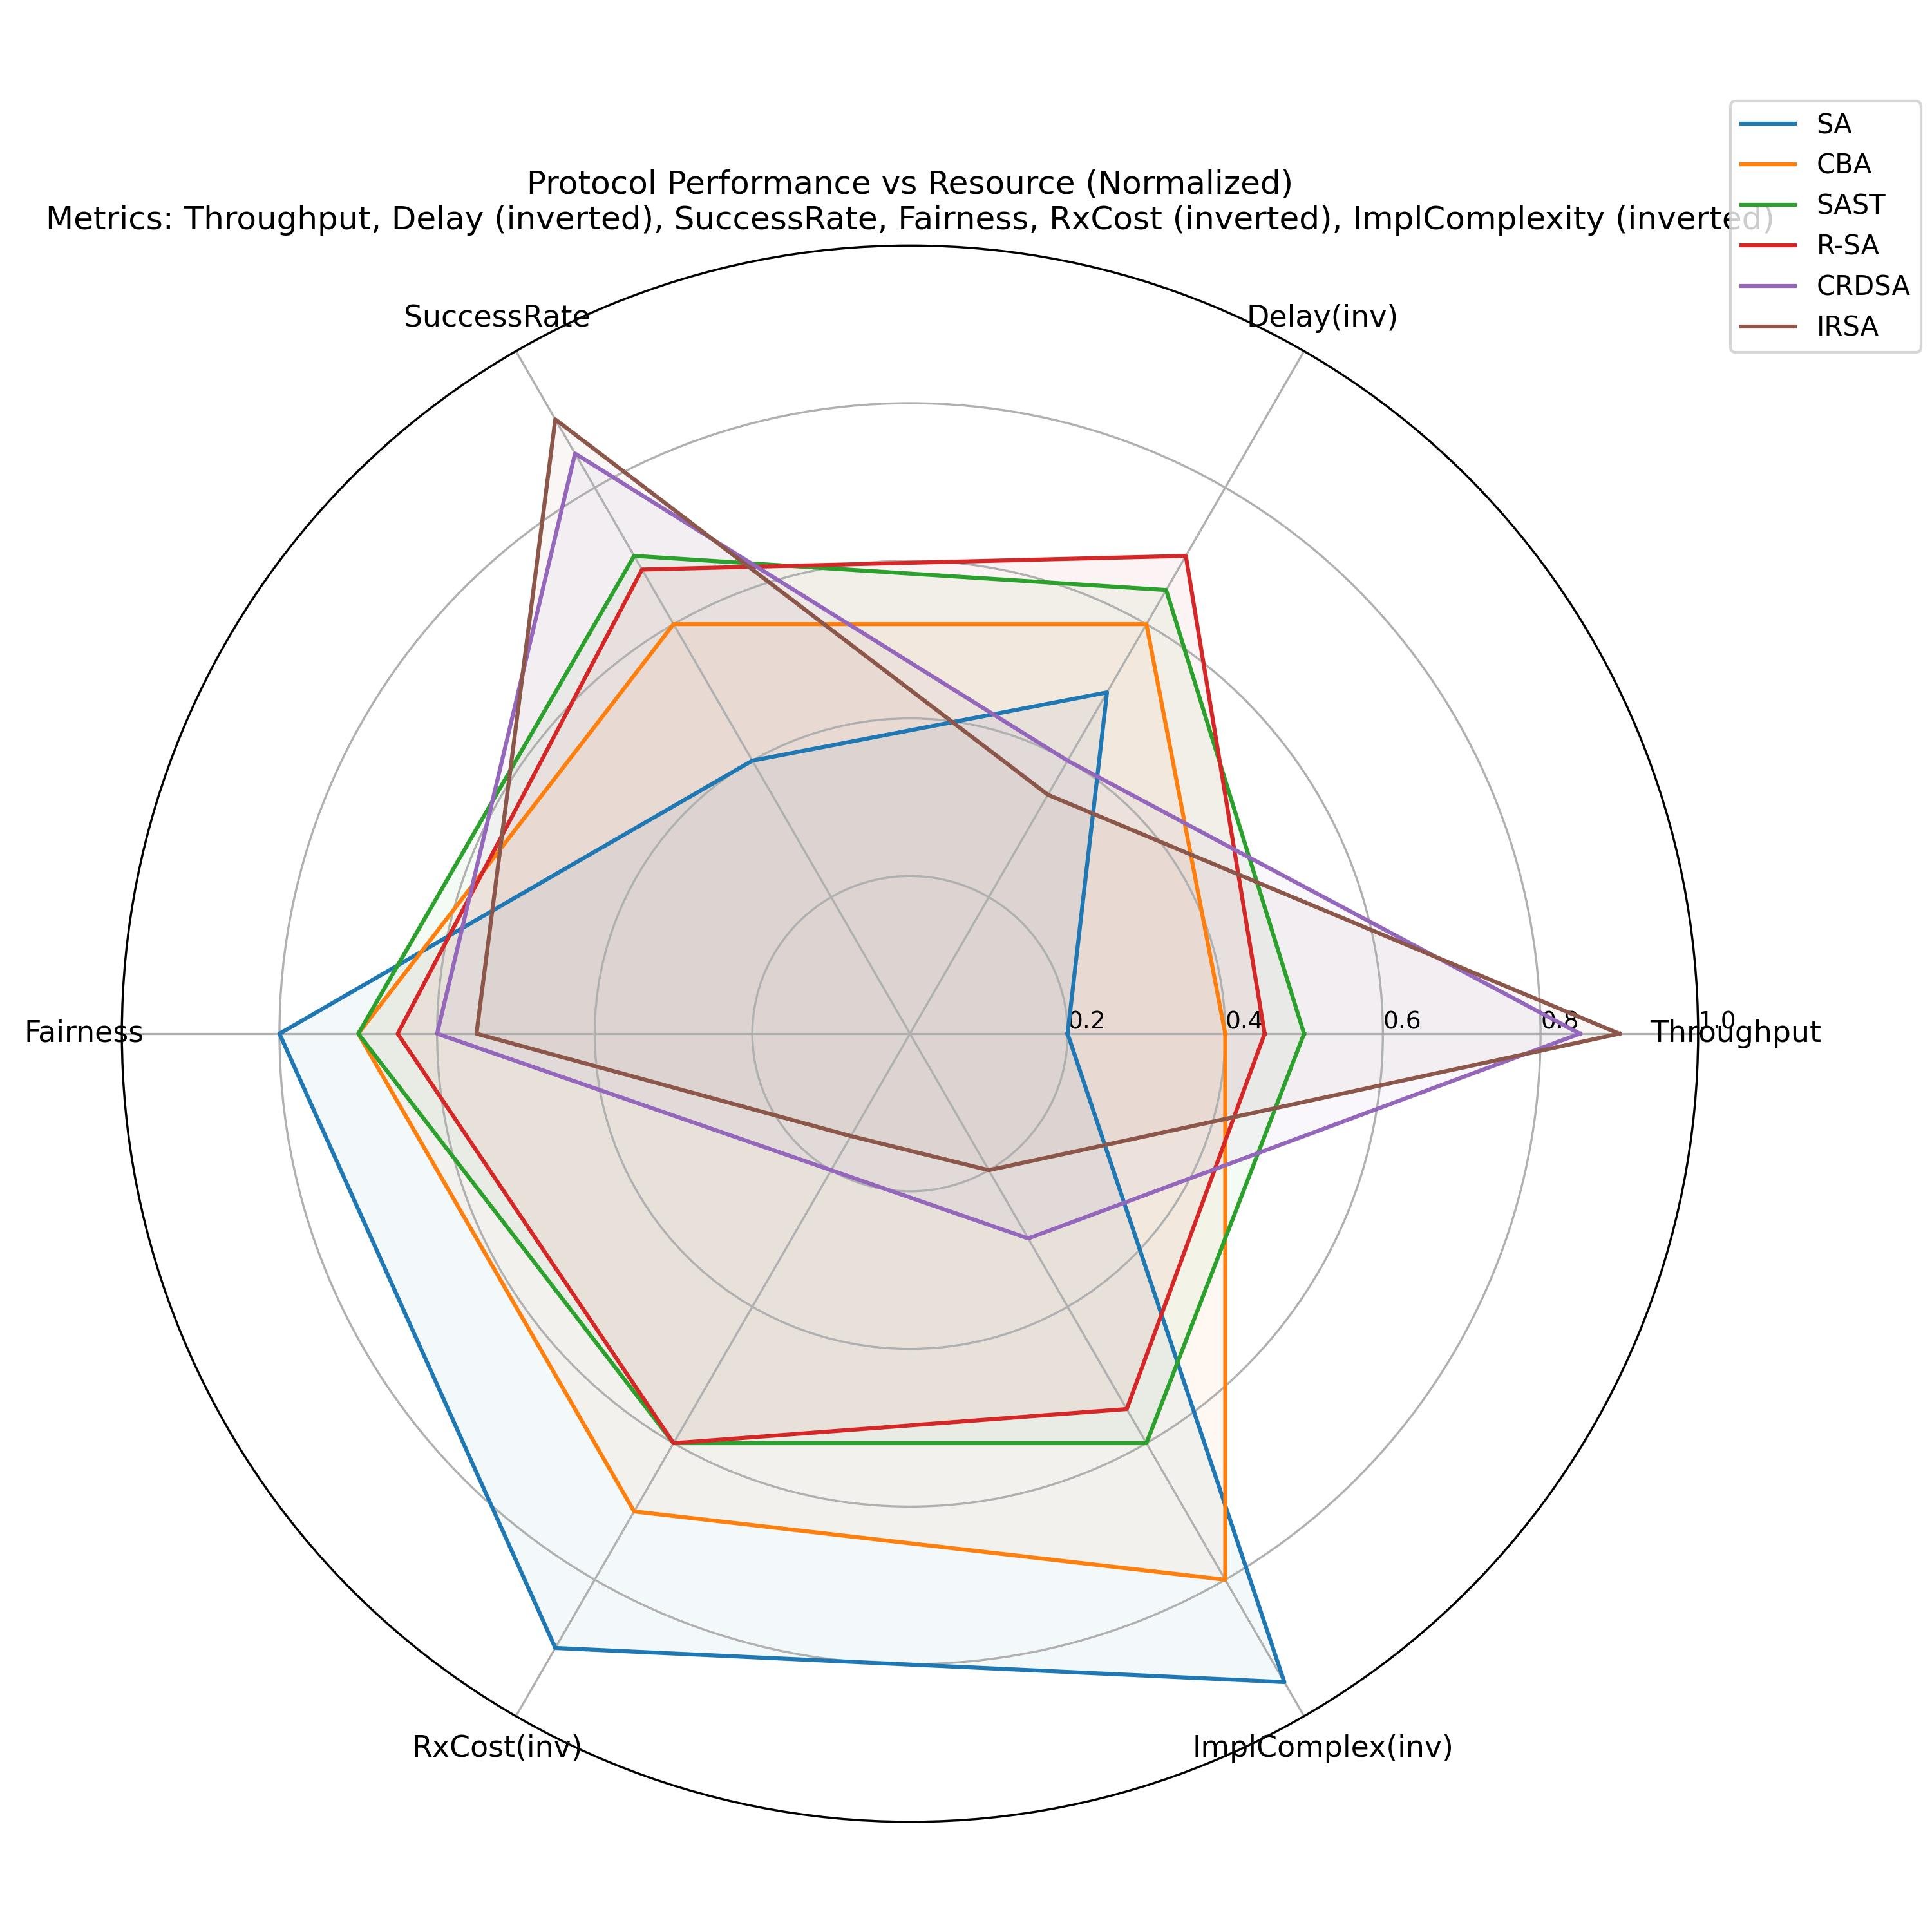
\includegraphics[width=0.3\textwidth]{figure/chap5/Sim23.jpg}
% 		\label{fig:protocol_delay_comparison3}
% 	}
% 	\caption{不同协议在传输概率变化下的平均时延对比（固定平均到达率为 $\hat{\lambda}=0.3$）。}
% 	\label{fig:protocol_delay_comparison}
% \end{figure}


% \textbf{公平性评估。} 
% 图~\ref{fig:protocol_fairness_comparison} 给出了公平性指标（Jain 指数）在不同协议下的变化特征。
% \begin{figure}[t]
% 	\centering
% 	\subfloat[均匀场景]{
% 		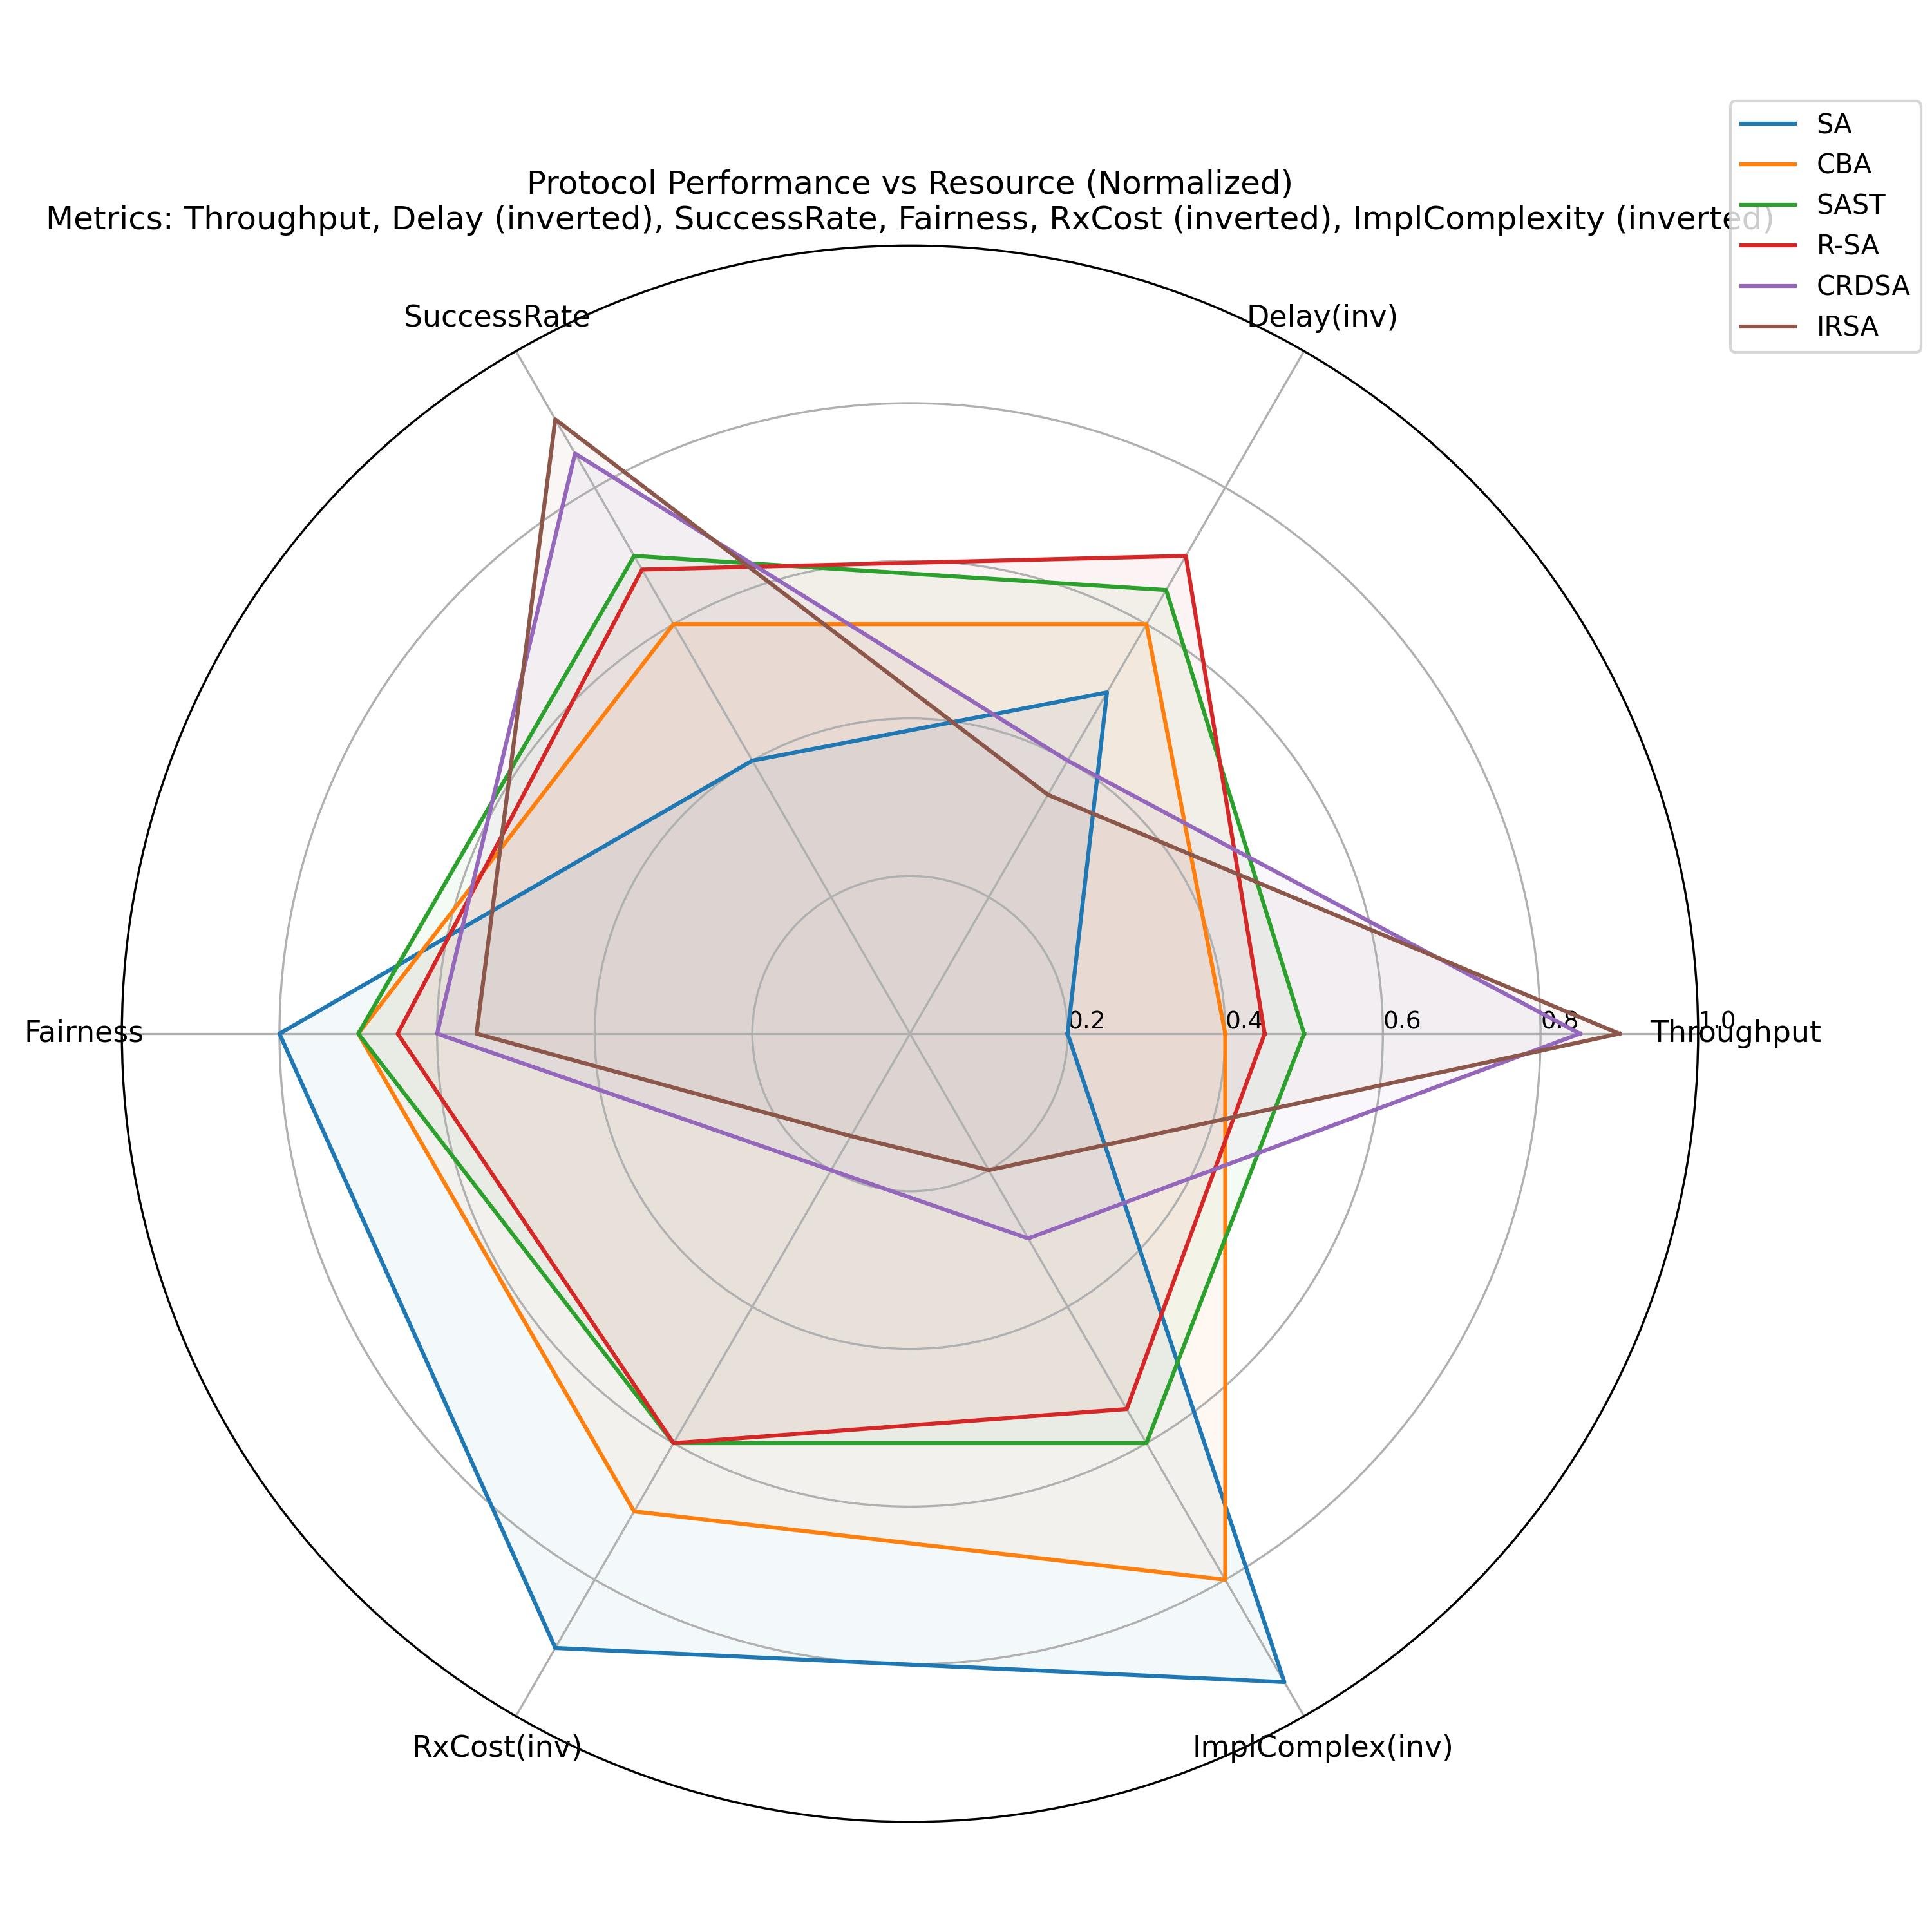
\includegraphics[width=0.3\textwidth]{figure/chap5/Sim31.jpg}
% 		\label{fig:protocol_fairness_comparison1}
% 	}
% 	\hfill
% 	\subfloat[突发场景]{
% 		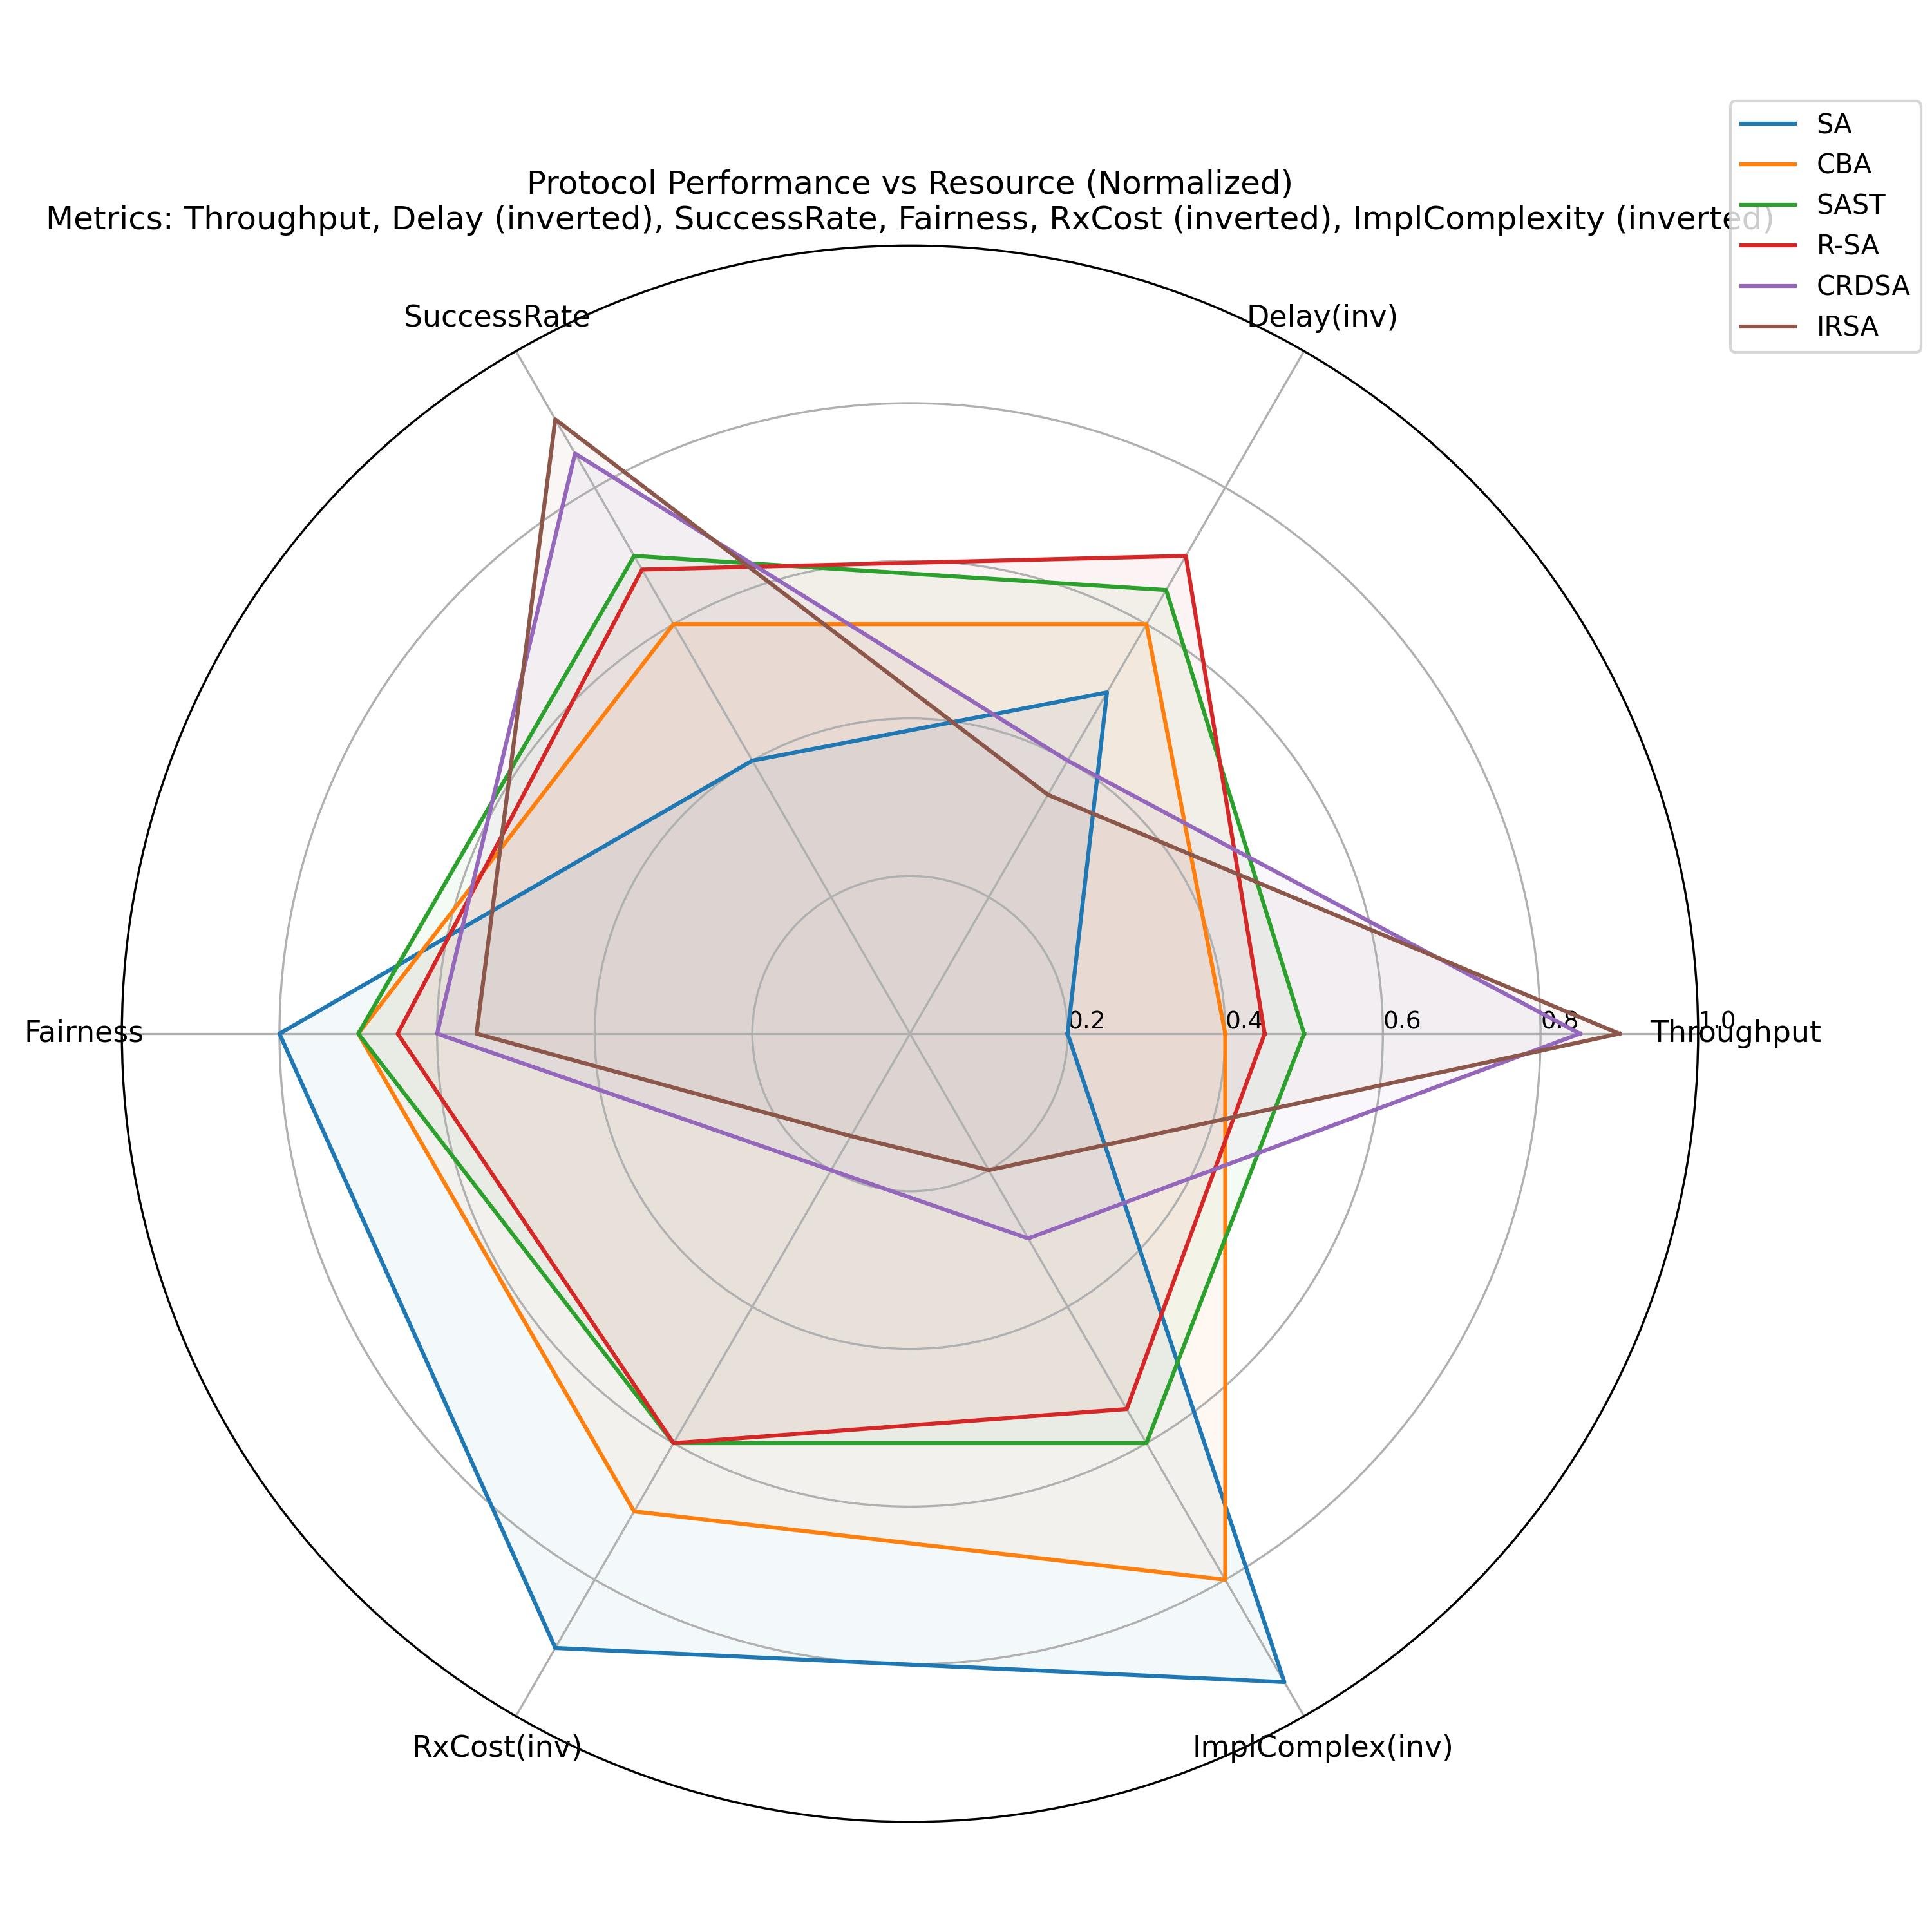
\includegraphics[width=0.3\textwidth]{figure/chap5/Sim32.jpg}
% 		\label{fig:protocol_fairness_comparison2}
% 	}
% 	\hfill
% 	\subfloat[周期场景]{
% 		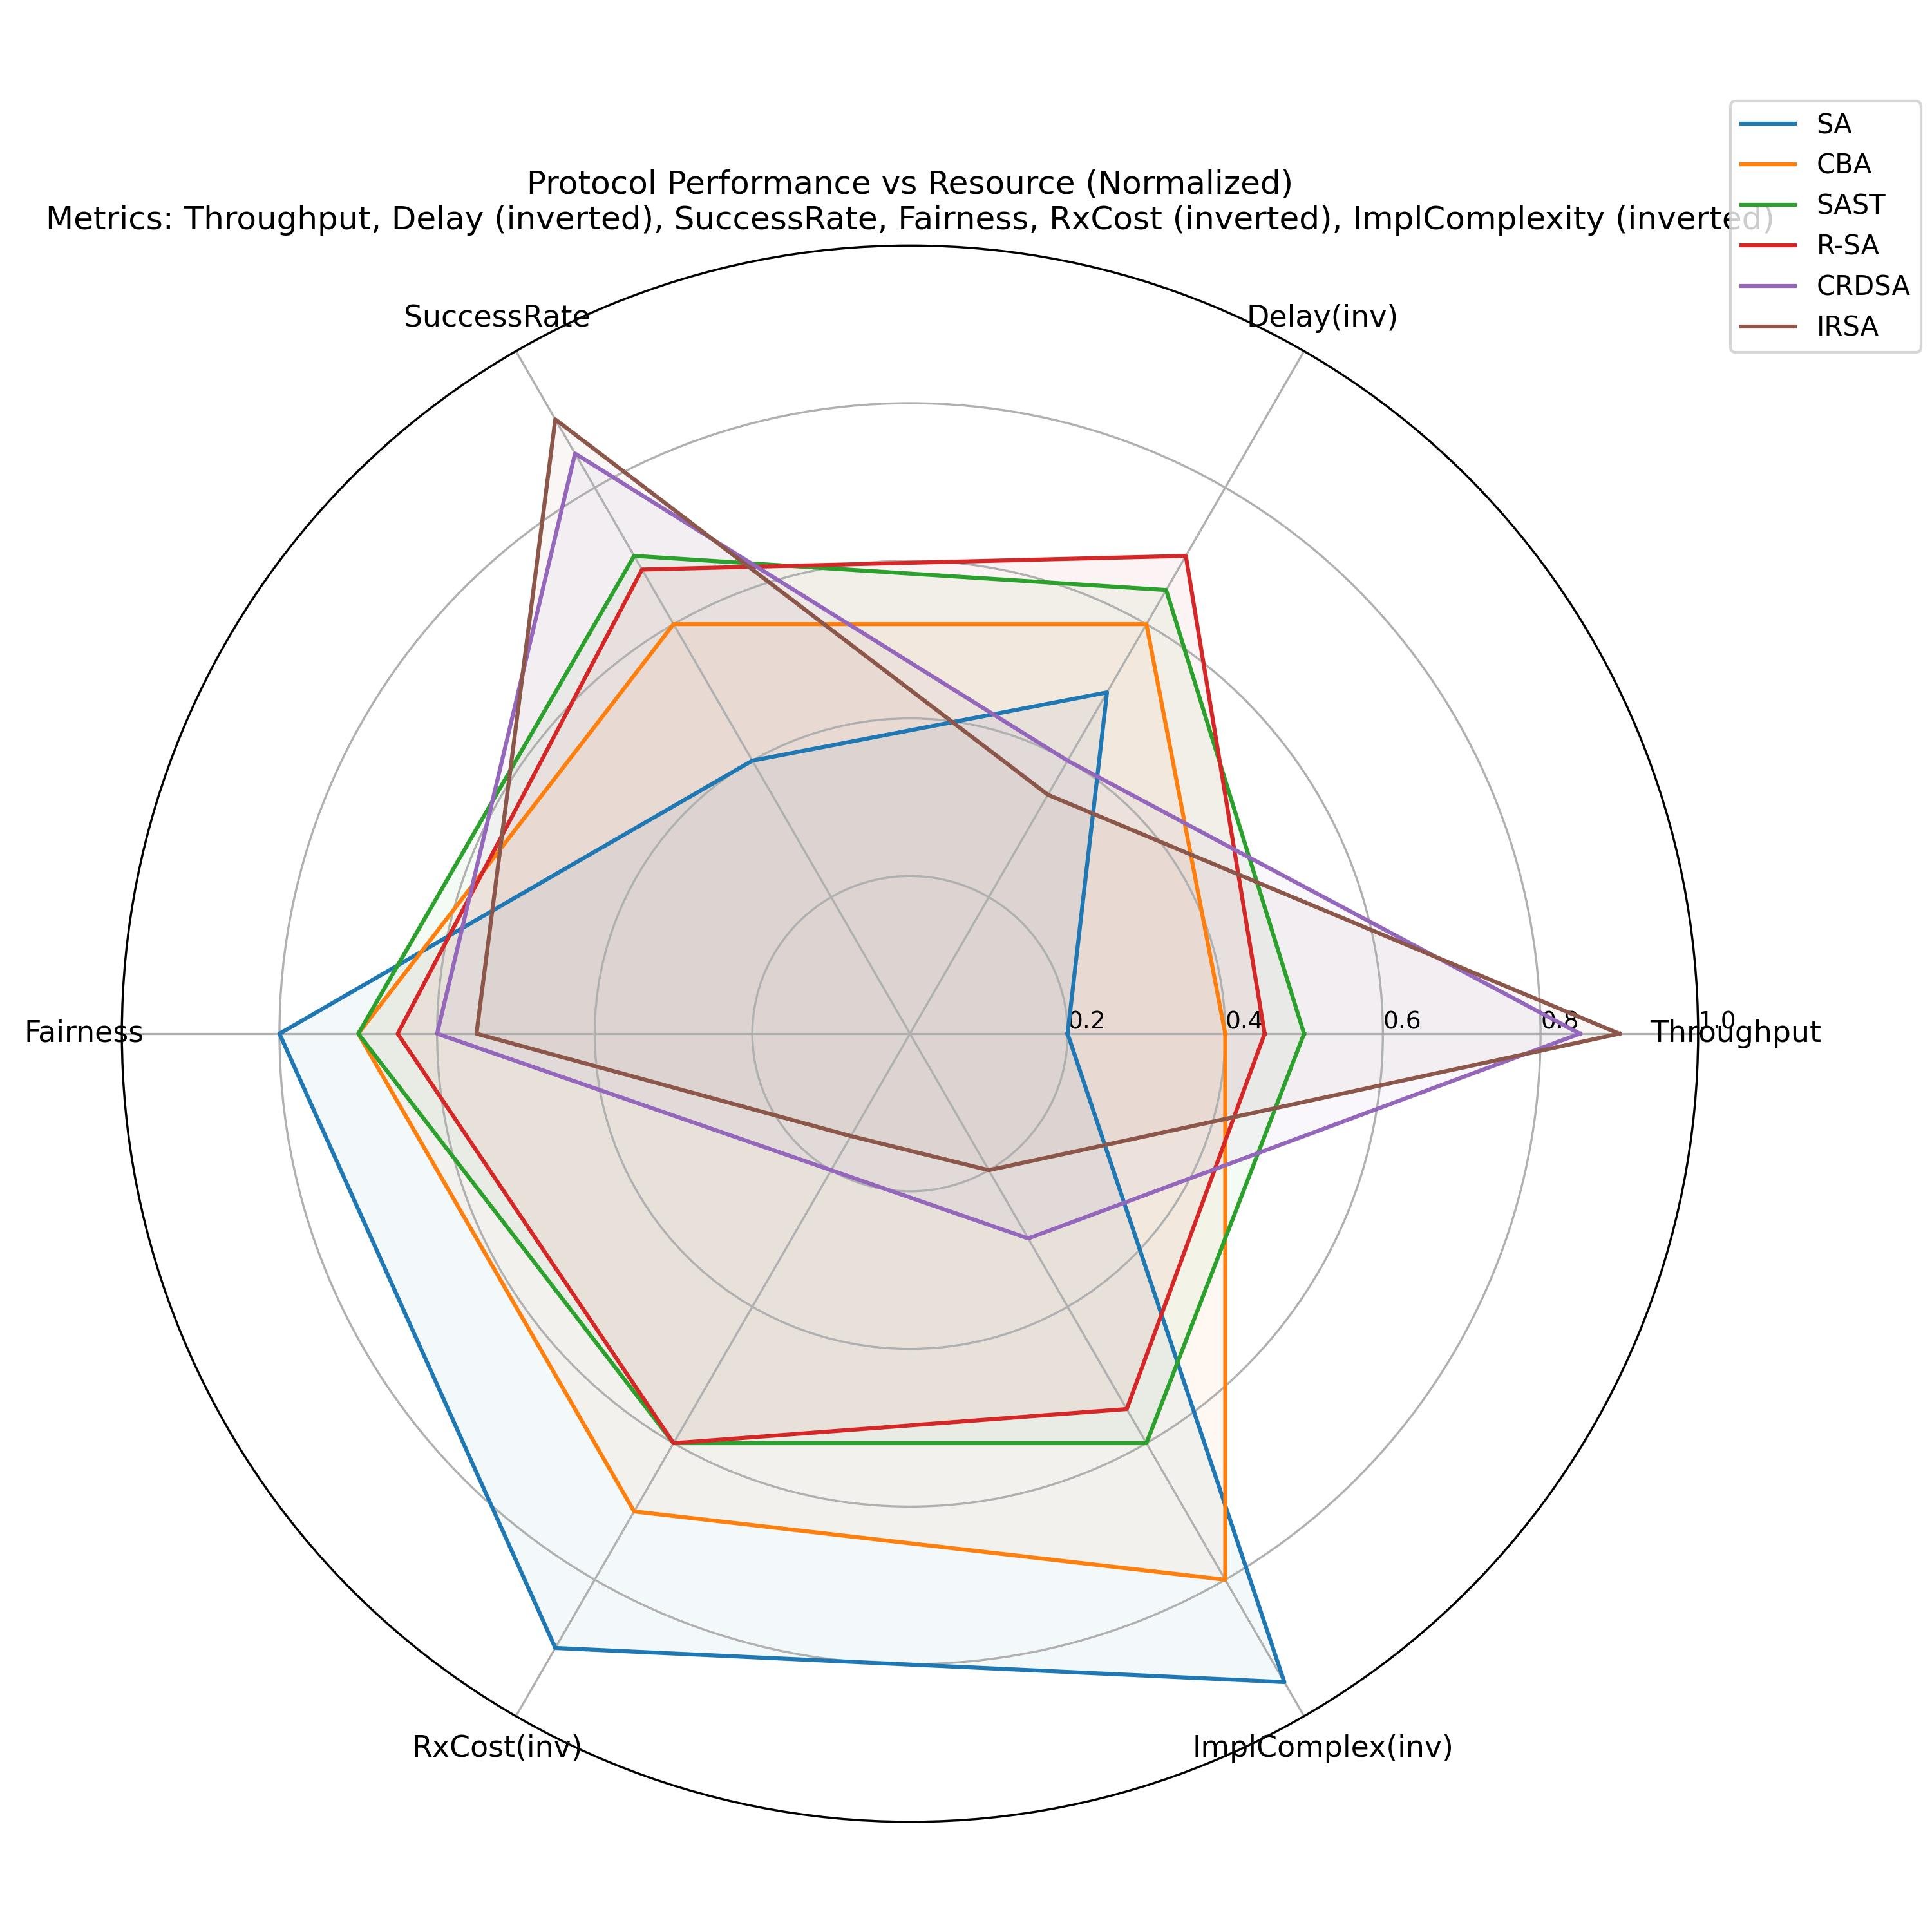
\includegraphics[width=0.3\textwidth]{figure/chap5/Sim33.jpg}
% 		\label{fig:protocol_fairness_comparison3}
% 	}
% 	\caption{不同协议在传输概率变化下的公平性对比（固定平均到达率为 $\hat{\lambda}=0.3$）。}
% 	\label{fig:protocol_fairness_comparison}
% \end{figure}


% \textbf{综合效用评估。} 
% 本小节采用综合效用 $U(\tilde{\mathbf{y}})$ 的效用权重设置为 $w_{\lambda}=0.4$、$w_D=0.3$、$w_J=0.2$、$w_S=0.1$。图~\ref{fig:protocol_utility_comparison} 展示了基于式~\eqref{eq:chap5_constrained} 定义的综合效用 $U(\tilde{\mathbf{y}})$ 对比结果。

% \begin{figure}[t]
% 	\centering
% 	\subfloat[均匀场景]{
% 		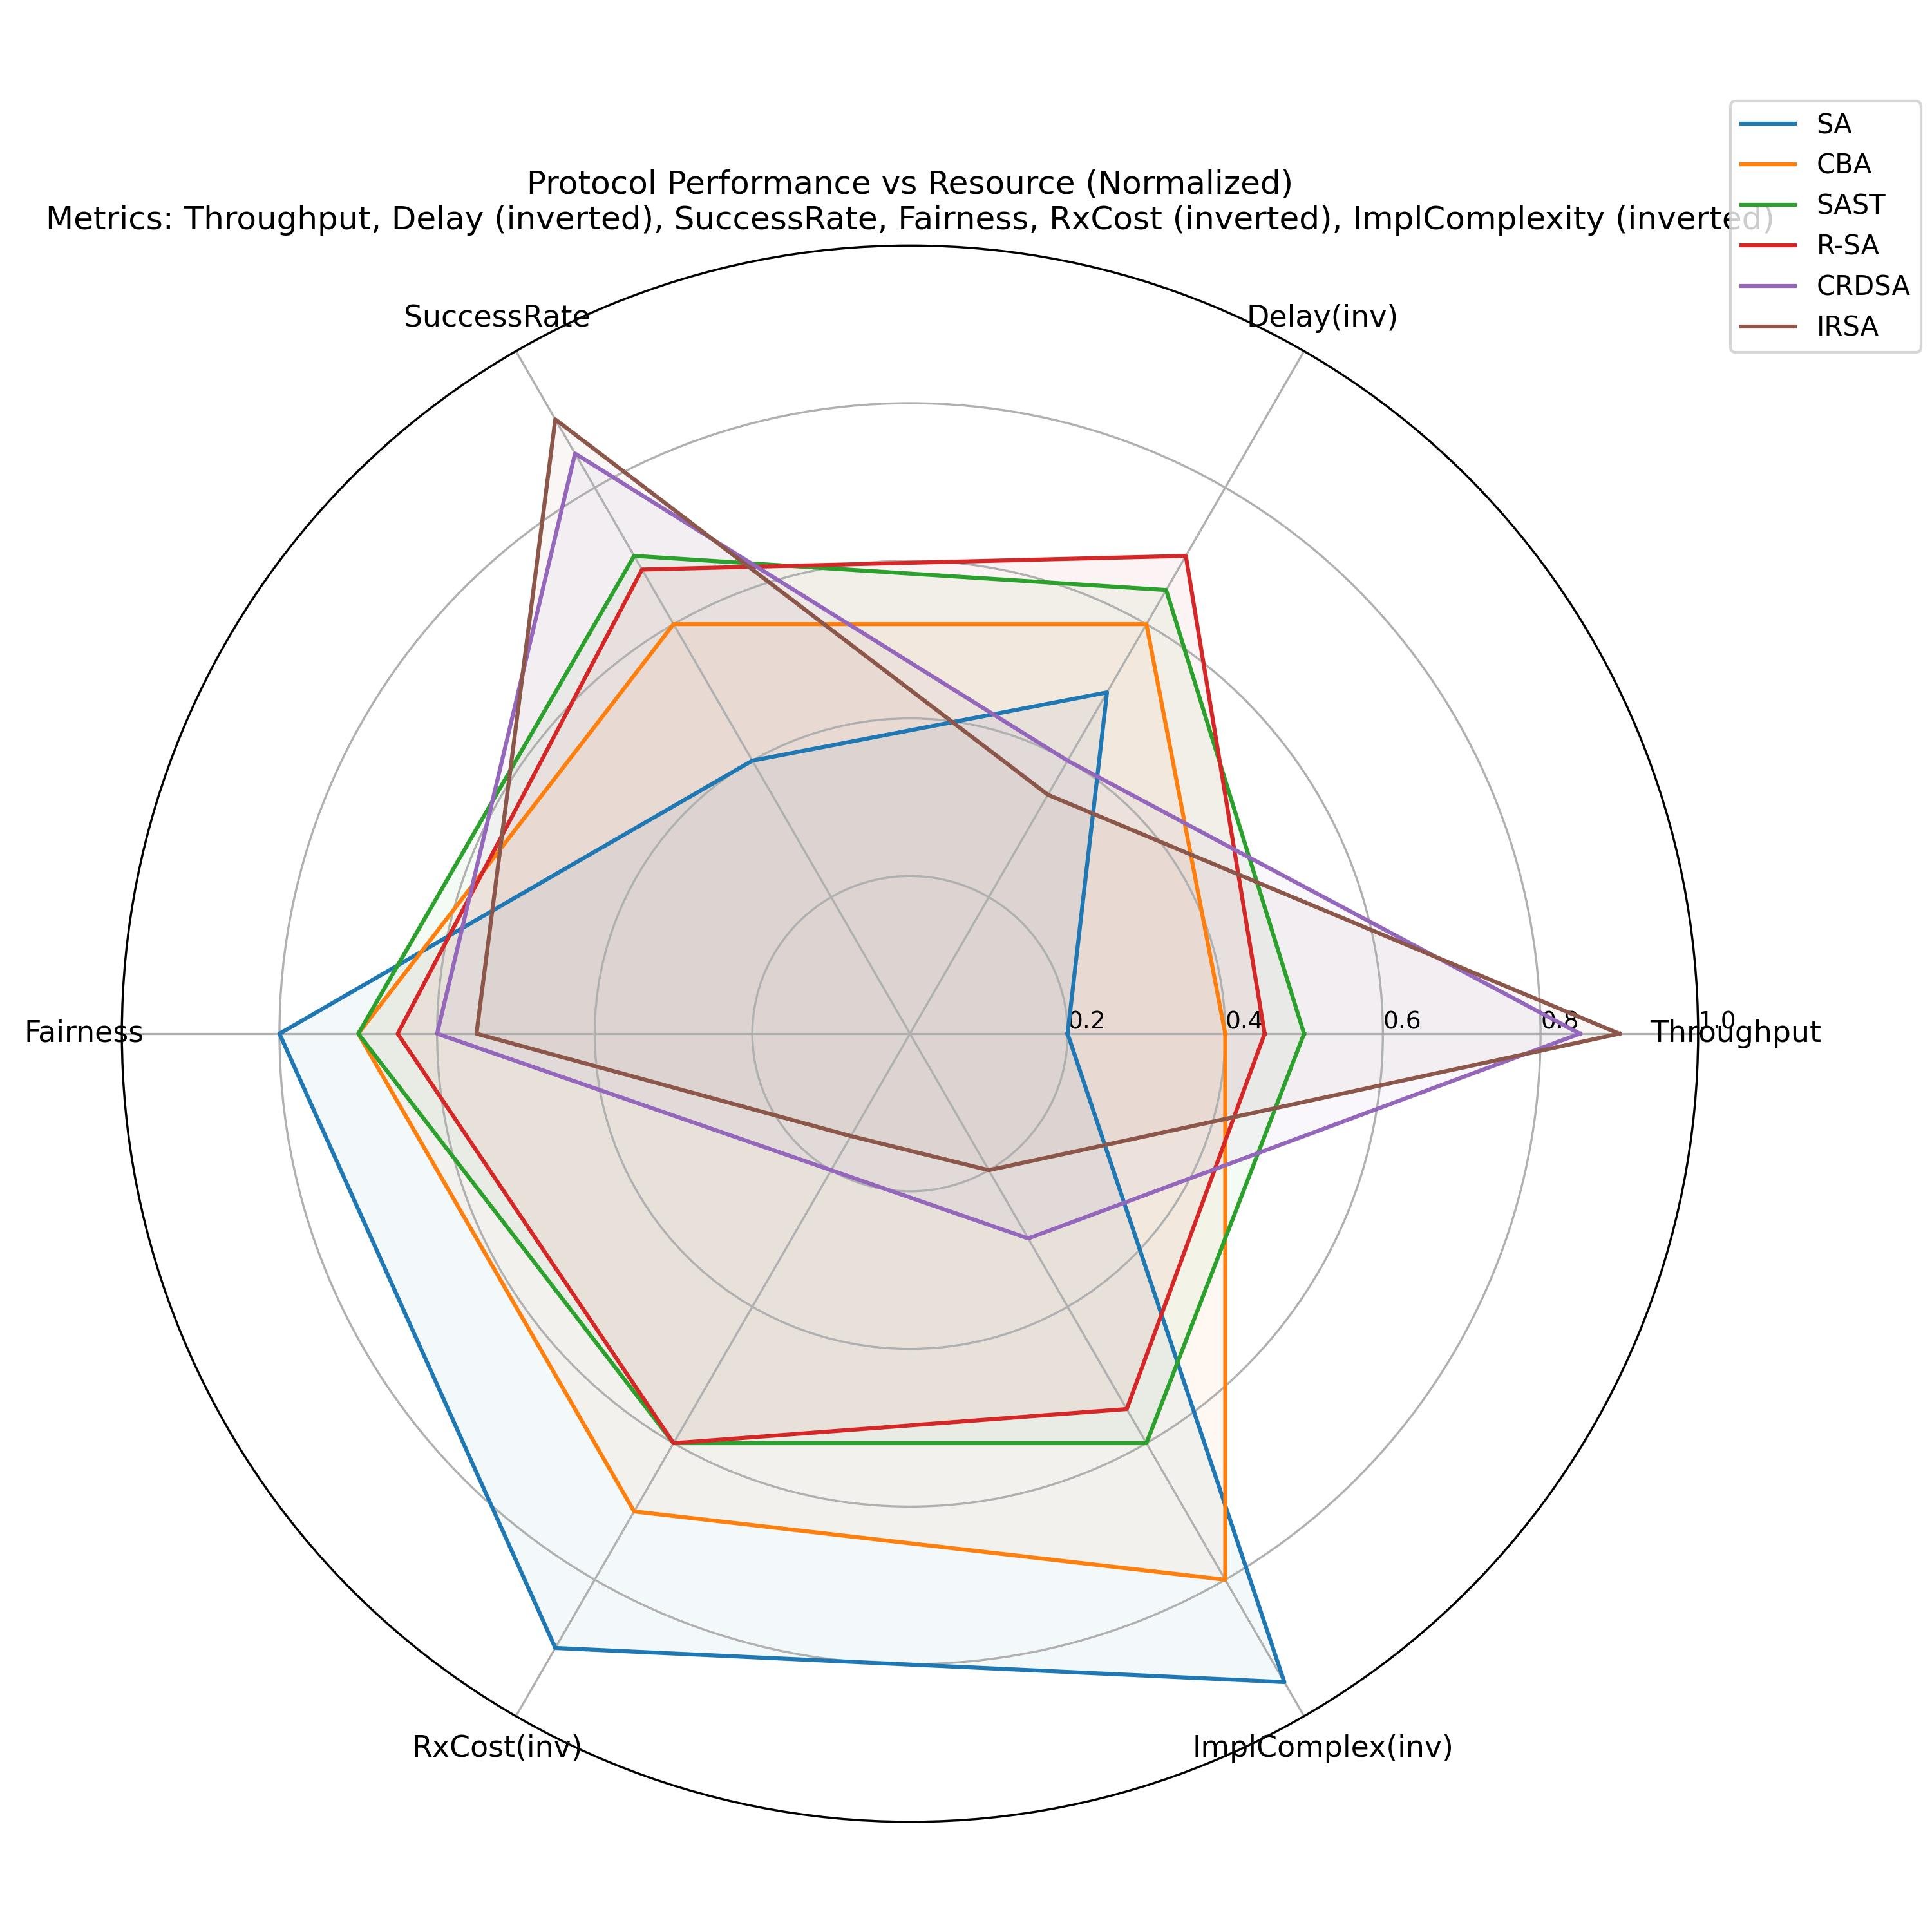
\includegraphics[width=0.3\textwidth]{figure/chap5/Sim41.jpg}
% 		\label{fig:protocol_utility_comparison1}
% 	}
% 	\hfill
% 	\subfloat[突发场景]{
% 		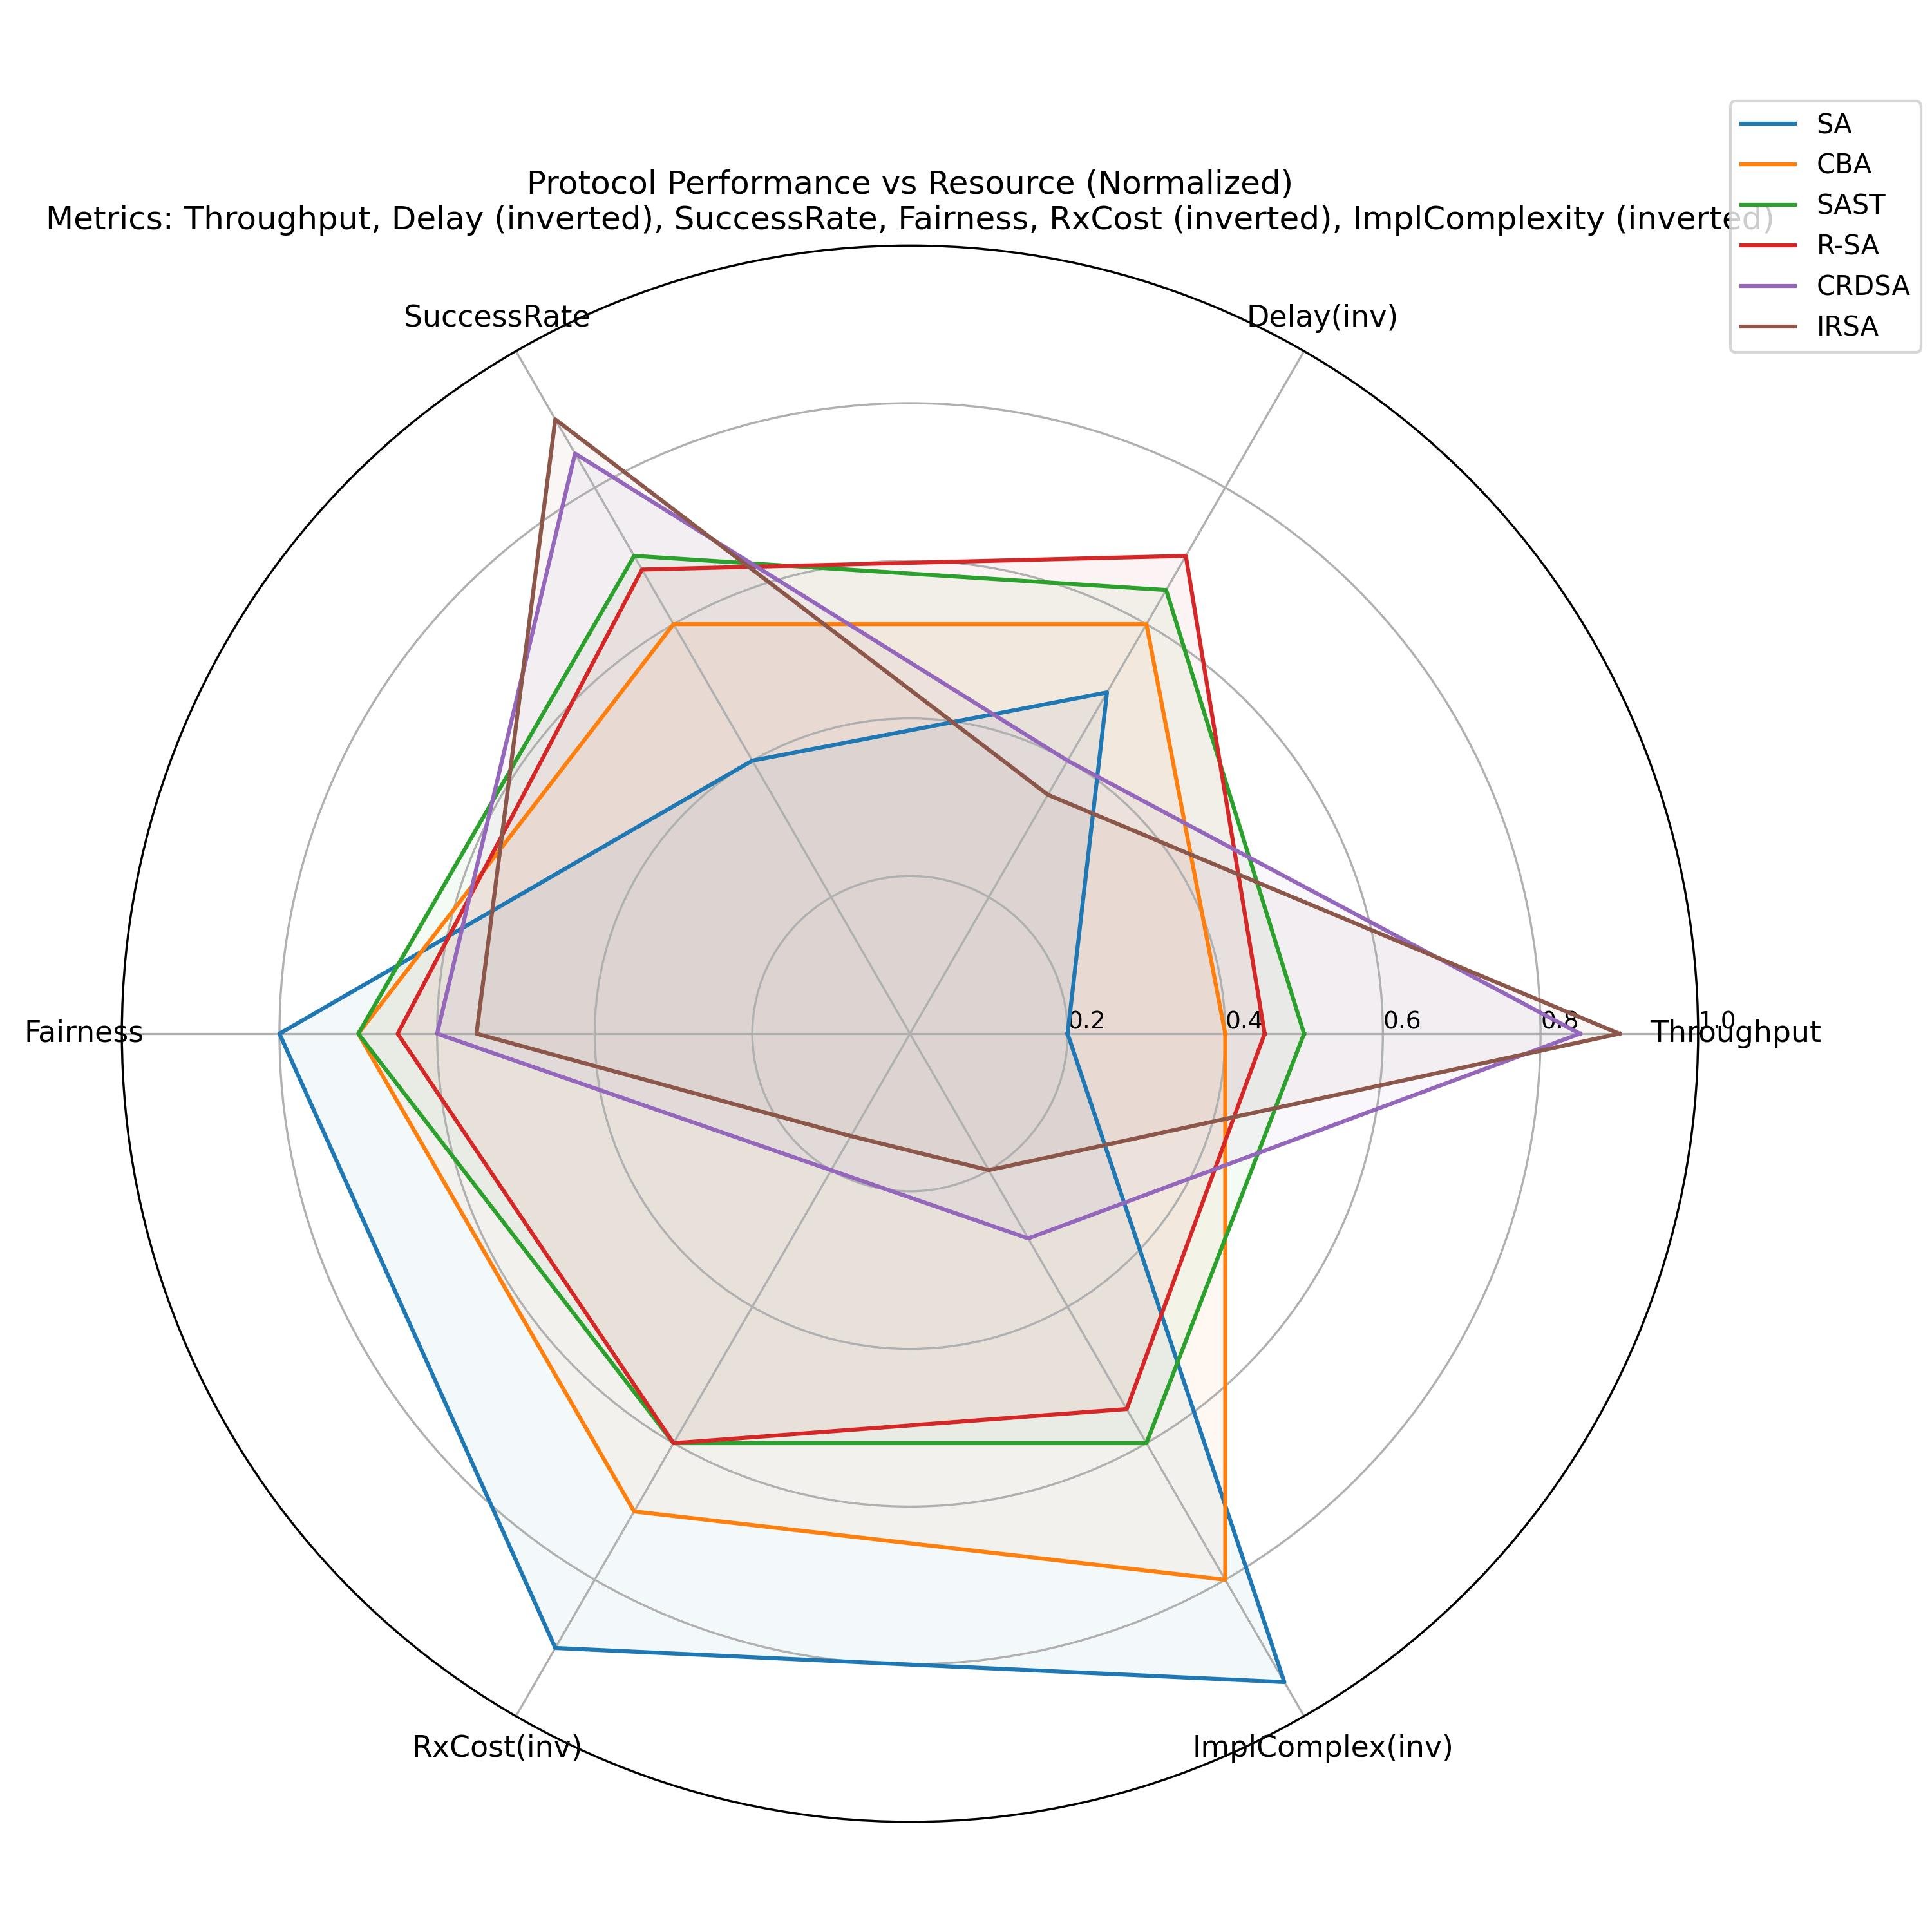
\includegraphics[width=0.3\textwidth]{figure/chap5/Sim42.jpg}
% 		\label{fig:protocol_utility_comparison2}
% 	}
% 	\hfill
% 	\subfloat[周期场景]{
% 		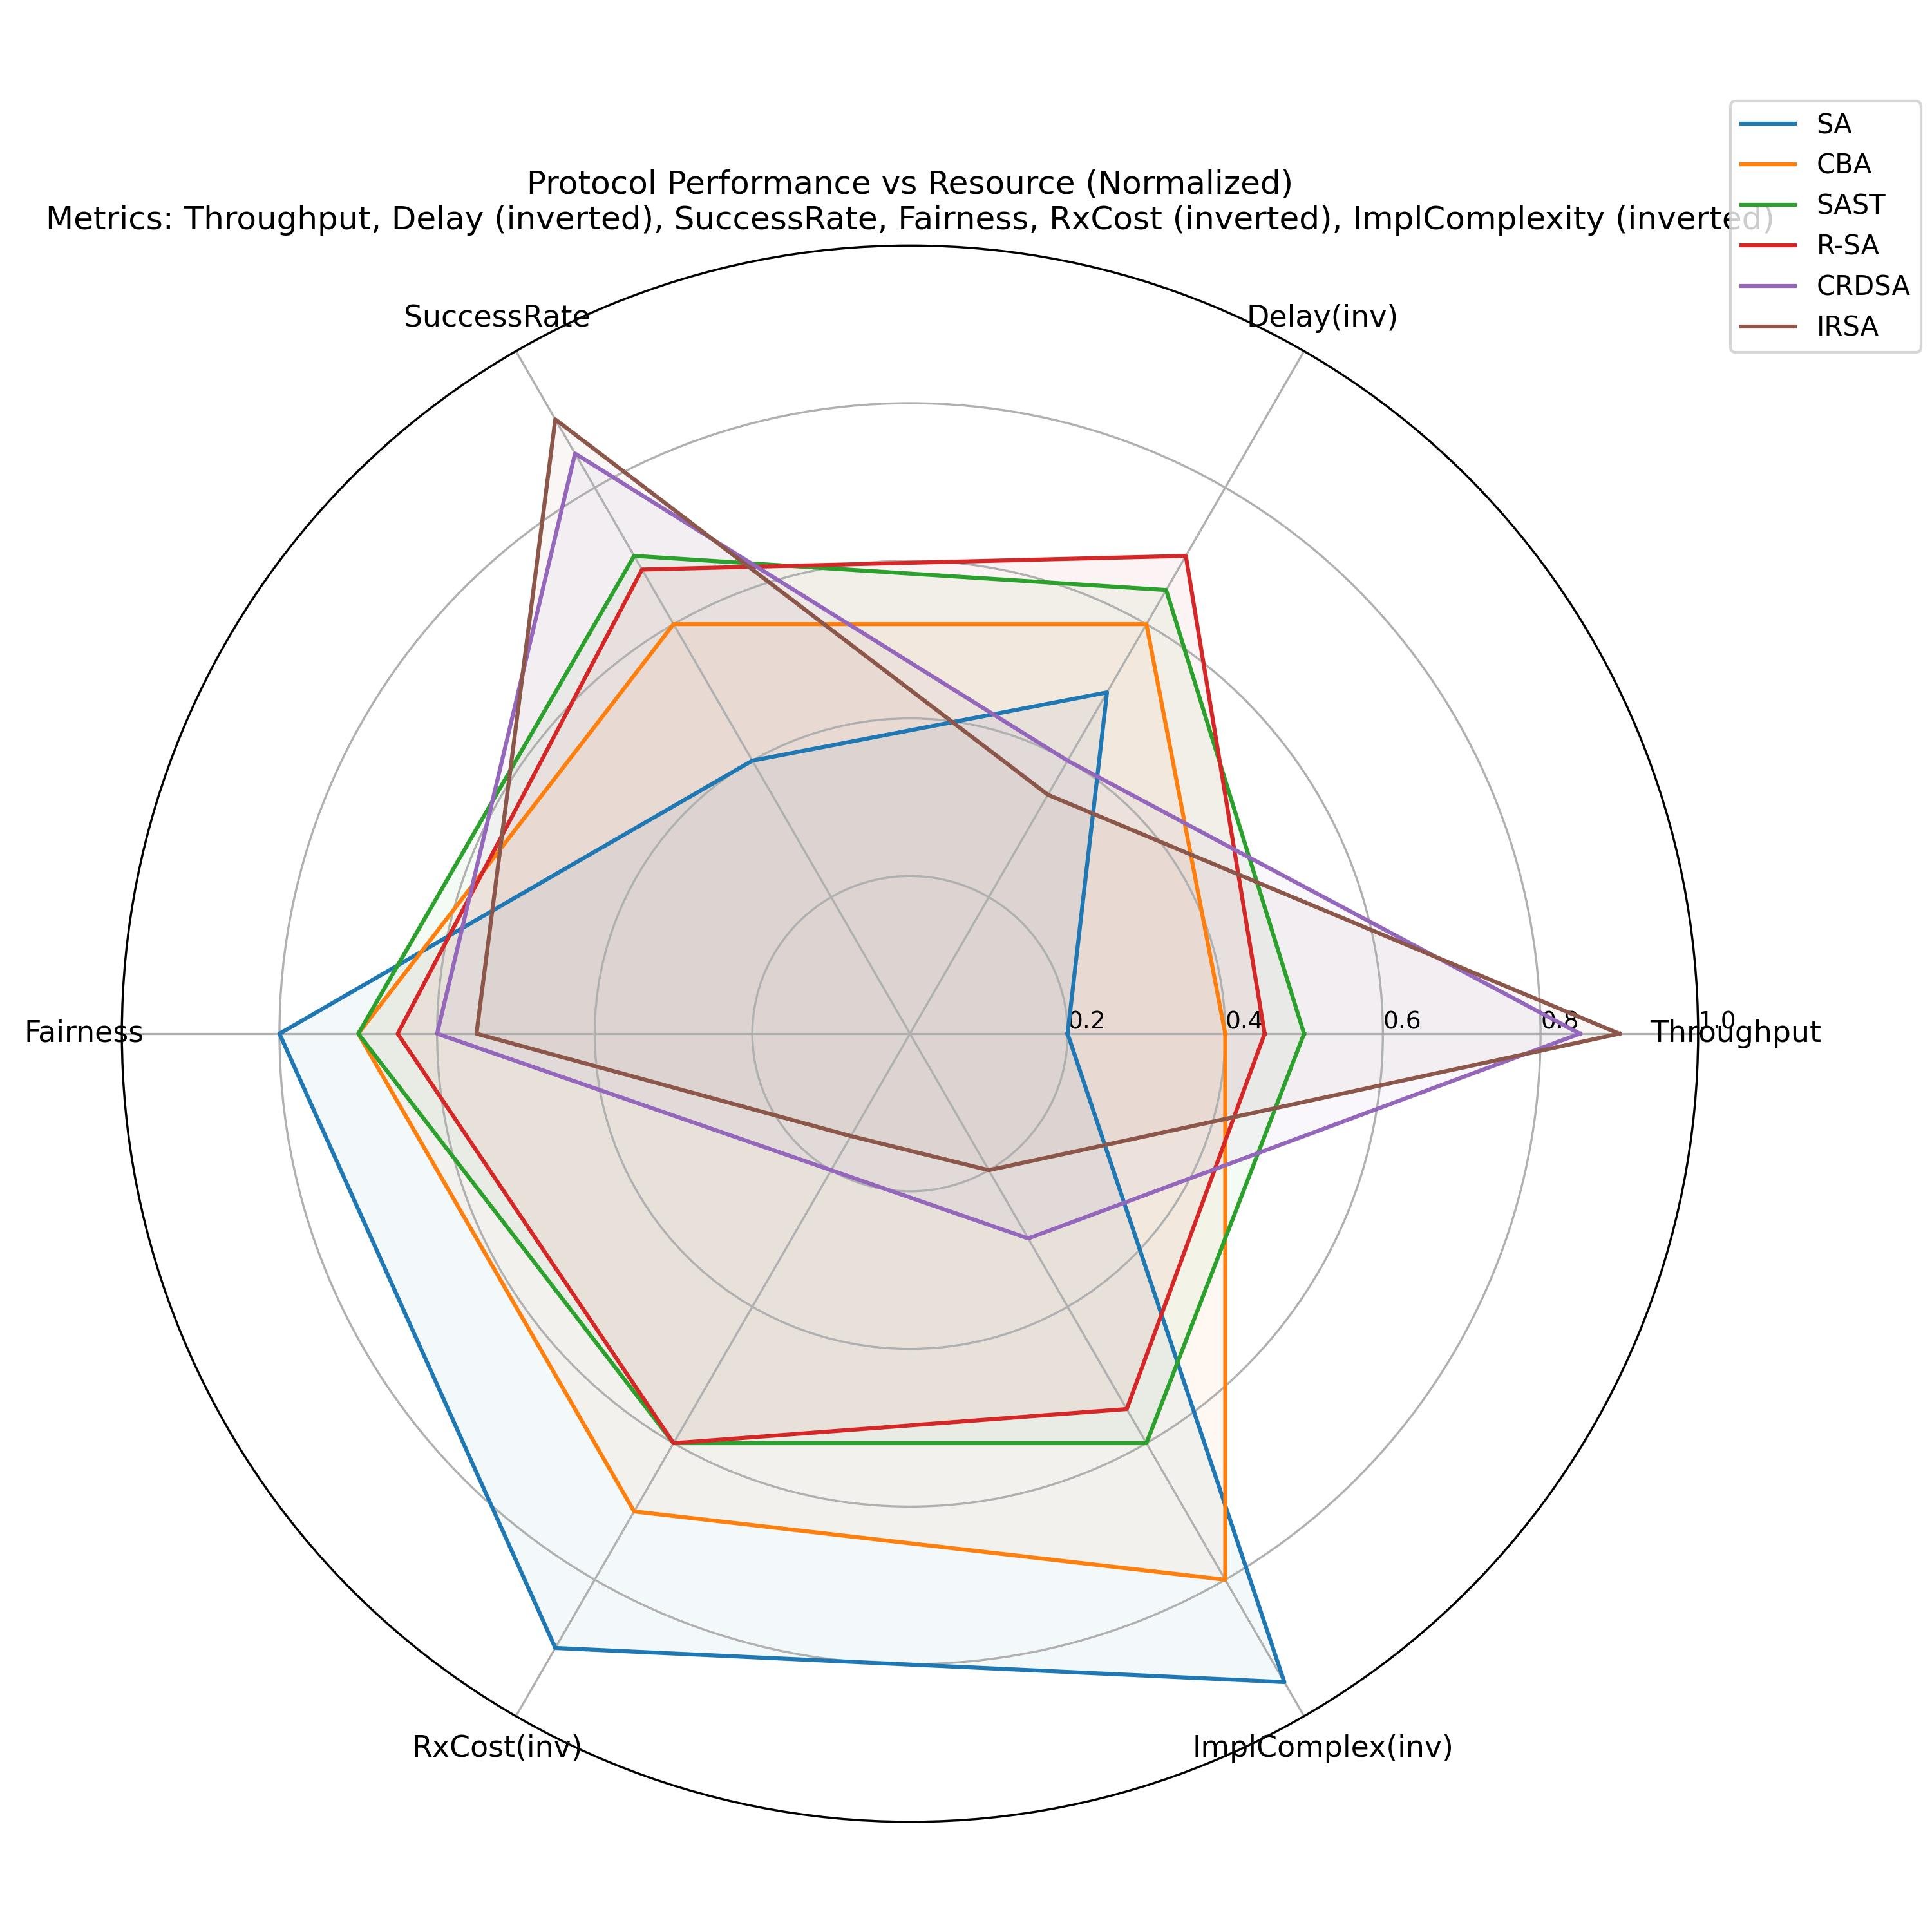
\includegraphics[width=0.3\textwidth]{figure/chap5/Sim43.jpg}
% 		\label{fig:protocol_utility_comparison3}
% 	}
% 	\caption{不同协议在传输概率变化下的综合效用对比（固定平均到达率为 $\hat{\lambda}=0.3$）。}
% 	\label{fig:protocol_utility_comparison}
% \end{figure}

% === 1. 将下列内容剪切到5.2.4节合适位置（如“仿真性能验证与对比”小节中） ===

% \subsection{不同\(\lambda\)下均匀流量场景的性能对比}
% 为进一步展示不同协议在均匀流量（uniform）场景下随接入概率\(q\)变化的性能差异，本文对\(\lambda=0.001, 0.003, 0.005, 0.01\)四种典型到达率下的时延、吞吐量、公平性、信令开销等指标进行了仿真对比，结果如下图所示。

% % 延迟对比
% \begin{figure}[htbp]
%     \centering
%     % 四个子图
%     \subfloat[$\lambda=0.01$]{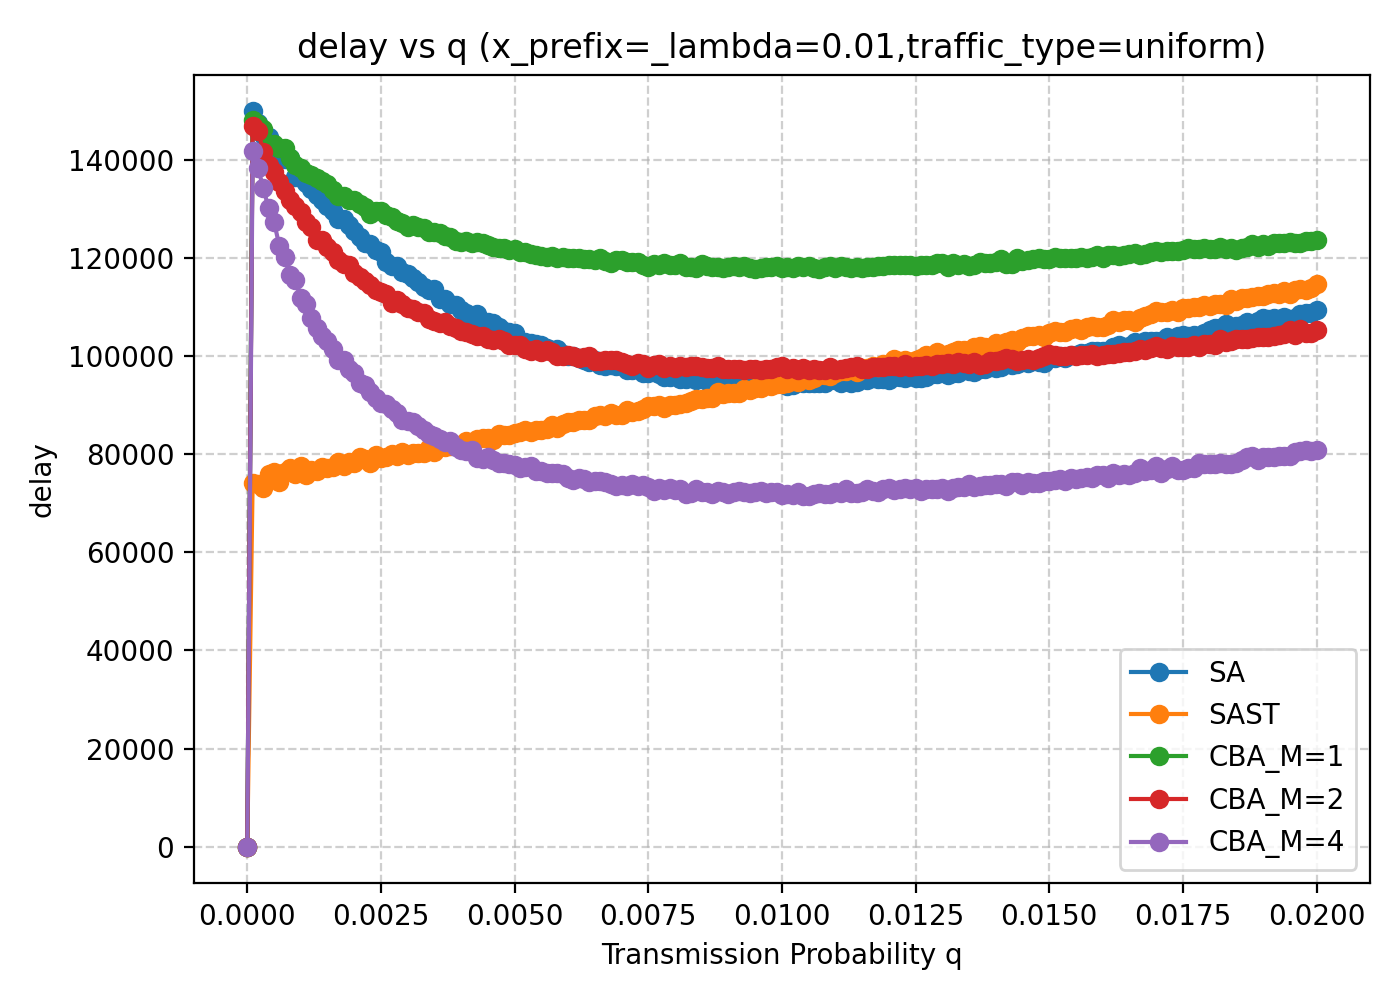
\includegraphics[width=0.24\textwidth]{figure/chap5/delay_vs_q_xprefix__lambda=0.01,traffic_type=uniform.pdf}}
%     \subfloat[$\lambda=0.001$]{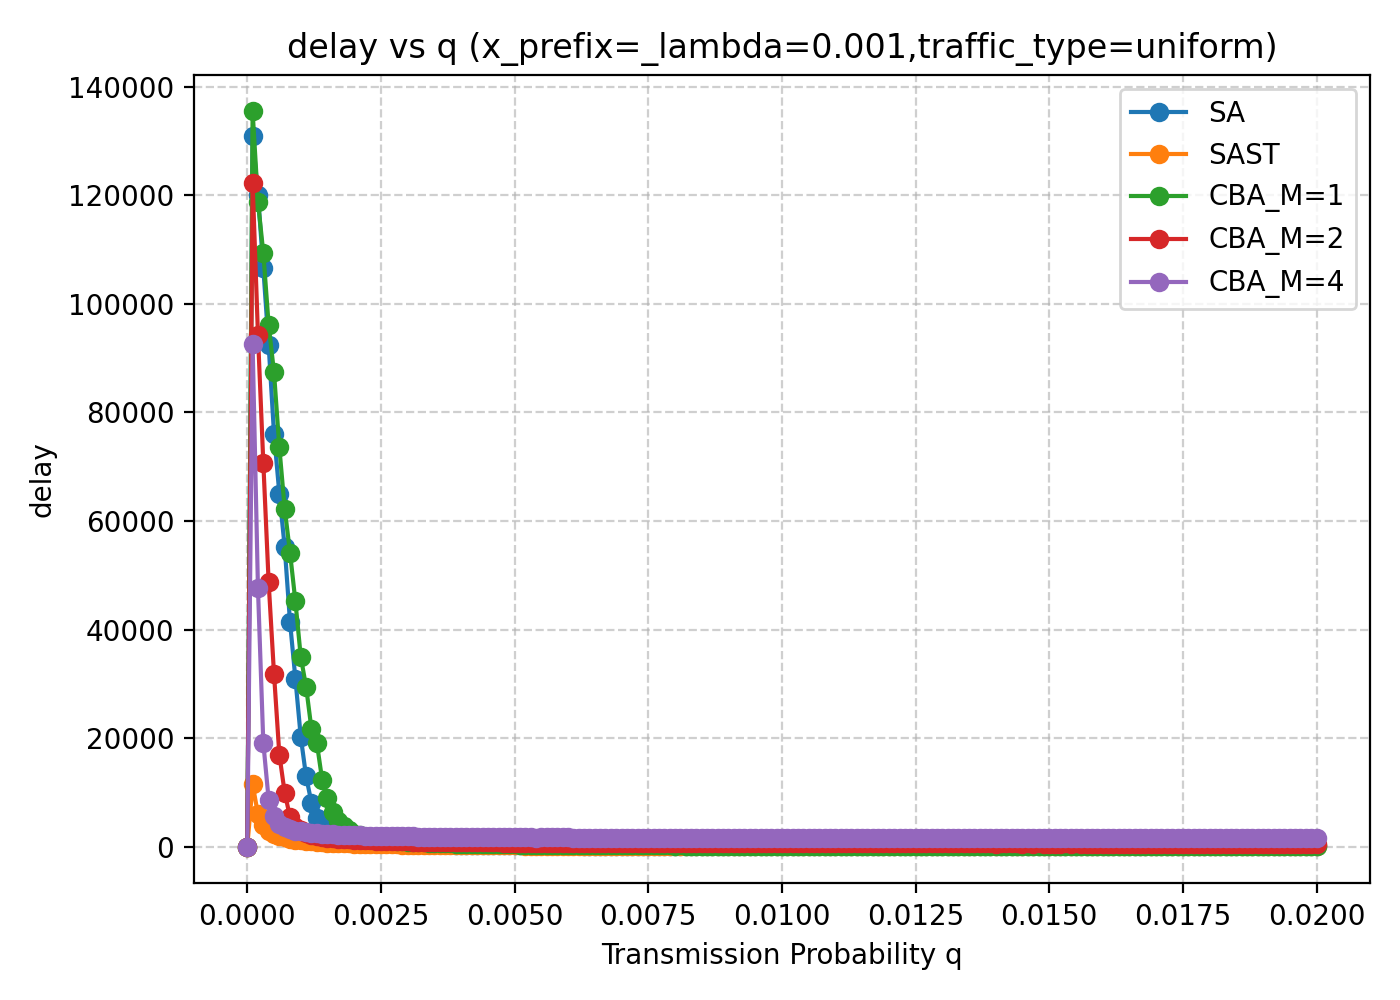
\includegraphics[width=0.24\textwidth]{figure/chap5/delay_vs_q_xprefix__lambda=0.001,traffic_type=uniform.pdf}}
%     \subfloat[$\lambda=0.003$]{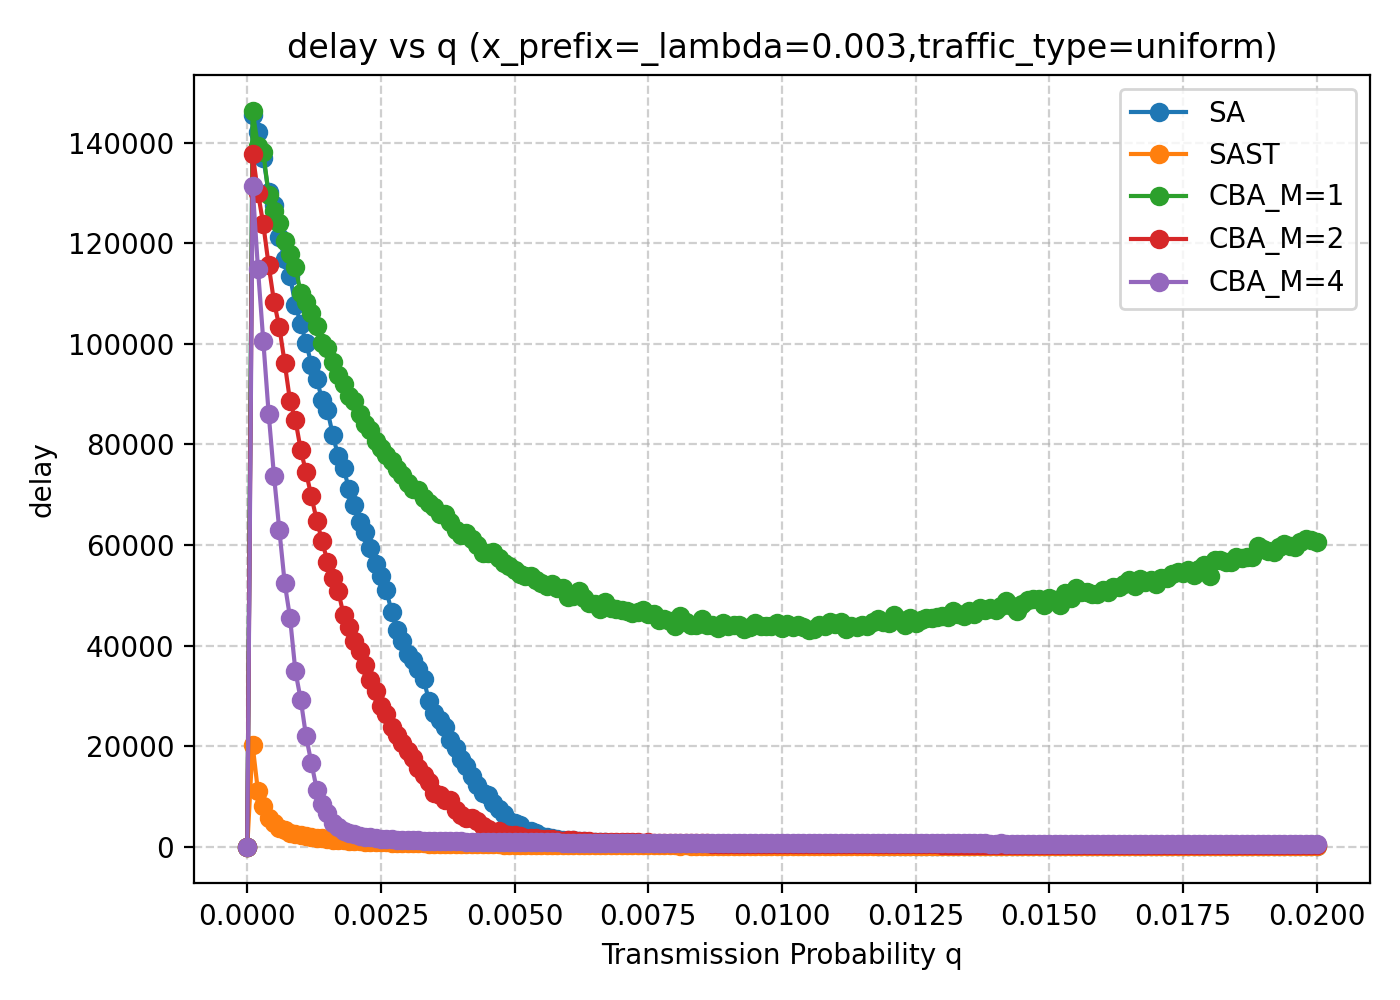
\includegraphics[width=0.24\textwidth]{figure/chap5/delay_vs_q_xprefix__lambda=0.003,traffic_type=uniform.pdf}}
%     \subfloat[$\lambda=0.005$]{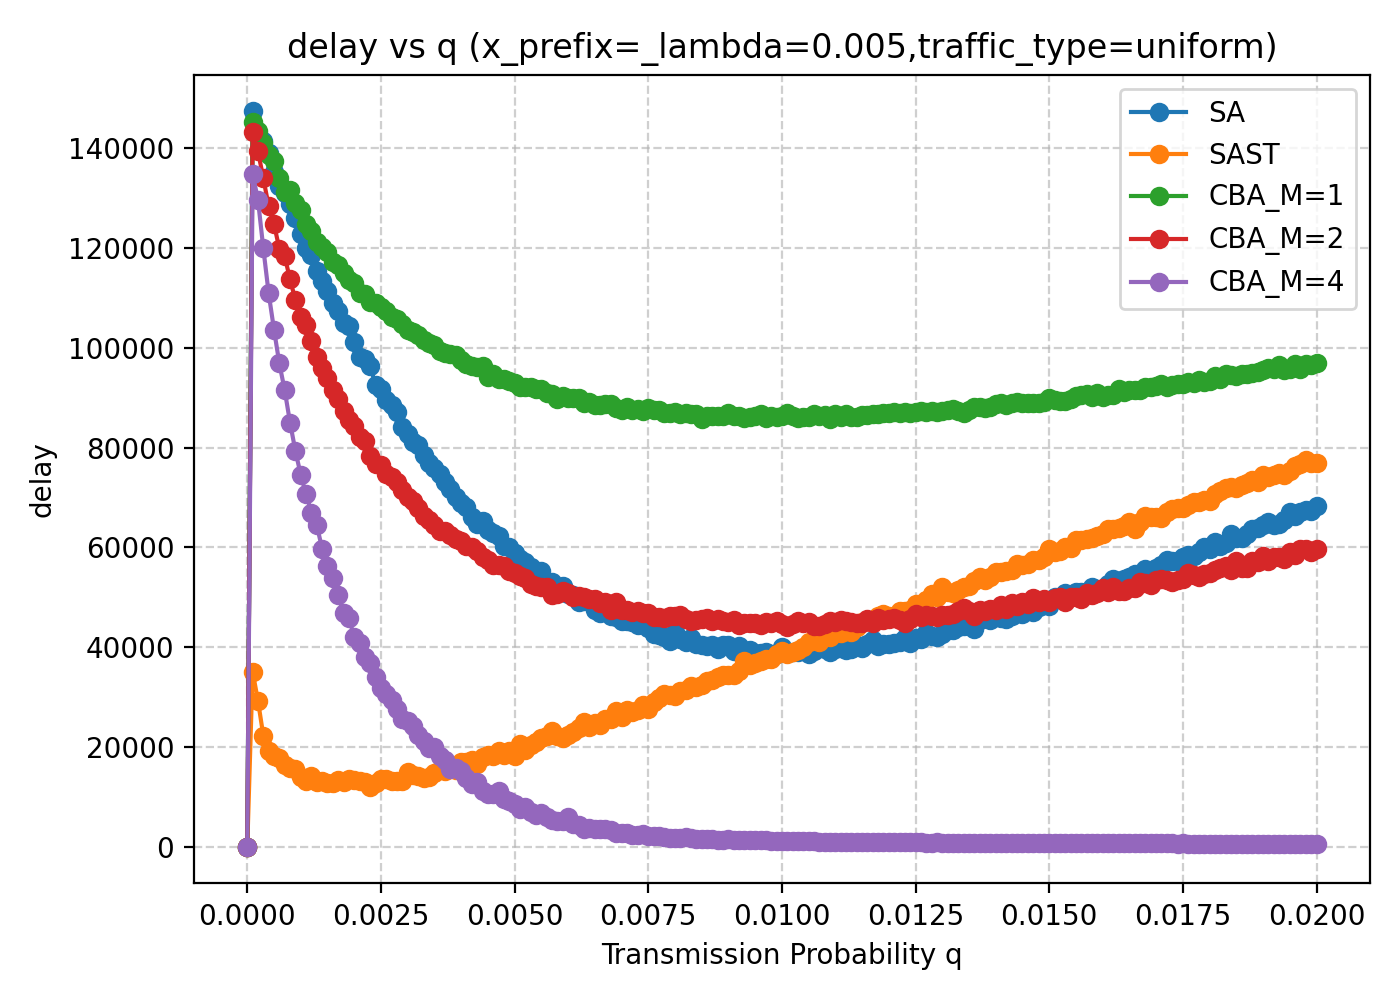
\includegraphics[width=0.24\textwidth]{figure/chap5/delay_vs_q_xprefix__lambda=0.005,traffic_type=uniform.pdf}}
%     \caption{不同$\lambda$下均匀流量场景的平均时延$D$随$q$变化对比}
%     \label{fig:delay_vs_q_uniform}
% \end{figure}

% % 公平性对比
% \begin{figure}[htbp]
%     \centering
%     \subfloat[$\lambda=0.01$]{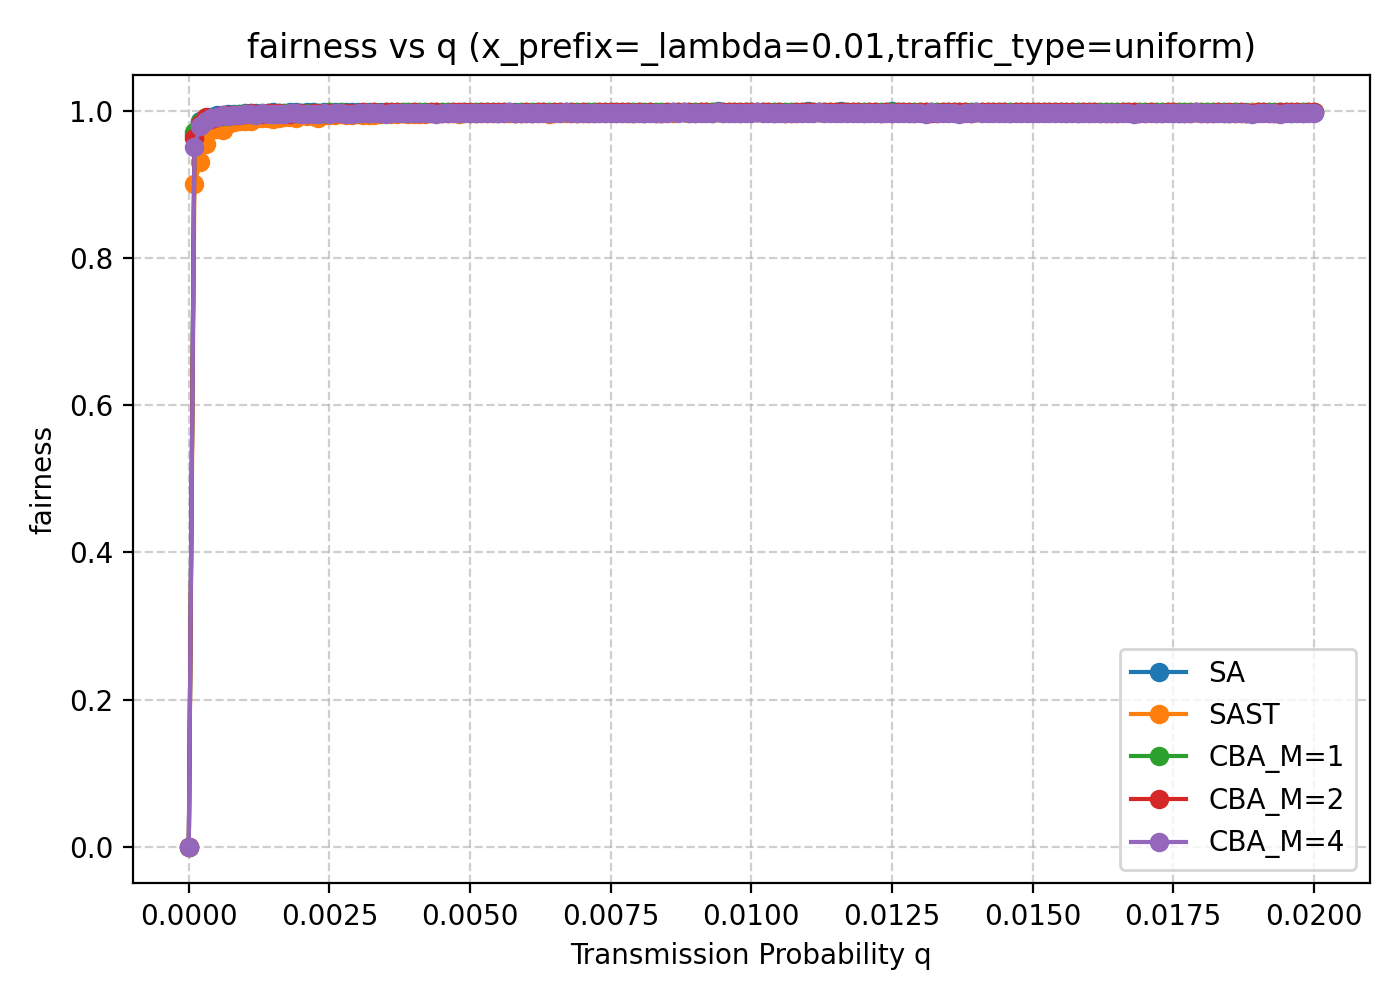
\includegraphics[width=0.24\textwidth]{figure/chap5/fairness_vs_q_xprefix__lambda=0.01,traffic_type=uniform.pdf}}
%     \subfloat[$\lambda=0.001$]{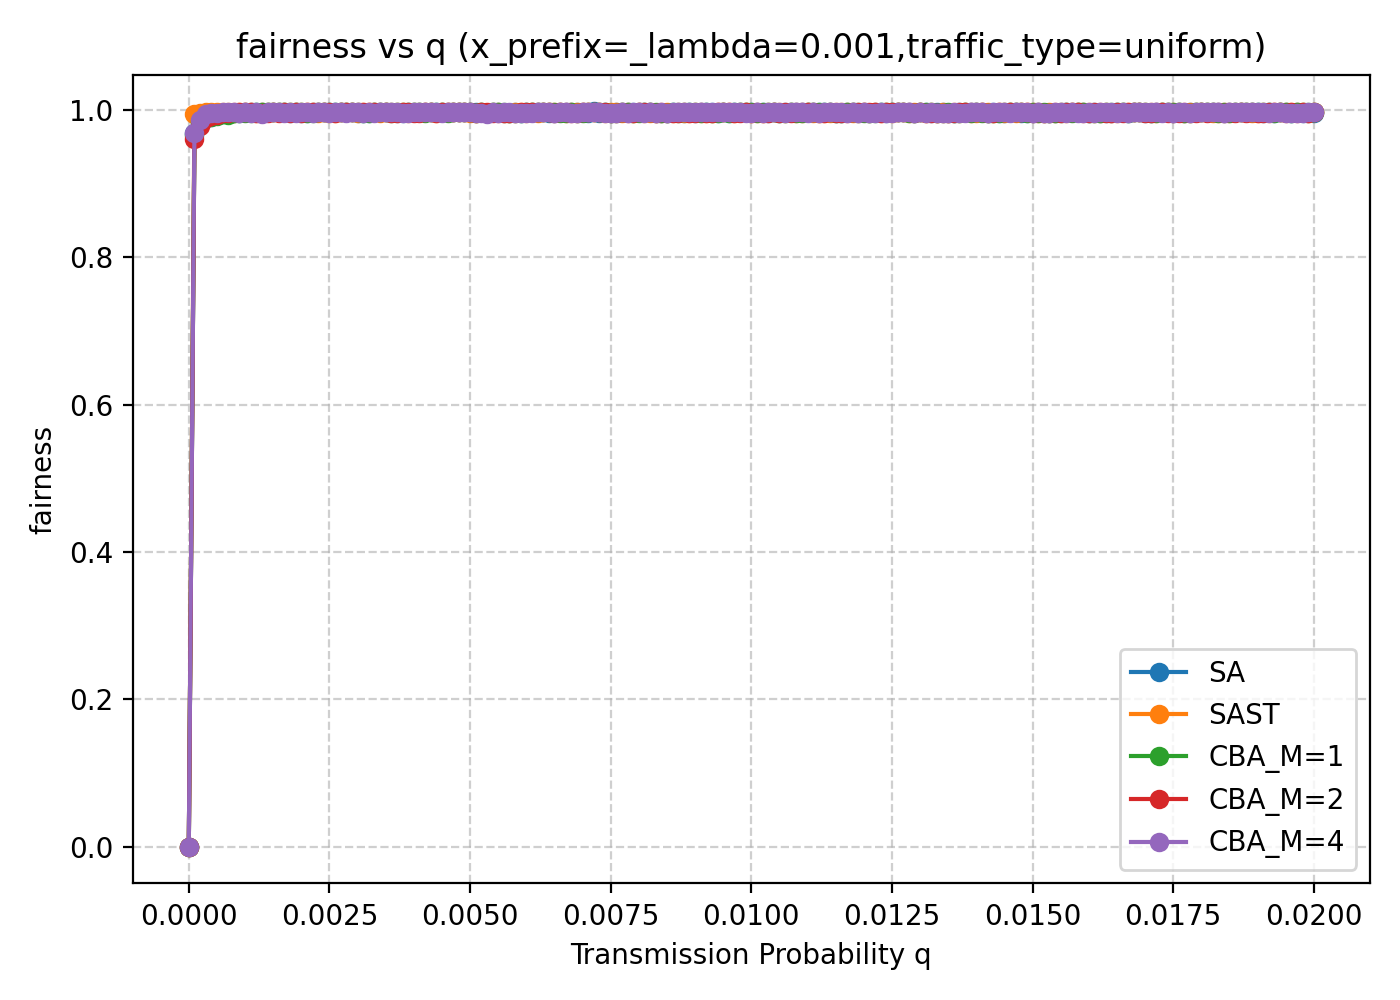
\includegraphics[width=0.24\textwidth]{figure/chap5/fairness_vs_q_xprefix__lambda=0.001,traffic_type=uniform.pdf}}
%     \subfloat[$\lambda=0.003$]{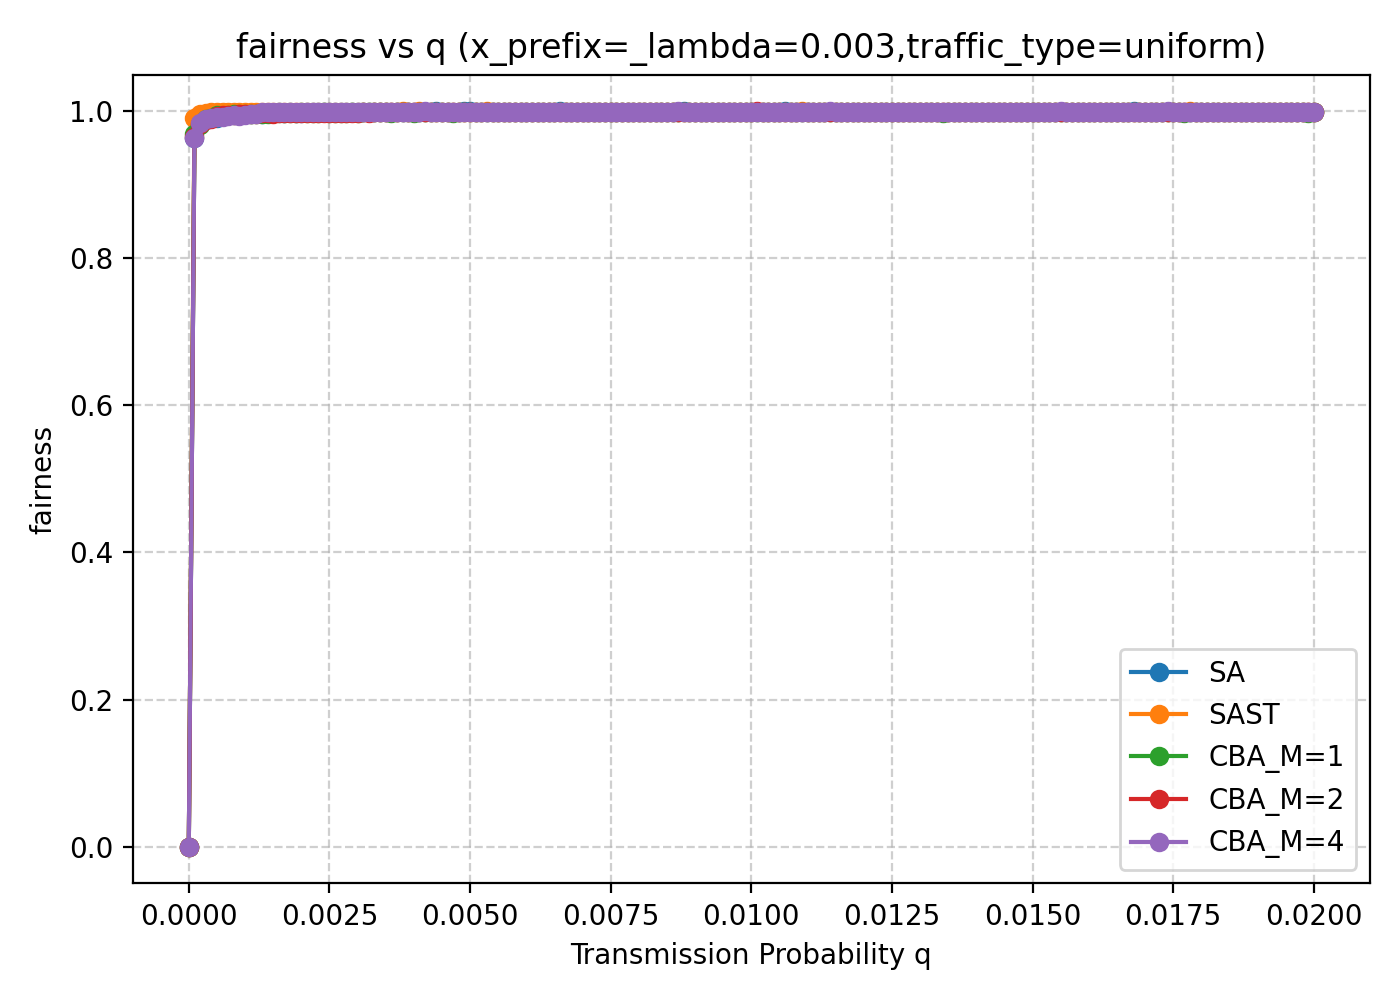
\includegraphics[width=0.24\textwidth]{figure/chap5/fairness_vs_q_xprefix__lambda=0.003,traffic_type=uniform.pdf}}
%     \subfloat[$\lambda=0.005$]{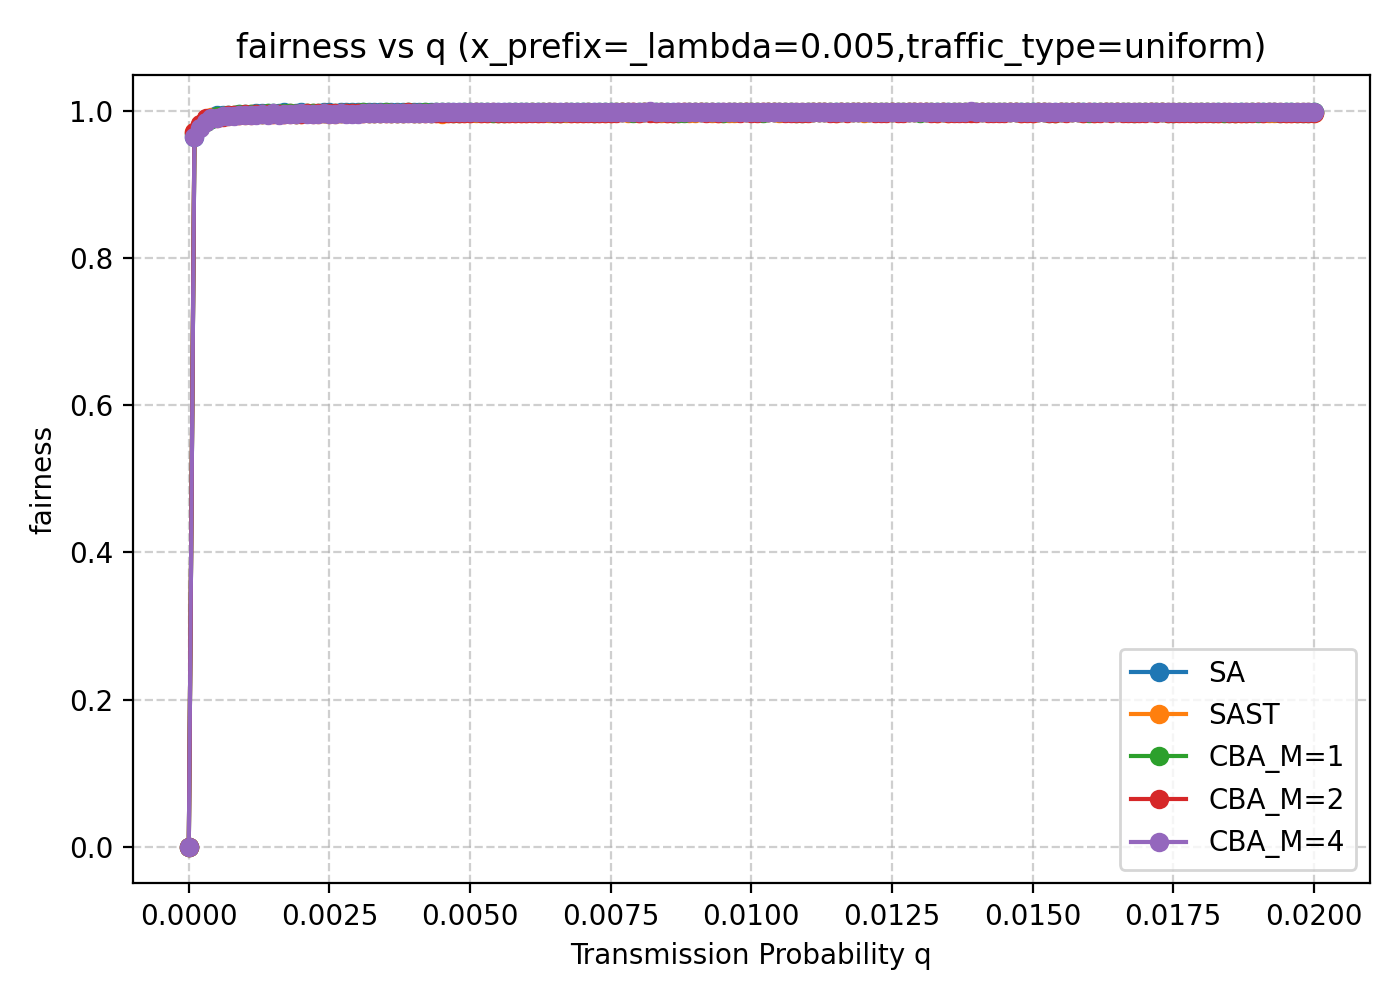
\includegraphics[width=0.24\textwidth]{figure/chap5/fairness_vs_q_xprefix__lambda=0.005,traffic_type=uniform.pdf}}
%     \caption{不同$\lambda$下均匀流量场景的公平性$J_T$随$q$变化对比}
%     \label{fig:fairness_vs_q_uniform}
% \end{figure}

% % 信令开销对比
% \begin{figure}[htbp]
%     \centering
%     \subfloat[$\lambda=0.01$]{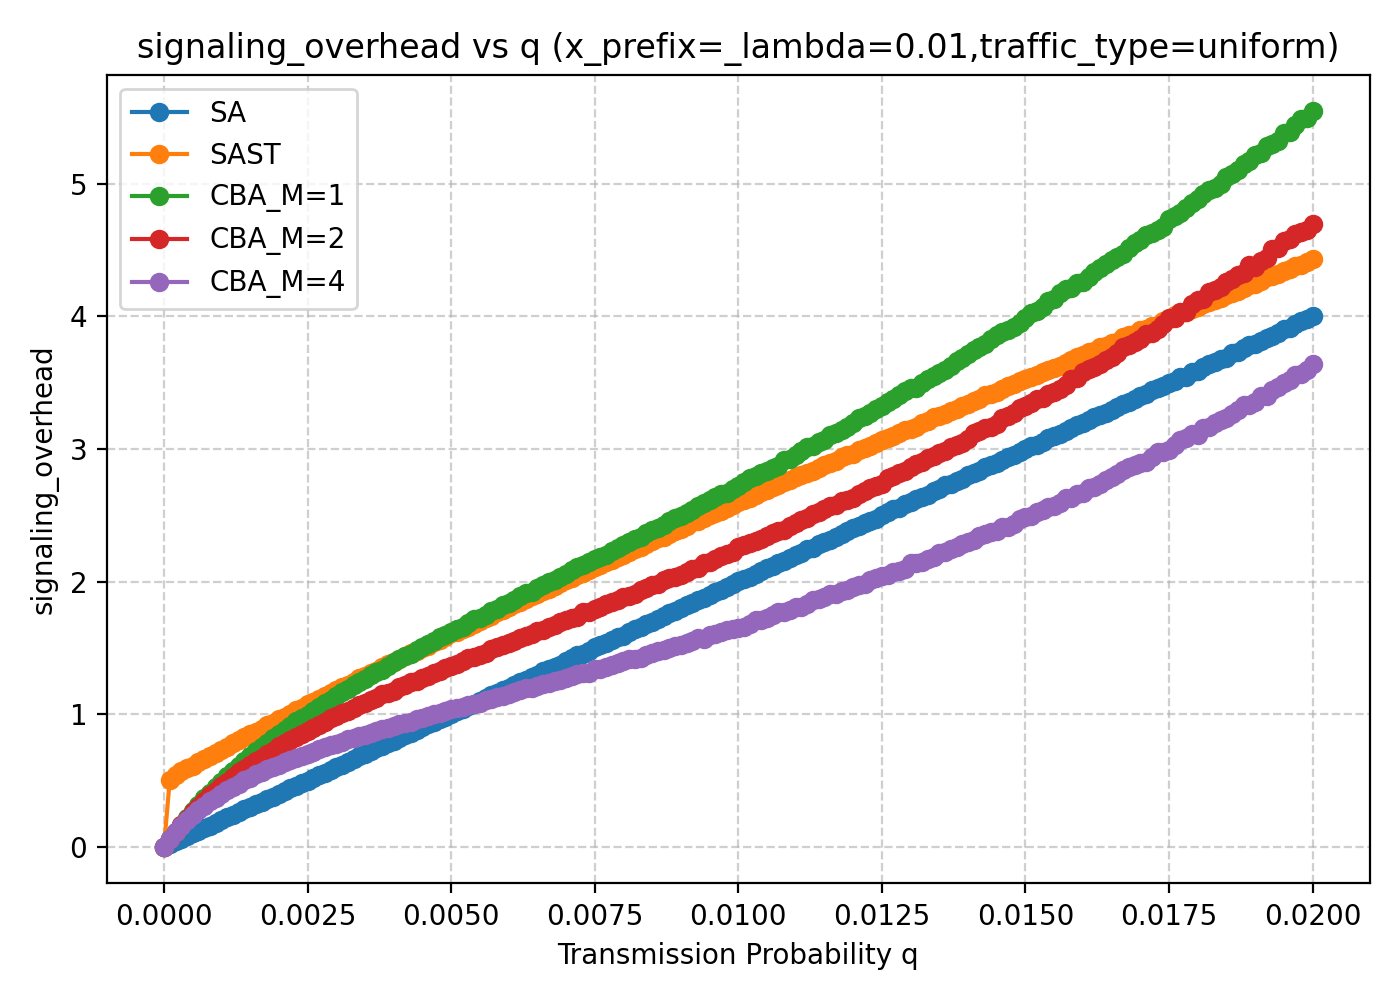
\includegraphics[width=0.24\textwidth]{figure/chap5/signaling_overhead_vs_q_xprefix__lambda=0.01,traffic_type=uniform.pdf}}
%     \subfloat[$\lambda=0.001$]{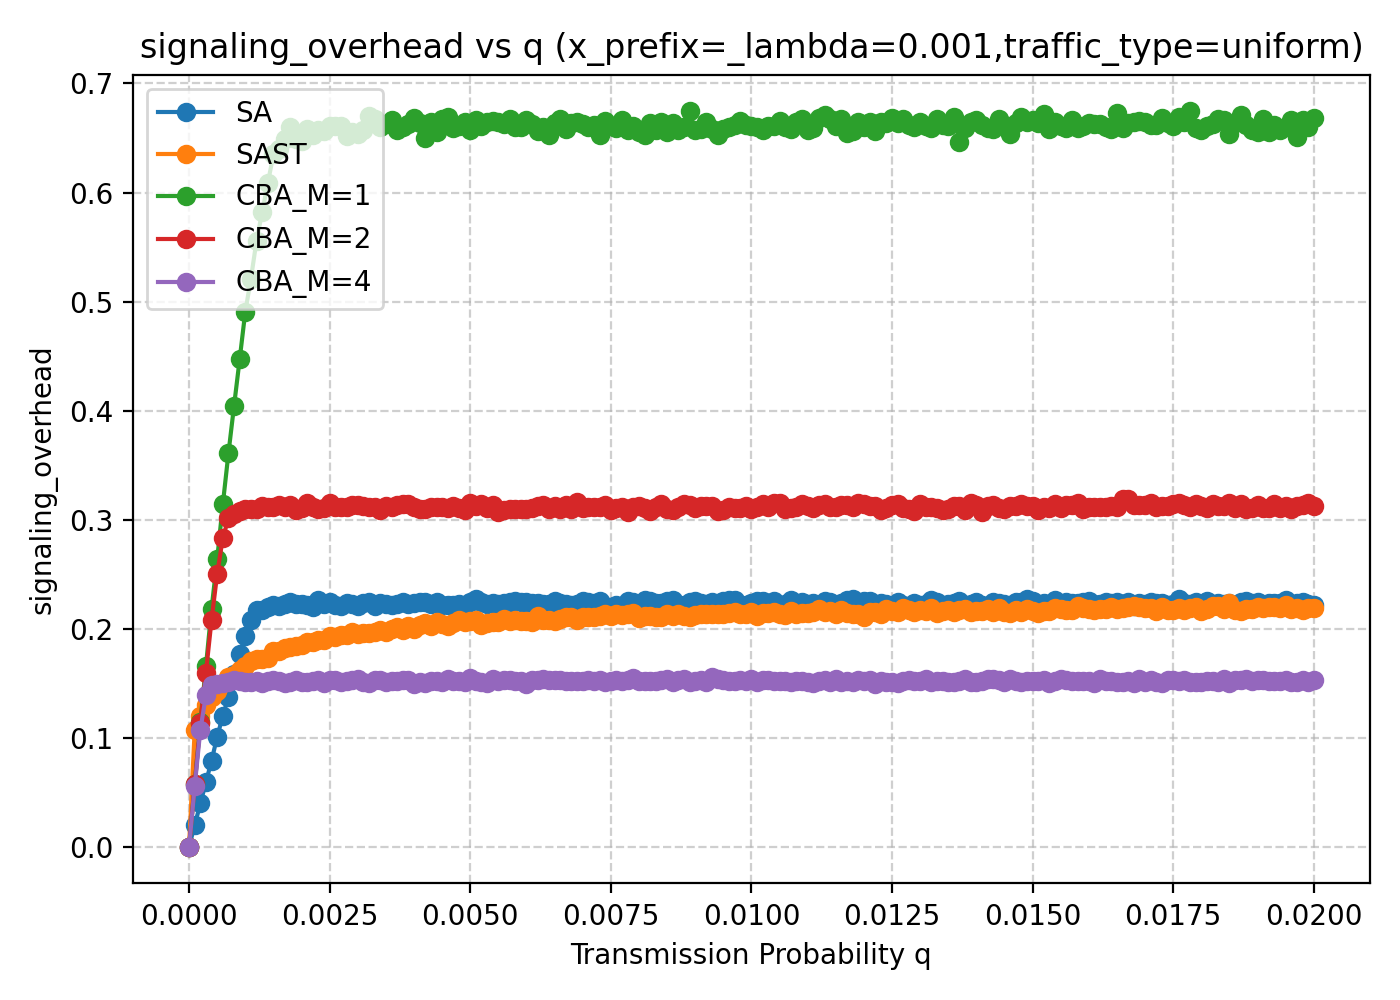
\includegraphics[width=0.24\textwidth]{figure/chap5/signaling_overhead_vs_q_xprefix__lambda=0.001,traffic_type=uniform.pdf}}
%     \subfloat[$\lambda=0.003$]{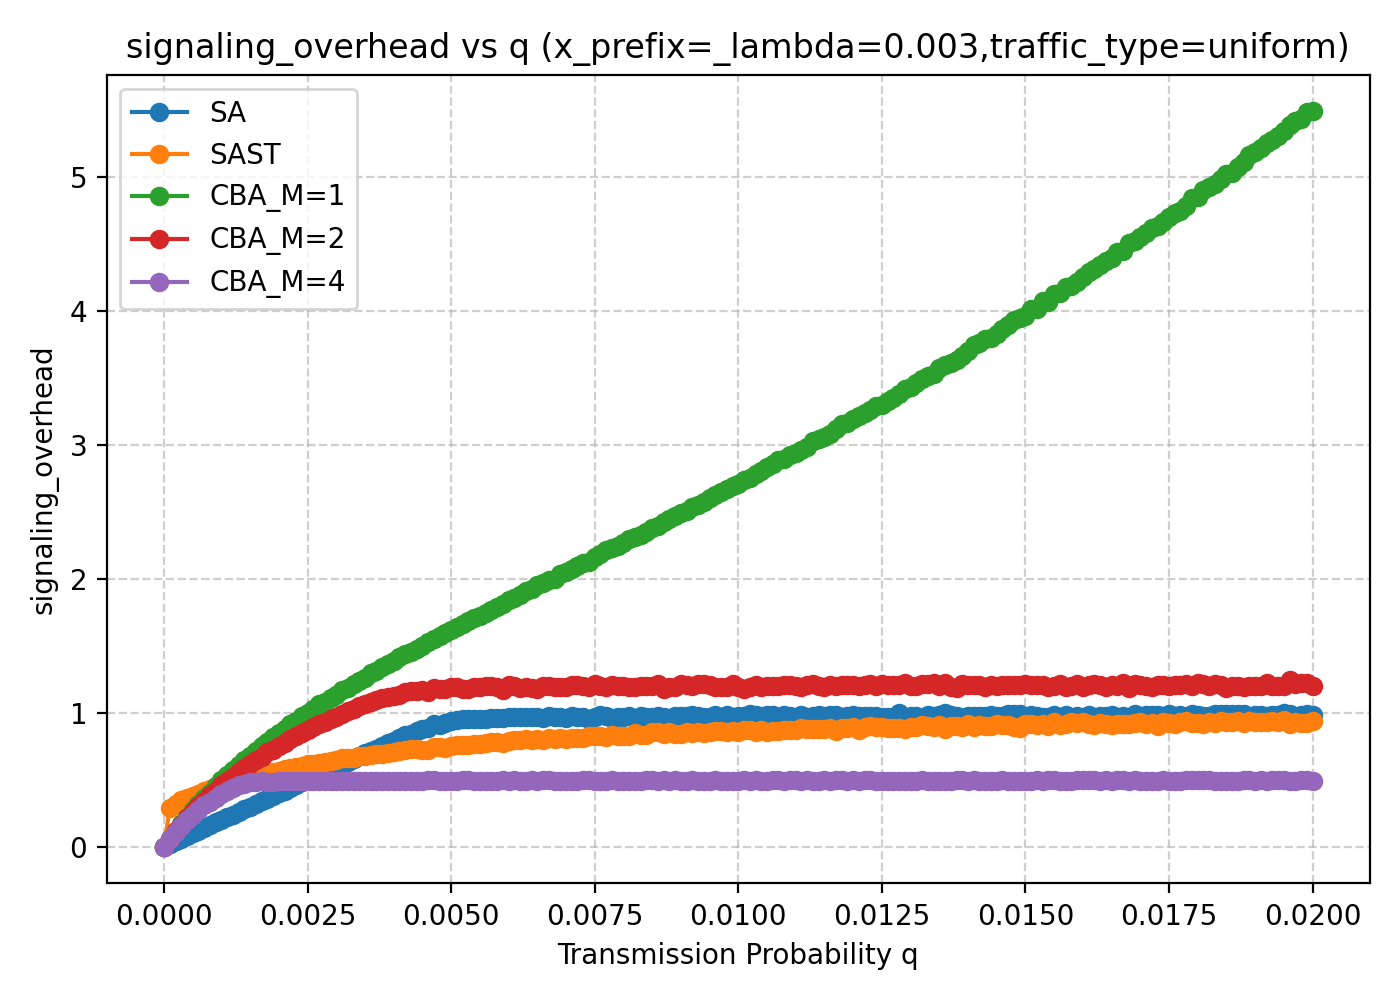
\includegraphics[width=0.24\textwidth]{figure/chap5/signaling_overhead_vs_q_xprefix__lambda=0.003,traffic_type=uniform.pdf}}
%     \subfloat[$\lambda=0.005$]{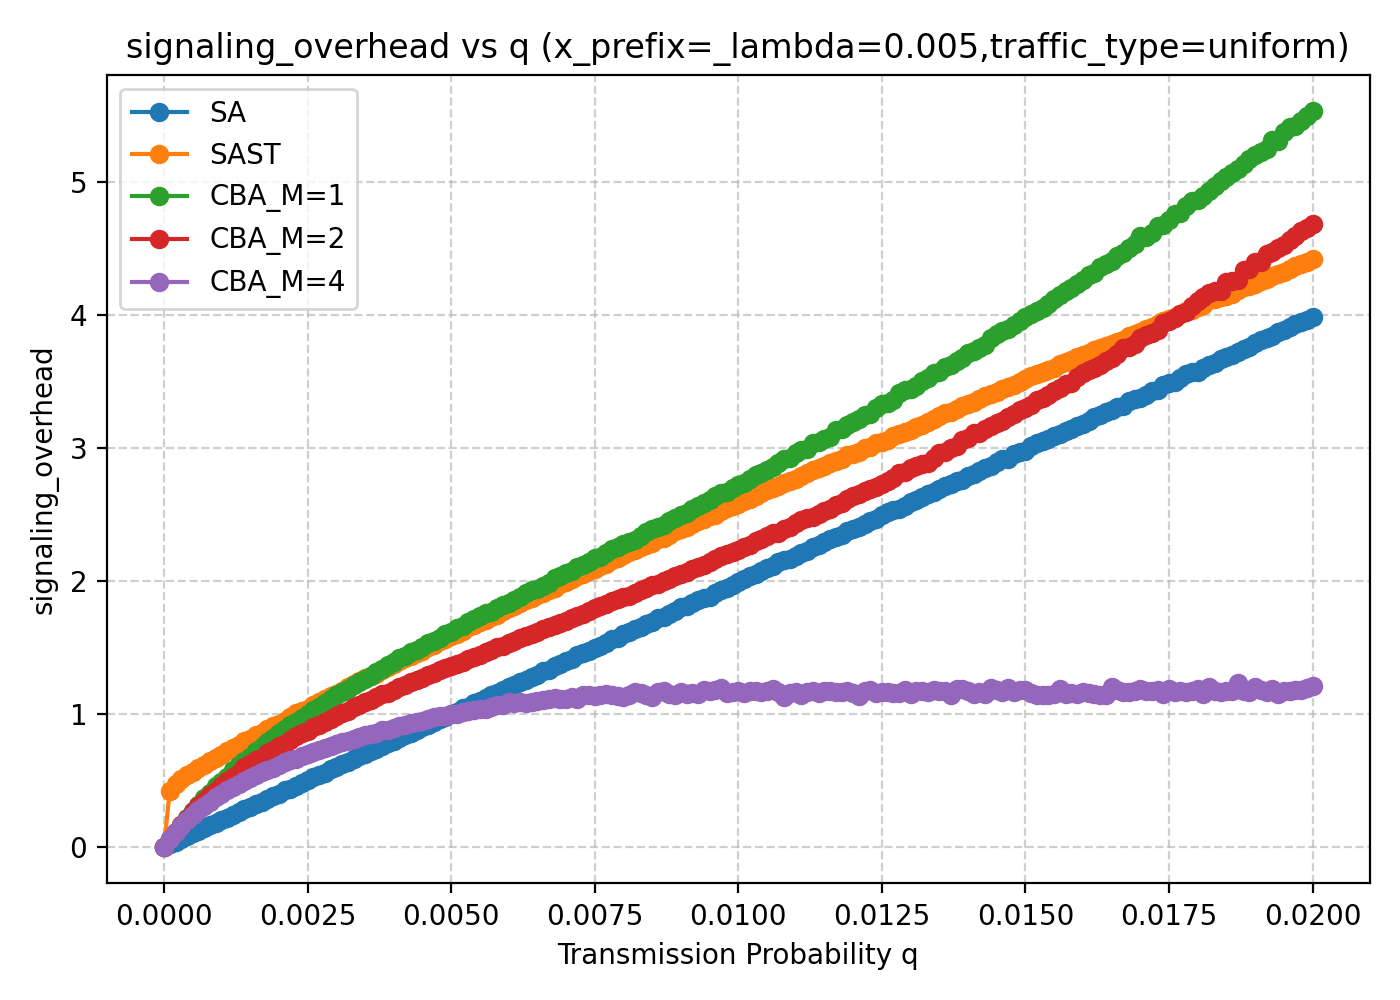
\includegraphics[width=0.24\textwidth]{figure/chap5/signaling_overhead_vs_q_xprefix__lambda=0.005,traffic_type=uniform.pdf}}
%     \caption{不同$\lambda$下均匀流量场景的信令开销$S$随$q$变化对比}
%     \label{fig:signaling_vs_q_uniform}
% \end{figure}


% 上述结果直观展现了在不同流量强度下，三类协议在主要性能指标上的变化趋势，为后续协议选择与参数优化提供了数据支撑。

% === 2. 小结部分只保留简要总结，不再重复上述仿真结果 ===

% =========================================================
% 第 5.3 节：基于多任务深度学习的性能预测模型
% =========================================================

\section{基于多任务深度学习的性能预测模型}
\label{sec:mt_dnn_model}

离散事件仿真器能够在给定协议配置和网络条件下精确评估系统性能，但其计算开销较高。以典型仿真配置（如 $n=100$ 个节点、$T=3\times10^5$ 个时隙）为例，单次样本点的仿真通常需要数十秒甚至数分钟。当需要在多协议、多参数组合及不同流量场景下进行大规模性能评估时，总体仿真时间将迅速累积。本节基于第\ref{subsec:dataset_construction}节构建的仿真数据集，设计并训练一种高效的多任务性能预测模型（Multi-Task Deep Neural Network, MT-DNN）。后文统一简称为性能预测模型。该模型通过共享特征表示并联合学习多个性能指标，实现对系统吞吐量、时延与公平性等关键指标的快速预测。相比传统仿真方法，该模型能够将性能评估时间从分钟级显著降低至毫秒级，从而为后续的协议选择与参数优化提供高效支撑。

\subsection{基于硬参数共享的多任务网络架构}
\label{subsec:hard_sharing}

考虑到网络性能指标之间存在显著的物理耦合性，例如高负载状态通常同时对应吞吐量饱和与时延激增，独立的单任务模型往往忽略了这些内在关联，且训练效率低下。为此，本文设计了基于硬参数共享机制的神经网络架构，该架构在保持参数量可控的同时，能够有效学习多任务间的关联。

\paragraph{架构设计原理}
硬参数共享架构由以下三个核心模块组成：
\begin{itemize}[leftmargin=*]
	\item \textbf{输入归一化层}：采用 LayerNorm 对输入特征进行归一化，消除不同特征量纲差异，稳定梯度流。
	\item \textbf{共享特征提取层}：由两至三层全连接网络堆叠而成，每层均配备 LayerNorm、GELU 激活函数和 Dropout。该部分负责提取所有任务通用的网络状态表征。
	\item \textbf{任务特定头部}：针对每个任务设置独立的单层线性映射，实现从共享特征到任务输出的最终转换。
\end{itemize}

网络的数学描述如下。设输入特征维度为 $D_{\text{in}}$，共享层隐藏维度为 $D_{\text{hidden}}$，共享层深度为 $L$。首先对输入特征与掩码向量逐元素相乘并归一化：
\begin{equation}
	\mathbf{h}^{(0)} = \text{LayerNorm}(\mathbf{X}_{\text{in}} \odot \mathbf{m})
\end{equation}
其中 $\mathbf{m}$ 为掩码向量，用于屏蔽无效参数分量。随后依次进行特征变换和非线性映射：
\begin{equation}
	\mathbf{h}^{(\ell)} = \text{Dropout}\left( \sigma\left( \text{LayerNorm}(\mathbf{W}^{(\ell)} \mathbf{h}^{(\ell-1)} + \mathbf{b}^{(\ell)}) \right) \right), \quad \ell = 1, \ldots, L
\end{equation}
其中 $\sigma$ 表示 GELU 激活函数，Dropout 比率为 0.1。对于第 $k$ 个任务，输出通过线性映射获得：
\begin{equation}
	\hat{y}_k = \mathbf{w}_k \cdot \mathbf{h}^{(L)} + b_k
\end{equation}
各任务输出为连续值，无需额外激活函数。

\begin{table}[htbp]
	\centering
	\caption{多任务性能预测模型的神经网络架构}
	\label{tab:nn_architecture}
	\renewcommand{\arraystretch}{1.25}
	\begin{tabular}{lll}
		\toprule
		\textbf{模块} & \textbf{结构配置} & \textbf{参数说明} \\
		\midrule
		\multirow{2}{*}{输入层} 
		& LayerNorm 
		& 特征归一化以稳定训练过程 \\
		& 掩码乘法 
		& $\mathbf{X}_{\mathrm{in}} \odot \mathbf{m}$，屏蔽无效或缺失特征 \\
		\midrule
		\multirow{5}{*}{共享隐藏层} 
		& FC + LayerNorm 
		& 维度映射 $D_{\mathrm{in}} \rightarrow D_{\mathrm{hidden}}$（如 128） \\
		& GELU + Dropout 
		& 非线性激活与正则化，Dropout 概率 $p=0.1$ \\
		& FC + LayerNorm 
		& 隐藏层维度保持 $D_{\mathrm{hidden}} \rightarrow D_{\mathrm{hidden}}$ \\
		& GELU + Dropout 
		& 激活与正则化 \\
		& 可选第 3 层
		& 深层模式下启用，用于提升模型表达能力 \\
		\midrule
		\multirow{2}{*}{任务输出头} 
		& 每任务独立全连接层 
		& 输出维度为 1 \\
		& 无激活函数 
		& 回归任务，直接输出连续值 \\
		\bottomrule
	\end{tabular}
\end{table}

\begin{figure}[t]
	\centering
	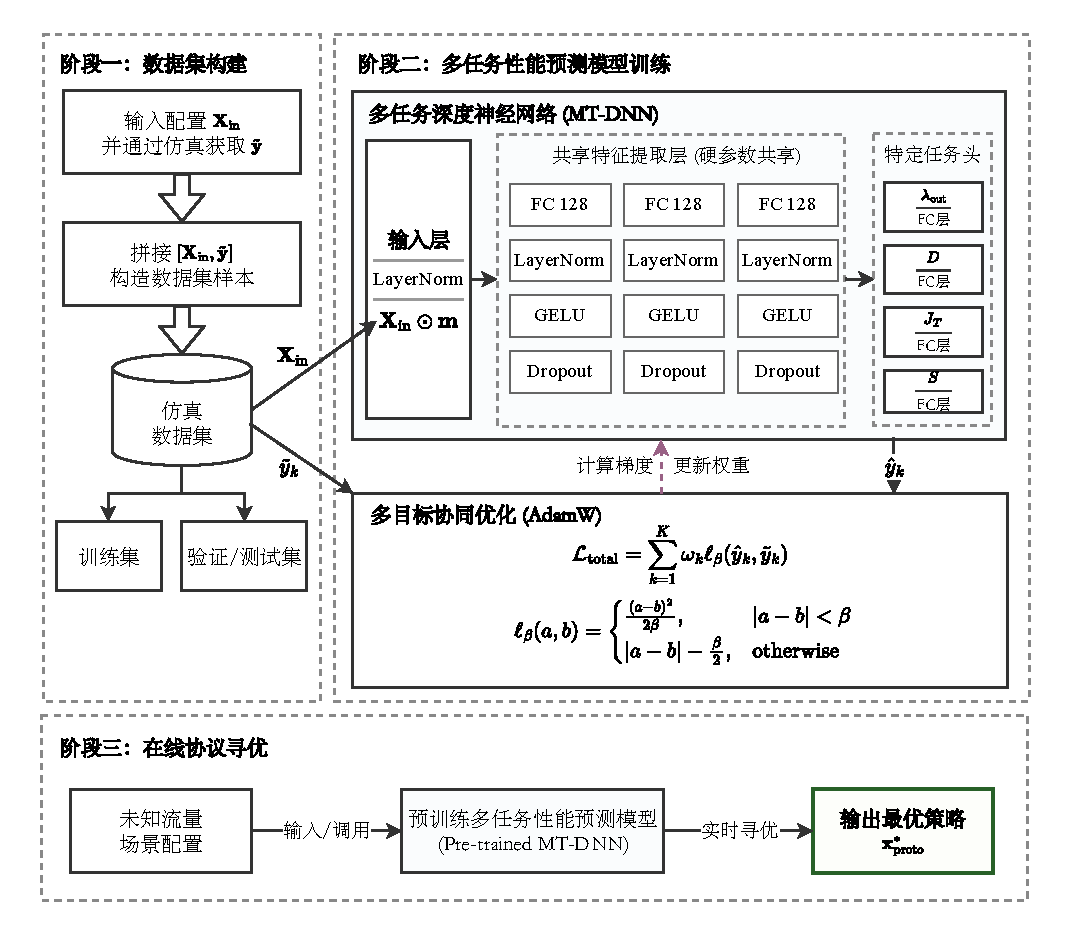
\includegraphics[width=0.95\textwidth]{figure/chap5/神经网络训练流程.pdf}
	\caption{多任务性能预测模型的训练流程示意图}
	\label{fig:nn_training_flow}
\end{figure}

图~\ref{fig:nn_training_flow} 给出多任务性能预测模型的训练流程，包括数据预处理、特征归一化、前向传播、多任务损失计算、参数优化与验证集监控等环节。在标准配置下，模型输入特征维度约为 14，隐藏层宽度为 256，输出端包含 4 个任务分支，参数量约为 71,712--138,016（对应浅层/深层两种结构）。结合前述数据集规模，训练样本量与参数量之比约为 0.086--0.165，可用于评估模型复杂度与样本规模的匹配程度。

\subsection{多目标协同优化与训练策略}
\label{subsec:training}


在多任务学习框架中，不同预测目标通常具有不同的数值尺度与优化难度。若将各任务损失直接等权叠加，梯度更新容易被尺度较大的任务主导，进而削弱对其他关键指标的学习效果。为实现吞吐量、时延、公平性与信令开销四类指标的协同预测，本文采用统一训练策略，将多任务损失建模、正则化约束与自适应优化结合，以提升训练稳定性与泛化能力。

在训练目标设计方面，本文对输入特征采用标准化处理，对输出标签采用最小-最大归一化处理，并将时延指标先进行对数变换以缓解长尾分布影响。在此基础上，采用加权 Smooth L1 作为总体优化目标：
\begin{equation}
\mathcal{L}_{\text{total}}
=
\sum_{k=1}^{K}
\omega_k\,
\ell_{\beta}\!\left(\hat{y}_k,\tilde{y}_k\right),
\end{equation}
其中
\begin{equation}
\ell_{\beta}(a,b)=
\begin{cases}
\dfrac{(a-b)^2}{2\beta}, & |a-b|<\beta,\\[4pt]
|a-b|-\dfrac{\beta}{2}, & \text{otherwise}.
\end{cases}
\end{equation}
式中，$\tilde{y}_k$ 为归一化后的真实标签，$\hat{y}_k$ 为模型预测值，$\omega_k$ 为任务权重系数。本文标准配置下任务权重设置为 $(1,\,3,\,1,\,0.5)$，用于强调时延预测精度并对信令开销施加适度约束，从而实现性能指标与资源开销之间的平衡。

在模型泛化能力提升方面，本文在网络结构中引入 Dropout 与权重衰减，并在反向传播阶段采用梯度裁剪抑制梯度异常，提升深层网络训练的数值稳定性。输入扰动增强机制在框架中已实现，可用于模拟测量噪声与环境不确定性；在本文标准配置中该项默认关闭，以保证基线实验的可重复性与对比公平性。

在模型优化过程中，采用 AdamW 优化器进行端到端参数更新，并结合 ReduceLROnPlateau 学习率调度策略。当验证集指标在设定耐心周期内未见改善时，学习率按比例自动衰减以促进收敛；同时通过早停机制终止无效训练并保留最优参数。模型选择以验证集最大 MAE 为准，并设置目标阈值以实现精度驱动的提前停止，从而在训练效率与泛化性能之间取得平衡。


\subsection{性能预测模型的可视化结果}


\begin{table}[t]
\centering
\caption{性能预测模型实验配置与预测性能结果}
\label{tab:surrogate_model_config_result}
\small
\renewcommand{\arraystretch}{1.25} % 稍微增加行高，提升阅读体验
% 使用 tabular* 并结合 \extracolsep{\fill} 让表格自动撑满左右文本宽度
\begin{tabular*}{\linewidth}{@{\extracolsep{\fill}} l c l c @{}}
\toprule
\multicolumn{4}{c}{\textbf{（一）性能预测模型训练配置}} \\
\midrule
\textbf{参数} & \textbf{设定值} & \textbf{参数} & \textbf{设定值} \\
\midrule
优化器 & AdamW & 基础损失函数 & Weighted Smooth L1 \\
批大小 & 32 & 最大训练轮数 & 800 \\
初始学习率 & $3\times10^{-3}$ & 最小学习率 & $1\times10^{-6}$ \\
学习率衰减系数 & 0.5 & 学习率调度耐心值 & 20 epochs \\
权重衰减系数 & $1\times10^{-6}$ & Dropout率 & 0.1 \\
梯度裁剪阈值 & 1.0 & 早停耐心值 & 80 epochs \\
任务权重 $(\omega_1,\omega_2,\omega_3,\omega_4)$ & $(1,\,3,\,1,\,0.5)$ & Smooth L1参数 $\beta$ & 0.01 \\
模型选择指标 & 验证集最大 MAE & 提前停止目标 & $\max(\mathrm{MAE}) \le 0.005$ \\

\midrule
\multicolumn{4}{c}{\textbf{（二）性能预测模型测试集预测性能}} \\
\midrule
\textbf{性能指标} & \textbf{MSE} & \multicolumn{1}{c}{\textbf{MAE}} & \textbf{$R^2$} \\
\midrule
吞吐量 $\lambda_{\mathrm{out}}$ & 0.000022 & \multicolumn{1}{c}{0.0021} & 0.9997 \\
平均时延 $D$ & 0.001877 & \multicolumn{1}{c}{0.0031} & 0.9599 \\
公平性 $J_T$ & 0.001138 & \multicolumn{1}{c}{0.0037} & 0.6832 \\
信令开销 $S$ & 0.000012 & \multicolumn{1}{c}{0.0022} & 0.9998 \\
\bottomrule
\end{tabular*}
\end{table}


为验证所提出多任务性能预测模型在典型业务场景下的预测能力，本文在统一仿真数据集上对模型进行了训练与测试，并在测试集上评估其对各类系统性能指标的预测精度。实验采用标准监督学习训练流程，相关训练配置与测试结果如表~\ref{tab:surrogate_model_config_result} 所示。

从表~\ref{tab:surrogate_model_config_result} 可以看出，在统一训练配置下，所提出的多任务性能预测模型在测试集上取得了较高的预测精度。其中，吞吐量与信令开销等指标的决定系数均接近 $1$，表明模型能够准确刻画协议配置与系统性能之间的映射关系；对于平均时延与公平性等复杂性能指标，模型同样保持较低的预测误差与较高的拟合优度。总体而言，该性能预测模型能够在保证计算效率的同时实现对关键网络性能指标的高精度预测，从而为后续基于性能预测模型的协议参数优化与自适应接入策略设计提供可靠的性能评估基础。



\begin{figure}[t]
    \centering
    % 第一行：全局共享图例（缩放因子根据实际大小微调，这里设为 0.95 避免溢出）
    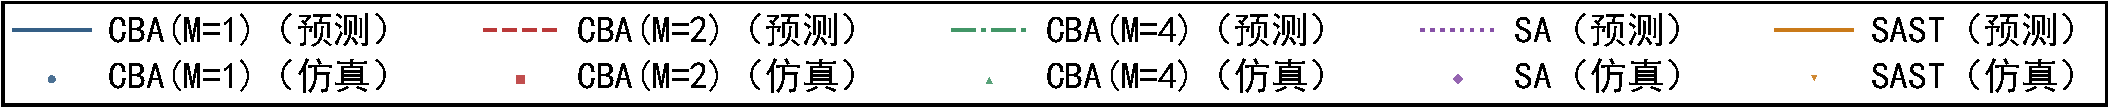
\includegraphics[width=0.99\textwidth, trim=0 0 0 0, clip]{figure/chap5/shared_legend.pdf} \\
    
    % 第二行：子图并排
    \subfloat{
        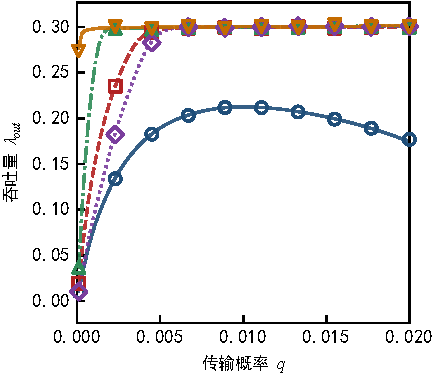
\includegraphics[width=0.49\textwidth]{figure/chap5/5_3_metric_throughput.pdf}
        \label{fig:ai_vs_sim_uniform_003_thr}
    }
    \subfloat{
        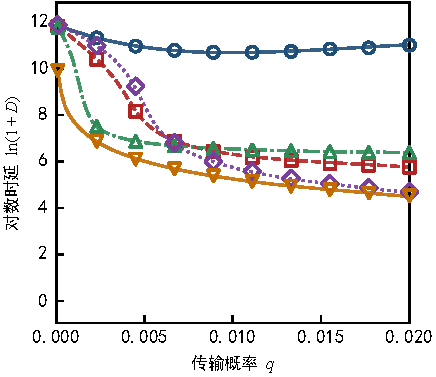
\includegraphics[width=0.49\textwidth]{figure/chap5/5_3_metric_delay.pdf}
        \label{fig:ai_vs_sim_uniform_003_delay}
    } \\
    
    % 第三行：子图并排
    % \subfloat[公平性 $J$]{
    %     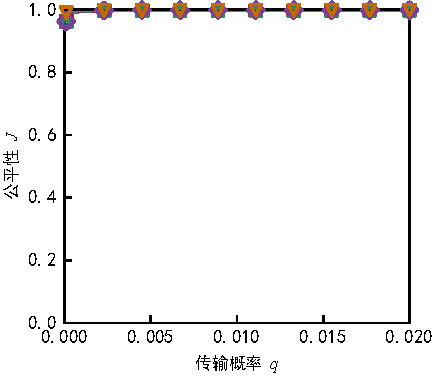
\includegraphics[width=0.49\textwidth]{figure/chap5/5_3_metric_fairness.pdf}
    %     \label{fig:ai_vs_sim_uniform_003_fairness}
    % }
    \subfloat{
        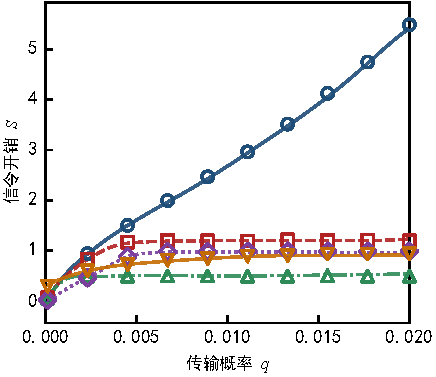
\includegraphics[width=0.49\textwidth]{figure/chap5/5_3_metric_signaling.pdf}
        \label{fig:ai_vs_sim_uniform_003_signaling}
    }
    
    \caption{均匀流量、$\lambda=0.003$ 场景下的模型预测（理论值）与仿真结果（离散点）对比。}
    \label{fig:ai_vs_sim_uniform_003}
\end{figure}

\begin{figure}[t]
    \centering
    % 第一行：全局共享图例（缩放因子根据实际大小微调，这里设为 0.95 避免溢出）
    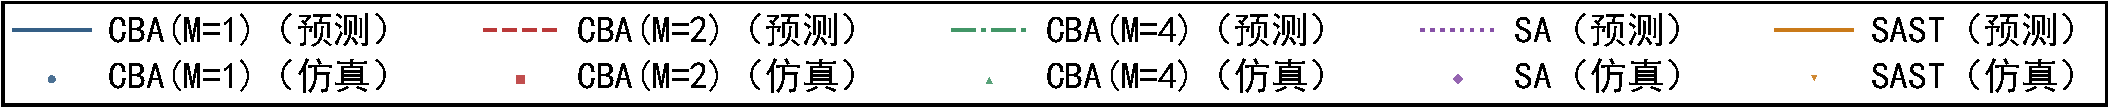
\includegraphics[width=0.99\textwidth, trim=0 0 0 0, clip]{figure/chap5/shared_legend.pdf} \\
	
	\subfloat[吞吐优先]{
		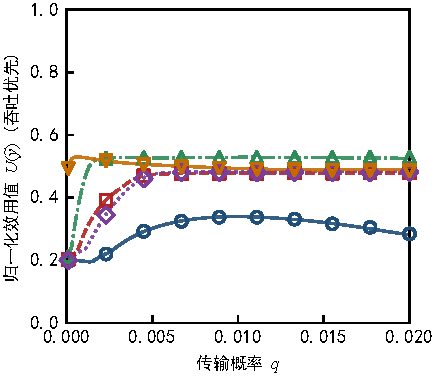
\includegraphics[width=0.48\textwidth]{figure/chap5/5_3_utility_throughput_prio.pdf}
		\label{fig:utility_priority_uniform_003_thr}
	}
	\hfill
	\subfloat[时延优先]{
		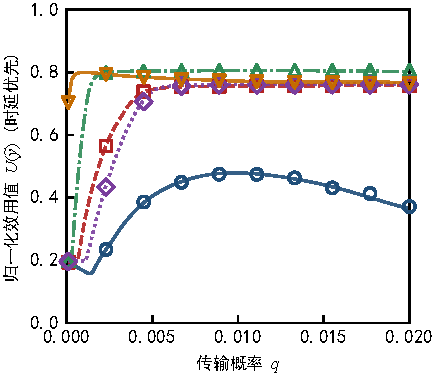
\includegraphics[width=0.48\textwidth]{figure/chap5/5_3_utility_delay_prio.pdf}
		\label{fig:utility_priority_uniform_003_delay}
	}
	\hfill
	\subfloat[信令优先]{
		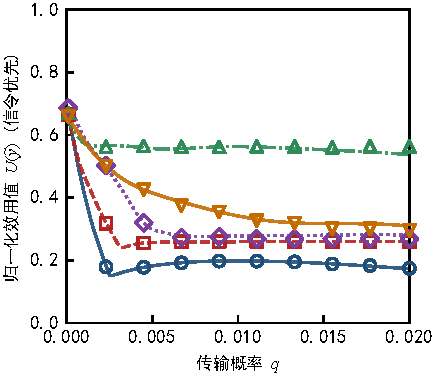
\includegraphics[width=0.55\textwidth]{figure/chap5/5_3_utility_signaling_prio.pdf}
		\label{fig:utility_priority_uniform_003_signaling}
	}
	\caption{均匀流量、$\lambda=0.003$ 场景下，不同权重偏好的综合效用 $U$ 对比。}
	\label{fig:utility_priority_uniform_003}
\end{figure}
\subsection{性能预测模型曲线一致性与效用曲线对比说明}
本小节以均匀流量、单节点到达率 $\lambda=0.003$ 为例，对不同协议参数 $q$ 下的性能曲线进行可视化对比。图~\ref{fig:ai_vs_sim_uniform_003} 中实线为预测、离散点为仿真结果，吞吐量、时延与信令开销三类指标在参数区间内的变化趋势一致，峰值与拐点位置可对齐。公平性指标 $J_T$ 在各配置下基本接近 1、区分度较低，故不再单独绘制其曲线图。

进一步，为反映不同业务偏好下的综合性能，本节同时考察效用函数 $U(\tilde{\mathbf{y}})$ 的变化趋势，并将三种典型权重配置合并展示：吞吐优先、时延优先与信令优先。对应曲线见图~\ref{fig:utility_priority_uniform_003} 的三个子图。三条曲线在峰值位置与拐点处的差异，体现了权重设置对最优参数选择的影响：吞吐优先更倾向于高负载区间的参数组合；时延优先与信令优先则更偏向保守配置以降低排队与控制开销。该对比说明在统一性能预测模型输出基础上，仅需调整权重即可实现面向不同业务目标的快速策略切换。



\section{基于性能预测模型的快速搜索与预测}
在性能预测模型 $f_{\phi}$ 训练完成后，协议优化问题可转化为单次决策窗口内的参数搜索问题。给定业务场景的流量特征 $\mathbf{x}_{\text{traffic}}$，目标是求得统一参数向量 $\mathbf{x}_{\text{proto}}^*$, 即：
\begin{equation}
	\mathbf{x}_{\text{proto}}^* = \arg\max_{\mathbf{x}_{\text{proto}}} U\big(f_{\phi}(\mathbf{x}_{\text{traffic}}, \mathbf{x}_{\text{proto}}, \dots)\big)
\end{equation}
由于 $f_{\phi}$ 的评估开销较低，本文采用直接网格搜索以保证可复现性。针对混合离散—连续参数空间，该方法在候选协议与参数域内逐点评估并选择效用最大值。

在实际业务场景中，网络流量类型与强度具备显著的动态时变性，且协议切换决策与流量突变往往非同步。为贴合工程流程，本文采用滑动观测窗口在线更新流量特征，并在每个决策时刻执行一次快速搜索。具体流程为：
\begin{enumerate}[leftmargin=*]
	\item \textbf{状态观测}：在窗口 $[t-\Delta t, t]$ 内统计流量特征 $\mathbf{x}_{\text{traffic}}$；
	\item \textbf{直接搜索}：对 $\mathcal{P}$ 中各协议进行枚举，并在其参数域内快速搜索；
	\item \textbf{协议自切换}：选择效用最高且满足约束的协议与参数，触发协议切换并下发配置；
\end{enumerate}

为保证对比结果的可复现性与逻辑一致性，本文构建两类验证场景。每类场景均包含连续 10 个观测窗口，单窗口长度为 $3\times10^5$ 个时隙；协议切换与窗口边界同步，决策周期同样设为 $3\times10^5$ 个时隙。每个窗口内均采用直接搜索获得性能预测模型推荐策略，并以离线穷举得到的近似最优效用作为参考上界。

\textbf{场景一：均匀流量、强度递变。} 该场景中流量类型固定为均匀到达（U），仅按预设序列调整归一化平均到达率 $\hat{\lambda}$。具体窗口配置见表~\ref{tab:chap5_scene1_windows}。该序列覆盖低、中、高多档负载，并包含升载与降载过程，用于评估流量形态固定条件下各协议对强度动态的适配能力。

\begin{table}[htbp]
\centering
\caption{场景一的窗口配置（均匀流量、强度递变）}
\label{tab:chap5_scene1_windows}
\renewcommand{\arraystretch}{1.15}
\small
\setlength{\tabcolsep}{5pt}
\begin{tabular}{c c c c}
\toprule
\textbf{窗口} & \textbf{时间区间 $t$} & \textbf{流量类型} & \textbf{$\hat{\lambda}$} \\
\midrule
1  & $[0,3\times10^5)$    & U & 0.10 \\
2  & $[3\times10^5,6\times10^5)$  & U & 0.20 \\
3  & $[6\times10^5,9\times10^5)$  & U & 0.30 \\
4  & $[9\times10^5,12\times10^5)$ & U & 0.70 \\
5  & $[12\times10^5,15\times10^5)$ & U & 0.45 \\
6  & $[15\times10^5,18\times10^5)$ & U & 0.50 \\
7  & $[18\times10^5,21\times10^5)$ & U & 0.55 \\
8  & $[21\times10^5,24\times10^5)$ & U & 0.80 \\
9  & $[24\times10^5,27\times10^5)$ & U & 0.25 \\
10 & $[27\times10^5,30\times10^5)$ & U & 0.10 \\
\bottomrule
\end{tabular}
\end{table}

\textbf{场景二：流量类型与强度联合变化。} 该场景中流量形态与归一化平均到达率在 10 个窗口内同步变化，覆盖均匀（U）、突发（B）、周期（P）三类到达过程，构成“低负载→中负载→高负载→恢复”的循环序列。具体窗口配置见表~\ref{tab:chap5_scene2_windows}。该序列通过引入形态切换及强度升降过程，用于检验系统在流量类型与强度同时变化条件下的综合适配能力。

\begin{table}[htbp]
\centering
\caption{场景二的窗口配置（流量类型与强度联合变化）}
\label{tab:chap5_scene2_windows}
\renewcommand{\arraystretch}{1.15}
\small
\setlength{\tabcolsep}{5pt}
\begin{tabular}{c c c c}
\toprule
\textbf{窗口} & \textbf{时间区间 $t$} & \textbf{流量类型} & \textbf{$\hat{\lambda}$} \\
\midrule
1  & $[0,3\times10^5)$    & U & 0.10 \\
2  & $[3\times10^5,6\times10^5)$  & B & 0.30 \\
3  & $[6\times10^5,9\times10^5)$  & P & 0.50 \\
4  & $[9\times10^5,12\times10^5)$ & U & 0.70 \\
5  & $[12\times10^5,15\times10^5)$ & B & 0.50 \\
6  & $[15\times10^5,18\times10^5)$ & P & 0.30 \\
7  & $[18\times10^5,21\times10^5)$ & U & 0.20 \\
8  & $[21\times10^5,24\times10^5)$ & B & 0.60 \\
9  & $[24\times10^5,27\times10^5)$ & P & 0.40 \\
10 & $[27\times10^5,30\times10^5)$ & U & 0.15 \\
\bottomrule
\end{tabular}
\end{table}

为明确改进来源，本文设置两类基线策略：
\begin{itemize}[leftmargin=*]
	\item \textbf{基线1：单一协议固定参数。} 采用 SA 协议，传输概率 $q=0.01$ 恒定不变，用作静态配置参考。
	\item \textbf{基线2：协议固定、参数可调。} 固定协议为 CBA，仅在协议内调参。对 $q$ 进行网格穷举（有效区间内均匀取 100 个采样点，并在峰值邻域额外加密 50 点），$M\in\{1,2,4\}$ 逐一遍历，取效用最大者作为该窗口的最优配置。
\end{itemize}

实验流程包括生成流量变化序列、提取窗口特征、在线搜索与协议切换，以及对比最优效用曲线与指标趋势。对上述两种场景分别进行实验，结果分别如图~\ref{fig:utility_vs_traffic_uniform} 与图~\ref{fig:utility_vs_traffic_mixed} 所示。

\begin{figure}[t]
	\centering
	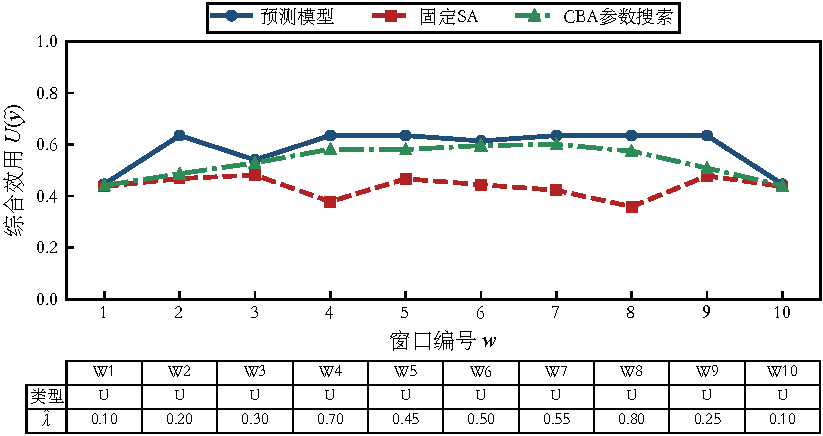
\includegraphics[width=0.99\textwidth]{figure/chap5/utility_dynamic_uniform_0315.pdf}
	\caption{场景一下性能预测模型推荐策略与基线策略的效用对比。横坐标表示按时序排列的协议切换窗口编号，纵坐标表示对应的综合效用 $U(\tilde{\mathbf{y}})$。}
	\label{fig:utility_vs_traffic_uniform}
\end{figure}

\begin{figure}[t]
	\centering
	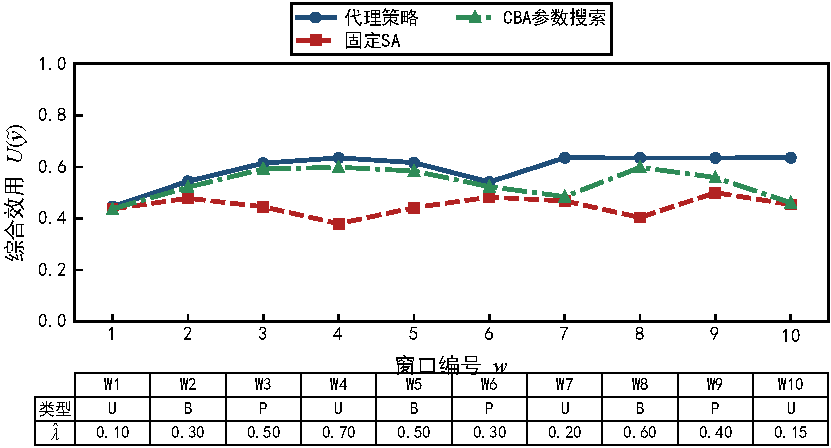
\includegraphics[width=0.99\textwidth]{figure/chap5/utility_dynamic_combined_0315.pdf}
	\caption{场景二下性能预测模型推荐策略与基线策略的效用对比。横坐标表示按时序排列的协议切换窗口编号，纵坐标表示对应的综合效用 $U(\tilde{\mathbf{y}})$。}
	\label{fig:utility_vs_traffic_mixed}
\end{figure}




\section{本章小结}

本章提出了一种基于监督学习的智能协议与参数联合选择方法，旨在解决传统单一接入协议在复杂多变业务场景下的性能局限性。首先，我们设计了一个统一的接入框架，通过标准化的输入特征向量，对不同的业务流量、网络规模和协议参数进行统一建模。随后，为克服传统网络仿真的高时间成本，我们构建了性能预测模型，并利用多任务深度神经网络学习并复现从输入特征到多维性能指标的复杂映射关系。最后，基于训练好的、能够进行毫秒级预测的性能预测模型，将原先难以处理的协议优化问题转化为一个可由高效搜索算法求解的数学问题。

综上所述，本章通过统一框架设计、性能预测模型构建与快速优化求解，为实现随机接入机制的智能化和自适应化提供了完整的理论与实践基础。

        \newclearpage

        \chapter{总结与展望}
\label{chap:conclusion}

\section{工作总结}

随着 B5G/6G 网络向海量连接与多样化业务需求持续演进，传统随机接入机制在复杂物联网场景中的性能瓶颈日益凸显。针对重复竞争开销大、系统效率与公平性难以兼顾、动态场景适配能力不足等问题，全文按照单接入机制理论优化到智能接入协议决策的逻辑主线，展开系统研究。主要工作可归纳如下：
\begin{itemize}

\item 在授权频谱随机接入场景中，针对短报文按包竞争引起的碰撞累积与信令开销问题，提出连续传输增强 Aloha 机制 SAST。理论分析与仿真结果表明，该机制在不改变原有分布式接入结构的前提下，将系统最大数据吞吐量提升至0.5，突破了经典时隙 Aloha 的性能上限$1/e$。
进一步地，所建立的分析结果揭示了连续传输策略通过延长信道占用周期，有效分摊竞争开销的内在机理，使系统吞吐量与接入效率得到同步提升。同时，在5G小数据传输场景中的对比分析表明，相较于两步随机接入方案，该机制在提升吞吐量的同时显著降低信令开销，在饱和条件下可降低约一半，在非饱和条件下降幅可达70\%。
上述结果表明，连续传输机制在维持现有协议架构兼容性的前提下，能够有效提升海量物联网场景下的接入效率与资源利用率，为5G及后续系统中高效随机接入机制的设计提供了理论依据与实现路径。


\item 在非授权频谱场景中，针对 LBT 机制下频繁侦听与退避导致的信道利用率下降问题，本文将连续传输思想引入载波侦听多路访问机制，提出连续传输增强 CSMA 协议 CSMAST。
该机制在保留载波侦听竞争基本流程的基础上，通过在成功接入后支持连续数据传输，有效降低重复竞争带来的开销。考虑空闲侦听、碰撞与成功传输对应时隙长度异构的特性，本文构建了基于吸收马尔可夫链的休假排队模型，对信道假期过程进行刻画，并推导出系统吞吐量闭环数学表达式。在此基础上，引入并且成功推导 Jain 公平性指标 $J_T$的表达式，分析了连续传输机制对系统吞吐量和公平性的影响。理论与仿真结果表明，CSMAST 在同等侦听条件下，可显著提升系统吞吐量大约28.8\%，同时能够在提升信道利用率的同时保持良好的公平性。此外，结果进一步揭示了竞争接入系统中吞吐量与公平性之间的内在权衡关系。

\textcolor{red}{
    \item 在动态业务环境场景中，针对单一接入机制及参数配置在动态业务变化中适配能力不足的问题，构建统一的接入评估与决策框架。该框架通过离散事件仿真对不同接入协议及参数配置在多种业务场景下的性能进行系统采样，形成覆盖多维性能指标的高质量数据集。在此基础上，本文进一步构建多任务学习模型，对吞吐量、时延、公平性及信令开销等关键性能进行联合预测。结果表明，该模型能够准确刻画复杂接入环境中的性能映射关系，实现对多协议性能的高精度快速估计。进一步地，基于所构建的预测模型与效用函数 $U(\tilde{\mathbf{y}})$，设计面向动态业务环境的自适应决策机制，实现协议选择与参数配置的联合优化。实验结果表明，所提出方法能够在保证良好实时性的情况下，获得业务动态变化下获得稳定的性能增益。}
\end{itemize}


\section{研究展望}
在上述研究中，本文围绕随机接入机制的性能优化与动态环境自适应决策问题，分别从单机制增强与多机制协同决策两个层面开展了系统研究，在提升接入效率、降低竞争开销以及实现多性能指标协同优化方面取得了一定进展。然而，随着 B5G/6G 网络向更高密度连接、更复杂业务形态及更动态网络环境持续演进，接入系统在物理信道特性、业务异构性以及系统规模等方面仍面临更加复杂的挑战，现有研究在建模精细性、决策机制鲁棒性及工程实现等方面仍存在进一步拓展空间。基于此，未来可从以下几个方向展开深入研究：
\begin{itemize}
\item 在物理层建模方面，现有分析基于理想碰撞信道模型，假设冲突数据包完全不可恢复，难以刻画实际无线信道中存在的捕获效应与干扰结构。未来可引入多包接收（Multi-Packet Reception, MPR）与干扰消除（Interference Cancellation, IC）等机制，对部分可解码冲突场景进行建模，从而建立跨层耦合接入模型。在此基础上，有望重新刻画本文所提的增强机制的性能上界与稳定性区域，进一步挖掘连续传输机制在复杂信道环境下的性能潜力。

\item 在网络模型方面，现有研究主要基于同质节点假设，未充分考虑多业务类型在时延、可靠性及吞吐需求上的差异。在实际物联网系统中，往往存在不同优先级的异构设备共存的情况。未来可面向异构设备接入场景，构建区分业务类型的随机接入模型，引入优先级机制与差异化接入策略，研究不同业务在共享信道中的资源竞争与性能保障问题，并探索面向服务质量（QoS）约束的异构节点接入机制设计方法。

\item 在智能决策方面，现有方法基于监督学习对接入系统的性能映射关系进行建模，并在此基础上实现协议与参数的自适应决策。然而，该方法依赖于离线仿真数据进行训练，在面对分布发生变化的超复杂动态环境时，其泛化能力与适应能力仍有待提升。未来可进一步研究面向动态环境的在线学习与增量学习方法，使模型能够在运行过程中持续更新，从而提升对未知业务场景的适应能力。此外，现有模型依赖集中式训练与全局数据，在大规模网络中可能带来较高的数据获取与计算开销。未来可探索轻量化模型设计与分布式学习机制，在保证预测精度的同时降低计算复杂度，并使节点能够基于局部信息进行近似决策，从而提升系统的可扩展性与实际部署可行性。

\item 在工程实现方面，现有研究主要基于理论分析与离散事件仿真验证，尚未考虑实际商用系统中的实现约束与真实协议开销。本文所提出的连续传输增强机制在设计上保持了对现有 3GPP 随机接入协议框架的高度兼容性，仅在接入成功后的传输阶段进行扩展，因此具备较低的协议改动成本与良好的工程落地潜力。未来可在此基础上，结合实际系统约束，进一步研究机制在标准协议栈中的实现方式与信令交互过程，并基于软件无线电（Software Defined Radio, SDR）平台开展原型系统设计与实验验证，评估其在真实无线环境中的性能表现、实现复杂度及系统开销，从而推动相关机制向实际通信系统中的应用转化。
\end{itemize}






        \newclearpage
        % \include{docs/Chapter_07}
        % \newclearpage
       % 结语
        % 附录部分
        \backmatter
        % 参考文献
        \makereferences
        \newclearpage

        % % 附录
        \appendix
        \chapter{类型1休假到达过程的概率生成函数PGF推导}
\label{app:proof_lemma1}

本附录推导类型1休假期内新到达数据包量的概率生成函数PGF。在类型1休假期的第一个时隙，可能出现三种情形。

\begin{itemize}
	\item \textbf{情形1}：以概率$qe^{-\theta}$，标记节点向接收机传输数据包，其他$n-1$个节点均不请求传输。此时休假期只持续一个时隙。一个时隙内到达量服从参数为$\lambda$的伯努利分布，其概率生成函数为$I(z)=1-\lambda+\lambda z$。因此，$A_{V1}$在该情形下的概率生成函数为
	\begin{equation}
		G_{A_{V1}}(z)|\text{C1} = 1 - \lambda + \lambda z
	\end{equation}
	
	\item \textbf{情形2}：以概率$(1-q)\theta e^{-\theta}$，标记节点不传输，其他$n-1$个节点中有且仅有一个成功传输。标记节点继续处于休假期。此后，它将依次经历三个阶段：(1) 一个非竞争的时隙；(2) 另一个节点的忙期；(3) 一个新的类型1休假期。因此，情况2下$A_{V1}$的概率生成函数为：
	\begin{equation}
		G_{A_{V1}}(z)|\text{C2} = (1 - \lambda + \lambda z) \times G_{A_{B}}(z) \times G_{A_{V1}}(z)
	\end{equation}
	
	\item \textbf{情形3}：以概率$1-(1-q)\theta e^{-\theta}-qe^{-\theta}$，第一个时隙中无节点成功。标记节点在下一个时隙继续竞争信道。此后，它将经历两个阶段：(1) 一个空闲时隙；(2) 一个类型1的休假期。因此，$A_{V1}$在该情形下的概率生成函数为
	\begin{equation}
		G_{A_{V1}}(z)|\text{C3} = (1 - \lambda + \lambda z) \times G_{A_{V1}}(z)
	\end{equation}
\end{itemize}

基于全概率定律，综合以上三种情形，我们即可得到目标结果。

        \newclearpage
        \chapter{节点在忙期时队列状态$Q \to P$的马尔可夫链建模与概率生成函数推导}
\label{app:proof_lemma2}
%\addcontentsline{toc}{chapter}{忙期服务过程 ($Q \to P$) 的详细推导}

本附录研究节点忙期内的队列状态演化过程。为此，我们构建一个马尔可夫吸收链模型。模型描述从忙期开始队列长度 $Q$ 到忙期结束队列长度 $P$ 的随机变化。
在此基础上，推导 $G_P(z)$ 与 $G_Q(z)$ 的解析关系。

\section{吸收马尔可夫链模型的构建}

为刻画忙期内队列变化与终止机制，我们定义二维随机过程 $\{(L_t,K_t),t=0,1,\dots\}$。
其中
\begin{itemize}
	\item $L_t \in \{0,1,\dots\}$ 表示节点第 $t$ 次传输尝试开始时的剩余队列长度，但不包含正在发送的数据包。若忙期开始时总队列长度为 $Q$，则有 $L_0=Q-1$。这是因为 HoL~数据包已占用信道。
	\item $K_t \in \{0,1\}$ 表示信道状态。$K_t=1$ 表示忙期保持，即本次传输成功并继续发送，节点保持在忙期。$K_t=0$ 表示节点忙期终止，即发生碰撞或发送结束。
\end{itemize}

如图 \ref{fig:absorbing_markov} 所示，该过程可表示为马尔可夫吸收链。
其状态空间划分如下
\begin{itemize}
	\item \textbf{瞬态} $\mathcal{S}_T=\{(j,1)\mid j\ge 0\}$，表示节点持续成功发送，队列中仍有 $j$ 个待发包。系统处于瞬态时，忙期继续。
	\item \textbf{吸收态} $\mathcal{S}_A=\{(j,0)\mid j\ge 0\}$，表示因碰撞或缓存队列清空而终止忙期。进入该状态后发送过程停止，此时的剩余队列长度即为 $P$。
\end{itemize}

\begin{figure}[htbp]
	\centering
	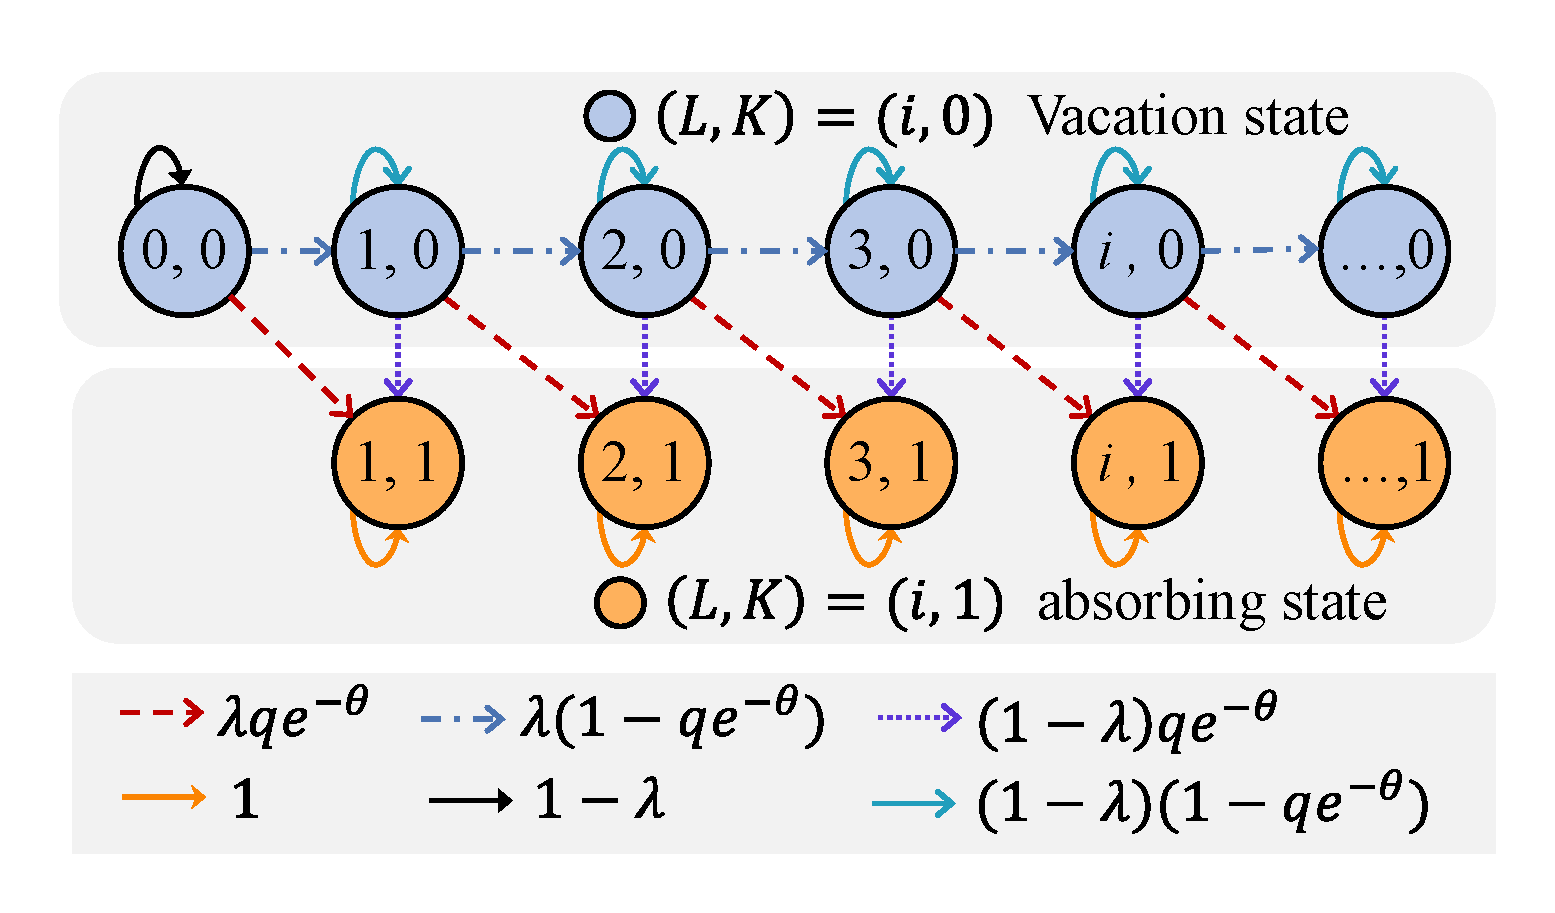
\includegraphics[width=0.8\textwidth]{figure/appdix/P2Q_Absorbing_Markov_chain.pdf}
	\caption{描述忙期内队列演化的吸收马尔可夫链状态转移图}
	\label{fig:absorbing_markov}
\end{figure}

\section{状态转移概率分析}

考虑系统处于瞬态 $(j,1)$。
此时节点正在发送一个数据包，缓存中还有 $j$ 个包。
在一个时隙内，有两类独立过程
\begin{enumerate}
	\item \textbf{新包到达过程}：以概率 $\lambda$到达新包，以概率 $1-\lambda$ 无新包到达。
	\item \textbf{传输过程}：传输成功，即其他 $n-1$ 个节点保持静默的概率为 $e^{-\theta}$；传输失败，即发生碰撞的概率为 $1 - e^{-\theta}$。
\end{enumerate}

综合上述两个过程，下一时刻存在四种转移情形

\begin{enumerate}
	\item \textbf{成功且有新到达}：概率为 $\lambda e^{-\theta}$。发送成功使队列减 1，新包到达使队列加 1。队列长度不变，状态由 $(j,1)$ 转移到 $(j,1)$。
	\item \textbf{成功且无新到达}：概率为 $(1-\lambda)e^{-\theta}$。发送成功且无补充，队列长度减 1。状态由 $(j,1)$ 转移到 $(j-1,1)$。
	\item \textbf{失败且有新到达}：概率为 $\lambda(1-e^{-\theta})$。碰撞使忙期立即结束，新包已进入缓存。状态由 $(j,1)$ 转移到吸收态 $(j+1,0)$。
	\item \textbf{失败且无新到达}：概率为 $(1-\lambda)(1-e^{-\theta})$。碰撞结束忙期且无新包。状态由 $(j,1)$ 转移到吸收态 $(j,0)$。
\end{enumerate}

\section{转移矩阵与基本解}

设忙期开始时队列长度为 $Q$。
当 $Q=1$ 时，系统直接进入吸收态 $(0,0)$，即 $P=0$。
当 $Q\ge 2$ 时，系统从瞬态 $( Q-1,1)$ 出发。
为求吸收概率，我们将状态空间截断为有限维。先设最大队列长度为 $J$，再令 $J\to\infty$。转移矩阵 $\mathbf{M}$ 的标准分块形式为
\begin{equation}
	\mathbf{M} =
	\begin{pmatrix}
		\mathbf{T} & \mathbf{R} \\
		\mathbf{0} & \mathbf{I}
	\end{pmatrix}.
\end{equation}
其中：
\begin{itemize}
	\item $\mathbf{T}$ 是描述瞬态间转移的子矩阵（下双对角矩阵），元素 $t_{j,j} = \lambda e^{-\theta}$，$t_{j, j-1} = (1-\lambda)e^{-\theta}$。
	\item $\mathbf{R}$ 是描述从瞬态进入吸收态的子矩阵，元素 $r_{j, j+1} = \lambda(1-e^{-\theta})$，$r_{j, j} = (1-\lambda)(1-e^{-\theta})$。
\end{itemize}

根据吸收马尔可夫链理论，从任意瞬态 $s_i$ 出发最终被吸收态 $s_j$ 吸收的概率 $b_{ij}$ 构成的吸收概率矩阵为
$$
\mathbf{B}=(\mathbf{I}-\mathbf{T})^{-1}\mathbf{R}.
$$
利用 $\mathbf{T}$ 的下三角结构，可递归求解该矩阵方程。
于是可得从 $( Q-1,1) $ 出发被吸收到 $\langle k,0\rangle$ 的概率，即条件概率 $\Pr\{P=k\mid Q\}$。

经过代数运算，我们得到如下解析解：

\begin{enumerate}
	\item 当 $Q=1$ 时：
	\begin{equation}
		\Pr\{P=0 \mid Q=1\} = 1.
	\end{equation}
	
	\item 当 $Q \ge 2$ 时，对于 $0 \le k \le Q$：
	\begin{equation}
		\Pr\{P=k \mid Q\} = 
		\begin{cases}
			\left[ \frac{(1-\lambda)e^{-\theta}}{1-\lambda e^{-\theta}} \right]^{Q-1}, & k=0 \\
			\frac{(1-\lambda)(1-e^{-\theta})}{1-\lambda e^{-\theta}} \left[ \frac{(1-\lambda)e^{-\theta}}{1-\lambda e^{-\theta}} \right]^{Q-2}, & k=1 \\
			\dots & \vdots \\
			\frac{\lambda(1-e^{-\theta})}{1-\lambda e^{-\theta}}, & k=Q
		\end{cases}
	\end{equation}
\end{enumerate}

\section{PGF关系的建立}

上述条件分布形式较复杂。
在大系统极限下，即 $n\to\infty$ 且 $\lambda\to0$，可利用 PGF 性质得到更简洁表达。
$P$ 表示队列在多次成功发送与新包到达后，被碰撞事件截断时的状态。
据此可证明 $G_P(z)$ 与 $G_Q(z)$ 满足
\begin{equation}
	\label{eq:pgf_P_appendix}
	G_P(z) = G_Q(e^{-\theta}) + \frac{1 - e^{-\theta}}{e^{-\theta} - z} \left[ G_Q(e^{-\theta}) - G_Q(z) \right].
\end{equation}
该式直观地反映了忙期过程对队列分布的过滤作用：$e^{-\theta}$ 项对应于传输成功的概率流，而分母中的 $e^{-\theta}-z$ 项则体现了队列长度随时间步的演化特征。这一结论直接支持了正文中关于 $p_0 = G_P(0)$ 的闭式求解。

        \newclearpage
        \chapter{队列几何分布性质与尝试速率定点方程推导}
\label{app:proof_theorem_fixed_point}

本附录给出定理\texorpdfstring{~\ref{thm:geometric_Q}}{}的详细推导。
目标有两点。
第一，证明在大系统极限下 $Q$ 近似服从几何分布。
第二，推导尝试速率 $\theta$ 的定点方程。

\section{队列分布的几何近似证明}

我们采用猜想与验证方法。
先假设忙期开始时队列长度 $Q$ 服从参数为 $\alpha$ 的几何分布。
当 $Q\ge1$ 时，有 $\Pr\{Q=k\}=\alpha(1-\alpha)^{k-1},\ k\ge1$。
其 PGF 为
\begin{equation}
	\label{eq:GQ_ansatz}
	G_Q(z) = \frac{\alpha z}{1 - (1 - \alpha) z}.
\end{equation}

首先，利用附录 B 的耦合关系
$$
G_P(z)\approx\frac{1-e^{-\theta}}{e^{-\theta}-z}[G_Q(e^{-\theta})-G_Q(z)]
$$
在大 $n$ 极限下可忽略常数项偏差。
将式~(\ref{eq:GQ_ansatz}) 代入并令 $z=0$，得到缓存清空概率 $p_0$
\begin{equation}
	\label{eq:p0_alpha}
	p_0 = G_P(0) = \frac{\alpha}{1 - (1 - \alpha) e^{-\theta}}.
\end{equation}

其次，节点视角下有队列迭代关系 $Q=P+A_V$。
其 PGF 满足
\begin{equation}
	\label{eq:GQ_recursion_app}
	G_Q(z) = p_0 G_{A_{V_0}}(z) + [G_P(z) - p_0] G_{A_{V_1}}(z).
\end{equation}
利用正文中的近似关系
$
G_{A_{V_0}}(z)\approx 1,\quad G_{A_{V_1}}(z)\approx 1-\lambda\overline{V}_1+\lambda\overline{V}_1 z,
$
其中仅保留 $\lambda\to0$ 时的一阶项。
将其代入式~(\ref{eq:GQ_recursion_app}) 并整理。
可得到右侧仍可化为 $G_Q(z)$ 的同型表达。
这验证了几何分布假设的自洽性。

通过系数匹配，可得参数 $\alpha$ 与系统参数的关系
\begin{equation}
	\alpha = 1 - \frac{\theta}{n q}.
\end{equation}
将该式代回式~(\ref{eq:p0_alpha})，即可得到正文式~(\ref{eq:p0_closed_form}) 的 $p_0$ 闭式解
\begin{equation}
	p_0 = \frac{1 - \frac{\theta}{n q}}{1 - \frac{\theta e^{-\theta}}{n q}}.
\end{equation}

\section{定点方程的推导}

由流量守恒，在非饱和稳态下尝试速率 $\theta$ 满足
\begin{equation}
	\theta = n q \left( 1 - \frac{p_0}{\overline{B}} \right).
\end{equation}
利用信道忙期与信道假期的关系 $\overline{B} = \frac{\hat{\lambda}}{1 - \hat{\lambda}} \overline{V}_c$，以及信道假期公式 $\overline{V}_c = \frac{e^{\theta}}{\theta} - p_0$，我们可以将 $\overline{B}$ 表示为：
\begin{equation}
	\overline{B} = \frac{\hat{\lambda}}{1 - \hat{\lambda}} \left( \frac{e^{\theta}}{\theta} - p_0 \right).
\end{equation}

将上述 $\overline{B}$ 和 $p_0$ 的表达式代入 $\theta$ 的定义式中：
\begin{equation}
	\frac{\theta}{n q} = 1 - \frac{p_0 (1 - \hat{\lambda})}{\hat{\lambda} (\frac{e^{\theta}}{\theta} - p_0)}.
\end{equation}
经移项、通分和化简，消去 $p_0$ 的分母项。
最终得到关于 $\theta$ 的隐函数方程
\begin{equation}
	\frac{e^{\theta}}{\theta} + \frac{\theta}{n q} - \frac{1}{n q} = \frac{1}{\hat{\lambda}}.
\end{equation}
这就是定理\texorpdfstring{~\ref{thm:fixed_point_theta}}{}中的定点方程。
该方程表明，尝试速率 $\theta$ 由 $n$、$q$ 与总业务负载 $\hat{\lambda}$ 唯一决定。

        \newclearpage
        \chapter{经典CSMA饱和吞吐量的统一参数推导}
\label{app:classic_csma}

本附录基于休假排队分析框架，重新推导经典CSMA的饱和吞吐量。
推导采用与正文一致的参数体系。
结果可作为与 CSMAST~比较的理论基准。

\section{统一参数表示与模型设定}

在已有文献中，例如 \cite{2013_DaiCSMA}，经典CSMA的最大吞吐量常以传播时延参数 $a$ 表示。
该文献采用状态时长设定
$$
\tau_S=1+a,\quad \tau_F=(x+1)a,\quad \tau_I=a.
$$
由此得到的最大吞吐量表达式包含 Lambert W 函数
\begin{equation}
	\hat{\lambda}_{\text{max}} = \frac{-W_{0}\left(-\frac{1}{x(1+1/x)}\right)}{xa-(1-xa)\,W_{0}\left(-\frac{1}{x(1+1/x)}\right)}.
\end{equation}
为统一比较维度，本文不固定参数 $a$。
我们直接使用状态时长参数 $\tau_S$、$\tau_F$ 与 $\tau_I$ 进行推导。

在本章模型下，经典 CSMA 可视为 CSMAST 的特例。
两者关键差异在于忙期构造方式。
在 CSMAST 中，节点若未发生碰撞即可连续发送，因此忙期内成功发送次数服从参数为 $1-p_0$ 的几何分布，其均值为
$$
\overline{B}_{st}=\frac{\tau_S}{1-e^{-\theta}}.
$$
在经典 CSMA 中，每次竞争后只发送一个数据包。
发送结束后节点立即释放信道并重新竞争。
因此其忙期 $B_{cl}$ 为常数，满足 $\overline{B}_{cl}=\tau_S$。
两种机制在竞争接入阶段采用相同的 LBT~与退避规则。
因此信道假期均值 $\overline{V}_c$ 可沿用前文结论：
\begin{equation}
	\overline{V}_c = \frac{p_{2}\tau_{F}+p_{0}\tau_{I}}{p_{1}},
\end{equation}
其中，$p_0 = e^{-\theta}$、$p_1 = \theta e^{-\theta}$ 和 $p_2 = 1 - p_0 - p_1$ 分别对应无传输、成功接入和发生碰撞的概率（$\theta = nq$）。

\section{吞吐量表达式与最优传输概率}

将 $\overline{B}_{cl}$ 与 $\overline{V}_c$ 代入吞吐量定义式，并引入有效传输修正因子 $\eta=(\tau_S-\tau_I)/\tau_S$，可得经典CSMA在饱和状态下的通用吞吐量表达式
\begin{equation}
	\label{eq:classic_csma_throughput}
	\hat{\lambda}_{\text{out}}^{\text{cl}} = \frac{\tau_{S}-\tau_{I}}{\tau_{S}} \cdot \frac{\overline{B}_{cl}}{\overline{B}_{cl}+\overline{V}_{c}} = \frac{\tau_{S}-\tau_{I}}{\tau_{S}+\frac{p_{2}\tau_{F}+p_{0}\tau_{I}}{p_{1}}}.
\end{equation}

为求理论容量上界，将 $\hat{\lambda}_{\text{out}}^{\text{cl}}$ 视为 $q$ 的函数。
求解最优化条件 $\frac{d\hat{\lambda}_{\text{out}}^{\text{cl}}}{dq}=0$ 后，得到最优传输概率
\begin{equation}
	\label{eq:optimal_q_classic}
	q^{*} = \frac{1 + W_{0}\left(\frac{\tau_{I}-\tau_{F}}{\tau_{F} e}\right)}{n},
\end{equation}
其中 $W_0(\cdot)$ 表示 Lambert W 函数主支\cite{2022_LambertW}。
将 $q^{*}$ 代回式 \eqref{eq:classic_csma_throughput}，即可得到正文图 \ref{fig:comparison_classic} 中经典CSMA曲线的理论上界。

        \newclearpage
        %后记
        \backmatter
        %包括硕士期间发表的与毕业论文相关的已发表论文或被鉴定的技术成果、发明专利等成果，应在成果目录中列出。
\chapter{攻读硕士学位期间相关的科研成果目录}

\setlist[enumerate]{label= \arabic*.}
\begin{enumerate}
	\item 作者攻读硕士期间发表的学术论文
	\setlist[enumerate]{label= [\arabic*]}
	\begin{itemize}
%	  \item  \textbf{XXX}, XXX, XXX, et al. XXX[C]// 2020 IEEE/CIC International Conference on Communications in China (ICCC). IEEE, 2020: 1068-1073.（EI收录，与论文第二、三章内容有关）
    \item \textbf{W. Zhu}, W. Zhan, M. Liu, and J. Qiu. Modeling and Performance Optimization of Slotted Aloha with Successive Transmission. In Proceedings of the International Conference on Wireless Communications and Signal Processing (WCSP), Hefei, China, 2024.（EI收录，与论文第二、三章内容有关）
    \item \textbf{ W. Zhu}, W. Zhan, X. Sun, X. Chen, and Y. Jiang. Boosting Slotted Aloha with Successive Transmission: Modeling and Performance Optimization. //IEEE Transactions on Communications, to appear, 2025. （SCI收录，与论文第二、三章内容有关）
	\end{itemize}


	\item 作者攻读硕士期间申请的发明专利
	\setlist[enumerate]{label= (\arabic*)}
	\begin{itemize}
%	  \item XXX，\textbf{XXX}，XXX，等。XXX：中国，XXX.X[P]。2021.（已受理）（与论文第五章内容有关）
	  \item \textbf{朱威龙}，林衍涵，詹文，孙兴华。一种面向5G 网络的随机接入过程连续传输方法：中国，202510995725.7[P]。2025-09-22.（与论文第五章内容有关）
	\end{itemize}


	\item 论文投稿
	\setlist[enumerate]{label= (\arabic*)}
	\begin{itemize}

%	  \item  XXX, \textbf{XXX}, XXX, et al. XXX. //（ IEEE Transactions on Communications 在审）（与论文第二、三、四章内容有关）
	  \item Sun X, \textbf{W Zhu}, XXX. //（ IEEE Transactions on Communications 在审）（与论文第二、三、四章内容有关）
	\end{itemize}

	\item 作者攻读硕士期间参与的科研项目
	\setlist[enumerate]{label= (\arabic*)}
	\begin{itemize}
	  %\item [(1).]参与广东省自然科学基金面上项目“XXX”，项目编号：XXX，研究年限：2019.10-2022.9.
	  \item [(1).]参与广东省自然科学基金面上项目“XXX”，项目编号：XXX，研究年限：XX.XX-XX.XX.

	  %\item [(2).]参与中国科学院无线传感网与通信重点实验室开放课题“XXX”，项目编号：XXX，研究年限：2019.10-2021.8.
	  \item [(2).]参与中国科学院无线传感网与通信重点实验室开放课题“xxx”，项目编号：xxx，研究年限：XX.XX-XX.XX.

	  %\item [(3).]参与广东省重点领域研发计划项目“XXX”，项目编号：XXX，研究年限：2020.10-2023.12.
	  \item [(3).]参与广东省重点领域研发计划项目xxx”，项目编号：xxx，研究年限：XX.XX-XX.XX.


	\end{itemize}


	
\end{enumerate}     % 科研成果目录
        \newclearpage
% %
%        \chapter{致谢}

先感谢我自己坚持写这个大论文。

\vskip 108pt
\begin{flushright}
	朱威龙\makebox[1cm]{} \\
	\today
\end{flushright}

    % 致谢
%        \newclearpage
% %
    %    \include{docs/Postscript}    % 中山大学学位论文版权使用授权书
    %    \newclearpage

\end{document}

